\chapter*{第五章 空间直线与平面}

\section*{一、平面及其基本性质}

\subsection*{【典型题型和解题技巧】}

1. 公理 1 及其作用.

公理 1 如果一条直线上的两个点在一个平面上, 那么这条直线上所有的点都在这个平面上.

公理 1 的作用有以下两点:

(1)证明点在平面上；

(2)证明直线在平面上.

2. 公理 2 及其推论, 公理 2 及其推论的作用.

公理 2 经过不在一条直线上的三点, 有且只有一个平面.

推论 1 经过一条直线和这条直线外一点, 有且只有一个平面.

推论 2 经过两条相交直线, 有且只有一个平面.

推论 3 经过两条平行直线, 有且只有一个平面.

公理 2 及其推论的作用有:

(1)作辅助平面；

(2)证明平面的唯一性,即证明两个平面重合.

作辅助平面和平面几何中作辅助直线的作用是一样的, 可以为解题开拓思路. 随着立体几何内容的深入, 辅助面将被频繁应用.

3. 公理 3 及其作用.

公理 3 如果两个平面有一个公共点, 那么它们有且只有一条通过这个点的公共直线.

公理 3 的作用有:

(1)确定两个平面的交线；

(2)证明三点共线或证明点在直线上；

(3)确定直线和平面交点的位置.

\textbf{例 1} 在正方体 ${ABCD} - {A}^{\prime }{B}^{\prime }{C}^{\prime }{D}^{\prime }$ 中,画出平面 ${AB}{C}^{\prime }{D}^{\prime }$ 和平面 ${A}^{\prime }{B}^{\prime }{CD}$ 的交线.

\textbf{解} 如图 1,连接 $A{D}^{\prime }$ 和 ${A}^{\prime }D$ 交于点 $M$ . 连接 $B{C}^{\prime }$ 和 ${B}^{\prime }C$ 交于点 $N$ .

\begin{center}
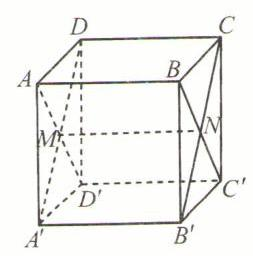
\includegraphics[width=0.2\textwidth]{bodyxb/src/bo_d20aucref24c73anc48g_128_1232_1887_253_256_0.jpg}

(图 1)
\end{center}



$\because M \in$ 直线 $A{D}^{\prime },A{D}^{\prime } \subset$ 平面 ${AB}{C}^{\prime }{D}^{\prime }$，$\therefore M \in$ 平面 ${AB}{C}^{\prime }{D}^{\prime }$ ;

又 $M \in$ 直线 ${A}^{\prime }D,{A}^{\prime }D \subset$ 平面 ${A}^{\prime }{B}^{\prime }{CD}$，$\therefore M \in$ 平面 ${A}^{\prime }{B}^{\prime }{CD}$ .

因此，点 $M$ 是平面 ${AB}{C}^{\prime }{D}^{\prime }$ 和平面 ${A}^{\prime }{B}^{\prime }{CD}$ 的公共点. 同理,点 $N$ 也是平面 ${AB}{C}^{\prime }{D}^{\prime }$ 和平面 ${A}^{\prime }{B}^{\prime }{CD}$ 的公共点. 

连接 ${MN}$ ,根据公理 3,可知直线 ${MN}$ 是平面 ${AB}{C}^{\prime }{D}^{\prime }$ 和平面 ${A}^{\prime }{B}^{\prime }{CD}$ 的交线.

注意(1)不要把两个平面的公共点说成是两个平面的交点;

(2)要确定两个平面的交线,关键在于确定两个平面的两个公共点,这两个公共点的连线就是这两个平面的交线.

\textbf{例 2} 在正方体 ${ABCD} - {A}^{\prime }{B}^{\prime }{C}^{\prime }{D}^{\prime }$ 中,点 $P$ 在棱 $C{C}^{\prime }$ 上,画出直线 ${AP}$ 和平面 ${A}^{\prime }{B}^{\prime }{C}^{\prime }{D}^{\prime }$ 的交点.

\textbf{解} 如图 2,连接 ${AC},{A}^{\prime }{C}^{\prime }$ . 显然, ${A}^{\prime }{C}^{\prime }$ 是平面 $A{A}^{\prime }{C}^{\prime }C$ 和平面 ${A}^{\prime }{B}^{\prime }{C}^{\prime }{D}^{\prime }$ 的交线. 

设点 $Q$ 是直线 ${AP}$ 和平面 ${A}^{\prime }{B}^{\prime }{C}^{\prime }{D}^{\prime }$ 的交点,则 $Q \in$ 平面 ${A}^{\prime }{B}^{\prime }{C}^{\prime }{D}^{\prime }$ ,而 $Q \in  {AP},{AP} \subset$ 平面 $A{A}^{\prime }{C}^{\prime }C$ ,所以 $Q \in$ 平面 $A{A}^{\prime }{C}^{\prime }C$ ,故点 $Q$ 是平面 ${A}^{\prime }{B}^{\prime }{C}^{\prime }{D}^{\prime }$ 和平面 $A{A}^{\prime }{C}^{\prime }C$ 的公共点. 根据公理 3,点 $Q$ 一定在这两个平面的交线 ${A}^{\prime }{C}^{\prime }$ 上.

\begin{center}
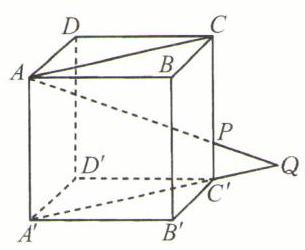
\includegraphics[width=0.2\textwidth]{bodyxb/src/bo_d20aucref24c73anc48g_129_1078_588_305_250_0.jpg}

(图 2)
\end{center}



延长 ${AP}$ 交 ${A}^{\prime }{C}^{\prime }$ 的延长线于点 $Q$ ,点 $Q$ 即直线 ${AP}$ 和平面 ${A}^{\prime }{B}^{\prime }{C}^{\prime }{D}^{\prime }$ 的交点.

注意： 要确定直线 $l$ 和平面 $\alpha$ 的交点,关键在于确定直线 $l$ 所在的平面和平面 $\alpha$ 的交线 $m$ ,而直线 $l$ 与 $m$ 的交点即为所求.

\textbf{例 3} 已知 $E,F,G,H$ 分别是空间四边形 ${ABCD}$ 边 ${AB},{AD},{CB},{CD}$ 上的点,且直线 ${EF}$ 和 ${HG}$ 交于点 $P$ (如图 3),求证:点 $B,D,P$ 在同一条直线上.

\textbf{证明} $\because$ 直线 ${EF} \cap$ 直线 ${HG} = P,\therefore P \in$ 直线 ${EF}$ ,

\begin{center}
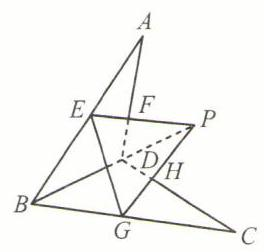
\includegraphics[width=0.2\textwidth]{bodyxb/src/bo_d20aucref24c73anc48g_129_1124_1206_264_252_0.jpg}

(图 3)
\end{center}


而 ${EF} \subset$ 平面 ${ABD},\therefore P \in$ 平面 ${ABD}$ .

同理, $P \in$ 平面 ${CBD}$ ,即点 $P$ 是平面 ${ABD}$ 和平面 ${CBD}$ 的公共点. 显然,点 $B,D$ 也是平面 ${ABD}$ 和平面 ${CBD}$ 的公共点,由公理 3 知,点 $B,D$ , $P$ 都在平面 ${ABD}$ 和平面 ${CBD}$ 的交线上,即点 $B,D,P$ 在一条直线上.

注意(1)要证明三点在同一条直线上,只需证明这三点都是两个平面的公共点;

(2)要证明一点在一条直线上,只需证明这个点是两个平面的公共点,这条直线是两个平面的交线.

\subsection*{【训练题】}

\begin{center}  \textbf{(A)} \end{center}
\begin{enumerate}
    \item 已知点 $P$ 在直线 $l$ 上, $l$ 在平面 $\alpha$ 上,则 $P,l,\alpha$ 之间的关系是\dotfill{(\kh{B})}
    \xx{$P \in  l \in  \alpha$}{$P \in  l \subset  \alpha$}{$P \subset  l \in  \alpha$}{$P \subset  l \subset  \alpha$}
    \begin{jieda}
        点是(三维)空间的元素,直线和平面都是由点构成的集合,因此有 $P \in  l \subset  \alpha$
    \end{jieda}
    \item 用集合符号表示“点 $P$ 在直线 $l$ 外, $l$ 在平面 $\alpha$ 上”,正确的是 \dotfill{(\kh{B})}
    \xx{$P \notin  l,l \in  \alpha$}{$P \notin  l,l \subset  \alpha$}{$P \not\subset l,l \in  \alpha$}{$P \not\subset l,l \subset  \alpha$}
    \begin{jieda}
        点是(三维)空间的元素,直线和平面都是由点构成的集合,因此有 $P \notin  l,l \subset  \alpha$
    \end{jieda}
    \item 下列四个条件中,能确定一个平面的是\dotfill{(\kh{C})}
    \xx{空间任意三点}{空间两条直线}{两条平行直线}{一条直线和一个点}
    \begin{jieda}
        选项 C 即公理 2 的推论 3. 其余 3 个选项的反例如下: 对于选项 A,空间内共线的三点; 对于选项 B,两条异面直线；对于选项 D,该直线恰好经过该点.
    \end{jieda}
    \item 已知空间中四点, 如果其中任意三点都不共线, 那么经过其中三个点的平面共有 \dotfill{(\kh{D})}
    \xx{一个或两个}{一个或三个}{两个或三个}{一个或四个}
    \begin{jieda}
        记4个点为 $A,B,C,P$ ,由题意,记 $A,B,C$ 三点确定平面 $\alpha$ .
        \begin{dingautolist}{172}
            \item $P \in  \alpha$ ,则这 4 点共面,经过任意三个点的平面仅有平面 $\alpha$ 一个.
            \item $P \notin  \alpha$ ,则平面 $\alpha$ 、平面 ${PAB}$ 、平面 ${PBC}$ 、平面 ${PAC}$ 两两不重合(反证法:若任意两个平面重合,则 $A$ , $B,C,P$ 四点共面,从而 $P \in  \alpha$ ,矛盾),此时经过其中三个点的平面共有四个.
        \end{dingautolist}
    \end{jieda}
    \item 过一条直线和这条直线外不共线的三点,最多可确定\dotfill{(\kh{B})}
    \xx{三个平面}{四个平面}{五个平面}{六个平面}
    \begin{jieda}
        记直线为 $l,l$ 外不共线的 3 点为 $P,Q,R$ . 根据公理 2 及其推论 1,直线 $l$ 和 $P,Q,R$ 任意一点各能确定 1 个平面; $P,Q,R$ 三点又能确定 1 个平面. 这 4 个平面可以两两不重合 (例: 正方体 ${ABCD} - {A}^{\prime }{B}^{\prime }{C}^{\prime }{D}^{\prime }$ 中, $D{D}^{\prime }$ 与 $A,B,C$ 三点),故最多可确定 4 个平面. 
        
        \ps 过一条直线和这条直线外不共线的三点,由于平面 ${PQR}$ 必然存在,因此最少可以确定 1 个平面,可以确定 1 或 3 或 4 个平面. 确定 1 个平面的情况是直线 $l$ 恰好在平面 ${PQR}$ 上且不过 $P,Q,R$ 任意一点. 确定 3 个平面的情况如: 正方体 ${ABCD} - {A}^{\prime }{B}^{\prime }{C}^{\prime }{D}^{\prime }$ 中, ${A}^{\prime }{B}^{\prime }$ 与 $A,B,C$ 三点.
    \end{jieda}
    \item 若三条直线两两相交, 则最多可以确定平面的个数是 \dotfill{(\kh{C})}
    \xx{1}{2}{3}{4}
    \begin{jieda}
        根据公理 2 的推论 2,任意两条相交直线可以确定一个平面,三条直线最多可以确定 3 个平面,且可以两两不重合(例:正方体 ${ABCD} - {A}^{\prime }{B}^{\prime }{C}^{\prime }{D}^{\prime }$ 中,直线 ${AB}$ 、直线 ${AD}$ 、直线 $A{A}^{\prime }$ ,确定了平面 ${ABCD}$ 、平面 ${AB}{B}^{\prime }{A}^{\prime }$ 、平面 ${AD}{D}^{\prime }{A}^{\prime }$ ). 
        
        \ps 三条直线 $l,m,n$ 两两相交,可以确定 1 或 3 个平面. 确定 1 个平面的情况是这 3 条直线共面.
    \end{jieda}
    
    \item \begin{enumerate}
        \item 若共面的三条直线两两相交,则交点的个数是\blkda{1 或 3}
        \begin{jieda}
            交点最少为 1 个,此时三条直线交于同一点: 最多为个 ${C}_{3}^{2} = 3$ 个,例如三角形三边所在直线. 仅有 2 个交点是不可能的,因为根据 “过两点有且只有一条直线” ,这必会导致这三条直线中的两条重合.
        \end{jieda}
        \item 四条直线过同一点,过每两条直线作一个平面,则可以作\blkda[2]{1 或 4 或 6}个不同的平面
        \begin{jieda}
            记直线为 $a,b,c,d$ ,根据共面直线条数,分以下 3 种情况讨论: 
            \begin{dingautolist}{172}
                \item 四条直线共面,只能作 1 个平面
                \item 三条直线共面,不失一般性,假设 $a,b,c \subset  {\alpha }$ 但 $d \not \subset {\alpha }$ . 由于直线 $a,b,c$ 互不重合,根据公理 3,直线 $d$ 与直线 $a$ 或 $b$ 或 $c$ 确定的平面也互不重合,且异于平面 $\alpha$ (例:正方体 ${ABCD} - {A}^{\prime }{B}^{\prime }{C}^{\prime }{D}^{\prime }$ 中,直线 ${AB}$ 、直线 ${AC}$ 、直线 ${AD}$ 、直线 $\left. {{{AA}}}^{\prime }\right)$ ,此时可作 4 个不同平面
                \item 任意三条直线都不共面,根据公理 2 的推论 2,此时最多能作 ${C}_{4}^{2} = 6$ 个平面 (例: 四棱锥的四条棱), 且这 6 个面两两不重合 (否则至少有三条直线共面), 因此可作 6 个不同平面.
            \end{dingautolist}
        \end{jieda}
        \item 互相平行的四条直线,每两条确定一个平面,最多可确定\blkda{6}个平面,最少可确定\blkda{1}个平面
        \begin{jieda}
            最多可确定 ${C}_{4}^{2} = 6$ 个平面 (例:正方体 ${ABCD} - {A}^{\prime }{B}^{\prime }{C}^{\prime }{D}^{\prime }$ 中,直线 $A{A}^{\prime }$ 、直线 $B{B}^{\prime }$ 、直线 $C{C}^{\prime }$ 、直线 $D{D}^{\prime }$ ). 最少可确定 1 个平面,此时四条直线在同一平面上. 
            
            \ps 仿照第(2)问,根据共面直线条数分类,可知互相平行的四条直线, 可以确定 1 个或 4 个或 6 个平面.
        \end{jieda}
    \end{enumerate}
\end{enumerate}

\begin{center}  \textbf{(B)} \end{center}
\begin{enumerate}
    \item 已知平面 $\alpha$ 与另外两个平面 $\beta ,\gamma$ 都相交,则这三个平面可能的交线有 \dotfill{(\kh{D})}

    \xx{1 条或 2 条}{2 条或 3 条}{1 条或 3 条}{1 条或 2 条或 3 条}

    \begin{jieda}
        由题意,记 $\alpha  \cap  \beta  = {l}_{1},\alpha  \cap  \gamma  = {l}_{2}$ 
        \begin{dingautolist}{172}
            \item 若 ${l}_{1},{l}_{2}$ 重合,则 $\beta  \cap  \gamma  = {l}_{1}$ ,故三个平面两两之间的交线重合,仅 1 条.
            \item 若 ${l}_{1},{l}_{2}$ 不重合,且 $\beta  \cap  \gamma  = \varnothing$ ,此时有 2 条交线 (例: 正方体 ${ABCD} - {A}^{\prime }{B}^{\prime }{C}^{\prime }{D}^{\prime }$ 中,平面 ${AB}{B}^{\prime }{A}^{\prime }$ 分别与平面 ${ABCD}$ 、平面 ${A}^{\prime }{B}^{\prime }{C}^{\prime }{D}^{\prime }$ ).
            \item 若 ${l}_{1},{l}_{2}$ 不重合,且 $\beta  \cap  \gamma  \neq  \varnothing$ ,此时可有 3 条交线 (例: 正方体 ${ABCD} - {A}^{\prime }{B}^{\prime }{C}^{\prime }{D}^{\prime }$ 中,平面 ${AB}{B}^{\prime }{A}^{\prime }$ 分别与平面 ${ABCD}$ 、平面 ${AD}{D}^{\prime }{A}^{\prime }$ ). 
        \end{dingautolist}
        根据公理 $3,{C}_{3}^{1} = 3$ 条交线是最大可能数量.
        
         \ps \ding{172}若题干改成三个平面两两相交,则有 1 条或 3 条, 2 条是不可能的, 可根据公理 2 的推论 2、3 给予证明. \ding{173}对于这类题目, 可以有两种思路:其一,先确定可能情况的下界和上界,再对介于其间的每一种可能性举例说明存在性,或通过证明来否定；其二, 选择一种合适的分类方式. 这两种思路都能确保讨论不重复、不遗漏.
    \end{jieda}
    \item 已知点 $E,F,G,H$ 分别为空间四边形 ${ABCD}$ (即四个顶点不共面的四边形)的边 ${AB},{BC},{CD},{DA}$ 上的点,且直线 ${EF} \cap$ 直线 ${GH} = P$ (如图),则点 $P$ 在\dotfill{(\kh{B})}

    \begin{center}
    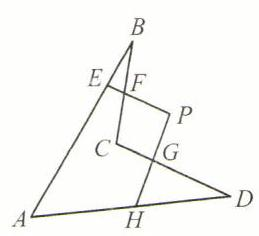
\includegraphics[width=0.2\textwidth]{bodyxb/src/bo_d20aucref24c73anc48g_130_1194_1492_259_236_0.jpg}
    \end{center}

    \xx{平面 ${ABD}$ 内}{直线 ${AC}$ 上}{直线 ${AD}$ 上}{直线 ${BD}$ 上}
    \begin{jieda}
        运用公理 3,可知点 $P$ 在平面 ${ABC}$ 和平面 ${ADC}$ 的交线 ${AC}$ 上
    \end{jieda}
    
    \item 已知平面 $\alpha  \cap$ 平面 $\beta  = l$ ,点 $M \in  \alpha ,N \in  \alpha$ ,且 $P \in  \beta ,P \in  l$ ,又 ${MN} \cap  l$  $= R\left( {R \neq  P}\right)$ ,过 $M,N,P$ 三点所确定的平面记为 $\gamma$ ,则 $\beta  \cap  \gamma$ 等于 \dotfill{(\kh{C})}
    \xx{直线 ${MP}$}{直线 ${NP}$}{直线 ${PR}$}{直线 ${MR}$}
    \begin{jieda}
        $\because \alpha  \cap  \beta  = l,P \in  l.\therefore P \in  \alpha$ . 又, $M,N \in  \alpha$ ,根据公理 2,平面 $\gamma$ 即平面 $\alpha$

        $\therefore \beta  \cap  \gamma  = \beta  \cap  \alpha  = l.M,N,P,R$ 四点中, $P,R \in  l$ 且 $P \neq  R$ (否则 $M,N,P$ 三点共线),故 $\beta  \cap  \gamma  = l =$ 直线 ${PR}$ .
    \end{jieda}
    \item 在正方体 ${ABCD} - {A}_{1}{B}_{1}{C}_{1}{D}_{1}$ 中, $P,Q,R$ 分别是棱 $A{A}_{1},B{B}_{1},D{D}_{1}$ 上的点 (如图).
    \begin{center}
    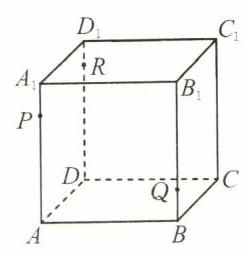
\includegraphics[width=0.2\textwidth]{bodyxb/src/bo_d20aucref24c73anc48g_130_1211_1889_248_253_0.jpg}
    \end{center}
    \begin{enumerate}
        \item 画出过 $P$ 和 $Q$ 两点的直线与底面 ${ABCD}$ 的交点
        \item 画出过 $R$ 和 $Q$ 两点的直线与底面 ${ABCD}$ 的交点
    \end{enumerate}
    \begin{jieda}
        \begin{enumerate}
            \item 在平面 ${A}_{1}{B}_{1}{BA}$ 中,延长 ${PQ},{AB}$ 得到的交点 $S$ 即为所求. 简证: ${AB}$ 是平面 ${A}_{1}{B}_{1}{BA}$ 和平面 ${ABCD}$ 的交线, $S \in$  ${PQ}$ 且 $S \in  {AB} \subset$ 平面 ${ABCD}$ ,故知点 $S$ 为所求交点.
            
            \item 在平面 ${D}_{1}{B}_{1}{BD}$ 中,延长 ${RQ}$ , ${DB}$ 得到的交点 $T$ 即为所求. 简证: ${DB}$ 是平面 ${D}_{1}{B}_{1}{BD}$ 和平面 ${ABCD}$ 的交线, $T \in$  ${RQ}$ 且 $T \in  {DB} \subset$ 平面 ${ABCD}$ ,故知点 $T$ 为所求交点.
        \end{enumerate}
    \end{jieda}
    
    \item 在正方体 ${ABCD} - {A}_{1}{B}_{1}{C}_{1}{D}_{1}$ 中,根据给出的条件,分别画出有关图形 (如图):
    
    \begin{center}
    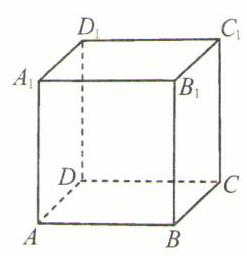
\includegraphics[width=0.2\textwidth]{bodyxb/src/bo_d20aucref24c73anc48g_131_1134_194_247_256_0.jpg}
    \end{center}
    \begin{enumerate}
        \item 过 $B,{A}_{1},{C}_{1}$ 三点的截面
        \item 过 ${B}_{1},A,C$ 三点的截面
        \item 上述两截面的交线
    \end{enumerate}
    \begin{jieda}
        \begin{center}
        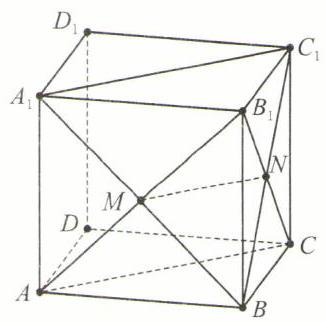
\includegraphics[width=0.2\textwidth]{bodyxb/src/bo_d20cdrf7aajc73bfmvhg_111_1116_1816_326_323_0.jpg}
        \end{center}
        \begin{enumerate}
            \item 如图,连接 $B{A}_{1},{A}_{1}{C}_{1},{C}_{1}B$ ,三角形 ${A}_{1}{C}_{1}B$ 所在平面即为所求. 说明: 根据公理 3 , 三角形 ${A}_{1}{C}_{1}B$ 所在平面与平面 ${A}_{1}{B}_{1}{BA}$ 的交线为 $B{A}_{1}$ ,与 ${A}_{1}{B}_{1}{C}_{1}{D}_{1}$ 的交线为 ${A}_{1}{C}_{1}$ ,与 ${B}_{1}{C}_{1}{CB}$ 的交线为 ${C}_{1}B$ .
            \item 与前一问类似,连接 ${B}_{1}A,{AC},C{B}_{1}$ ,三角形 ${B}_{1}{AC}$ 所在平面即为所求.
            \item 承前两问,记 $B{A}_{1}$ 交 $A{B}_{1}$ 于点 $M,B{C}_{1}$ 交 $C{B}_{1}$ 于点 $N$ ,连接 ${MN}$ ,直线 ${MN}$ 即为所求. 说明: $M,N \in$ 平面 ${A}_{1}{C}_{1}B,M,N \in$ 平面 ${B}_{1}{AC}$ ,根据公理 $3,{MN} =$ 平面 ${A}_{1}{C}_{1}B$  $\cap$ 平面 ${B}_{1}{AC}$ .
        \end{enumerate}
    \end{jieda}
    \item \begin{enumerate}
        \item 已知线段 ${AB}//{CD}$ ,且 ${AB} \cap  \alpha  = E,{CD} \cap  \alpha  = F$ (如图),画出线段 ${AD},{BC}$ 与平面 $\alpha$ 的交点
        \begin{center}
        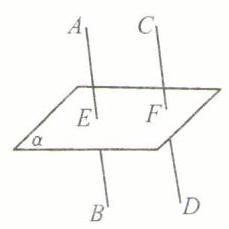
\includegraphics[width=0.2\textwidth]{bodyxb/src/bo_d20aucref24c73anc48g_131_245_857_229_229_0.jpg}
        \end{center}
        \begin{jieda}
            连接 ${EF}$ . 连接 ${AD}$ 与 ${EF}$ 交于点 $G$ ,点 $G$ 即为线段 ${AD}$ 与平面 $\alpha$ 的交点; 连接 ${BC}$ 与 ${EF}$ 交于点 $H$ ,点 $H$ 即为线段 ${BC}$ 与平面 $\alpha$ 的交点. 
            
            说明: 根据公理 2 的推论 3 ,平行直线 ${AB}\text{ 、 }{CD}$ 可确定一个平面,记为 $\beta$ . 根据公理 $3,\alpha  \cap  \beta  = {EF}$ ,且线段 ${AD},{BC}$ 与平面 $\alpha$ 的交点一定在 $\alpha$ 与 $\beta$ 的交线 ${EF}$ 上. $\therefore G = {AD} \cap  {EF},H = {BC} \cap  {EF}$
        \end{jieda}
        \item 已知 $\bigtriangleup {ABC}$ 的边 ${AB}$ , ${BC}$ 与平面 $\alpha$ 分别交于 $P$ , $Q$ 两点(如图),画出直线 ${AC}$ 与平面 $\alpha$ 的交点 $R$ ,并说明理由
        \begin{center}
        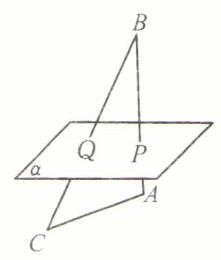
\includegraphics[width=0.2\textwidth]{bodyxb/src/bo_d20aucref24c73anc48g_131_600_823_221_260_0.jpg}
        \end{center}
        \begin{jieda}
            连接 ${QP}$ . 在平面 ${ABC}$ 内,延长 ${QP}$ 与 ${CA}$ ,得到的交点即为 $R$ . 
            
            说明:三角形 ${ABC}$ 所在平面记为 $\beta$ . 根据公理 $3,\alpha  \cap  \beta$  $= {QP}$ ,且 ${CA}$ 与平面 $\alpha$ 的交点一定在 $\alpha$ 与 $\beta$ 的交线 ${QP}$ 上. $\therefore R = {CA} \cap  {QP}$
        \end{jieda}
        \item 在四面体 ${ABCD}$ 中,已知点 $M,N,P$ 分别在棱 ${AD},{BD},{CD}$ 上,点 $S$ 在面 ${ABC}$ 内 (如图),画出线段 ${SD}$ 与过点 $M,N,P$ 的截面的交点
        \begin{center}
        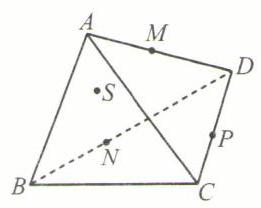
\includegraphics[width=0.2\textwidth]{bodyxb/src/bo_d20aucref24c73anc48g_131_950_872_261_208_0.jpg}
        \end{center}
        \begin{jieda}
            如图,延长 ${AS}$ 与 ${BC}$ 交于点 $E$ ,连接 ${DE}$ , ${NP}$ 交于点 $F$ . 连接 ${MF}$ ,与 ${SD}$ 的交点 $G$ 即为所求. 简证: 根据公理 $3,M,F \in$ 平面 ${MNP},M,F \in$ 平面 ${ADE}$ ,故平面 ${MNP} \cap$ 平面 ${ADE} = {MF}$ ; 线段 ${SD} \subset$ 平面 ${ADE}$ ,故线段 ${SD}$ 与平面 ${MNP}$ 的交点必在平面 ${MNP}$ 与平面 ${ADE}$ 的交线 ${MF}$ 上. $\therefore G = {SD} \cap  {MF}$ .
            
            \begin{center}
            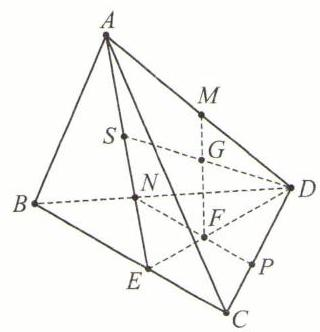
\includegraphics[width=0.2\textwidth]{bodyxb/src/bo_d20cdrf7aajc73bfmvhg_112_1214_291_320_332_0.jpg}
            \end{center}
        \end{jieda}
    \end{enumerate}
    \item \begin{enumerate}
        \item 两个平面把空间分成几个部分？画图表示各种情况
        \begin{jieda}
            3 或 4 部分, 按相交情况分类: \ding{172} 两个平面没有公共点 (交线), 此时空间被分为 3 部分, 俯视图如图甲; \ding{173}两个平面有公共点 (根据公理 3 , 有且只有 1 条交线), 此时空间被分为 4 部分, 俯视图如图乙.
            
            \begin{center}
            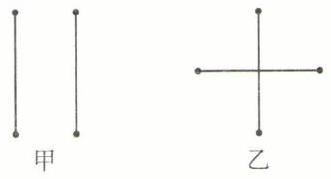
\includegraphics[width=0.2\textwidth]{bodyxb/src/bo_d20cdrf7aajc73bfmvhg_112_553_574_331_179_0.jpg}
            \end{center}
        \end{jieda}
        \item 三个平面把空间分成几个部分？画图表示各种情况
        \begin{jieda}
            4,6,7 或 8 部分,按相交情况分类. 
            \begin{dingautolist}{172}
                \item 三个平面两两不相交,此时空间被分为 4 部分
                \item 两个平面相交,第 3 个平面只与其中 1 个平面相交,共 2 条交线,此时空间被分为 6 部分
                \item 三个平面两两相交,但通过同一条交线,此时空间被分为 6 部分
                \item 三个平面两两相交,产生的 3 条交线没有公共点,此时空间被分为 7 部分
                \item 三个平面两两相交,产生的 3 条交线有同一公共点 (可由公理 3 证明),此时空间被分为 8 部分
            \end{dingautolist}
            \ding{172}$\sim$ \ding{175}的俯视图如图甲、乙、丙、丁,情况，\ding{176} 可参照正方体的底面和两个相邻侧面.

            \begin{center}
            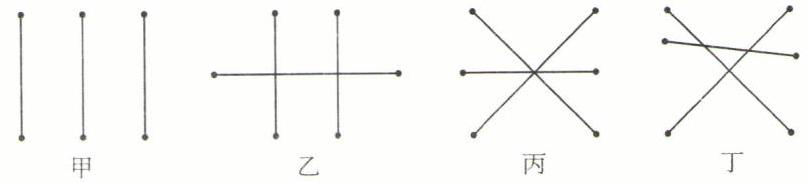
\includegraphics[width=0.6\textwidth]{bodyxb/src/bo_d20cdrf7aajc73bfmvhg_112_455_1089_807_183_0.jpg}
            \end{center}

            \ps \ding{172}两个平面相交,第 3 个平面与这两个平面都不相交,是不可能的,学生在学过两个平面平行的相关知识后很容易证明这点. \ding{173}三个平面两两相交, 但仅有 2 条交线, 也是不可能的, 运用反证法和公理 2 的推论即可证明.
        \end{jieda}
    \end{enumerate}
    \item 在四边形 ${ABCD}$ 中,已知 ${AB}//{CD},{AB},{BC},{AD},{DC}$ (或延长线) 分别与平面 $\alpha$ 相交于点 $E,G,H,F$ (如图). 求证: 点 $E,F,G,H$ 必在同一条直线上
    \begin{center}
    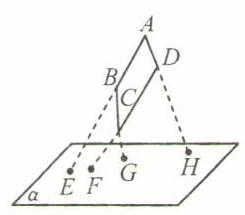
\includegraphics[width=0.2\textwidth]{bodyxb/src/bo_d20aucref24c73anc48g_131_1138_1171_245_215_0.jpg}
    \end{center}
    \begin{jieda}
        证明: $\because {AB}//{CD},\therefore {AB},{CD}$ 确定一个平面 (公理 2 推论 3),记为 $\beta$ . 在平面 ${ABCD}$ 中, ${AB},{BC},{CD},{DA} \subset  \beta$ (公理 1), $\therefore E \in  {AB} \subset  \beta$ ,又 $E \in  \alpha ,\therefore E$ 在 $\alpha$ 与 $\beta$ 的交线上 (公理 3),记交线为 $l$ . 同理, $F,G,H \in  l,\therefore E,F,G,H$ 四点共线.
    \end{jieda}
    \item 求证:
    \begin{enumerate}
        \item 空间不共点且两两相交的四条直线在同一平面上
        \begin{jieda}
            证明: 由题意,这四条直线中,必有 3 条 (记为直线 ${l}_{1},{l}_{2},{l}_{3}$ ) 两两相交且不共点,交点也不在同一直线上,根据公理 2, 这 3 点确定一个平面 (记为 $\alpha$ ). 再根据公理 $1,{l}_{1},{l}_{2},{l}_{3} \subset  \alpha$ . 现记第 4 条直线为 ${l}_{4}$ ,则 ${l}_{4}$ 上至少有 2 点 (与直线 ${l}_{1},{l}_{2}$ , ${l}_{3}$ 的交点)在平面 $\alpha$ 内,根据公理 $1,{l}_{4} \subset  \alpha$ . 故四线共面,证毕.
        \end{jieda}
        \item 相交于一点的一组直线如果与不过该公共点的一条直线都相交, 那么这组直线在同一平面上
        \begin{jieda}
            证明:设这组直线为 ${l}_{1},{l}_{2},\cdots ,{l}_{n}$ 有公共点 $P$ ,且直线 ${l}_{i} \cap  l = {P}_{i} \neq  P\left( {i = 1,2,\cdots ,n}\right)$ . 不妨先取 ${l}_{1},{l}_{2},l$ ,由题意,这 3 条直线两两相交,且 ${P}_{1},{P}_{2},P$ 是不共线的 3 点,根据公理 2,这 3 点确定一个平面 (记为 $\alpha$ ). 再根据公理 $1,{l}_{1},{l}_{2},l \subset$  $\alpha$ . 又 $P \in  {l}_{i},{P}_{i} \in  {l}_{i},P \in  \alpha ,{P}_{i} \in  l \subset  \alpha$ ,根据公理 $1,{l}_{i} \subset  \alpha \left( {i = 1,2,\cdots ,n}\right)$ . 证毕.
        \end{jieda}
    \end{enumerate}
    \item 已知一条直线和四条平行直线都相交, 求证: 这五条直线在同一平面上.
    \begin{jieda}
        设平行直线为 ${l}_{1}//{l}_{2}//{l}_{3}//{l}_{4}$ ,且直线 ${l}_{i} \cap  l = {P}_{i}\left( {i = 1,2,3,4}\right)$ . 不妨先取 ${l}_{1},{l}_{2},l$ ,根据公理 2 的推论 $3,{l}_{1},{l}_{2}$ 确定一个平面 (记为 $\alpha$ ). 再根据公理 $1,l \subset  \alpha$ . 同理, ${l}_{2},{l}_{3},l$ 也共面,记为 ${\alpha }^{\prime }$ . 若 $\alpha  \neq  {\alpha }^{\prime }$ ,则有 ${l}_{2} \subset  \alpha ,{l}_{2} \subset  {\alpha }^{\prime },l \subset  \alpha ,l \subset  {\alpha }^{\prime }$ ,即 $\alpha$ 与 ${\alpha }^{\prime }$ 的交线为 ${l}_{2}$ 或 $l$ ,而 ${l}_{2} \neq  l$ ,这显然与公理 3 矛盾,因此 $\alpha  = {\alpha }^{\prime }$ . 以此类推, ${l}_{1},{l}_{2},{l}_{3},{l}_{4},l$ 五条直线共面. 证毕.
    \end{jieda}
    \item 在正方体 ${ABCD} - {A}_{1}{B}_{1}{C}_{1}{D}_{1}$ 中,记 ${A}_{1}C$ 与平面 ${AB}{C}_{1}{D}_{1}$ 交于点 $Q$ (如图),求证:点 $B,Q,{D}_{1}$ 共线.
    \begin{center}
    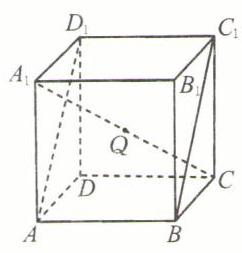
\includegraphics[width=0.2\textwidth]{bodyxb/src/bo_d20aucref24c73anc48g_131_1141_1551_242_253_0.jpg}
    \end{center}
    \begin{jieda}
        $B,{D}_{1} \in$ 平面 ${AB}{C}_{1}{D}_{1},B,{D}_{1} \in$ 平面 ${BC}{D}_{1}{A}_{1},\therefore$ 这两个平面的交线是 $B{D}_{1}$ (公理 3). 又 $Q \in  {A}_{1}C \subset$ 平面 ${BC}{D}_{1}{A}_{1}$ , $Q \in$ 平面 ${AB}{C}_{1}{D}_{1},\therefore$ 点 $Q$ 在平面 ${BC}{D}_{1}{A}_{1}$ 与平面 ${AB}{C}_{1}{D}_{1}$ 的交线 $B{D}_{1}$ 上 (公理 3), $\therefore B,Q,{D}_{1}$ 三点共线. 证毕.
    \end{jieda}
\end{enumerate}

\section*{二、直线与直线的位置关系}

\subsection*{【典型题型和解题技巧】}

1. 异面直线所成角的计算.

两条异面直线所成角的求解, 既是本单元学习的重点, 也是难点.

求两条异面直线所成的角, 主要有两种方法.

(1)平移. 所谓平移,就是平移两条异面直线中的一条或两条,使之转化为两条相交直线所夹的角.

\textbf{例 1} 在正四面体 ${ABCD}$ (四个面是全等的等边三角形的四面体) 中, 已知 $E$ 是棱 ${BC}$ 的中点,求异面直线 ${AE}$ 和 ${BD}$ 所成角的余弦值.

\textbf{解} 

\begin{center}
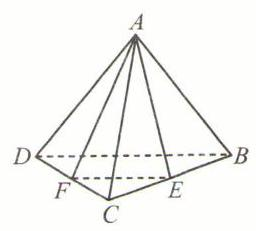
\includegraphics[width=0.2\textwidth]{bodyxb/src/bo_d20aucref24c73anc48g_132_1190_654_256_231_0.jpg}
\end{center}

如图，取 ${CD}$ 的中点 $F$ ,连接 ${EF}$ ,则 ${EF}//{BD}$ ,于是 $\angle {AEF}$ (或其补角) 就是异面直线 ${AE}$ 和 ${BD}$ 所成的角.

连接 ${AF}$ ,在 $\bigtriangleup {AEF}$ 中,令 ${AB} = 2$ ,则 ${AE} = {AF} = \sqrt{3}$ , ${EF} = 1$ ,于是由余弦定理可得, $\cos \angle {AEF} = \dfrac{\sqrt{3}}{6}$ ,故异面直线 ${AE}$ 和 ${BD}$ 所成角的余弦值为 $\dfrac{\sqrt{3}}{6}$ .

\textbf{例 2} 已知正四面体 ${ABCD}$ ,求异面直线 ${AB}$ 和 ${CD}$ 所成角的大小.

\textbf{解}

\begin{center}
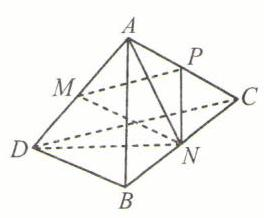
\includegraphics[width=0.2\textwidth]{bodyxb/src/bo_d20aucref24c73anc48g_132_1183_1158_264_218_0.jpg}
\end{center}

如图，分别取 ${AC},{AD},{BC}$ 的中点 $P,M,N$ ,连接 ${PM},{PN}$ . 由三角形中位线性质得, ${PN}//{AB},{PM}//{CD}$ ,于是 $\angle {MPN}$ (或其补角) 就是异面直线 ${AB}$ 和 ${CD}$ 所成的角.



连接 ${MN},{DN}$ . 设 ${AB} = 2$ ,则 ${PM} = {PN} = 1$ ,而 ${AN} = {DN} = \sqrt{3}$ ,由 $M$ 是 ${AD}$ 的中点,得 ${MN}\bot {AD},{AM} = 1$ . 计算得 ${MN} = \sqrt{2}$ ,故 $\angle {MPN} = {90}^{ \circ  }$ , 即异面直线 ${AB}$ 和 ${CD}$ 所成角为 ${90}^{ \circ  }$ .

(2) 补形.

\textbf{例 3} 在长方体 ${ABCD} - {A}^{\prime }{B}^{\prime }{C}^{\prime }{D}^{\prime }$ 中,已知 ${AB} = a,{BC} = b,A{A}^{\prime } = c\left( {a > b}\right)$ ,求异面直线 ${D}^{\prime }B$ 和 ${AC}$ 所成角的余弦值.

\textbf{解}

\begin{center}
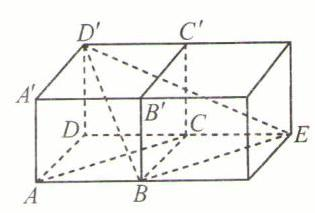
\includegraphics[width=0.2\textwidth]{bodyxb/src/bo_d20aucref24c73anc48g_132_1135_1681_315_213_0.jpg}
\end{center}

在长方体的一旁, 补上一个全等的长方体， 则 ${BE}$ 与 ${AC}$ 平行且相等, $\angle {D}^{\prime }{BE}$ (或其补角) 即 ${D}^{\prime }B$ 和 ${AC}$ 所成的角.

$\because {D}^{\prime }B = \sqrt{{a}^{2} + {b}^{2} + {c}^{2}},{BE} = \sqrt{{a}^{2} + {b}^{2}},{D}^{\prime }E = \sqrt{4{a}^{2} + {c}^{2}}$ ,

$\therefore \cos \angle {D}^{\prime }{BE} = \dfrac{{D}^{\prime }{B}^{2} + B{E}^{2} - {D}^{\prime }{E}^{2}}{2 \cdot  {D}^{\prime }B \cdot  {BE}} = \dfrac{-{a}^{2} + {b}^{2}}{\sqrt{\left( {{a}^{2} + {b}^{2}}\right) \left( {{a}^{2} + {b}^{2} + {c}^{2}}\right) }} < 0$

$\therefore {D}^{\prime }B$ 与 ${AC}$ 所成角的余弦值为 $\dfrac{{a}^{2} - {b}^{2}}{\sqrt{\left( {{a}^{2} + {b}^{2}}\right) \left( {{a}^{2} + {b}^{2} + {c}^{2}}\right) }}$ .

注意 本例也可用 “平移”的方法求解 (平移 ${D}^{\prime }B$ 或平移 ${AC}$ ),读者不妨试一试.

2. 异面直线的证明.

\textbf{例 4} 求证: 空间四边形的两条对角线是异面直线.

\begin{center}
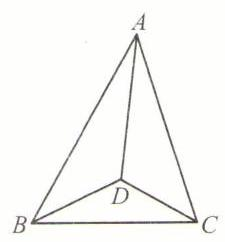
\includegraphics[width=0.2\textwidth]{bodyxb/src/bo_d20aucref24c73anc48g_133_1144_261_225_242_0.jpg}
\end{center}

\textbf{证明} 

证法一

假设空间四边形 ${ABCD}$ 的对角线 ${AC},{BD}$ 不是异面直线,则 ${AC},{BD}$ 共面于 $\alpha$ ,因此点 $A,B,C,D$ 均在平面 $\alpha$ 内,这与已知 “ ${ABCD}$ 是空间四边形(四个顶点不在同一平面上)”相矛盾.

故假设错误,因此 ${AC},{BD}$ 是异面直线.

证法二 

因为 ${CD} \subset$ 平面 ${BCD}$ , $A$ 不在平面 ${BCD}$ 上, $B$ 在平面 ${BCD}$ 上且不在直线 ${CD}$ 上,由异面直线判定定理知 ${AB}$ 与 ${CD}$ 是异面直线.

注意 证明两条直线是异面直线,通常有两种方法. 

证法一是反证法. 例如:要证明直线 ${AB}$ , ${CD}$ 异面,首先可假设 ${AB}$ , ${CD}$ 不异面,则 ${AB}$ , ${CD}$ 共面于 $\alpha \cdots$

证法二是利用异面直线判定定理.

\subsection*{【训练题】}

\begin{center}  \textbf{(A)} \end{center}
\begin{enumerate}
    \item 两条异面直线是指\dotfill{(\kh{D})}
    \xx{空间两条没有公共点的直线}{平面上一直线与这平面外的一条直线}{分别在两个平面上的两条直线}{不同在任何一个平面上的两条直线}
    \begin{jieda}
        选项 (D) 是异面直线的定义. 其余 3 个选项的反例如下:对于选项 (A),两条平行直线；对于选项 (B),正方体 ${ABCD} - {A}^{\prime }{B}^{\prime }{C}^{\prime }{D}^{\prime }$ 中,平面 ${ABCD}$ 内的直线 ${AB}$ 与平面外的直线 ${A}^{\prime }{B}^{\prime }$ ; 对于选项 (D),正方体 ${ABCD} - {A}^{\prime }{B}^{\prime }{C}^{\prime }{D}^{\prime }$ 中,平面 ${ABCD}$ 内的直线 ${AB}$ 与平面 ${A}^{\prime }{B}^{\prime }{C}^{\prime }{D}^{\prime }$ 内的直线 ${A}^{\prime }{B}^{\prime }$
    \end{jieda}
    \item 已知平面 $\alpha  \cap$ 平面 $\beta  =$ 直线 $c$ ,直线 $a \subset  \alpha ,a//c$ ,直线 $b \subset  \beta$ ,且 $b$ 与 $c$ 相交,则 $a$ 和 $b$ 的位置关系是\dotfill{(\kh{C})}
    \xx{平行}{相交}{异面}{上述三种情况都有可能}
    \begin{jieda}
        符合异面直线判定定理的条件
    \end{jieda}
    \item 已知 $a,b$ 是异面直线,直线 $c//a$ ,那么 $c$ 与 $b$ \dotfill{(\kh{C})}
    \xx{一定是异面直线}{一定是相交直线}{不可能是平行直线}{不可能是相交直线}
    \begin{jieda}
        根据公理 4 ; 空间内,平行于同一直线的两直线互相平行. $c//b$ 是不可能的. 直线 $c$ 和 $b$ 异面和相交均有可能,例如,正方体 ${ABCD} - {A}^{\prime }{B}^{\prime }{C}^{\prime }{D}^{\prime }$ 中,取 $a = {AB},b = {A}_{1}{D}_{1},c = {CD}$ 时, $b$ 与 $c$ 异面; $c = {D}_{1}{C}_{1}$ 时, $b$ 与 $c$ 相交. 因此只有选项 (C) 正确.
    \end{jieda}
    \item 若 $a,b$ 是异面直线, $b,c$ 也是异面直线,则 $a,c$ 的位置关系是\dotfill{(\kh{A})}
    \xx{相交、平行或异面}{相交或平行}{异面}{平行或异面}
    \begin{jieda}
        以正方体 ${ABCD} - {A}^{\prime }{B}^{\prime }{C}^{\prime }{D}^{\prime }$ 为例,取 $a = {AB},b = {A}_{1}{D}_{1}$ ,若 $c = {BD}$ ,则 $a$ , $c$ 相交；若 $c = {CD}$ ,则 $a$ , $c$ 平行；若 $c =$  $C{C}_{1}$ ,则 $a,c$ 异面.
    \end{jieda}
    \item 经过空间一点 $A$ ,作与直线 $l$ 成 $\dfrac{\pi }{3}$ 角的直线共有 \dotfill{(\kh{D})}
    \xx{2 条}{3 条}{4 条}{无数条}
    \begin{jieda}
        若直线 $l$ 不经过点 $A$ ,则过 $A$ 点作直线 ${l}^{\prime }//l$ ,若直线 $l$ 经过点 $A$ ,取 ${l}^{\prime } = l$ . 在空间中,任作一条过点 $A$ 且与直线 ${l}^{\prime }$ 成 $\dfrac{\pi }{3}$ 角的直线,再将该直线绕着直线 ${l}^{\prime }$ 旋转一周 (得到两个对顶的圆锥),即得到无数条符合要求的直线.
    \end{jieda}
    \item 已知异面直线 $a$ 与 $b$ 满足 $a \subset  \alpha ,b \subset  \beta$ ,且 $\alpha  \cap  \beta  = l$ ,则直线 $l$ 与 $a,b$ 的位置关系一定是\dotfill{(\kh{B})}
    \xx{$l$ 与 $a,b$ 都相交}{$l$ 至少与 $a,b$ 中的一条相交}{$l$ 至多与 $a,b$ 中的一条相交}{$l$ 至少与 $a,b$ 中的一条平行}
    \begin{jieda}
        由于 $l \subset  \alpha ,l \subset  \beta$ ,若 $l$ 与直线 $a,b$ 均无交点,则 $a//l,b//l$ ,根据公理 $4,a//b$ ,这与 $a,b$ 是异面直线矛盾,故 $l$ 至少与 $a,b$ 中的一条相交,选项 (B) 正确,而选项 (C) 错误. 以正方体 ${ABCD} - {A}^{\prime }{B}^{\prime }{C}^{\prime }{D}^{\prime }$ 为例,取 $\alpha  =$ 平面 ${ABCD},\beta  =$ 平面 ${AD}{D}^{\prime }{A}^{\prime }$ ,则 $l = {AD}$ ,选项 (A) 反例: 取 $a = {AB},b = {A}^{\prime }{D}^{\prime }$ ; 选项 (D) 的反例: 取 $a = {AB},b = {A}^{\prime }D$
    \end{jieda}
    \item 有以下三个命题:\ding{172}若两条直线和第三条直线成等角,则这两条直线互相平行；\ding{173}若两条直线都和第三条直线垂直,则这两条直线互相平行；\ding{174}若两条直线都和第三条直线平行, 则这两条直线互相平行. 其中不正确的个数为\dotfill{(\kh{C})}
    \xx{0}{1}{2}{3}
    \begin{jieda}
        \ding{174}是公理4，\ding{172}\ding{173}均有异面的可能
    \end{jieda}
    \item 在正方体 ${ABCD} - {A}_{1}{B}_{1}{C}_{1}{D}_{1}$ 中,
    \begin{enumerate}
        \item 各个面的对角线所在直线中,与 $A{B}_{1}$ 异面且所成角为 ${60}^{ \circ  }$ 的直线有\blkda{4}条
        \begin{jieda}
            各个面总计 12 条对角线,与 $A{B}_{1}$ 成异面直线的是 $B{C}_{1},{A}_{1}D,{A}_{1}{C}_{1},{BD},{D}_{1}C$ ,通过平移,可知前 4 条与 $A{B}_{1}$ 成 ${60}^{ \circ  }$ 角,而 ${D}_{1}C$ 与 $A{B}_{1}$ 成 ${45}^{ \circ  }$ 角,因此共 4 条满足题意.
        \end{jieda}
        \item 若 $E$ , $F$ 分别为棱 ${A}_{1}{B}_{1}$ , $B{B}_{1}$ 的中点,则 ${AE}$ 和 ${CF}$ 所成角的余弦值为\blkda{$\dfrac{2}{5}$}
        \begin{jieda}
            取平面$CC_1D_1D$的中点$O$，连接$EO$，$EO // CF$，则$\angle{AEO}$即为异面直线所成角（或其补角），根据余弦定理可知$cos\angle{AEO} = \dfrac{5+5-6}{10} = \dfrac{2}{5}$
        \end{jieda}
        \item 若 $G$ 为 ${CD}$ 的中点,则异面直线 ${B}_{1}C$ 与 ${AG}$ 所成角的正弦值是\blkda{$\dfrac{\sqrt{15}}{5}$}
        \begin{jieda}
            取$AB$中点$H$，连接$CH$，$CH // AG$，故$\angle{B_1CH}$即为异面直线所成角（或其补角），根据余弦定理可知$cos\angle{B_1CH} = \dfrac{5+8-5}{4\sqrt{10}} = \dfrac{\sqrt{10}}{5}$，故$sin\angle{B_1CH} = \dfrac{\sqrt{15}}{5}$
        \end{jieda}
    \end{enumerate}
    \item 在正方体 ${ABCD} - {A}_{1}{B}_{1}{C}_{1}{D}_{1}$ 中,
    \begin{enumerate}
        \item 若 $F$ , $G$ 分别是棱 $B{B}_{1}$ , ${DC}$ 的中点,则 ${AF}$ 与 ${D}_{1}G$ 所成角为\blkda{${90}^{ \circ  }$}
        \begin{jieda}
            取$CC_1$中点$H$，$DH // AF$，设$D_1G$与$DH$交于$M$，则$\angle{DMD_1}$即为异面直线所成角（或其补角），根据勾股定理可知$\angle{DMD_1} = 90^{\circ}$
        \end{jieda}
        \item 已知 $E,F$ 分别是棱 $B{B}_{1},C{C}_{1}$ 的中点,则异面直线 ${AE},{BF}$ 所成角的余弦值等于\blkda{$\dfrac{1}{5}$}
        \begin{jieda}
            取$DD_1$中点$H$，$AH // BF$，则$\angle{HAE}$即为异面直线所成角（或其补角），根据余弦定理可知$cos\angle{HAE} = \dfrac{5+5-8}{10} = \dfrac{1}{5}$
        \end{jieda}
    \end{enumerate}
    \item  在长方体 ${ABCD} - {A}_{1}{B}_{1}{C}_{1}{D}_{1}$ 中,
    
    \begin{center}
    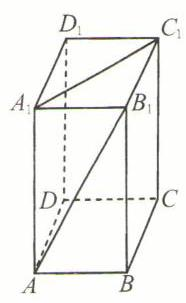
\includegraphics[width=0.2\textwidth]{bodyxb/src/bo_d20aucref24c73anc48g_134_1256_820_186_303_0.jpg}
    \end{center}
    \begin{enumerate}
        \item 若棱 $B{B}_{1} = {BC} = 1,{AB} = \sqrt{3}$ ,则 $A{D}_{1}$ 与 ${BC}$ 所成角等于\blkda{${45}^{ \circ  }$}, $C{D}_{1}$ 与 ${AB}$ 所成角等于\blkda{${30}^{ \circ  }$}, $C{D}_{1}$ 与 ${A}_{1}D$ 所成角的正弦值等于\blkda{$\dfrac{\sqrt{14}}{4}$}
        \begin{jieda}
            ${BC} \bot  {AD}$ ,故 $A{D}_{1}$ 与 ${BC}$ 所成角为 $\angle {D}_{1}{AD} = \arctan \dfrac{{D}_{1}D}{AD} = \arctan \dfrac{1}{1} = {45}^{ \circ  }$
            
            ${AB} \bot  {CD}$ ,故 $C{D}_{1}$ 与 ${AB}$ 所成角为 $\angle {D}_{1}{CD} = \arctan \dfrac{{D}_{1}D}{CD} = \arctan \dfrac{1}{\sqrt{3}} = {30}^{ \circ  }$
            
            易证四边形 ${A}_{1}{B}_{1}{CD}$ 是平行四边形,故 ${A}_{1}D\bot {B}_{1}C$，不难求得 ${B}_{1}C = \sqrt{2},{D}_{1}C = {D}_{1}{B}_{1} = 2,C{D}_{1}$ 与 ${A}_{1}D$ 所成角为 $\angle {D}_{1}C{B}_{1},\cos \angle {D}_{1}C{B}_{1} = \dfrac{C{D}_{1}^{2} + C{B}_{1}^{2} - {B}_{1}{D}_{1}^{2}}{2 \cdot  C{D}_{1} \cdot  C{B}_{1}} = \dfrac{\sqrt{2}}{4}$ ,故 $\sin \angle {D}_{1}{CD} = \dfrac{\sqrt{14}}{4}.$
        \end{jieda}
        \item 若 $\angle {BA}{B}_{1} = \angle {B}_{1}{A}_{1}{C}_{1} = {60}^{ \circ  }$，则 $A{A}_{1}$ 与 ${B}_{1}C$ 所成角的余弦值等于\blkda{$\dfrac{\sqrt{2}}{2}$}, ${B}_{1}C$ 与 ${A}_{1}{C}_{1}$ 所成角的余弦值等于\blkda{$\dfrac{\sqrt{6}}{4}$}
        \begin{jieda}
            $\angle{BB_1C}$即为异面直线所成角（或其补角） $\angle B{B}_{1}C = {45}^{ \circ  },\cos \angle B{B}_{1}C = \dfrac{\sqrt{2}}{2}$ .
            
            $\angle{DA_1C_1}$即为异面直线所成角（或其补角） $\cos \angle DA_1C_1 = \dfrac{6+4-4}{4\sqrt{6}} = \dfrac{\sqrt{6}}{4}$ .
        \end{jieda}
        \item 若底面边长 ${AB} = {BC} = 3$ ,棱 $A{A}_{1} = 4$ ,则异面直线 $A{B}_{1}$ 与 ${A}_{1}D$ 所成角的余弦值等于\blkda{$\dfrac{16}{25}$}
        \begin{jieda}
            $\angle{AB_1C}$即为异面直线所成角（或其补角） $\cos \angle AB_1C = \dfrac{25+25-18}{50} = \dfrac{16}{25}$ 
        \end{jieda}
    \end{enumerate}
    \clearpage
    \item 在四面体 ${ABCD}$ 中,
    \begin{enumerate}
        \item 若棱 ${AB} = {CD} = 2,E,F$ 分别是棱 ${AC},{BD}$ 的中点,且 ${EF} = \sqrt{3}$ ,则 ${AB}$ 与 ${CD}$ 所成角等于\blkda{$60^\circ$}
        \begin{jieda}
            取$BC$中点$G$，连接$EG, FG$，$\angle{EGF}$即为异面直线所成角（或其补角），$\cos \angle EGF = \dfrac{1+1-3}{2} = -\dfrac{1}{2}$，故异面直线所成角为$60^\circ$
        \end{jieda}
        \item 若 ${AC}$ 与 ${BD}$ 所成角为 ${60}^{ \circ  }$ ,且 ${AC} = {BD} = a$ ,则连接 ${AB},{BC},{CD},{DA}$ 这四条棱的中点所得四边形的面积等于\blkda{$\dfrac{\sqrt{3}}{8}{a}^{2}$}
        \begin{jieda}
            根据几何关系可知${AB},{BC},{CD},{DA}$ 这四条棱的中点所得四边形为边长为$\dfrac{a}{2}$的菱形，该菱形的的内角即异面直线所成角（或其补角），故其面积$S = \dfrac{1}{2}\times \dfrac{a}{2} \times \dfrac{\sqrt{3}a}{2} = \dfrac{\sqrt{3}}{8}{a}^{2}$
        \end{jieda}
    \end{enumerate}
    \item 求证:如果一条直线和两平行线中的一条垂直,那么它也和另一条垂直(本命题今后可作定理用)
    \begin{jieda}
        将命题写为: 若 ${l}_{1}//{l}_{2}$ ,且 $l \bot  {l}_{1}$ ,求证: $l \bot  {l}_{2}$ .
        
        证明：不论 ${l}_{1},{l}_{2},l$ 是否在同一平面,均可在直线 $l$ 上取一点 $P$ ,且 $P \notin  {l}_{1},P \notin  {l}_{2}$ . 过点 $P$ ,作直线 ${l}_{3}//{l}_{1}$ ,则 $l\bot {l}_{3}$ (异面直线所成角的定义). 根据公理 $4,{l}_{2}//{l}_{3}$ ,在 ${l}_{2}$ 和 ${l}_{3}$ 确定的平面中,过点 $P$ 且与 ${l}_{2}$ 平行的直线有且只有 ${l}_{3}$ 一条,所以 $l \bot$  ${l}_{2}$ (异面直线所成角的定义). 证毕.
    \end{jieda}
    \item 在正方体 ${ABCD} - {A}_{1}{B}_{1}{C}_{1}{D}_{1}$ 中,已知 $E$ 为棱 ${CD}$ 的中点 (如图),求 ${AE}$ 和 ${B}_{1}C$ 所成角的余弦值.
    \begin{jieda}
        取$AB$中点$F$，连接$CF$，$\angle{B_1CF}$即为异面直线所成角（或其补角），$\cos \angle B_1CF = \dfrac{5+8-5}{4\sqrt{10}} = \dfrac{\sqrt{10}}{5}$
    \end{jieda}
    
    \begin{center}
    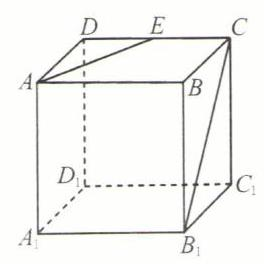
\includegraphics[width=0.2\textwidth]{bodyxb/src/bo_d20aucref24c73anc48g_134_663_1821_264_264_0.jpg}
    \end{center}
    \item 已知 $E,F,G,H$ 顺次是空间四边形 ${ABCD}$ 各边的中点 (如图).
    
    \begin{center}
    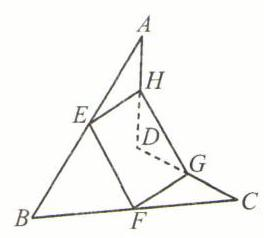
\includegraphics[width=0.2\textwidth]{bodyxb/src/bo_d20aucref24c73anc48g_135_1107_146_264_238_0.jpg}
    \end{center}
    \begin{enumerate}
        \item 求证: ${EFGH}$ 为平行四边形
        \item 如果 ${AC} = {BD}$ ,那么 ${EFGH}$ 是什么四边形？
        \item 如果 ${AC} \bot  {BD}$ ,那么 ${EFGH}$ 是什么四边形？
        \item 如果 ${AC} = {BD}$ ,且 ${AC}\bot {BD}$ ,那么 ${EFGH}$ 是什么四边形？
        \item 若对角线 ${BD} = 2,{AC} = 4$ ,求 $E{G}^{2} + H{F}^{2}$ 的值.
    \end{enumerate}
    \begin{jieda}
        \begin{enumerate}
            \item 证明: 连接 ${AC},{BD}$ . 运用三角形的中位线定理,在 $\bigtriangleup {ABC}$ 中, ${EF}//{AC},{EF} = \dfrac{1}{2}{AC}$ ; 在 $\bigtriangleup {ADC}$ 中, ${HG}//{AC},{HG} =$  $\dfrac{1}{2}{AC}$ . 由公理 4, ${EF}//{HG}$ , ${EFGH}$ 是平面图形,又由 ${EF} = {HG}$ ,故 ${EFGH}$ 是平行四边形. 证毕. (同理, ${EH}//{GF}//$  $\left. {{BD},{EH} = {GF} = \dfrac{1}{2}{BD}}\right)$
            \item 此时, ${EFGH}$ 四边边长相等,故为菱形.
            \item 此时, ${EH}\bot {EF}$ ,故为矩形.
            \item 结合前 2 小问,此时 ${EFGH}$ 为正方形.
            \item $E{G}^{2} + H{F}^{2} = 2\left( {E{H}^{2} + E{F}^{2}}\right)  = \dfrac{1}{2}\left( {B{D}^{2} + A{C}^{2}}\right)  = {10}$ .
            \ps 第(5)问利用了如下结论:平行四边形对角线的平方和,等于四边的平方和.
        \end{enumerate}
    \end{jieda}
\end{enumerate}

\begin{center}  \textbf{(B)} \end{center}
\begin{enumerate}
    \item 分别和两条异面直线都相交的两直线一定是\dotfill{(\kh{A})}
    \xx{不平行的直线}{不相交的直线}{相交直线或平行直线}{既不相交又不平行的直线}
    \begin{jieda}
        如果和两条异面直线都相交的两直线平行, 由于两平行直线可确定一个平面, 根据公理 1, 推知这两条异面直线在同一平面内,矛盾,故选项 $A$ 正确,选项 $C$ 错误. 以正方体 ${ABCD} - {A}^{\prime }{B}^{\prime }{C}^{\prime }{D}^{\prime }$ 为例, ${AB}$ 和 ${A}^{\prime }{D}^{\prime }$ 是两条异面直线,与它们都相交的两直线 $A{A}^{\prime },A{D}^{\prime }$ 相交,而 $A{A}^{\prime },B{D}^{\prime }$ 异面,故选项 $B,D$ 均错误.
    \end{jieda}
    \item 在正方体 ${ABCD} - {A}_{1}{B}_{1}{C}_{1}{D}_{1}$ 中,各面对角线所在的直线中与 ${B}_{1}D$ 成异面直线的条数是\dotfill{(\kh{D})}
    \xx{3}{4}{5}{6}
    \begin{jieda}
        各个面总计 12 条对角线,首先排除从点 ${B}_{1}$ 或点 $D$ 出发的 6 条,其余 6 条可使用异面直线判定定理 (平面外一点与平面内一点的连线,和平面内不经过该点的直线是异面直线),观察对角线、对角线所在的侧面和 ${B}_{1}D$ ,不难判定剩余 6 条都与 ${B}_{1}D$ 异面.
    \end{jieda}
    \item 正方体的两条体对角线相交, 其夹角的正弦值等于 \dotfill{(\kh{C})}
    \xx{$\dfrac{\sqrt{2}}{2}$}{$\dfrac{1}{3}$}{$\dfrac{2\sqrt{2}}{3}$}{$\dfrac{\sqrt{10}}{10}$}
    \begin{jieda}
        设正方体棱长为 1 . 正方体共有 4 条体对角线,任意两条都共面,且是长、宽分别为 $\sqrt{2}$ 、 1 的矩形的对角线. 对角线长 $\sqrt{3}$ ,且两条对角线分矩形为 4 个相等面积的三角形,设对角线所成角为 $\theta ,\therefore 4 \cdot  \dfrac{1}{2} \cdot  {\left( \dfrac{\sqrt{3}}{2}\right) }^{2} \cdot  \sin \theta  = \sqrt{2} \cdot  1$ ,
        $\therefore \sin \theta  = \dfrac{2\sqrt{2}}{3}$ (也可用余弦定理结合三角恒等式求解).
    \end{jieda}
    \item 在正方体 ${EFGH} - {E}^{\prime }{F}^{\prime }{G}^{\prime }{H}^{\prime }$ 中, $F{G}^{\prime }$ 与 ${EG}$ 所成的角等于 \dotfill{(\kh{B})}
    \xx{${45}^{ \circ  }$}{${60}^{ \circ  }$}{${90}^{ \circ  }$}{${120}^{ \circ  }$}
    \begin{jieda}
        易证 ${EF}{G}^{\prime }{H}^{\prime }$ 是平行四边形,故 $E{H}^{\prime }//F{G}^{\prime }$ . 而 $\bigtriangleup {EG}{H}^{\prime }$ 是等边三角形,故 $F{G}^{\prime }$ 与 ${EG}$ 所成的角为 $\angle {GE}{H}^{\prime } = {60}^{ \circ  }$ .
    \end{jieda}
    \item 在正方体 ${ABCD} - {A}_{1}{B}_{1}{C}_{1}{D}_{1}$ 中,已知 $P$ 为 ${AB}$ 的中点, $Q$ 为 ${BC}$ 的中点, $R$ 为 ${A}_{1}{D}_{1}$ 的中点, $S$ 为 $C{C}_{1}$ 的中点,则下面四对直线中不成异面直线的是\dotfill{(\kh{B})}
    \xx{${AR}$ 与 ${A}_{1}P$}{${A}_{1}P$ 与 ${C}_{1}Q$}{${C}_{1}Q$ 与 ${DS}$}{${DS}$ 与 ${AR}$}
    \begin{jieda}
        对于选项 $B,{A}_{1}P$ 和 ${C}_{1}Q$ 共面,证明如下: 延长 ${B}_{1}B$ 至 $T$ ,使得 ${BT} = {B}_{1}B$ . 连接 $T{A}_{1}$ ,交 ${AB}$ 于 ${P}^{\prime }$ . 不难证明 $\bigtriangleup {TB}{P}^{\prime }\cong \bigtriangleup T{B}_{1}{A}_{1},\therefore {P}^{\prime }$ 是 ${AB}$ 的中点,即与点 $P$ 重合, $\therefore T,P,{A}_{1}$ 三点共线. 同理,连接 $T{C}_{1},T,Q,{C}_{1}$ 三点共线. 由公理 2 的推论 2 和公理 1,可知 ${A}_{1}P$ 和 ${C}_{1}Q$ 共面. 
        
        对于其余选项,使用异面直线判定定理 (平面外一点与平面内一点的连线,和平面内不经过该点的直线是异面直线),有:对于选项 $A$ ,观察平面 ${AB}{B}_{1}{A}_{1}$ 及其内的直线 ${A}_{1}P$ ,以及 ${AR}$ ,可知 ${AR}$ 与 ${A}_{1}P$ 异面; 对于选项 $C$ ,观察平面 ${BC}{C}_{1}{B}_{1}$ 及其内的直线 ${C}_{1}Q$ ,以及 ${DS}$ ,可知 ${DS}$ 与 ${C}_{1}Q$ 异面; 对于选项 $D$ ,观察平面 ${AD}{D}_{1}{A}_{1}$ 及其内的直线 ${AR}$ ,以及 ${DS}$ ,可知 ${DS}$ 与 ${AR}$ 异面.
    \end{jieda}
    \item 用 “补形法”解以下各题:
    \fourtu{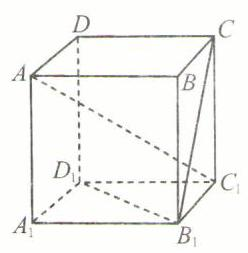
\includegraphics[width=0.9\textwidth]{bodyxb/src/bo_d20aucref24c73anc48g_135_94_1838_248_253_0.jpg}}{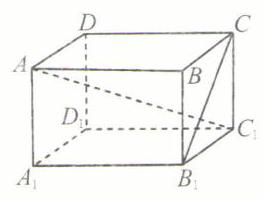
\includegraphics[width=0.9\textwidth]{bodyxb/src/bo_d20aucref24c73anc48g_135_435_1892_265_199_0.jpg}}{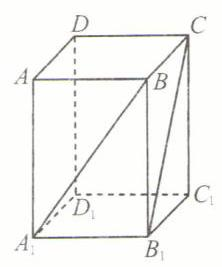
\includegraphics[width=0.9\textwidth]{bodyxb/src/bo_d20aucref24c73anc48g_135_792_1818_222_267_0.jpg}}{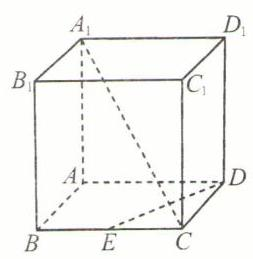
\includegraphics[width=0.9\textwidth]{bodyxb/src/bo_d20aucref24c73anc48g_135_1107_1825_253_259_0.jpg}}
    \begin{enumerate}
        \item 在正方体 ${ABCD} - {A}_{1}{B}_{1}{C}_{1}{D}_{1}$ 中,求 $A{C}_{1}$ 和 ${B}_{1}{D}_{1}$ 所成的角
        \begin{jieda}
            在正方体右侧,补上一个全等的正方体,此时点 ${B}_{1}$ 移动到点 $E$，${C}_{1}E // {D}_{1}{B}_{1}$. 设正方体棱长为 1,则 ${C}_{1}A = \sqrt{3}$ , ${C}_{1}E = \sqrt{2},{AE} = \sqrt{{A}_{1}{A}^{2} + {A}_{1}{E}^{2}} = \sqrt{5}$ ,由勾股定理的逆定理,知 $A{C}_{1}$ 和 ${B}_{1}{D}_{1}$ 所成的角即为 $\angle A{C}_{1}E = {90}^{ \circ  }$ . (在学过直线和平面垂直的相关知识后,有另解: ${B}_{1}{D}_{1} \bot  A{A}_{1}$ ,又正方形的对角线互相垂直,故 ${B}_{1}{D}_{1} \bot  {A}_{1}{C}_{1}$ ,结合 $A{A}_{1}$ 、 ${A}_{1}{C}_{1}$ 交于点 ${A}_{1},\therefore {B}_{1}{D}_{1} \bot$ 平面 ${A}_{1}{C}_{1}{CA}$ ,而 $A{C}_{1} \subset$ 平面 ${A}_{1}{C}_{1}{CA},\therefore {B}_{1}{D}_{1} \bot  A{C}_{1}$ .)
        \end{jieda}
        \item 在长方体 ${ABCD} - {A}_{1}{B}_{1}{C}_{1}{D}_{1}$ 中,若 ${AB} = a,{BC} = {B{B}_{1}} = b$ ,求 $A{C}_{1}$ 和 ${B}_{1}C$ 所成的角
        \begin{jieda}
            在长方体下方,补上一个全等的长方体,此时点 ${B}_{1}$ 移动到点 $E$， ${C}_{1}E // C{B}_{1}$ . 不难求得: ${C}_{1}A = \sqrt{{a}^{2} + 2{b}^{2}},{C}_{1}E =$  $\sqrt{2}b,{AE} = \sqrt{{a}^{2} + {\left( 2b\right) }^{2}} = \sqrt{{a}^{2} + 4{b}^{2}}$ ,由勾股定理的逆定理,知 $A{C}_{1}$ 和 ${B}_{1}C$ 所成的角即为 $\angle A{C}_{1}E = {90}^{ \circ  }$ . (和前一问相似,在学过直线和平面垂直的相关知识后,有另解: ${B}_{1}C \bot  {AB}$ ,又正方形的对角线互相垂直,故 ${B}_{1}C \bot  B{C}_{1}$ ,结合 ${AB}\text{ 、 }B{C}_{1}$ 交于点 $B,\therefore {B}_{1}C \bot$ 平面 ${AB}{C}_{1}{D}_{1}$ ,而 $A{C}_{1} \subset$ 平面 ${AB}{C}_{1}{D}_{1},\therefore {B}_{1}C \bot  A{C}_{1}$ .)
        \end{jieda}
        \item 在长方体 ${ABCD} - {A}_{1}{B}_{1}{C}_{1}{D}_{1}$ 中,若 ${AB} = {BC} = 3,{A}_{1}A = 4$ ,求 ${A}_{1}B$ 和 ${B}_{1}C$ 所成角的余弦值
        \begin{jieda}
            在长方体右侧,补上一个全等的长方体,此时点 $B$ 移动到点 $E$，$B{A}_{1} // E{B}_{1}$ . 不难求得: ${B}_{1}E = {B}_{1}C = 5,{CE} = 3\sqrt{2}$ , 由余弦定理,知 $\cos \angle C{B}_{1}E = \dfrac{{B}_{1}{C}^{2} + {B}_{1}{E}^{2} - C{E}^{2}}{2 \cdot  {B}_{1}C \cdot  {B}_{1}E} = \dfrac{16}{25}$ ,即为所求.
        \end{jieda}
        \item 若 $E$ 是正方体 ${ABCD} - {A}_{1}{B}_{1}{C}_{1}{D}_{1}$ 的棱 ${BC}$ 的中点,求 ${A}_{1}C$ 与 ${DE}$ 所成角的余弦值
        \begin{jieda}
            在原正方体右下方,补上一个全等的正方体,使得 ${A}_{1}{B}_{1}$ 与 ${DC}$ 重合,此时线段 ${A}_{1}C$ 移动到 ${DF}$，${A}_{1}C // {DF}$ . 设正方体棱长为 2,则 ${DE} = \sqrt{5},{DF} = 2\sqrt{3},{EF} = \sqrt{13}$ ,由余弦定理,知 $\cos \angle {EDF} = \dfrac{D{E}^{2} + D{F}^{2} - E{F}^{2}}{2 \cdot  {DE} \cdot  {DF}} = \dfrac{\sqrt{15}}{15}$ ,即为所求.
        \end{jieda}
    \end{enumerate}
    \item 已知 $A,B,C,D$ 不共面, $M,N$ 分别是线段 ${AB},{CD}$ 的中点 (如图),求证: ${AC} + {BD} > {2MN}$ .
    
    \begin{center}
    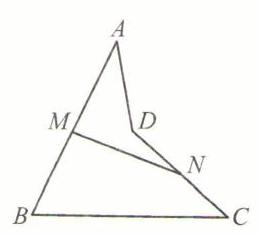
\includegraphics[width=0.2\textwidth]{bodyxb/src/bo_d20aucref24c73anc48g_136_1189_141_258_235_0.jpg}
    \end{center}
    \begin{jieda}
        取$BC$中点$P$，则$MP = \dfrac{1}{2}AC, PN = \dfrac{1}{2}BD$；$M,P,N$必不共线，否则与$A,B,C,D$共面矛盾，故有$MP+PN > MN$，故${AC} + {BD} > {2MN}$
    \end{jieda}
    \item 
    \begin{enumerate}
        \item 已知 ${AB},{BC},{CD}$ 为不在同一平面上的三条线段, ${AB},{BC},{CD}$ 的中点 $P,Q,R$ 满足 ${PQ} = 2,{QR} = \sqrt{5},{PR} = 3$ ,求 ${AC}$ 与 ${BD}$ 所成的角
        \begin{jieda}
            由三角形的中位线定理, ${PQ}//{AC}\text{ 、 }{QR}//{BD}$ . 又, $Q{P}^{2} + Q{R}^{2} = P{R}^{2} = 9$ ,由勾股定理的逆定理, $\therefore {QP} \bot  {QR}$ ,
            
            $\therefore {AC} \bot  {BD}$ ,即 ${AC}$ 与 ${BD}$ 所成的角为 ${90}^{ \circ  }$
        \end{jieda}
        \item 在空间四边形 ${ABCD}$ 中,已知 ${AD} = 1,{BC} = \sqrt{3}$ ,且 ${AD}\bot {BC}$ ,对角线 ${BD} = \dfrac{\sqrt{13}}{2},{AC} = \dfrac{\sqrt{3}}{2}$ ,求 ${AC}$ 和 ${BD}$ 所成的角
        \begin{jieda}
            取 ${AB},{AC},{AD},{CD}$ 的中点 $E,F,G,H$ . 由三角形的中位线定理,在 $\bigtriangleup  {EFH}$ 中, ${FE} = \dfrac{1}{2}{CB} = \dfrac{\sqrt{3}}{2},{FH} = \dfrac{1}{2}{AD} =$  $\dfrac{1}{2},{AD} \bot  {BC},\therefore {FH} \bot  {FE},\therefore {EH} = \sqrt{F{E}^{2} + F{H}^{2}} = 1$ ; 在 $\bigtriangleup {EGH}$ 中, ${GE} = \dfrac{1}{2}{DB} = \dfrac{\sqrt{13}}{4},{GH} = \dfrac{1}{2}{AC} =$  $\dfrac{\sqrt{3}}{4},G{E}^{2} + G{H}^{2} = E{H}^{2} = 1,\therefore {GE} \bot  {GH},\therefore {AC} \bot  {BD}$ ,即 ${AC}$ 与 ${BD}$ 所成的角为 ${90}^{ \circ  }$ 
        \end{jieda}
    \end{enumerate}
    \item 在正四面体 ${ABCD}$ 中,
    \threetu{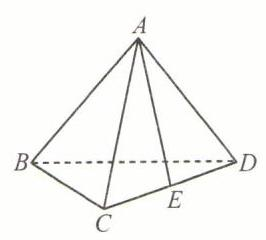
\includegraphics[width=0.6\textwidth]{bodyxb/src/bo_d20aucref24c73anc48g_136_277_839_266_240_0.jpg}}{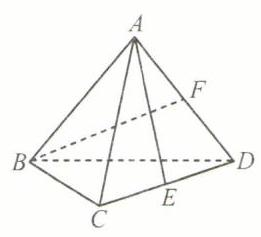
\includegraphics[width=0.6\textwidth]{bodyxb/src/bo_d20aucref24c73anc48g_136_652_841_261_237_0.jpg}}{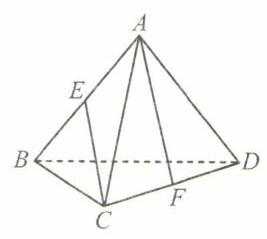
\includegraphics[width=0.6\textwidth]{bodyxb/src/bo_d20aucref24c73anc48g_136_1040_837_267_239_0.jpg}}
    \begin{enumerate}
        \item 若 $E$ 为棱 ${CD}$ 的中点 (如图),求 ${AE}$ 和 ${BC}$ 所成角的余弦值
        \begin{jieda}
            取$BD$中点$F$，则$\angle{AEF}$即为异面直线所成角（或其补角），根据余弦定理$cos\angle{AEF} = \dfrac{1+3-3}{2\sqrt{3}} = \dfrac{\sqrt{3}}{6}$
        \end{jieda}
        \item 已知 $E,F$ 分别是棱 ${CD},{AD}$ 的中点(如图),求 ${AE},{BF}$ 所成角的余弦值
        \begin{jieda}
            取$ED$中点$G$，则$\angle{BFG}$即为异面直线所成角（或其补角），根据余弦定理$cos\angle{BFG} = \dfrac{3+\dfrac{3}{4}-\dfrac{13}{4}}{3} = \dfrac{1}{6}$
        \end{jieda}
        \item 若 $E$ , $F$ 分别为棱 ${AB}$ , ${CD}$ 的中点(如图),求 ${AF}$ 与 ${CE}$ 所成角的正切值
        \begin{jieda}
            取$BF$中点$G$，则$\angle{CEG}$即为异面直线所成角（或其补角），根据余弦定理$cos\angle{BFG} = \dfrac{3+\dfrac{3}{4}-\dfrac{7}{4}}{3} = \dfrac{2}{3}$，故$tan\angle{BFG} = \dfrac{\sqrt{5}}{2}$
        \end{jieda}
    \end{enumerate}
    \item 已知直线 $a//$ 直线 $b,a$ 与平面 $\alpha$ 相交于点 $A$ ,求证: $b$ 与平面 $\alpha$ 必有公共点.
    \begin{jieda}
        直线$a$与直线$b$确定平面$\beta$，因为直线$a \cap \alpha = A$，所以$\alpha \cap \beta \neq \varnothing$，设其交线为$c$，即$c = \alpha \cap \beta$，有$a \cap c = A$

        假设$b$ 与平面 $\alpha$ 没有公共点，则$b \cap c = \varnothing$，因为$b,c \subset \beta$，所以$b // c$，因为$a // b$，所以$a // c$，与$a \cap c = A$矛盾

        因此 $b$ 与平面 $\alpha$ 必有公共点.
    \end{jieda}
    \item \begin{enumerate}
        \item 已知 $a,b$ 是异面直线,直线 $c$ 分别与 $a,b$ 相交于点 $P,Q$ ,直线 $d$ 分别与 $a,b$ 相交于点 $R,S$ ,求证: $c$ 和 $d$ 也是异面直线
        \begin{jieda}
            假设直线 $c,d$ 共面于平面 $\alpha$ ,则有 $P,Q,R,S \in  \alpha$ ,根据公理 1,直线 $a = {PR} \subset  \alpha$ ,直线 $b = {QS} \subset  \alpha$ ,这与直线 $a,b$ 是异面直线矛盾. 故直线 $c$ 和 $d$ 也是异面直线.
        \end{jieda}
        \item 过一点 $O$ 的三条直线 ${OA},{OB},{OC}$ 不共面,且 $D,E$ 在 ${OA}$ 上, $F$ 在 ${OB}$ 上, $G$ 在 ${OC}$ 上,求证: ${DF}$ 与 ${EG}$ 是异面直线
        \begin{jieda}
            假设直线 ${DF}$ , ${EG}$ 共面于平面 $\alpha$ ,则有 $D$ , $E$ , $F$ , $G \in  \alpha$ ,根据公理 1,直线 ${DE} = {OA} \subset  \alpha$ , $\therefore O \in$  ${DE} \subset  \alpha ,\therefore$ 直线 ${OA}$ (即 ${DE}$ ), ${OB}$ (即 ${OF}$ ), ${OC}$ (即 ${OG}$ ) $\subset  \alpha$ ,这与直线 ${OA},{OB},{OC}$ 不共面矛盾,故直线 ${DF}$ 与 ${EG}$ 是异面直线.
        \end{jieda}
        \item 已知平面 $\alpha$ 与平面 $\beta$ 相交于直线 ${CD}$ ,点 $A$ , $B$ 在 ${CD}$ 上,又直线 ${AE}$  $\subset  \alpha$ ,直线 ${BF} \subset  \beta$ (如图),求证: ${AE}$ 和 ${BF}$ 是异面直线.
        \begin{center}
        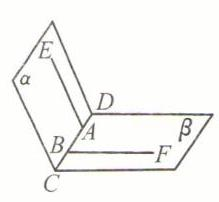
\includegraphics[width=0.2\textwidth]{bodyxb/src/bo_d20aucref24c73anc48g_136_1228_1215_219_202_0.jpg}
        \end{center}
        \begin{jieda}
            ${BF} \subset$ 平面 $\beta ,E \notin  \beta ,A \in  B$ ,且 ${BF}$ 不经过点 $A$ ,由异面直线判定定理 (平面外一点与平面内一点的连线,和平面内不经过该点的直线是异面直线),直线 ${AE}$ 与 ${BF}$ 是异面直线. 证毕.
        \end{jieda}
    \end{enumerate}

\end{enumerate}
\section*{三、直线与平面的位置关系}

\subsection*{(一) 直线和平面平行}

\subsubsection*{【典型题型和解题技巧】}

1. 直线和平面平行的证明.

证明直线和平面平行 (简称线面平行),通常有两种方法:

(1)利用线面平行的定义. 如果一条直线和一个平面没有公共点, 那么我们就说这条直线和这个平面平行.

若用数学符号表示,即直线 $l \cap$ 平面 $\alpha  = \varnothing  \Longrightarrow  l//\alpha$ .

利用线面平行的定义来证明线面平行, 在以后的学习中将会用到.

(2)利用线面平行的判定定理.

定理 如果平面外的一条直线和这个平面上的一条直线平行, 那么这条直线和这个平面平行.

我们把线面平行的判定定理概括为“若外内平行, 则线面平行”.

若用数学符号表示,即 $\left\{  \begin{array}{l} \text{ 直线 }l\text{ 不在平面 }\alpha \text{ 上, } \\  \text{ 直线 }m \subset  \text{ 平面 }\alpha , \\  l//m \end{array}\right\}   \Longrightarrow  l//\alpha$ .

\textbf{例 1} 已知有公共边 ${AB}$ 的两个全等的矩形 ${ABCD}$ 和 ${ABEF}$ 不在同一个平面上, $P,Q$ 分别是对角线 ${AE},{BD}$ 上的点,且 ${AP} = {DQ}$, 求证: ${PQ}//$ 平面 ${CBE}$ .

\begin{center}
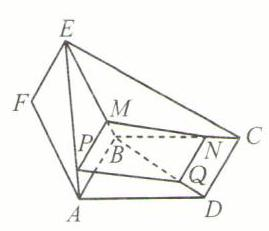
\includegraphics[width=0.2\textwidth]{bodyxb/src/bo_d20aucref24c73anc48g_137_1109_1274_269_231_0.jpg}
\end{center}

\textbf{分析} 

显然,直线 ${PQ}$ 在平面 ${CBE}$ 外,因此要证明 ${PQ}//$ 平面 ${CBE}$ , 只需要在平面 ${CBE}$ 内找一条直线,使 ${PQ}$ 平行于这条直线.

\textbf{证明} 

在平面 ${EAB}$ 上作 ${PM}//{AB}$ 交 ${BE}$ 于点 $M$ ,在平面 ${BCD}$ 上作 ${QN}//{AB}$ 交 ${BC}$ 于点 $N$ ,则 ${PM}//{QN}$ .由 $\dfrac{PM}{AB} = \dfrac{EP}{EA},\dfrac{QN}{CD} = \dfrac{BQ}{BD},{AP} = {DQ}$ ,得 ${EP} = {BQ}$ .又 ${AB} = {CD},{EA} = {BD}$ ,故 ${PM} = {QN}$ ,于是四边形 ${PMNQ}$ 是平行四边形,$\therefore {PQ}//{MN}$ .

综上所述, ${PQ}$ 不在平面 ${CBE}$ 上, ${MN} \subset$ 平面 ${CBE},{PQ}//{MN}$，$\therefore {PQ}//$ 平面 ${CBE}$ .

注意 我们的“口诀”中特别强调了“上”(平面上的直线),“外”(平面外的直线)两个字. 在运用线面平行的判定定理时,一定要写明哪条直线在平面外,哪条直线在平面上.

2. 直线和平面平行的性质.

直线和平面平行的性质有:

(1)利用线面平行的定义, 如果一条直线和一个平面平行, 那么这条直线和这个平面没有公共点, 简记为

$
\text{ 直线 }l//\text{ 平面 }\alpha  \Longrightarrow  l \cap  \alpha  = \varnothing \text{ . }
$

(2)线面平行的性质定理.

定理 如果一条直线和一个平面平行, 经过这条直线的平面和这个平面相交, 那么这条直线和交线平行.

我们把线面平行的性质定理概括为 “若线面平行,则线线平行”,这里特别重要的是 “作辅助平面”这个中间程序, 简记为

$
\left. \begin{array}{l} \text{ 直线 }l//\text{ 平面 }\alpha , \\  \text{ 直线 }l \subset  \text{ 平面 }\beta , \\  \alpha  \cap  \beta  = \text{ 直线 }m, \end{array}\right\}   \Longrightarrow  l//m\text{ . }
$

\textbf{例 2} 已知: 直线 $l//$ 平面 $\alpha$ ,直线 $m//l,m$ 不在平面 $\alpha$ 上,求证: $m//\alpha$ .

\textbf{错证} 

如图(1),在平面 $\alpha$ 内作直线 $n//l,\because m//l,\therefore m//n$ ,而 $m$ 不在平面 $\alpha$ 上, $n \subset$  $\alpha ,\therefore m//\alpha$ .

\textbf{分析} 

线面平行的性质定理是: “如果一条直线和一个平面平行, 经过这条直线的平面和这个平面相交, 那么这条直线就和交线平行".

定理中沟通条件“线面平行”和结论“线线平行”的渠道是“经过这条直线的平面和这个平面相交”,而上述的证明中并没有出现这种平面,只是随心所欲地在 $\alpha$ 内作直线 $n//l$ (尽管这种直线客观存在),错误正在于此(初次接触立体几何,这种错误最容易犯).

\begin{center}
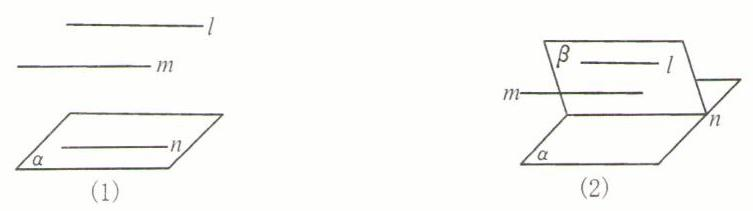
\includegraphics[width=0.6\textwidth]{bodyxb/src/bo_d20aucref24c73anc48g_138_420_1343_753_211_0.jpg}
\end{center}


\textbf{证明} 

如图(2),过 $l$ 作平面 $\beta$ ,使 $\beta  \cap  \alpha  = n$ .

$\because l//\alpha ,\therefore l//n$ . 又 $\because m//l,\therefore m//n$ . 又 $\because m$ 不在平面 $\alpha$ 上, $n \subset  \alpha ,\therefore m//\alpha$ .

注意 正确运用线面平行性质定理的关键是:过已知直线作一个辅助平面.

\subsubsection*{【训练题】}

\begin{center}  \textbf{(A)} \end{center}
\begin{enumerate}
    \item 已知直线 $l//$ 平面 $\alpha$ ,直线 $a \subset  \alpha$ ,则 $l$ 与 $a$ 的位置关系必定是\dotfill{(\kh{D})}
    \xx{$l//a$}{$l$ 与 $a$ 异面}{$l$ 与 $a$ 相交}{$l$ 与 $a$ 无公共点}
    \begin{jieda}
        由线面平行的定义, $l \cap  \alpha  = \varnothing$ ,而 $a \subset  \alpha ,\therefore l \cap  a = \varnothing$ ,选项 $D$ 正确,选项 $C$ 错误. 在正方体 ${ABCD} -$  ${A}^{\prime }{B}^{\prime }{C}^{\prime }{D}^{\prime }$ 中,取 $l = {B}^{\prime }{C}^{\prime },\alpha  = {ABCD}$ ,若 $a = {BC}$ ,则 $l//a$ ; 若 $a = {AB}$ ,则 $l$ 与 $a$ 异面,故选项 $A,B$ 均错误.
    \end{jieda}
    \item $a,b$ 是两条直线, $\alpha$ 是平面. 给出以下四个命题:
    \begin{dingautolist}{172}
        \item 若 $a//\alpha ,b//\alpha$ ,则 $a//b$
        \item 若 $a//b,a//\alpha$ , 则 $b//\alpha$
        \item 若 $a//\alpha$ ,则 $a//\alpha$ 上所有直线
        \item 若 $a//\alpha$ 上无数条直线,则 $a//\alpha$
    \end{dingautolist}
    其中正确的个数是\dotfill{(\kh{A})}
    \xx{0}{1}{2}{3}
    \begin{jieda}
        \begin{dingautolist}{172}
            \item 三种位置关系均有可能
            \item $b$可能在$\alpha$内
            \item 存在异面的直线
            \item $a$可能在$\alpha$内
        \end{dingautolist}
    \end{jieda}
    \item 若直线 $a$ 平行于平面 $\alpha$ 上的直线 $b$ ,则 $a$ 和 $\alpha$ 的位置关系是\dotfill{(\kh{C})}
    \xx{$a//\alpha$}{$a \subset  \alpha$}{$a//\alpha$ 或 $a \subset  \alpha$}{$a//\alpha$ 或 $a$ 与 $\alpha$ 相交}
    \begin{jieda}
        若直线 $a$ 不在平面 $\alpha$ 上,则 $a//\alpha$ ; 若直线 $a$ 在平面 $\alpha$ 上,则 $a \subset  \alpha$
    \end{jieda}
    \item 已知不重合的直线 $a,b,c$ 及平面 $\alpha$ ,则下列条件能使 $a//b$ 成立的是 \dotfill{(\kh{C})}
    \xx{$a//\alpha$ 且 $b//\alpha$}{$a\bot c$ 且 $b\bot c$}{$a//c$ 且 $b//c$}{$a//\alpha$ 且 $a\bot c$}
    \begin{jieda}
        根据公理 4,选项 C 能推出 $a//b$ .
    \end{jieda}
    \item 给出四个命题:
    \begin{dingautolist}{172}
        \item ${AB}$ 为平面 $\alpha$ 外的线段,若点 $A,B$ 到平面 $\alpha$ 的距离相等,则 ${AB}//\alpha$
        \item 若一个角的两边分别平行于另一个角的两边,则这两个角相等
        \item 若直线 $a//$ 直线 $b$ ,则 $a$ 平行于过 $b$ 的所有平面
        \item 若直线 $a//$ 平面 $\alpha$ ,直线 $b//$ 平面 $\alpha$ ,则 $a//b$
    \end{dingautolist}
    其中正确的个数是\dotfill{(\kh{A})}
    \xx{0}{1}{2}{3}
    \begin{jieda}
        \begin{dingautolist}{172}
            \item 注意 $A,B$ 两点分别在平面 $\alpha$ 两侧的可能性
            \item 注意这两个角互补的可能性
            \item 直线 $a,b$ 本身可以确定一个平面,此时 $a$ 在该平面内
            \item 三种位置关系都有可能
        \end{dingautolist}
    \end{jieda}
    \item \begin{enumerate}
        \item 若直线 $l$ 与平面 $\alpha$ 平行,则在平面 $\alpha$ 内与 $l$ 平行的直线有\blkda{无数}条
        \begin{jieda}
            过直线 $l$ 可以作无数个互不重合的平面,它们与平面 $\alpha$ 的交线 (如有) 有无数条,也互不重合,且都与直线 $l$ 平行；或者,过直线 $l$ 作 1 个平面与平面 $\alpha$ 相交,交线记为 ${l}^{\prime }$ ,而在平面 $\alpha$ 内有无数条直线与 ${l}^{\prime }$ 平行,根据公理 4, 它们都与直线 $l$ 平行.
        \end{jieda}
        \item 若 $P$ 是平面 $\alpha$ 外一点,则过 $P$ 作 $\alpha$ 的平行线有\blkda{无数}条
        \begin{jieda}
            在平面 $\alpha$ 内先取一点 ${P}^{\prime }$ ,再任取一点 ${Q}^{\prime }$ 异于点 ${P}^{\prime }$ ,则过 ${P}^{\prime },{Q}^{\prime },P$ 三点可确定一个平面,记为平面 $\beta$ . 在平面 $\beta$ 内,过点 $P$ 可以作一条直线 ${PQ}//{P}^{\prime }{Q}^{\prime }$ ,此时 ${PQ}//$ 平面 $\alpha$ . 当射线 ${P}^{\prime }{Q}^{\prime }$ 的方向不断变化时, ${PQ}$ 的方向也不断变化,便能得到无数条过点 $P$ 与平面 $\alpha$ 平行的直线. 或者,在学过两个平面平行的知识后,结合立体解析几何,可知: 过点 $P$ 可作唯一平面 $\beta$ 与平面 $\alpha$ 平行 (这两个平面的法向量相同),而平面 $\beta$ 中任意过点 $P$ 的直线都与平面 $\alpha$ 平行, 这样的直线有无数条.
        \end{jieda}
        \item 已知两直线 $a//b,a,b \subset$ 平面 $\alpha$ ,直线 $c$ 与 $a$ 异面, $c \cap  b = \varnothing$ ,则 $c$ 与 $\alpha$ 的位置关系是\blkda[2]{平行或相交}
        \begin{jieda}
            直线和平面的关系有 3 种:平行、相交或直线在平面上. 由于直线 $c$ 与 $a$ 异面,故直线不可能在平面上. 在正方体 ${ABCD} - {A}^{\prime }{B}^{\prime }{C}^{\prime }{D}^{\prime }$ 中,取 $a = {AB},b = {CD},\alpha  = {ABCD}$ ,若 $c = {B}^{\prime }{C}^{\prime }$ ,则 $c//\alpha$ ; 取 ${A}^{\prime }{D}^{\prime }$ 和 ${BC}$ 中点 $F,G$ , 若 $c = {FG}$ ,则 $c$ 与 $\alpha$ 相交.
        \end{jieda}
    \end{enumerate}
    
    \item 已知 ${AB}$ 是平面 $\alpha$ 外的一条直线,过 ${AB}$ 的平面 $\beta$ ,平面 $\gamma$ 与 $\alpha$ 分别交于直线 $a,b$ . 若 $a//b$ (如图),求证: ${AB}//\alpha$ .
    \begin{center}
    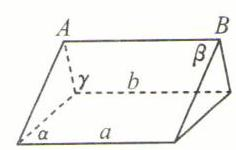
\includegraphics[width=0.2\textwidth]{bodyxb/src/bo_d20aucref24c73anc48g_139_1138_1046_236_150_0.jpg}
    \end{center}
    \begin{jieda}
        假设$AB$不平行于$\alpha$，则可设$AB \cap \alpha = C$，根据公理3可知$C \in a, C \in b$，故$a \cap b = c$，与$a // b$矛盾，故${AB}//\alpha$
    \end{jieda}
    
    \item \begin{enumerate}
        \item 在正方体 ${ABCD} - {A}^{\prime }{B}^{\prime }{C}^{\prime }{D}^{\prime }$ 中, $E$ 是 $D{D}^{\prime }$ 的中点 (如图),求证: ${B}^{\prime }D//$ 平面 ${A}^{\prime }{C}^{\prime }E$
        \begin{center}
        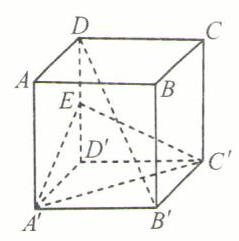
\includegraphics[width=0.2\textwidth]{bodyxb/src/bo_d20aucref24c73anc48g_139_366_1352_239_241_0.jpg}
        \end{center}
        \begin{jieda}
            证明：连接 ${B}^{\prime }{D}^{\prime }$ 与 ${A}^{\prime }{C}^{\prime }$ 相交于点 $O$ ,连接 ${OE}$ . 在 $\bigtriangleup {B}^{\prime }{D}^{\prime }D$ 中,易知 ${OE}$ 是 ${B}^{\prime }D$ 边对应的中位线,故 ${OE}//{B}^{\prime }D$ . 又 ${OE} \subset$ 平面 ${A}^{\prime }{C}^{\prime }E,{B}^{\prime }D$ 在平面 ${A}^{\prime }{C}^{\prime }E$ 外,故 ${B}^{\prime }D//$ 平面 ${A}^{\prime }{C}^{\prime }E$ ,证毕.
        \end{jieda}
        \item 已知 ${AB},{BC},{CD}$ 是不在同一平面上的三条线段(如图),求证:经过 ${AB},{BC},{CD}$ 的中点 $E,F,G$ 的平面平行于 ${AC}$ 和 ${BD}$
        \begin{center}
        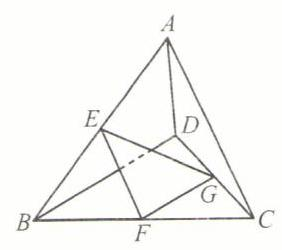
\includegraphics[width=0.2\textwidth]{bodyxb/src/bo_d20aucref24c73anc48g_139_865_1335_282_250_0.jpg}
        \end{center}
        \begin{jieda}
            证明:在 $\bigtriangleup  {ABC}$ 中,易知 ${EF}$ 是 ${AC}$ 边对应的中位线,故 ${EF}//{AC}$ . 又 ${EF} \subset$ 平面 ${EFG}$ , ${AC}$ 在平面 ${EFG}$ 外,故 ${AC}//$ 平面 ${EFG}$ ; 在 $\bigtriangleup {BCD}$ 中,易知 ${FG}$ 是 ${BD}$ 边对应的中位线,故 ${FG}//{BD}$ . 又 ${FG} \subset$ 平面 ${EFG},{BD}$ 在平面 ${EFG}$ 外,故 ${BD}$ //平面 ${EFG}$ ,证毕.
        \end{jieda}
        \item 已知 $P$ 为平行四边形 ${ABCD}$ 所在平面外一点, $M$ 为 ${PB}$ 的中点 (如图),求证: ${PD}//$ 平面 ${MAC}$
        \begin{center}
        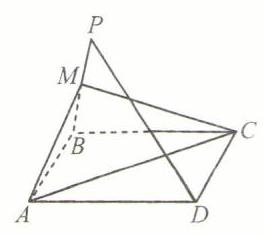
\includegraphics[width=0.2\textwidth]{bodyxb/src/bo_d20aucref24c73anc48g_139_372_1859_264_234_0.jpg}
        \end{center}
        \begin{jieda}
            证明:连接 ${BD}$ 与 ${AC}$ 相交于点 $O$ ,连接 ${OM}$ . 在 $\bigtriangleup  {BDP}$ 中,易知 ${OM}$ 是 ${PD}$ 边对应的中位线,故 ${OM}//{PD}$ . 又 ${OM} \subset$ 平面 ${MAC},{PD}$ 在平面 ${MAC}$ 外,故 ${PD}//$ 平面 ${MAC}$ ,证毕.
        \end{jieda}
        \item 已知 $E,F$ 分别为正方体 ${ABCD} - {A}_{1}{B}_{1}{C}_{1}{D}_{1}$ 的棱 ${BC},{C}_{1}{D}_{1}$ 的中点 (如图),求证: ${EF}//$ 平面 $B{B}_{1}{D}_{1}D$ .
        \begin{center}
        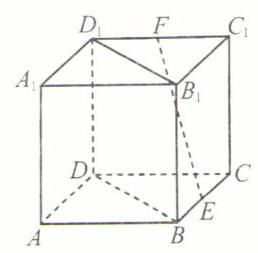
\includegraphics[width=0.2\textwidth]{bodyxb/src/bo_d20aucref24c73anc48g_139_893_1832_258_253_0.jpg}
        \end{center}
        \begin{jieda}
            连接 ${A}_{1}{C}_{1}$ 与 ${B}_{1}{D}_{1}$ 相交于点 $O$ ,连接 ${OF}$ , ${OB}$ ,关键是证明 ${FE}//{OB}$ . 在 $\bigtriangleup {B}_{1}{C}_{1}{D}_{1}$ 中,易知 ${OF}$ 是 ${B}_{1}{C}_{1}$ 边对应的中位线,故 ${OF}//{B}_{1}{C}_{1}$ 且 ${OF} = \dfrac{1}{2}{B}_{1}{C}_{1}$ . 又 ${BE}//{B}_{1}{C}_{1}$ 且 ${BE} = \dfrac{1}{2}{BC} = \dfrac{1}{2}{B}_{1}{C}_{1} = {OF}$ ,结合公理 4,可知 ${OF}\bot {BE}$ , $\therefore$ 四边形 ${OBEF}$ 是平行四边形. $\therefore {FE}//{OB}$ ,又 ${OB} \subset$ 平面 $B{B}_{1}{D}_{1}D,{FE}$ 在平面 $B{B}_{1}{D}_{1}D$ 外,故 ${FE}//$ 平面 $B{B}_{1}{D}_{1}D$ ,证毕.
        \end{jieda}
    \end{enumerate}
    \item  在正方体 ${ABCD} - {A}_{1}{B}_{1}{C}_{1}{D}_{1}$ 中画出:
    \begin{enumerate}
        \item 与 ${AC}$ 平行且仅过正方体三个顶点的截面
        \item 过 ${A}_{1}{C}_{1}$ 且与 ${B}_{1}D$ 平行的截面
    \end{enumerate}
    \begin{jieda}
        \begin{enumerate}
            \item 截面 ${A}_{1}{C}_{1}B$ 和截面 ${A}_{1}{C}_{1}D$ ,均符合题意
            \item 取 $D{D}_{1}$ 的中点 $M$ ,平面 $M{A}_{1}{C}_{1}$ 即为所求
        \end{enumerate}
    \end{jieda}

\end{enumerate}

\begin{center}  \textbf{(B)} \end{center}
\begin{enumerate}
    \item 如果 $a,b$ 是异面直线,给出以下三个结论:
    \begin{dingautolist}{172}
        \item 过空间内任何一点可以作一个和 $a,b$ 都平行的平面
        \item 过直线 $a$ 有且只有一个平面和 $b$ 平行
        \item 过空间内任何一点可以作一条直线和 $a,b$ 都相交
    \end{dingautolist}
    其中错误的个数是 \dotfill{(\kh{C})}
    \xx{0}{1}{2}{3}
    \begin{jieda}
        \begin{dingautolist}{172}
            \item 一个特殊的反例是点 $M$ 在直线 $a$ 或 $b$ 上，一般的反例是\ding{173}的平面内
            \item 存在性及具体作法: 在直线 $b$ 上任取一点 $P$ ,在直线 $a$ 上任取两点 $Q\text{ 、 }R$ ,在平面 ${PQR}$ 中 (即点 $P$ 和直线 $a$ 确定的平面),过点 $P$ 作直线 $a$ 的平行线 ${a}^{\prime }$ (可由尺规作图,构造平行四边形得到). 此时,相交直线 ${a}^{\prime }$ 和 $b$ 确定的平面即为平面 $\alpha$
            
            唯一性证明如下: (反证法) 假设所求平面不唯一,记平面 $\alpha ,\beta$ 均满足题意. 在直线 $a$ 上任取一点 $M$ ,则过点 $M$ 和直线 $b$ 可以确定一个平面 $\gamma .\because M \in  \gamma$ 且 $M \in  \alpha ,M \in  \beta$ ,根据公理 $3,\gamma$ 与 $\alpha$ 和 $\beta$ 都相交,交线记为 ${l}_{\alpha }$ 和 ${l}_{\beta }$ . 由线面平行的性质定理, ${l}_{\alpha }//b,{l}_{\beta }//b$ ,根据公理 $4,{l}_{\alpha }//{l}_{\beta }$ ,这与 ${l}_{\alpha } \cap  {l}_{\beta } = M$ 矛盾,故所求平面是唯一的,证毕.
            \item 反例：不在直线上，但在\ding{173}的平面内
        \end{dingautolist}
    \end{jieda}
    \item 如果点 $M$ 是两条异面直线 $a,b$ 外的一点,则过点 $M$ 且与 $a,b$ 都平行的平面 \dotfill{(\kh{C})}
    \xx{只有一个}{恰有两个}{或者没有, 或者只有一个}{有无数个}
    \item 已知 $A,B,C,D$ 是空间不共面的四点,它们到平面 $\alpha$ 的距离相等,则满足条件的平面 $\alpha$ 的个数是\dotfill{(\kh{C})}
    \xx{3}{4}{7}{8}
    \begin{jieda}
        按平面 $\alpha$ 两侧点的数量讨论: 
        \begin{dingautolist}{172}
            \item 若 4 点都在平面 $\alpha$ 的同侧,则四点共面,与题干矛盾
            \item 若只有 3 点在平面 $\alpha$ 的同侧有 4 种可能,现以同侧 3 点为点 $A,B,C$ 为例,此时平面 $\alpha //$ 平面 ${ABC}$ ,再加上 “距离相等” 的约束,故所求平面是唯一的,具体而言: 取线段 ${DA},{DB},{DC}$ 的中点,连接所得的平面即为所求
            \item 若只有 2 点在平面 $\alpha$ 的同侧,有 3 种可能,现以点 $A,B$ 和点 $C,D$ 分属平面 $\alpha$ 的两侧为例,此时 ${AB}//$ 平面 $\alpha ,{CD}//$ 平面 $\alpha ,{AB}$ 与 ${CD}$ 的公垂线段上平面 $\alpha$ ,“距离相等”的约束要求平面 $\alpha$ 经过 ${AB}$ 与 ${CD}$ 的公垂线段的中点
        \end{dingautolist}
        综上,满足条件的平面个数为 7 个.
    \end{jieda}
    \item 已知异面直线 ${AB},{CD}$ 都平行于平面 $\alpha$ ,且 ${AB},{CD}$ 在 $\alpha$ 的两侧,若 ${AC},{BD}$ 与 $\alpha$ 分别交于 $M,N$ 两点 (如图),求证: $\dfrac{AM}{MC} = \dfrac{BN}{ND}$ .
    
    \begin{center}
    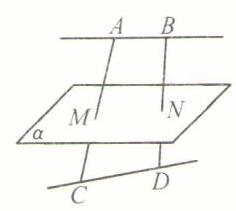
\includegraphics[width=0.2\textwidth]{bodyxb/src/bo_d20aucref24c73anc48g_140_1201_1111_236_211_0.jpg}
    \end{center}
    \begin{jieda}
        连接 ${AD}$ 交 $\alpha$ 于 $Q$ ,则可证 ${CD}//{MQ}$ ,于是 $\dfrac{AM}{MC} = \dfrac{AQ}{QD}$ . 同理可证 $\dfrac{AQ}{QD} = \dfrac{BN}{ND}$，故$\dfrac{AM}{MC} = \dfrac{NB}{ND}$ 
    \end{jieda}
    \item 已知 $P,Q$ 是单位正方体 ${ABCD} - {A}_{1}{B}_{1}{C}_{1}{D}_{1}$ 的面 $A{A}_{1}{D}_{1}D$ ,面 ${A}_{1}{B}_{1}{C}_{1}{D}_{1}$ 的中心 (如图).
    \begin{center}
    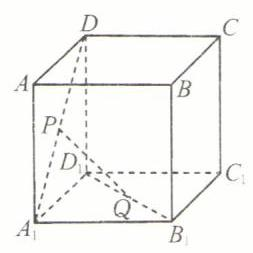
\includegraphics[width=0.2\textwidth]{bodyxb/src/bo_d20aucref24c73anc48g_140_392_1501_253_253_0.jpg}
    \end{center}
    \begin{enumerate}
        \item 求线段 ${PQ}$ 的长
        \item 求证: ${PQ}//$ 平面 $A{A}_{1}{B}_{1}B$ 
    \end{enumerate}
    \begin{jieda}
        \begin{enumerate}
            \item 连接 ${A}_{1}{C}_{1}$ ,与 ${B}_{1}{D}_{1}$ 的交点即点 $Q$ . 在 $\bigtriangleup D{A}_{1}{C}_{1}$ 中, ${PQ}$ 是 $D{C}_{1}$ 边上的中位线,故 ${PQ}//D{C}_{1}$ 且 ${PQ} =$  $\dfrac{1}{2}D{C}_{1} = \dfrac{\sqrt{2}}{2}$ . 
            \item 从上一问可知${PQ}//D{C}_{1}$ ,而 $D{C}_{1}//A{B}_{1}$ ,故 ${PQ}//A{B}_{1}$ ,进而 ${PQ}//$ 平面 $A{A}_{1}{B}_{1}B$ ,证毕.
        \end{enumerate}
    \end{jieda}
    \item 用平行于四面体 ${ABCD}$ 的一组对棱 ${AB}$ , ${CD}$ 的平面截此四面体(如图).
    \begin{center}
    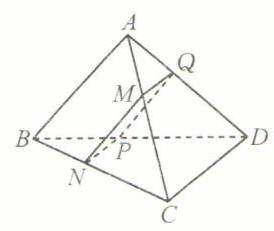
\includegraphics[width=0.2\textwidth]{bodyxb/src/bo_d20aucref24c73anc48g_140_902_1520_274_231_0.jpg}
    \end{center}
    \begin{enumerate}
        \item 求证:所得截面 ${MNPQ}$ 是平行四边形
        \item 如果 ${AB} = {CD} = a$ ,求证:四边形 ${MNPQ}$ 的周长为定值
        \item 如果 ${AB} = a,{CD} = b,{AB},{CD}$ 所成角为 $\theta$ ,求四边形 ${MNPQ}$ 面积的最大值,并确定此时点 $M$ 的位置
    \end{enumerate}
    \begin{jieda}
        \begin{enumerate}
            \item 由线面平行的性质定理可知${AB}//{MN},{AB}//{PQ}$ ,再由公理 $4,{MN}//{PQ}$ ,故 ${MN}$ 和 ${PQ}$ 确定一个平面,四边形 ${MNPQ}$ 是平面图形. 同理, ${MQ}//{NP}\left( {//{CD}}\right)$ 
            
            $\therefore {MNPQ}$ 是平行四边形,证毕.
            \item 在 $\bigtriangleup {ABC}$ 中, ${AB}//{MN}$ ,故 $\dfrac{MN}{AB} = \dfrac{CM}{CA}$ ；同理,在 $\bigtriangleup {ACD}$ 中, $\dfrac{MQ}{CD} = \dfrac{MA}{CA}$ . $\therefore$ 平行四边形 ${MNPQ}$ 的周长为 $2\left( {{MN} + {MQ}}\right)  = 2 \cdot  \left( {\dfrac{CM}{CA} + \dfrac{MA}{CA}}\right)  \cdot  a = {2a}$ ,为定值,证毕.
            
            \item 记 ${AC} = c,{CM} = x$，则 $S = MN \cdot MQ \cdot sin\angle{MNP}$
            
            $\dfrac{MN}{a} = \dfrac{x}{c}, \dfrac{MQ}{b} = \dfrac{c-x}{c}$，$\angle{MNP} = \theta$，故$S = \dfrac{ab[x(c-x)]}{c^2}sin\theta$
            
            当 $M$ 为 ${AC}$ 中点时, ${S}_{\max } = \dfrac{1}{4}{ab}\sin \theta$ .
        \end{enumerate}
    \end{jieda}
    \item 已知直线 $l//$ 平面 $\alpha ,l//$ 平面 $\beta$ ,且 $\alpha  \cap  \beta  = m$ (如图),求证: $l//m$ .

    \begin{center}
    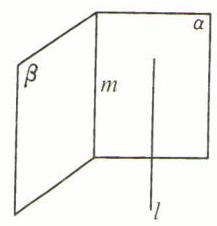
\includegraphics[width=0.2\textwidth]{bodyxb/src/bo_d20aucref24c73anc48g_141_342_212_217_226_0.jpg}
    \end{center}
    \begin{jieda}
        过 $l$ 作平面 $\gamma$ ,使 $\gamma  \cap  \alpha  = a$ ,过 $l$ 作平面 $\delta$ ,使 $\delta  \cap  \beta  = b$ ,则 $l//a,l//b$ ,于是 $a//b$ ,故 $a//\beta$ ,由此得 $a//m,\therefore l//m$
    \end{jieda}
    \item 已知直线 $l//$ 平面 $\alpha$ ,直线 $m//l$ ,且点 $A \in  \alpha ,A \in  m$ (如图),求证: $m \subset  \alpha$ .
    \begin{center}
    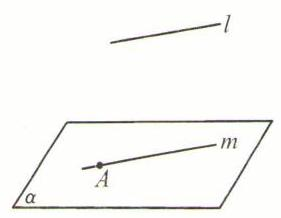
\includegraphics[width=0.2\textwidth]{bodyxb/src/bo_d20aucref24c73anc48g_141_822_219_281_218_0.jpg}
    \end{center}
    \begin{jieda}
        设$l$和$m$构成平面$\beta$，设$\beta \cap \alpha = n$，因为$A \in \alpha, A \in \beta$，所以$A \in n$

        假设$m \neq n$，则$l // \alpha \Longrightarrow l // n \Longrightarrow m // n$，与$A \in m, a \in n$矛盾

        故$m \subset \alpha$
    \end{jieda}
\end{enumerate}

\subsection*{(二) 直线和平面垂直}

\subsubsection*{【典型题型和解题技巧】}

1. 直线和平面垂直的证明.

(1)利用线面垂直的定义.

\textbf{定义} 如果一条直线和一个平面上的任何一条直线都垂直, 我们说这条直线和这个平面互相垂直.

因此, 要证明一条直线和一个平面垂直, 只需证明这条直线和这个平面上任意一条直线垂直.

\textbf{例 1} 已知直线 $a//$ 直线 $b,a\bot$ 平面 $\alpha$，求证: $b\bot \alpha$ .

\begin{center}
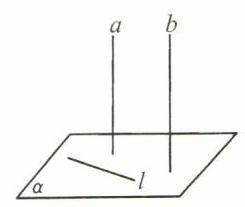
\includegraphics[width=0.2\textwidth]{bodyxb/src/bo_d20aucref24c73anc48g_141_1139_1135_245_207_0.jpg}
\end{center}

\textbf{证明} 

设 $l$ 是 $\alpha$ 内任意一条直线. ” 因为$a \bot \alpha$ , $l \subset  \alpha$，所以$a \bot  l$，而 $b//a,\therefore b \bot  l,b \bot  \alpha$ .

(2)利用线面垂直的判定定理.

\textbf{定理} 如果一条直线和一个平面上的两条相交直线都垂直, 那么这条直线垂直于这个平面.

\textbf{例 2} 已知 ${PA} \bot   \odot  O$ 所在的平面, ${AB}$ 是 $\odot  O$ 的直径, $C$ 是 $\odot  O$ 上任意一点,过点 $A$ 作 ${AE} \bot  {PC}$ 于点 $E$，求证: ${AE} \bot$ 平面 ${PBC}$ .

\begin{center}
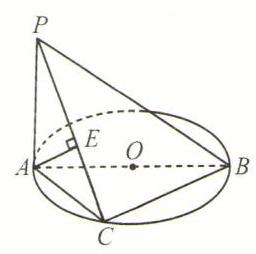
\includegraphics[width=0.2\textwidth]{bodyxb/src/bo_d20aucref24c73anc48g_141_1131_1598_256_254_0.jpg}
\end{center}

\textbf{证明} 

$\because {PA} \bot$ 平面 ${ABC},\therefore {PA} \bot  {BC}$，又 $\because {AB}$ 是 $\odot  O$ 的直径, $\therefore {BC} \bot  {AC}$，而 ${PA} \cap  {AC} = A,\therefore {BC} \bot$ 平面 ${PAC}$ .

又 $\because {AE} \subset$ 平面 ${PAC},\therefore {BC} \bot  {AE}$，$\because {PC} \bot  {AE}$ ,且 ${PC} \cap  {BC} = C,\therefore {AE} \bot$ 平面 ${PBC}$ .


\textbf{例 3} 已知 ${PA} \bot$ 平面 $\alpha ,{PB} \bot$ 平面 $\beta ,A,B$ 为相应的垂足,且 $l$ 为平面 $\alpha$ 与平面 $\beta$ 的交线. 求证: $l \bot$ 平面 ${PAB}$ .

\textbf{证明} 

因为 ${PA} \bot$ 平面 $\alpha$ ,且 $l$ 在平面 $\alpha$ 上,所以 ${PA} \bot  l$ ,同理 ${PB} \bot  l$ . 因为 ${PA} \cap  {PB} = P$ , 所以 $l \bot$ 平面 ${PAB}$ .

(3)利用线面垂直判定定理的推论.

\textbf{推论} 如果两条平行直线中的一条垂直于一个平面, 那么另一条也垂直于这个平面. 

简记 $\left. \begin{array}{l} \text{ 直线 }a//\text{ 直线 }b, \\  \text{ 直线 }a \bot  \text{ 平面 }\alpha , \end{array}\right\}   \Longrightarrow  b \bot  \alpha$ .

2. 线面垂直的性质.

(1)利用线面垂直的定义,如果一条直线垂直于一个平面,那么这条直线就垂直于这个平面上的任意一条直线.

(2)线面垂直的性质定理.

\textbf{定理} 如果两条直线同垂直于一个平面,那么这两条直线平行.

\subsubsection*{【训练题】}

\begin{center}  \textbf{(A)} \end{center}
\begin{enumerate}
    \item 下列命题正确的是\dotfill{(\kh{D})}
    \xx{如果两条直线都与第三条直线垂直, 那么这两条直线互相平行}{如果两条直线都与同一平面平行, 那么这两条直线互相平行}{如果一条直线与一个平面上的无数条直线垂直, 那么这条直线与这个平面垂直}{如果两条平行直线中的一条垂直于一个平面, 那么另一条也垂直于这个平面}
    \begin{jieda}
        选项 (D) 即线面垂直判定定理的推论. 借助正方体 ${ABCD} - {A}^{\prime }{B}^{\prime }{C}^{\prime }{D}^{\prime }$ ,对其余选项分析如下:选项 (A) ,也可以相交或异面,如:两直线为 ${AB}$ , ${AD}$ (或 ${AB}$ , ${A}^{\prime }{D}^{\prime }$ ),第三条直线为 $A{A}^{\prime }$ ,则两直线相交(异面)；选项(B),也可以相交或异面,如: 取两直线为 ${AB}$ , ${AD}$ ,平面为 ${A}^{\prime }{B}^{\prime }{C}^{\prime }{D}^{\prime }$ ,则两直线相交; 选项 (C),也可以相交 (但不垂直)、平行或在平面内,需注意“无数条直线”和“任意直线”的区别.
    \end{jieda}
    \item 已知三条直线 $a,b,l$ 及平面 $\alpha ,\beta$ ,则下列命题正确的是 \dotfill{(\kh{B})}
    \xx{若 $b \subset  \alpha ,a//b$ ,则 $a//\alpha$}{若 $a \bot  \alpha ,b \bot  \alpha$ ,则 $a//b$}{若 $a//\alpha ,\alpha  \cap  \beta  = b$ ,则 $a//b$}{若 $a \subset  \alpha ,b \subset  \alpha ,l \bot  a,l \bot  b$ ,则 $l \bot  \alpha$}
    \begin{jieda}
        选项 (A) 需注意直线 $a$ 在平面 $\alpha$ 内的可能性. 错误；选项 (B) 即线面垂直的性质定理,正确；选项 (C) 中,平面 $\beta$ 不一定通过直线 $a$ ,故直线 $b$ 事实上是任意的,因此直线 $a$ , $b$ 也可能异面,错误；选项 (D),需注意 $a//b$ 的可能性,此时 $l$ 与 $\alpha$ 可以相交 (但不垂直)、平行或在平面 $\alpha$ 内,错误.
    \end{jieda}
    \item 给出以下四个命题:\ding{172}若直线 $l$ 不在平面平面 $\alpha$ 上,则 $l$ 不可能与 $\alpha$ 内无数条直线相交；\ding{173} 若直线 $l$ 与平面 $\alpha$ 不平行,则 $l$ 与 $\alpha$ 内任一直线都不平行；\ding{174}若直线 $l$ 与平面 $\alpha$ 不垂直,则 $l$ 不可能垂直于 $\alpha$ 内无数条直线；\ding{175}若平面 $\alpha$ 内有一条直线和直线 $l$ 异面,则 $l$ 不在平面 $\alpha$ 上. 其中正确的个数是\dotfill{(\kh{B})}
    \xx{0}{1}{2}{3}
    \begin{jieda}
        对于\ding{172},设直线 $l$ 与平面 $\alpha$ 相交于 $O$ 点,则平面 $\alpha$ 内过 $O$ 点的任意直线都满足要求,错误；对于\ding{173},若直线 $l$ 在平面 $\alpha$ 内,则平面 $\alpha$ 内可以作无数条直线与 $l$ 平行,错误；对于\ding{174},不论直线 $l$ 与平面 $\alpha$ 相交(但不垂直)、平行或在平面 $\alpha$ 内, 都能在 $\alpha$ 内找到无数条直线与直线 $l$ 垂直,例如在正方体 ${ABCD} - {A}^{\prime }{B}^{\prime }{C}^{\prime }{D}^{\prime }$ 中,取 $\alpha  =$ 平面 ${ABCD},l = A{D}^{\prime }$ (或 ${A}^{\prime }{D}^{\prime }$ 或 ${AD}$ ),则 $\alpha$ 内任意与 ${AB}$ 平行的直线均符合要求,错误; 对于\ding{175},本命题的逆否命题是: 若 $l \subset  \alpha$ ,则平面 $\alpha$ 内的所有直线都与直线 $l$ 共面,这是真命题,正确. 综上,正确的个数是 1 个. 注: 对于\ding{175},也可使用反证法. 另外,“平面 $\alpha$ 内有一条直线和直线 $l$ 异面”,即“平面 $\alpha$ 内存在一条直线和直线 $l$ 不共面”,特别注意:其否定并不是 “平面 $\alpha$ 内存在一条直线和直线 $l$ 共面”.
    \end{jieda}
    \item 若直线 $a \bot$ 直线 $b$ ,且 $a \bot$ 平面 $\alpha$ ,则有\dotfill{(\kh{D})}
    \xx{$b//\alpha$}{$b \subset  \alpha$}{$b \bot  \alpha$}{$b//\alpha$ 或 $b \subset  \alpha$}
    \begin{jieda}
        设直线 $a$ 与平面 $\alpha$ 垂直相交于点 $O$ ,并有引理: 过点 $O$ 与直线 $a$ 垂直的直线 $c$ 必在平面 $\alpha$ 上 (证明见注释). 当 $b \subset  \alpha$ 时, $a \bot  b$ 自然成立. 当 $b \subset  \alpha$ 时,直线 $b$ 必不过点 $O$ ,此时直线 $b$ 和点 $O$ 确定一个平面 $\beta$ ,在平面 $\beta$ 内,过点 $O$ 作直线 ${b}^{\prime }//b$ ,则 $b\bot a \Longrightarrow  {b}^{\prime }\bot a$ ,根据引理, ${b}^{\prime }\square \alpha$ ,再由直线与平面平行的判定定理,得 $b//a$ . 注: 相交直线 $a,c$ 确定一个平面,记为 $\gamma$ ；根据公理3,平面 $\alpha ,\gamma$ 的交线 ${c}^{\prime }$ 过点 $O$ ；此时,在平面 $\gamma$ 内,直线 $c$ 和 ${c}^{\prime }$ 均与直线 $a$ 垂直,故 $c = {c}^{\prime }$ ,从而 $c \subset  \alpha$ ,证毕.
    \end{jieda}
    \item 若直线 $a//$ 平面 $\alpha$ ,直线 $b\bot$ 平面 $\alpha$ ,则 $a$ 与 $b$ 不可能\dotfill{(\kh{C})}
    \xx{相交}{异面}{平行}{垂直}
    \begin{jieda}
        事实上, $a,b$ 一定互相垂直: 过 $a$ 作平面. 与 $a$ 交于 ${a}^{\prime }$ ,则 $b\bot {a}^{\prime } \Longrightarrow  b\bot a$ . 当 $a,b$ 共面时,两者相交; 当 $a,b$ 不共面时,根据定义,两者异面; 而 $a//b$ 必不可能.
    \end{jieda}
    
    \item 异面直线在同一平面上的射影不可能是\dotfill{(\kh{B})}
    \xx{两平行直线}{同一直线}{两相交直线}{一点与一直线}
    \begin{jieda}
        在正方体 ${ABCD} - {A}^{\prime }{B}^{\prime }{C}^{\prime }{D}^{\prime }$ 中. 取平面 $- {ABCD}$ ,两异面直线取 ${A}^{\prime }{D}^{\prime }$ 和 $B{C}^{\prime }$ 时,即得选项 ${A}_{1}$ 取 ${A}^{\prime }{D}^{\prime }$ 和 $A{C}^{\prime }$ 时，即得选项 $C$ ; 取 ${A}^{\prime }{D}^{\prime }$ 和 $B{B}^{\prime }$ 时,即得选项 $D$ . 选项 $B$ 是不可能的,证明如下: 假设直线 ${l}_{1},{l}_{2}$ 在平面 $\alpha$ 上的射影为同一直线,在该射影上任取两点 $P,Q$ ,过这两点作平面 $\alpha$ 的垂线 ${m}_{1},{m}_{2}$ ,根据射影的定义, ${m}_{1},{m}_{2}$ 与 ${l}_{1},{l}_{2}$ 均有交点. 又 ${m}_{1}//$  ${m}_{2}$ ,故 ${m}_{1},{m}_{2}$ 确定一个平面,由公理 $1,{l}_{1},{l}_{2}$ 也在这个平面内,故 ${l}_{1},{l}_{2}$ 共面,与题干矛盾.
    \end{jieda}
    
    \item 已知 ${PH}$ 垂直于 ${{Rt}} \bigtriangleup  {HEF}$ 所在的平面,且 ${HE} \bot  {EF}$ ,连接 ${PE},{PF}$ , 则图中直角三角形的个数是\dotfill{(\kh{D})}
    
    \begin{center}
    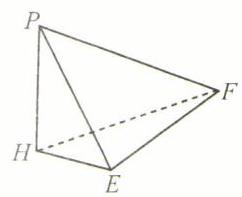
\includegraphics[width=0.2\textwidth]{bodyxb/src/bo_d20aucref24c73anc48g_142_1267_1894_242_197_0.jpg}
    \end{center}

    \xx{1}{2}{3}{4}
    \begin{jieda}
        不难判断, $\bigtriangleup {HEF},\bigtriangleup {PHE},\bigtriangleup {PHF}$ 均为直角三角形. 又 ${PH} \bot$ 平面 ${HEF} \Longrightarrow  {PH} \bot  {EF}$ ,而 ${EF} \bot  {HE} \cap$  ${PH} = H,\therefore {EF} \bot$ 平面 ${PHE},\therefore {EF} \bot  {PE}$ ,即 $\bigtriangleup  {PEF}$ 也是直角三角形.
    \end{jieda}
    
    \item 若两直线 $a$ 与 $b$ 异面,则过 $a$ 且与 $b$ 垂直的平面 \dotfill{(\kh{B})}
    \xx{有且只有一个}{可能存在也可能不存在}{有无数多个}{一定不存在}
    \begin{jieda}
        假设存在这样一个平面 $\alpha$ 满足要求, $\because b\bot \alpha ,a \subset  \alpha ,\therefore b\bot a$ . 因此 $a$ 与 $b$ 互相垂直是平面 $\alpha$ 存在的必要条件. 而当 $a\bot b$ 时,由 $a,b$ 的公垂线和 $a$ 确定的平面,即为 $\alpha$ . 
        
        当 $a\bot b$ 时,我们已说明了平面 $\alpha$ 的存在性,以下说明其唯一性. 假设平面 $\alpha ,\beta$ 均满足条件, $\alpha ,\beta$ 与直线 $b$ 交于相异两点 $A,B$ . 在直线 $a$ 上任取一点 $P$ ,则在平面 ${PAB}$ 中, ${PA}\bot b$ , ${PB} \bot  b$ ,矛盾. 故平面 $\alpha$ 是唯一的.
    \end{jieda}
    
    \item 从平面 $\alpha$ 外一点 $P$ 引与 $\alpha$ 相交的直线,使得点 $P$ 与交点的距离为 1,则满足条件的直线一定不可能是\dotfill{(\kh{C})}
    \xx{0 条}{1 条}{2 条}{无数条}
    \begin{jieda}
        记点 $P$ 与平面 $\alpha$ 的距离为 $d$ . 若 $d > 1$ ,则满足条件的直线不存在; 若 $d = 1$ ,则仅有一条; 若 $d < 1$ ,则有无数条.
    \end{jieda}
    
    \item 已知 $a,b$ 为异面直线,则下列命题正确的是\dotfill{(\kh{C})}
    \xx{过 $a,b$ 外一点 $P$ 一定可以引一条与 $a,b$ 都平行的直线}{过 $a,b$ 外一点 $P$ 一定可以作一个与 $a,b$ 都平行的平面}{过 $a$ 一定可以作一个与 $b$ 平行的平面}{过 $a$ 一定可以作一个与 $b$ 垂直的平面}

    \begin{jieda}
        对于选项 A, 若这样的直线存在, 由公理 4 可知: $a // b$, 与题设相悖, 错误; 对于选项 B, 当点P在过$a$且与$b$平行的直线上则无法实现, 错误; 对于选项 C,存在性: 在直线 $a$ 上任取一点 $P$ ,在直线 $b$ 上任取两点 $Q,R$ ,在平面 ${PQR}$ 中 (即点 $P$ 和直线 $b$ 确定的平面), 过点 $P$ 作直线 $b$ 的平行线 ${b}^{\prime }$ (可由尺规作图,构造平行四边形得到). 此时,相交直线 ${b}^{\prime }$ 和 $a$ 确定的平面即为与 $b$ 平行的平面 $\alpha$，正确; 对于选项 $D$，若$a$与$b$不垂直的时候无法实现，错误.
    \end{jieda}
    \item 已知 $M$ 是菱形 ${ABCD}$ 所在平面外一点,且 ${MA} = {MC}$ (如图),求证: ${AC} \bot$ 平面 ${BDM}$ .
    
    \begin{center}
    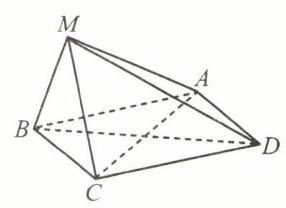
\includegraphics[width=0.2\textwidth]{bodyxb/src/bo_d20aucref24c73anc48g_143_1147_544_286_208_0.jpg}
    \end{center}
    \begin{jieda}
        设$AC, BD$交点为$O$，因为菱形对角线相互垂直平分，所以$AC \bot BD$，则因为$MA = MC$，所以$MO \bot AC$，$MO \cap BD = O$，故${AC} \bot$ 平面 ${BDM}$ .
    \end{jieda}
\end{enumerate}

\begin{center}  \textbf{(B)} \end{center}
\begin{enumerate}
    \item  已知直线 $a//$ 平面 $\alpha$ ,且 $a$ 与 $\alpha$ 之间的距离为 ${4m}\left( {m > 0}\right)$ ,那么到直线 $a$ 的距离与到平面 $\alpha$ 的距离都等于 ${3m}$ 的点的集合是\dotfill{(\kh{D})}
    \xx{一个平面}{两个相交平面}{一条直线}{两条平行直线}
    \begin{jieda}
        直观上看, 所求的点集, 是一个两端无限延伸的圆柱侧面, 被平行于该圆柱的轴的平面所截, 得到两条平行直线, 以下简要说明该结果. 如图,第 1 步:确定到平面 $\alpha$ 的距离都等于 ${3m}$ 的点的集合:位于平面 $\alpha$ 两侧, 与平面 $\alpha$ 平行且距离平面 $\alpha$ 为 ${3m}$ 的两个平面,所求点集只会在与直线 $a$ 在同侧的那个平面内,记作平面 $\beta$ ,且有 $\alpha //\beta$ ,直线 $a$ 到 $\beta$ 的距离为 $m$ . 第 2 步:确定平面 $\beta$ 内任意一点 $P$ 到直线 $a$ 的距离:直线 $a$ 在平面 $\beta$ 内的射影记为 ${a}^{\prime }$ ,作 ${PQ} \bot  {a}^{\prime }$ 于 $Q$ ; 在平行直线 $a,{a}^{\prime }$ 确定的平面内作 ${QR} \bot  a$ 于 $R$ ; 连接 ${PR}$ ,不难证明 ${a}^{\prime } \bot$ 平面 ${PQR},\therefore {a}^{\prime } \bot  {PR}$ ,
        
        \begin{center}
        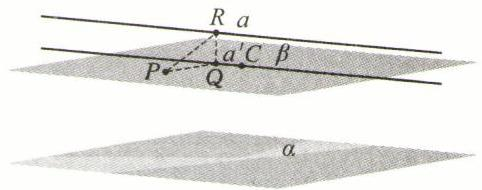
\includegraphics[width=0.3\textwidth]{bodyxb/src/bo_d20cdrf7aajc73bfmvhg_119_971_767_482_190_0.jpg}
        \end{center}
        
        $\therefore a\bot {PR}$ ,故线段 ${PR}$ 的长就是点 $P$ 到直线 $a$ 的距离, ${PR} = \sqrt{P{Q}^{2} + Q{R}^{2}} = \sqrt{P{Q}^{2} + {m}^{2}}$ . 第 3 步: 确定所求点集: 令 ${PR} = \sqrt{P{Q}^{2} + {m}^{2}} = {3m}$ ,求得 ${PQ} = 2\sqrt{2}m$ ,因此,所求点集是平面 $\beta$ 内到直线 ${a}^{\prime }$ 距离为 $2\sqrt{2}m$ 的两条平行直线.
    \end{jieda}
    \item \begin{enumerate}
        \item 已知 ${AB},{CD}$ 是两条不在同一个平面上的线段,且 ${AC} = {AD},{BC} = {BD}$ (如图),求证: ${AB}\bot {CD}$
        \begin{center}
        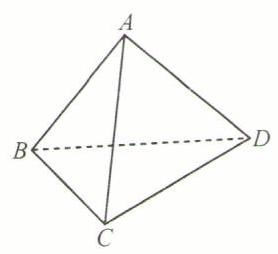
\includegraphics[width=0.2\textwidth]{bodyxb/src/bo_d20aucref24c73anc48g_143_417_1279_278_254_0.jpg}
        \end{center}
        \begin{jieda}
            取$CD$中点$O$，连接$AO, BO$，因为$AC = AD$，则$\triangle ACD$为等腰三角形，所以$AO \bot CD$，同理$BO \bot CD$，因此$CD \bot$ 平面$AOB$，故$AB \bot CD$.
        \end{jieda}
        \item 在空间四边形 ${ABCD}$ 中, $E$ , $F$ 分别为 ${AD}$ , ${BC}$ 的中点,若 ${AC} = {BD} = a,{EF} = \dfrac{\sqrt{2}}{2}a$ , $\angle {BDC} = {90}^{ \circ  }$ (如图),求证: ${BD} \bot$ 平面 ${ACD}$
        \begin{center}
        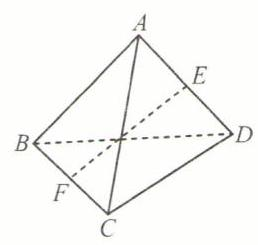
\includegraphics[width=0.2\textwidth]{bodyxb/src/bo_d20aucref24c73anc48g_143_953_1284_258_245_0.jpg}
        \end{center}
        \begin{jieda}
            取$CD$边中点$O$，连接$EO, FO$，根据三角形中位线定理可知$EO = FO = \dfrac{a}{2}$，故根据勾股定理逆定理可知$\angle{EOF}$为直角，即$EO \bot FO$，因此$EO \bot BD$，又因为$BD \bot CD$，$CD \cap EO = O$，所以${BD} \bot$ 平面 ${ACD}$
        \end{jieda}
        \item 在正方体 ${ABCD} - {A}_{1}{B}_{1}{C}_{1}{D}_{1}$ 中, $O$ 为底面 ${ABCD}$ 的中心, ${B}_{1}H \bot  {D}_{1}O$ , $H$ 是垂足 (如图),求证: ${B}_{1}H \bot$ 平面 $A{D}_{1}C$
        
        \begin{center}
        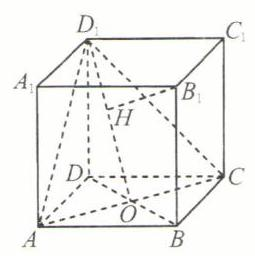
\includegraphics[width=0.2\textwidth]{bodyxb/src/bo_d20aucref24c73anc48g_143_435_1845_255_256_0.jpg}
        \end{center}
        \begin{jieda}
            因为$AC \bot BD, AC \bot BB_1$，故$AC \bot $平面$BB_1D_1D$，又因为$B_1H \subset $平面$BB_1D_1D$，因此$AC \bot B_1H$，又因为$B_1H \bot D_1O, D_1O \cap AC = O$，因此$B_1H \bot$ 平面 $A{D}_{1}C$
        \end{jieda}
        \item 在正方体 ${ABCD} - {A}_{1}{B}_{1}{C}_{1}{D}_{1}$ 中, $G$ 为 $C{C}_{1}$ 的中点, ${AC}$ 交 ${BD}$ 于点 $O$ (如图),求证: ${A}_{1}O \bot$ 平面 ${GBD}$
        \begin{center}
        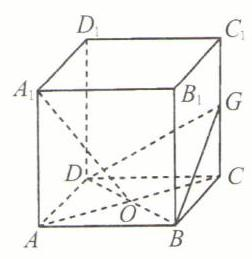
\includegraphics[width=0.2\textwidth]{bodyxb/src/bo_d20aucref24c73anc48g_143_948_1841_252_259_0.jpg}
        \end{center}
        \begin{jieda}
            $AC \bot BD, AA_1 \bot BD \Longrightarrow BD \bot $平面$ACC_1A_1 \Longrightarrow BD \bot A_1O$

            设立方体边长为$2$，则$A_1O = \sqrt{6}, OG = \sqrt{3}, A_1G = 3$，故$A_1O \bot OG$

            因为$A_1O \cap BD = O$故${A}_{1}O \bot$ 平面 ${GBD}$
        \end{jieda}
    \end{enumerate}
    \item 在 $\bigtriangleup {ABC}$ 中,已知 $\angle {ABC} = {90}^{ \circ  },{SA} \bot$ 平面 ${ABC}$ ,点 $A$ 在 ${SB},{SC}$ 上的射影分别为 $M,N$ (如图). 求证:

    \begin{enumerate*}
        \item ${BC} \bot$ 平面 ${SAB}$
        \item ${AM} \bot$ 平面 ${SBC}$
        \item ${SC} \bot  {MN}$
    \end{enumerate*}
    \begin{center}
    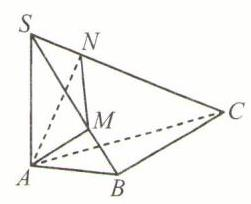
\includegraphics[width=0.2\textwidth]{bodyxb/src/bo_d20aucref24c73anc48g_144_425_483_251_204_0.jpg}
    \end{center}
    \begin{jieda}
        \begin{enumerate}
            \item 因为$\angle {ABC} = {90}^{ \circ  }$，所以$AB \bot BC$，因为${SA} \bot$ 平面 ${ABC}$，所以$SA \bot BC$，因此${BC} \bot$ 平面 ${SAB}$

            \item 由${BC} \bot$ 平面 ${SAB}$可知$BC \bot AM$，又因为$AM \bot SB$，所以${AM} \bot$ 平面 ${SBC}$

            \item 由${AM} \bot$ 平面 ${SBC}$可知$AM \bot SC$，又因为$AN \bot SC$，因此$SC \bot$ 平面$AMN$，因此${SC} \bot  {MN}$
        \end{enumerate}
    \end{jieda}
    \item 在正方体 ${ABCD} - {A}_{1}{B}_{1}{C}_{1}{D}_{1}$ 中,已知 $M,N$ 分别是棱 $A{A}_{1},{AB}$ 的中点, $P$ 为面对角线 ${B}_{1}{D}_{1}$ 的中点 (如图),求直线 ${PB}$ 和 ${MN}$ 所成的角.
    \begin{center}
    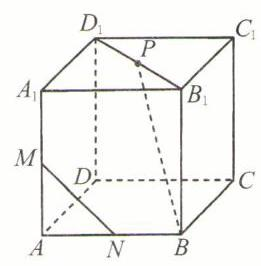
\includegraphics[width=0.2\textwidth]{bodyxb/src/bo_d20aucref24c73anc48g_144_936_419_261_266_0.jpg}
    \end{center}
    \begin{jieda}
        设正方体的单位棱长为 1.
        
        连接 ${A}_{1}B,{A}_{1}P$ ,易证 ${A}_{1}B//{MN}$ . 在 $\bigtriangleup {A}_{1}{BP}$ 中, ${A}_{1}B = \sqrt{2},{A}_{1}P = \dfrac{\sqrt{2}}{2},{BP} =$  $\sqrt{B{B}_{1}^{2} + {B}_{1}{P}^{2}} = \dfrac{\sqrt{6}}{2}$ . 由余弦定理, $\cos \angle {A}_{1}{BP} = \dfrac{{A}_{1}{B}^{2} + B{P}^{2} - {A}_{1}{P}^{2}}{2 \cdot  {A}_{1}B \cdot  {BP}} = \dfrac{\sqrt{3}}{2},\therefore {PB}$ 和 ${MN}$ 所成的角即为 $\angle {A}_{1}{BP} =$  ${30}^{ \circ  }$ . (或通过证明 ${A}_{1}P \bot$ 平面 ${DB}{B}_{1}{D}_{1} \Longrightarrow  {A}_{1}P \bot  {BP}$ ,无需求解 ${BP}$ 和余弦定理,有 $\sin \angle {A}_{1}{BP} = \dfrac{{A}_{1}P}{{A}_{1}B} = \dfrac{1}{2} \Longrightarrow  \angle {A}_{1}{BP} =$  $\left. {30}^{ \circ  }\right)$
    \end{jieda}
    \item 已知 $E,F$ 分别是正方形 ${ABCD}$ 边 ${AD},{AB}$ 的中点, ${EF}$ 交 ${AC}$ 于点 $M,{GC}$ 垂直于 ${ABCD}$ 所在平面 (如图).
    
    \begin{center}
    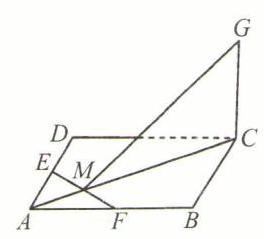
\includegraphics[width=0.2\textwidth]{bodyxb/src/bo_d20aucref24c73anc48g_144_1206_881_264_239_0.jpg}
    \end{center}
    \begin{enumerate}
        \item 求证: ${EF}\bot$ 平面 ${GMC}$
        \item 若 ${AB} = 4,{GC} = 2$ ,求点 $B$ 到平面 ${EFG}$ 的距离
    \end{enumerate}
    \begin{jieda}
        \begin{enumerate}
            \item 连接 ${BD}$ .
            
            $\left. \begin{array}{l} {EF}//{BD},{BD} \bot  {MC} \Longrightarrow  {EF} \bot  {MC}, \\  {GC} \bot  {ABCD} \Longrightarrow  {GC} \bot  {EF}, \\  {MC} \cap  {GC} = C \end{array}\right\}   \Longrightarrow  {EF} \bot$ 平面 ${GMC}$ ,证毕.
            \item 记 ${BD}$ 与 ${AC}$ 交于点 $O$ ,在平面 ${GMC}$ 中作 ${ON}\bot {MG}$ 于 $N$ . 
            
            第 1 步,证明 ${BD}//$ 平面 ${EFG}$ :由于 ${BD}//{EF}$ , ${BD}$ 和 ${EF}$ 分别在平面 ${EFG}$ 外和平面内, $\therefore {BD}//$ 平面 ${EFG}$ ,故 ${BD}$ 上任意一点 (这里取点 $O$ ) 到平面 ${EFG}$ 的距离即为所求. 
            
            第 2 步,证明 ${ON} \bot$ 平面 ${EFG}$ : 由 (1), ${EF} \bot$ 平面 ${GMC} \Longrightarrow  {EF} \bot  {ON}$ ,又 ${ON} \bot  {MG},{EF} \cap  {MG} = M$ ,$\therefore {ON} \bot$ 平面 ${EFG}$ . 
            
            第 3 步:求 ${ON}$ 的长:由 $\bigtriangleup  {ONM} \sim   \bigtriangleup  {GCM} \Longrightarrow  \dfrac{ON}{GC} = \dfrac{OM}{GM}$ ,其中 ${OM} = \dfrac{1}{4}{AC} = \dfrac{\sqrt{2}}{4}{AB} = \sqrt{2}$ , ${GM}$  $= \sqrt{C{M}^{2} + C{G}^{2}} = \sqrt{{\left( 3\sqrt{2}\right) }^{2} + {2}^{2}} = \sqrt{22}$ ,解得 ${ON} = \dfrac{2\sqrt{11}}{11}$ .
        \end{enumerate}
    \end{jieda}
    \item \begin{enumerate}
        \item 已知平面 $\alpha$ 和平面外的直线 $a$ 都垂直于直线 $b$ ,求证:平面 $\alpha$ 和直线 $a$ 互相平行
        \begin{jieda}
            记 $b \cap  \alpha  = A$ ,过 $b$ 上另一点 $P$ 作 ${a}^{\prime }//a$ ,再过 ${a}^{\prime }$ , $A$ 作平面 $\beta$ ,记 $\beta  \cap  \alpha  = {AB}$ ,则由 $b\bot \alpha$ 得 $b\bot {AB}$ ,又 $b\bot a$ , $\therefore b \bot  {a}^{\prime }$ . 于是 ${a}^{\prime }//{AB}$ ,故 $a//{AB}$ ,由此便得 $a//a$ .
        \end{jieda}
        \item 求证:经过一点 $A$ 和一条直线 $l$ 垂直的所有直线,都在经过点 $A$ 且垂直于直线 $l$ 的平面 $\alpha$ 内
        \begin{jieda}
            \ding{172}先证明 $A \in  l$ 的情况:假设存在一条经过点 $A$ 的直线 $m\bot l$ ,且 $m$ 不在平面 $\alpha$ 内,则相交直线 $m$ , $l$ 确定一个平面,记为 $\beta$ ; 根据公理3,平面 $\alpha ,\beta$ 的交线 ${m}^{\prime }$ 过点 $A$ ; 此时,在平面 $\beta$ 内,直线 $m$ 和 ${m}^{\prime }$ 均与直线 $l$ 垂直,矛盾,故不存在这样的直线 $m$ . \ding{173}再证明 $A \notin  l$ 的情况:此时,在点 $A$ 和 $l$ 确定的平面内,过点 $A$ 作 ${l}^{\prime }//l$ ,则 ${l}^{\prime }\bot$ 平面 $\alpha$ . 类似地, 如果存在一条经过点 $A$ 的直线 $m\bot l \Longrightarrow  m\bot {l}^{\prime }$ ,且 $m$ 不在平面 $\alpha$ 内,则将\ding{172}的证明中,所有的 $l$ 改写成 ${l}^{\prime }$ ,同样推得矛盾. 综上,所有满足题意的直线均在平面 $\alpha$ 内,证毕.
        \end{jieda}
    \end{enumerate}

\end{enumerate}
\subsection*{(三) 三垂线定理}

\subsubsection*{【典型题型和解题技巧】}

1. \textbf{三垂线定理} 

平面上的一条直线和这个平面的一条斜线垂直的充要条件是它和这条斜线在平面上的投影垂直.

2. 三垂线定理的应用.

(1)证明线线垂直.

\textbf{例 1} 在四面体 ${ABCD}$ 中,已知 ${AB} \bot  {CD},{AC} \bot  {BD}$ . 求证: ${AD} \bot  {BC}$ .

\begin{center}
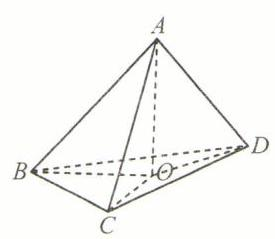
\includegraphics[width=0.2\textwidth]{bodyxb/src/bo_d20aucref24c73anc48g_144_1217_1789_275_239_0.jpg}
\end{center}

\textbf{分析} 

要证明 ${AD} \bot  {BC}$ ,根据三垂线定理,只需证明 ${AD}$ 在平面 ${BCD}$ 内的射影和 ${BC}$ 垂直,因此,可作 ${AO} \bot$ 平面 ${BCD}$ 于点 $O$ ,问题即转化为证明 ${OD} \bot  {BC}$ .

\textbf{证明} 

如图，作 ${AO} \bot$ 平面 ${BCD}$ 于点 $O$ ,连接 ${BO},{CO},{DO}$ ,则 ${BO}$ , ${CO},{DO}$ 分别为 ${AB},{AC},{AD}$ 在平面 ${BCD}$ 上的射影.

$\because {AB} \bot  {CD}$ , $\therefore {BO} \bot  {CD}$ (三垂线定理),同理 ${CO} \bot  {BD}$ . 于是 $O$ 是 $\bigtriangleup  {BCD}$ 的垂心.

$\therefore {DO} \bot  {BC}$ ,于是 ${AD} \bot  {BC}$ (三垂线定理).

\textbf{注意 运用三垂线定理的关键在于确定斜线在平面上的射影,而射影确定的关键又是“垂足”,如果“垂足”定了,那么“垂足”和“斜足”的连线就是斜线在平面上的射影.}

(2)求点到直线的距离.

\textbf{例 2} 已知 ${PA} \bot$ 正六边形 ${ABCDEF}$ 所在平面,且 ${PA} = a,{AB} = b$ ,如图(1),求点 $P$ 到边 ${BC},{CD}$ 的距离.

\begin{center}
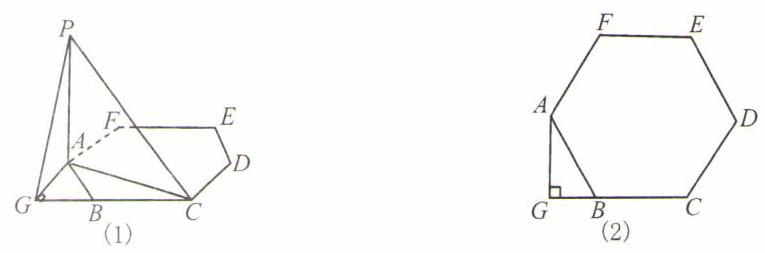
\includegraphics[width=0.6\textwidth]{bodyxb/src/bo_d20aucref24c73anc48g_145_386_596_765_253_0.jpg}
\end{center}

\textbf{解} 

过点 $A$ 作直线 ${CB}$ 的垂线,与 ${CB}$ 的延长线交于点 $G$ ,连接 ${PG}$ ,则 ${PG} \bot  {CB}$ (三垂线定理),所以 ${PG}$ 就是 $P$ 到边 ${BC}$ 的距离,连接 ${AC},{PC}$ .

$\because {ABCDEF}$ 是正六边形, $\therefore {AC} \bot  {CD}$ ,于是 ${PC} \bot  {CD}$ (三垂线定理),

$\therefore {PC}$ 就是点 $P$ 到边 ${CD}$ 的距离.

如图(2), $\because {AB} = b$ ,则 ${AG} = \dfrac{\sqrt{3}}{2}b,{AC} = \sqrt{3}b$ ,

$\therefore {PG} = \sqrt{{a}^{2} + \dfrac{3}{4}{b}^{2}} = \dfrac{1}{2}\sqrt{4{a}^{2} + 3{b}^{2}},{PC} = \sqrt{{a}^{2} + 3{b}^{2}}$ ,

即点 $P$ 到边 ${BC},{CD}$ 的距离分别为 $\dfrac{1}{2}\sqrt{4{a}^{2} + 3{b}^{2}}$ 和 $\sqrt{{a}^{2} + 3{b}^{2}}$ .

注意(1)对于立体几何中的计算题,可按“作,证,算”三步进行:第一步是“作”,先作出欲求的线段,欲求的角；第二步是 “证”,证明所作的线段或角符合题目要求；第三步是 “算”,根据已知条件进行计算.

(2)立体几何中很多图形由于位置关系,与 “真形”(即平面图形)有 “差距”,为了能正确地确定线段之间的数量关系或位置关系,可以另外画出“真形”.

如本例,画出了正六边形的“真形”[如图(2)]后,就易得 $\angle {ABG} = {60}^{ \circ  },{AC} \bot  {CD}$ .

\subsubsection*{【训练题】}

\begin{center}  \textbf{(A)} \end{center}

\begin{enumerate}
    \item 若平面外一条直线和这个平面所成角是 $\theta$ ,则 $\theta$ 的取值范围是\dotfill{(\kh{D})}
    \xx{${0}^{ \circ  } < \theta  < {180}^{ \circ  }$}{${0}^{ \circ  } < \theta  < {90}^{ \circ  }$}{${0}^{ \circ  } < \theta  \leq {90}^{ \circ  }$}{${0}^{ \circ  } \leq  \theta  \leq  {90}^{ \circ  }$}
    \begin{jieda}
        根据定义,当直线与平面平行(或在平面内)时, $\theta  = {0}^{ \circ  }$ ；当直线与平面垂直时, $\theta  = {90}^{ \circ  }$ ；其余情况,直线和平面所成的角,是该直线与它在平面上的射影所成的锐角.
    \end{jieda}
    \item 在正方体 ${EFGH} - {E}_{1}{F}_{1}{G}_{1}{H}_{1}$ 中, ${O}_{1}$ 是 ${E}_{1}{F}_{1}{G}_{1}{H}_{1}$ 的中心 (如图), 则与 $F{G}_{1}$ 与对角面 $F{F}_{1}{H}_{1}H$ 所成角的大小相等的是\dotfill{(\kh{B})}
    
    \begin{center}
    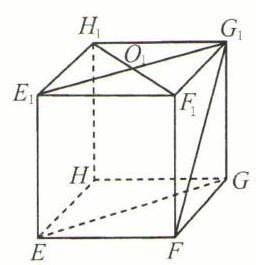
\includegraphics[width=0.2\textwidth]{bodyxb/src/bo_d20aucref24c73anc48g_146_1214_133_256_265_0.jpg}
    \end{center}
    \xx{$\angle {G}_{1}F{H}_{1}$}{$\angle {G}_{1}F{O}_{1}$}{$\angle {G}_{1}F{F}_{1}$}{$\angle {G}_{1}{FH}$}
    \begin{jieda}
        点 $F,{G}_{1}$ 分别在平面 $F{F}_{1}{H}_{1}H$ 内,外. 又 ${G}_{1}{O}_{1} \bot  {H}_{1}{F}_{1},{G}_{1}{O}_{1} \bot  {H}_{1}H,\therefore {G}_{1}{O}_{1} \bot$ 平面 $F{F}_{1}{H}_{1}H$，$\therefore$ 点 ${G}_{1}$ 在平面 $F{F}_{1}{H}_{1}H$ 内的射影是点 ${O}_{1}$ ,故 $F{G}_{1}$ 与平面 $F{F}_{1}{H}_{1}H$ 所成的角是 $\angle {G}_{1}F{O}_{1}$ . 由于点在平面内射影的唯一性,其他选项均不可能.
    \end{jieda}
    
     \item 若平面 $\alpha$ 外两直线 $a,b$ 在 $\alpha$ 上的射影是两相交直线,则 $a$ 与 $b$ 的位置关系是 \dotfill{(\kh{B})}
     \xx{相交}{相交或异面}{异面}{相交或平行}
     \begin{jieda}
         在正方体 ${ABCD} - {A}^{\prime }{B}^{\prime }{C}^{\prime }{D}^{\prime }$ 中,取 $\alpha  =$ 平面 ${ABCD}$ ,相交直线 $a = {A}^{\prime }{C}^{\prime },b = {B}^{\prime }{D}^{\prime }$ 或异面直线 $a = {A}^{\prime }{C}^{\prime },b = {BC}$ 在 $\alpha$ 上的射影都是两相交直线. $a$ 与 $b$ 不可能互相平行,简证如下: (反证法) 假设 $a//b$ ,且 $a,b$ 在平面 $\alpha$ 内的射影 $m,n$ 交于点 $O$ ,过点 $O$ 作平面 $\alpha$ 的垂线 $l$ ,则 $a$ , $b$ 和 $l$ 都有交点,记 $b \cap  l = N.l$ , $m$ 确定的平面为 $\beta$ ,则 $a \subset  \beta$ ,又 $b \not \subset \beta$ 且 $a//b$ ,故 $b$  $//\beta$ ,然而 $N \in  b,N \in  l \subset  \beta$ ,故矛盾,因此 $a//b$ 不成立,证毕. 综上, $a$ 与 $b$ 相交或异面.
     \end{jieda}
     
      \item 已知 $P$ 是 $\bigtriangleup {EFG}$ 所在平面外一点,且 ${PE} = {PG}$ ,则点 $P$ 在面 ${EFG}$ 上的射影一定在 $\bigtriangleup  {EFG}$ 的\dotfill{(\kh{D})}
      \xx{$\angle {FEG}$ 的平分线上}{边 ${EG}$ 的高上}{边 ${EG}$ 的中线上}{边 ${EG}$ 的垂直平分线上}
      \begin{jieda}
          设点 $P$ 在面 ${EFG}$ 上的射影是点 $O$ ,在 ${{Rt}} \bigtriangleup  {POE}$ 和 ${{Rt}} \bigtriangleup  {POG}$ 中,由勾股定理,易得: ${PE} = {PG} \Longrightarrow  {OE} = {OG}$ ,即点 $O$ 在边 ${EG}$ 的垂直平分线上.
      \end{jieda}
      
      \item 从平面 $\alpha$ 外一点 $P$ 向 $\alpha$ 引垂线和若干条斜线,若这些斜线与 $\alpha$ 所成的角都相等,则\dotfill{(\kh{C})}
      \xx{斜足一定是一正多边形的顶点}{垂足是以斜足为顶点的多边形的内心}{垂足是以斜足为顶点的多边形的外心}{垂足是以斜足为顶点的多边形的垂心}
      \begin{jieda}
          由题意,垂线、斜线段及其对应的射影构成的三角形均全等,故垂足到各个斜足的距离均相等,换言之:垂足在任意两斜足连线段的垂直平分线上,故垂足是以斜足为顶点的多边形的外心.
      \end{jieda}
      \item \begin{enumerate}
          \item 已知 ${PA}$ 垂直于 $\bigtriangleup  {ABC}$ 所在平面,且 ${AB} = {AC} = {13},{BC} = {10},{PA} = {12}$ ,则 $P$ 到 ${BC}$ 的距离等于\blkda{${12}\sqrt{2}$}
          \begin{jieda}
              作 ${AD}\bot {BC}$ 于 $D$ ,连接 ${PD}$ . 不难求得 ${AD} = {12}$ . 又 ${PD}$ 在平面 ${ABC}$ 上的射影是 ${AD}$ ,根据三垂线定理, ${BC} \bot  {AD} \Longrightarrow  {BC} \bot  {PD}$ ,故 $P$ 到 ${BC}$ 的距离即为 ${PD} = \sqrt{P{A}^{2} + D{A}^{2}} = {12}\sqrt{2}$ .
          \end{jieda}
          \item 已知 ${PA}$ 垂直于正六边形 ${ABCDEF}$ 所在平面,且 ${PA} = 1$ ,边长 ${AB} = 2$ ,则点 $P$ 到边 ${BC}$ 的距离等于\blkda{2}
          \begin{jieda}
              作 ${AG} \bot  {CB}$ 的延长线于 $G$ ,连接 ${PG}$ . 不难求得 ${AG} = \sqrt{3}$ . 又 ${PG}$ 在正六边形 ${ABCDEF}$ 所在平面上的射影是 ${AG}$ ,根据三垂线定理, ${CB} \bot  {AG} \Longrightarrow  {CB} \bot  {PG}$ ,故 $P$ 到 ${BC}$ 的距离即为 ${PG} = \sqrt{P{A}^{2} + G{A}^{2}} = 2$ .
          \end{jieda}
          \item 过平面 $\alpha$ 外一点 $P$ 引 $\alpha$ 的垂线 ${PO}$ 与斜线 ${PA},{PB}(O,A,B$ 为垂足与斜足),若 ${PA} =$  $8{{cm}},{PB} = 5{{cm}}$ ,又 ${OA} : {OB} = 4 : \sqrt{3}$ ,则点 $P$ 到 $\alpha$ 的距离等于\blkda{4} ${{cm}}$
          \begin{jieda}
              设点 $P$ 到 $\alpha$ 的距离 ${PO} = h {{cm}}$ ,并设 ${OA} = {4k}{{cm}},{OB} = \sqrt{3}k {{cm}}\left( {h,k > 0}\right)$ . 在Rt $\bigtriangleup  {POA}$ 和 Rt $\bigtriangleup  {POB}$ 中,由勾股定理得 $\left\{  \begin{array}{l} {h}^{2} + {16}{k}^{2} = {64}, \\  {h}^{2} + 3{k}^{2} = {25}. \end{array}\right.$ 解得 $\left\{  \begin{array}{l} h = 4 \\  k = \sqrt{3} \end{array}\right.$ .
          \end{jieda}
      \end{enumerate}
      \item 已知 ${SA}$ 垂直于直角三角形 ${ABC}$ 所在平面, $\angle {ABC} = {90}^{ \circ  },B{B}_{1}\bot {AC}$ 于点 ${B}_{1}$ ,则:
      \begin{enumerate}
          \item ${SA},{SB},{SC}$ 在平面 ${ABC}$ 上的射影依次是\blkda[3]{点 $A\text{ 、 }{AB}\text{ 、 }{AC}$}
          \item ${CA},{CB},{CS}$ 在平面 ${SAB}$ 上的射影依次是\blkda[3]{${BA}$ 、点 $B$ 、 ${BS}$}
          \item ${BA},{BC},{BS}$ 在平面 ${SAC}$ 上的射影依次是\blkda[3]{${B}_{1}A$ 、 ${B}_{1}C$ 、 ${B}_{1}S$}
      \end{enumerate}
      \item 已知 $P$ 为 $\bigtriangleup {ABC}$ 所在平面外一点,且在平面 ${ABC}$ 上的射影为 $O$ .
      \begin{enumerate}
          \item 若 ${PA} = {PB} = {PC}$ ,则 $O$ 为 $\bigtriangleup  {ABC}$ 的\blkda{外}心,又若 $\angle {ACB} = {90}^{ \circ  }$ ,则 $O$ 在\blkda[2.5]{边 ${AB}$ 的中点}
          \begin{jieda}
              ${PA} = {PB} = {PC} \Longrightarrow  {OA} = {OB} = {OC}$ ,故 $O$ 为 $\bigtriangleup  {ABC}$ 的外心；又直角三角形的外心在斜边的中点,故 $\angle {ACB} = {90}^{ \circ  }$ 时, $O$ 在边 ${AB}$ 的中点.
          \end{jieda}
          \item 若 ${PA},{PB},{PC}$ 与平面 ${ABC}$ 所成的角相等,则 $O$ 为 $\bigtriangleup  {ABC}$ 的\blkda{外}心
          \begin{jieda}
              由题意, $\bigtriangleup {PAO}$ , $\bigtriangleup {PBO}$ , $\bigtriangleup {PCO}$ 是全等三角形,故 ${OA} = {OB} = {OC}$ , $O$ 为 $\bigtriangleup {ABC}$ 的外心.
          \end{jieda}
          \item 若 $O$ 在 $\bigtriangleup {ABC}$ 内,且 $P$ 到 $\bigtriangleup {ABC}$ 的三边距离相等,则 $O$ 为 $\bigtriangleup {ABC}$ 的\blkda{内}心
          \begin{jieda}
              过点 $O$ 作 $\bigtriangleup {ABC}$ 三边 ${AB},{BC},{CA}$ 的垂线,垂足分别为 $D,E,F$ . 由三垂线定理,点 $P$ 到 $\bigtriangleup {ABC}$ 三边 ${AB}$ 、 ${BC}\text{ 、 }{CA}$ 的距离就是 ${PD},{PE},{PF}\text{ 、 }{PD} = {PE} = {PF} \Longrightarrow  {OD} = {OE} = {OF}$ ,又 $O$ 在 $\bigtriangleup {ABC}$ 内,故 $O$ 为 $\bigtriangleup {ABC}$ 的内心. (注: 若不限定 $O$ 在 $\bigtriangleup {ABC}$ 内,则 $O$ 为 $\bigtriangleup {ABC}$ 的内心或旁心)
          \end{jieda}
          \item 若四面体 ${PABC}$ 的两组对棱互相垂直,则 $O$ 为 $\bigtriangleup  {ABC}$ 的\blkda{垂}心
          \begin{jieda}
              连接 ${AO}$ ,它是 ${AP}$ 在平面 ${ABC}$ 上的射影. 由三垂线定理, ${PA} \bot  {BC} \Longrightarrow  {AO} \bot  {BC}$ . 同理 ${CO} \bot  {AB}$ 、 ${BO} \bot  {AC}$ , 故 $O$ 为 $\bigtriangleup {ABC}$ 的垂心.
          \end{jieda}
      \end{enumerate}
      \item \begin{enumerate}
          \item 在长方体 ${ABCD} - {A}_{1}{B}_{1}{C}_{1}{D}_{1}$ 中,棱 ${AB},{AD},A{A}_{1}$ 的长分别为6,8,3.6,则 $A$ 到 ${B}_{1}{D}_{1}$ 的距离为\blkda{6}
          \begin{jieda}
              在平面 $A{B}_{1}{D}_{1}$ 中,作 ${AE}\bot {B}_{1}{D}_{1}$ 于 $E$ ,连接 ${A}_{1}E$ . 显然, ${AE}$ 在平面 ${A}_{1}{B}_{1}{C}_{1}{D}_{1}$ 上的射影是 ${A}_{1}E$ ,由三垂线定理, ${AE} \bot  {B}_{1}{D}_{1} \Longrightarrow  {A}_{1}E \bot  {B}_{1}{D}_{1}$ . 由面积法 (或相似三角形), ${A}_{1}E = \dfrac{{A}_{1}{D}_{1} \cdot  {A}_{1}{B}_{1}}{{B}_{1}{D}_{1}} = {4.8}$ ,故 ${AE} =$  $\sqrt{{A}_{1}{A}^{2} + {A}_{1}{E}^{2}} = 6$ ,即为所求.
          \end{jieda}
          \item 在矩形 ${ABCD}$ 中,已知 ${AB} = b,{AD} = c$ ,线段 ${PA}\bot$ 矩形 ${ABCD}$ 所在平面,且 ${PA} =$  $a$ ,则 $\bigtriangleup  {PBD}$ 的面积是\blkda[3.5]{$\dfrac{1}{2}\sqrt{{a}^{2}{b}^{2} + {b}^{2}{c}^{2} + {c}^{2}{a}^{2}}$}
          \begin{jieda}
              在平面 ${PBD}$ 中,作 ${PE}\bot {BD}$ 于 $E$ ,连接 ${AE}$ . 显然, ${PE}$ 在平面 ${ABCD}$ 上的射影是 ${AE}$ ,由三垂线定理, ${PE} \bot  {BD} \Longrightarrow  {AE} \bot  {BD}$ . 由面积法 (或相似三角形), ${AE} = \dfrac{{AD} \cdot  {AB}}{BD} = \dfrac{bc}{\sqrt{{b}^{2} + {c}^{2}}}$ ,故 ${PE} =$  $\sqrt{A{P}^{2} + A{E}^{2}} = \sqrt{\dfrac{{a}^{2}{b}^{2} + {b}^{2}{c}^{2} + {c}^{2}{a}^{2}}{{b}^{2} + {c}^{2}}}$ ,故 ${S}_{\bigtriangleup {PBD}} = \dfrac{1}{2} \cdot  {BD} \cdot  {PE} = \dfrac{1}{2}\sqrt{{a}^{2}{b}^{2} + {b}^{2}{c}^{2} + {c}^{2}{a}^{2}}$
          \end{jieda}
          \item 在棱长为 $a$ 的正方体 ${ABCD} - {A}_{1}{B}_{1}{C}_{1}{D}_{1}$ 中, ${D}_{1}$ 到 ${B}_{1}C$ 的距离为\blkda{$\dfrac{\sqrt{6}}{2}a$}, $A$ 到 ${A}_{1}C$ 的距离为\blkda{$\dfrac{\sqrt{6}}{3}a$}
          \begin{jieda}
              $\bigtriangleup {D}_{1}{B}_{1}C$ 是边长为 $\sqrt{2}a$ 的等边三角形,故 ${D}_{1}$ 到 ${B}_{1}C$ 的距离为 $\dfrac{\sqrt{3}}{2} \cdot  \sqrt{2}a = \dfrac{\sqrt{6}}{2}a.\operatorname{Rt} \bigtriangleup  {A}_{1}{AC}$ 中, $\angle {A}_{1}{AC} = {90}^{ \circ  }$ ,由面积法 (或相似三角形), $A$ 到 ${A}_{1}C$ 的距离为 $\dfrac{A{A}_{1} \cdot  {AC}}{{A}_{1}C} = \dfrac{a \cdot  \sqrt{2}a}{\sqrt{3}a} = \dfrac{\sqrt{6}}{3}a.$
          \end{jieda}
          \item 在菱形 ${ABCD}$ 中,已知 $\angle {BAD} = {60}^{ \circ  },{AB} = {10}{{cm}},{PA}\bot$ 菱形 ${ABCD}$ 所在平面,且 ${PA} = {5{{cm}}}$ ,则 $P$ 到 ${BD}$ 的距离为\blkda{10} ${{cm}}$ , $P$ 到 ${DC}$ 的距离为\blkda{10} ${{cm}}$
          \begin{jieda}
              连接 ${AC},{BD}$ 交于点 $E$ ,连接 ${PE}.{AE}$ 是 ${PE}$ 在平面 ${ABCD}$ 上的射影,由三垂线定理, ${BD}\bot {AE} \Longrightarrow  {BD}$  $\bot {PE}.\bigtriangleup {ABD}$ 是等边三角形,故 ${AE} = 5\sqrt{3}{{cm}},P$ 到 ${BD}$ 的距离 ${PE} = \sqrt{A{P}^{2} + A{E}^{2}} = {10}{{cm}}$ . 作 ${AF}\bot {CD}$ 延长线于点 $F$ ,连接 ${PF}.{AF}$ 是 ${PF}$ 在平面 ${ABCD}$ 上的射影,由三垂线定理, ${AF} \bot  {CD} \Longrightarrow  {PF} \bot  {CD}$ . 不难求得, ${AF} = {AE} = 5\sqrt{3}$  ${{cm}}$ ,故 $P$ 到 ${DC}$ 的距离 ${PF} = {PE} = {10}{{cm}}$ .
          \end{jieda}
      \end{enumerate}
      \item \begin{enumerate}
          \item 若 ${{Rt}}\bigtriangleup {ABC}$ 所在平面外一点 $P$ 到点 $A,B,C$ 等距离,点 $P$ 到面 ${ABC}$ 的距离为 $b$ ,且一直角边长为 ${2a}$ ,则 $P$ 到另一直角边的距离等于\blkda{$\sqrt{{a}^{2} + {b}^{2}}$}
          \begin{jieda}
              不妨设 $\angle {ACB} = {90}^{ \circ  },{BC} = {2a}$ . 点 $P$ 在平面 ${ABC}$ 上的射影是点 $O$ ,由第 85(1) 题的讨论,可知 $O$ 为边 ${AB}$ 的中点. 取 ${AC}$ 的中点 $D$ ,连接 ${OD}$ , ${PD}$ . 由三角形的中位线定理,可知 ${OD} = a$ ,且 ${OD}//{BC} \Longrightarrow  {OD} \bot  {AC}$ ,再由三垂线定理, ${PD} \bot  {AC}$ ,故 ${PD} = \sqrt{{a}^{2} + {b}^{2}}$ 即为所求.
          \end{jieda}
          \item 正方体 ${ABCD} - {A}_{1}{B}_{1}{C}_{1}{D}_{1}$ 的棱长为 $a$ ,则顶点 $B$ 到截面 ${AC}{B}_{1}$ 的距离是\blkda{$\dfrac{\sqrt{3}}{3}a$}
          \begin{jieda}
              截面 ${AC}{B}_{1}$、截面 ${A_1C_1}D$三等分体对角线$BD_1$，且$BD_1$垂直于两截面.
          \end{jieda}
          \item $P$ 为 $\bigtriangleup  {ABC}$ 所在平面 $\alpha$ 外一点,且 ${PA} = {PB} = {PC} = {10},{AB} = 6,{BC} = 8,{CA} = {10}$ ,则点 $P$ 到平面 ${ABC}$ 的距离为\blkda{$5\sqrt{3}$}, ${PA},{PB},{PC}$ 与面 ${ABC}$ 所成的三个角依次为\blkda[2]{${60}^{ \circ  },{60}^{ \circ  },{60}^{ \circ  }$}
          \begin{jieda}
              $\angle{B} = \ang{90}$，$P$在$\alpha$内的射影是$AC$中点.
          \end{jieda}
      \end{enumerate}
      \item \begin{enumerate}
          \item 若线段 ${AB}$ 和平面 $\alpha$ 成 ${30}^{ \circ  }$ 角, $A$ , $B$ 与平面 $\alpha$ 的距离分别是 $6{{cm}}$ 和 ${10}{{cm}}$ ,则 ${AB}$ 的长是\blkda{8 或 32} ${{cm}}$
          \begin{jieda}
              记直线 ${AB}$ 与平面 $\alpha$ 交于点 $O$ ,则 ${OA} = \dfrac{6}{\sin {30}^{ \circ  }} = {12}{{cm}},{OB} = \dfrac{10}{\sin {30}^{ \circ  }} = {20}{{cm}}$ . 当 $A,B$ 在平面 $\alpha$ 同侧时, ${AB} = {20} - {12} = 8{{cm}}$ ; 当 $A,B$ 在平面 $\alpha$ 异侧时, ${AB} = {20} + {12} = {32}{{cm}}$
          \end{jieda}
          \item 在平面 $\alpha$ 的一侧有一个三角形,三个顶点至平面 $\alpha$ 的距离分别是9,5,5,则这个三角形的重心到 $\alpha$ 的距离为\blkda{$\dfrac{19}{3}$}
          \begin{jieda}
              过距离为5的顶点做与$\alpha$平行的平面$\beta$，则三个顶点到$\beta$的距离为$4,0,0$（设为$A,B,C$），连接$A$和重心$O$，交$BC$于$D$，做$A,O$在$\beta$内的射影$A', O'$，则$\bigtriangleup{AA'D} \sim \bigtriangleup{OO'D}$，因此$OO' = \dfrac{1}{3}AA' = \dfrac{4}{3}$，因此$O$到$\alpha$的距离为$\dfrac{4}{3}+5 = \dfrac{19}{3}$
          \end{jieda}
          \item 平面 $\alpha$ 外两点 $A,B$ 到 $\alpha$ 的距离分别为 $a,b,P$ 是线段 ${AB}$ 上一点,且 ${AP} : {PB} = 1: 2$，则 $P$ 到平面 $\alpha$ 的距离是\blkda[3]{$\dfrac{{2a} + b}{3}$ 或 $\dfrac{\left| {2a} - b\right| }{3}$}
          \begin{jieda}
              在 ${AB}$ 和它在平面 $\alpha$ 上的射影 ${A}^{\prime }{B}^{\prime }$ 确定的平面内,将问题转化为点 $P$ 到 ${A}^{\prime }{B}^{\prime }$ 的距离问题 (平面几何). 当 $A,B$ 在平面 $\alpha$ 同侧时,所求距离为 $a + \dfrac{1}{3}\left( {b - a}\right)  = \dfrac{{2a} + b}{3}$ ; 当 $A,B$ 在平面 $\alpha$ 异侧时,所求距离为 $\left| {a - \dfrac{1}{3}\left( {a + b}\right) }\right|  = \dfrac{\left| 2a - b\right| }{3}.$
          \end{jieda}
      \end{enumerate} 
      \item 在正方体 ${ABCD} - {A}_{1}{B}_{1}{C}_{1}{D}_{1}$ 中,\begin{enumerate}
          \item 若 $O,{O}_{1}$ 分别为 ${ABCD},{A}_{1}{B}_{1}{C}_{1}{D}_{1}$ 的中心,则异面直线 ${A}_{1}O$ 与 $D{O}_{1}$ 所成角的余弦值为\blkda{$\dfrac{2}{3}$}
          \begin{jieda}
              设正方形边长为 1 .连接 ${O}_{1}C$ . 由 ${A}_{1}{O}_{1}$与$ {OC}$平行且相等 ,可知四边形 ${A}_{1}{O}_{1}{CO}$ 为平行四边形,故 ${A}_{1}O$与${O}_{1}C$平行且相等 在 $\bigtriangleup  {O}_{1}{CD}$ 中, ${O}_{1}D =$  ${O}_{1}C = \dfrac{\sqrt{6}}{2},{CD} = 1$ ,由余弦定理得 $\cos \angle D{O}_{1}C = \dfrac{{O}_{1}{D}^{2} + {O}_{1}{C}^{2} - C{D}^{2}}{2 \cdot  {O}_{1}D \cdot  {O}_{1}C} = \dfrac{2}{3}$ .
          \end{jieda}
          \item 若 $E,F,G,H$ 分别是 ${AB},{B}_{1}{C}_{1},{BC},{C}_{1}{D}_{1}$ 的中点,则 ${EF}$ 与 ${GH}$ 所成角的余弦值为\blkda{$\dfrac{2}{3}$}
          \begin{jieda}
              平移后可与上一题一致.
          \end{jieda}
      \end{enumerate}
\end{enumerate}
\begin{center}  \textbf{(B)} \end{center}
\begin{enumerate}
    \item 已知直线 $a$ 是与平面 $\alpha$ 成 $\theta$ 角的一条斜线, $b$ 是 $\alpha$ 上与 $a$ 异面的任意一条直线,则 $a$ 与 $b$ 所成角\dotfill{(\kh{A})}
    \xx{有最小值 $\theta$ ,也有最大值 $\dfrac{\pi }{2}$}{有最小值 $\theta$ ,也有最大值 $\pi$}{有最小值 $\theta$ ,但没有最大值}{没有最小值,但有最大值 $\dfrac{\pi }{2}$}
    \begin{jieda}
        记 $a \cap$ 平面 $\alpha  = O$ . 显然,平面 $\alpha$ 内任意一条不经过点 $O$ 的直线,都与直线 $a$ 异面. 过点 $O$ 作 ${b}^{\prime }//b$ . 根据最小角定理,当 ${b}^{\prime }$ 取 $a$ 在平面 $\alpha$ 上的射影时,平面 $\alpha$ 内任意与直线 ${b}^{\prime }$ 平行的直线,都能使 $a$ 与 $b$ 所成角最小,最小值为 $\theta$ ；根据三垂线定理,当 ${b}^{\prime }$ 垂直于 $a$ 在平面 $\alpha$ 上的射影时,平面 $\alpha$ 内任意与直线 ${b}^{\prime }$ 平行的直线,都能使 $a$ 与 $b$ 所成角最大,最大值为 $\dfrac{\pi }{2}$ . 
        
        \ps 最小角定理: 斜线与平面所成的角,是这条斜线与平面内经过斜足的任意直线所成的角中最小的角. （证明见下一题注释）
    \end{jieda}
    \item 已知直线 ${PA},{PB},{PC}$ 两两相交成直角,一平面与 ${PA},{PB},{PC}$ 分别相交于点 $A,B,C$ ,则 $\bigtriangleup {ABC}$ 的形状一定是\dotfill{(\kh{B})}
    \xx{直角三角形}{锐角三角形}{钝角三角形}{锐角三角形或钝角三角形}
    \begin{jieda}
        如图,作 ${PD}\bot {BC}$ 于 $D$ ,连接 ${AD}$ . 由题意, ${AP}\bot$ 平面 ${BPC}$ ,故斜线 ${AC},{AD}$ 在平面 ${BPC}$ 上的射影是 ${PC},{PD}$ ,由三垂线定理, ${AD} \bot  {BC}.\cos \angle {ACB} = \dfrac{DC}{AC} = \dfrac{DC}{PC} \cdot  \dfrac{PC}{AC} = \cos \angle {PCD}$ . $\cos \angle {PCA}$ ,而 $\angle {PCD},\angle {PCA}$ 必为锐角,故 $\angle {ACB}$ 也是锐角. 同理, $\bigtriangleup {ABC}$ 的三个角都是锐角. 
        \begin{center}
        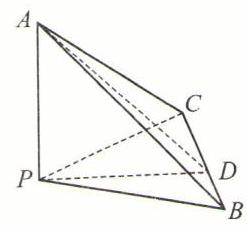
\includegraphics[width=0.2\textwidth]{bodyxb/src/bo_d20cdrf7aajc73bfmvhg_122_1287_1612_247_227_0.jpg}
        \end{center}

        \ps 三面角余弦定理：$cos\angle{ACB} = cos\angle{ACP} \cdot cos\angle{BCP}+sin\angle{ACP}\cdot sin\angle{BCP} \cdot cos\angle{APB}$，因为二面角的平面角$\angle{APB}$为直角，所以简化为$cos\angle{ACB} = cos\angle{ACP} \cdot cos\angle{BCP}$
        
        \ps 对于锐角 $\angle {ACB}$ 和 $\angle {ACP}$，$cos\angle{ACB} = cos\angle{ACP} \cdot cos\angle{BCP} \leq cos \angle{ACP}$，当且仅当$C,P,B$共线时取等，故$\angle {ACB} \geq \angle {ACP}$，最小角定理证毕.
    \end{jieda}
    \item 已知 $P$ 是四边形 ${ABCD}$ 所在平面外一点,且 $P$ 到这四边形各边的距离相等,那么这个四边形一定是 \dotfill{(\kh{C})}
    \xx{圆内接四边形}{矩形}{圆外切四边形}{平行四边形}
    \begin{jieda}
        记点 $P$ 在平面 ${ABCD}$ 上的射影是点 $O$ ,由题意及勾股定理,点 $O$ 到四边形 ${ABCD}$ 各边的距离 $r$ 也相等。 $\therefore$ 这个四边形是圆外切四边形,该圆以点 $O$ 为圆心, $r$ 为半径.
    \end{jieda}
    
    \item 已知 ${AC}$ 是平面 $\alpha$ 上的一条射线, $P$ 为 $\alpha$ 外一点,且 ${PA} = 2,P$ 到 $\alpha$ 的距离为 1 . 设 $\angle {PAC}$  $= \theta$ ,则下列式子成立的是\dotfill{(\kh{B})}
    \xx{ $\theta  = {30}^{ \circ  }$}{$- \dfrac{\sqrt{3}}{2} \leq  \cos \theta  \leq  \dfrac{\sqrt{3}}{2}$}{$\sin \theta  < \dfrac{1}{2}$}{$\tan \theta  \geq  \dfrac{\sqrt{3}}{3}$}
    \begin{jieda}
        设$P$在$\alpha$内射影为$P'$，则根据三余弦定理可知$cos\angle{PAC} = cos\angle{P'AC} \cdot cos\angle{PAP'}$，根据几何关系可知$\angle{PAP'} = \ang{30}$，而$cos\angle{P'AC} \in [-1, 1]$，故选B.
    \end{jieda}
    \item 若正方体的棱长为 $a$ ,则与正方体对角线垂直的最大截面的面积等于\dotfill{(\kh{D})}
    \xx{$\dfrac{3\sqrt{2}}{4}{a}^{2}$}{$\sqrt{2}{a}^{2}$}{$\dfrac{\sqrt{3}}{2}{a}^{2}$}{$\dfrac{3\sqrt{3}}{4}{a}^{2}$}
    \begin{jieda}
        如图甲所示. 在正方体 ${ABCD} - {A}_{1}{B}_{1}{C}_{1}{D}_{1}$ 中,记与对角线 $A{C}_{1}$ 垂直的平面为 $\alpha ,\alpha  \cap  A{C}_{1} = E$ . \ding{172} 第 1 步,确定 $\alpha$ 与正方体各面交线的特征. 以“前面” ${AB}{B}_{1}{A}_{1}$ 为例, $A{C}_{1}$ 在该面上的射影是 $A{B}_{1}$ ,由三垂线定理, ${A}_{1}B \bot  A{B}_{1} \Longrightarrow  {A}_{1}B \bot$  $A{C}_{1}$ ,因此 $\alpha$ 与 “前面” 的交线 (如有) 定与 ${A}_{1}B$ 平行或重合. 同理, $\alpha$ 与正方体后、左、右、上、下面的交线 (如有) 定与 $C{D}_{1}$ , ${A}_{1}D,{B}_{1}C,{B}_{1}{D}_{1},{BD}$ 平行或重合. 特别地,注意到这六条线段可以构成两个等边三角形: $\bigtriangleup {A}_{1}{DB},\bigtriangleup C{D}_{1}{B}_{1}$ ,故这六条线段所在直线要么互相平行,要么成 ${60}^{ \circ  }$ 角. 记 $A{C}_{1}$ 与 $\bigtriangleup {A}_{1}{DB},\bigtriangleup C{D}_{1}{B}_{1}$ 的交点分别为 ${E}_{1},{E}_{2}$ . \ding{173} 第 2 步,确定 $E$ 在线段 $A{E}_{1},{E}_{2}{C}_{1}$ (含 ${E}_{1},{E}_{2}$ ,不含 $A,{C}_{1}$ )上时的截面极大值. 当点 $E$ 从 $A$ 向 ${E}_{1}$ (或从 ${C}_{1}$ 向 ${E}_{2}$ )移动时,截面是等边三角形, 且边长单调递增,故当 $E = {E}_{1}$ (或 ${E}_{2}$ )时,有截面极大值,为 $\dfrac{\sqrt{3}}{4} \cdot  {\left( \sqrt{2}a\right) }^{2} = \dfrac{\sqrt{3}}{2}{a}^{2}$ . \ding{174}第 3 步,确定 $E$ 在线段 ${E}_{1}{E}_{2}$ (不含两端点)上时的截面极大值. 此时,截面与正方体六个面都有交线,如图乙所示,是各内角均为 ${120}^{ \circ  }$ 的六边形 ${MNPQRS}$ ,且 ${MN} = {PQ} = {RS} = x,{PN} = {MS} = {RQ} = y,x + y = \sqrt{2}a$ ,则 ${S}_{MNPQRS} = {S}_{\text{ 梯形 MNPS }} + {S}_{\text{ 梯形 RQPS }} = \dfrac{1}{2}\left\lbrack  {x + \left( {x + y}\right) }\right\rbrack   \cdot  \dfrac{\sqrt{3}}{2}y + \dfrac{1}{2}\lbrack y$  $+ \left( {y + x}\right) \rbrack  \cdot  \dfrac{\sqrt{3}}{2}x = \dfrac{\sqrt{3}}{2}{a}^{2} + \dfrac{\sqrt{3}}{2}{xy} \leq  \dfrac{\sqrt{3}}{2}{a}^{2} + \dfrac{\sqrt{3}}{2}{\left( \dfrac{x + y}{2}\right) }^{2} = \dfrac{3}{4}\sqrt{3}{a}^{2}$ ,等号当且仅当 $x = y = \dfrac{\sqrt{2}}{2}a$ 时成立,此时截面过 $A{C}_{1}$ 中点,是 ${A}_{1}{B}_{1}\text{ 、 }{B}_{1}B\text{ 、 }{BC}\text{ 、 }{CD}\text{ 、 }D{D}_{1}\text{ 、 }{D}_{1}{A}_{1}$ 六条边中点的连线,为正六边形. 综合\ding{173}\ding{174},截面面积的最大值是 $\dfrac{3}{4}\sqrt{3}{a}^{2}$ .
        
        \begin{center}
        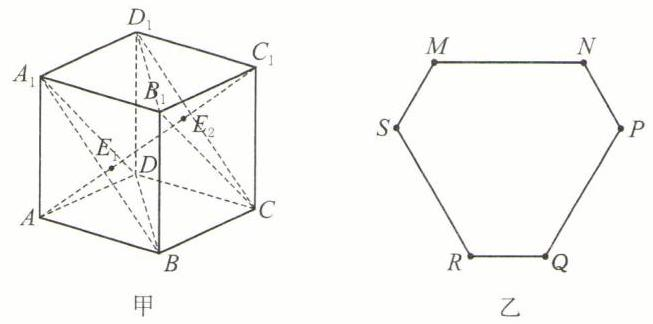
\includegraphics[width=0.5\textwidth]{bodyxb/src/bo_d20cdrf7aajc73bfmvhg_123_425_683_653_324_0.jpg}
        \end{center}
    \end{jieda} 
    \item \begin{enumerate}
        \item 在 ${{Rt}} \bigtriangleup  {ACB}$ 中,已知 $\angle {ACB} = {90}^{ \circ  },{AC} = {BC} = 1,{PA}\bot$ 平面 ${ABC}$ ,且 ${PA} = \sqrt{2}$ (如图),则 ${BP}$ 与平面 ${PAC}$ 所成的角等于\blkda{$\ang{30}$}
        \begin{center}
        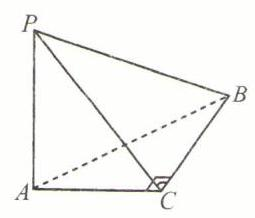
\includegraphics[width=0.2\textwidth]{bodyxb/src/bo_d20aucref24c73anc48g_148_454_647_255_218_0.jpg}
        \end{center}
        \begin{jieda}
            ${BC}$ 垂直于相交直线 ${AC}\text{ 、 }{AP}$ ,故 ${BC} \bot$ 平面 ${PAC}$ , $\therefore {BP}$ 与平面 ${PAC}$ 所成的角为 $\angle {BPC}$ (锐角). 不难求得 ${AB} = \sqrt{2},{BP} = 2,\therefore \sin \angle {BPC} = \dfrac{BC}{BP} = \dfrac{1}{2},\therefore \angle {BPC} = {30}^{ \circ  }$ 
        \end{jieda}
        \item 已知 ${AD}$ 是平面 $\alpha$ 的斜线, $D$ 为斜足, ${BD}$ 是 ${AD}$ 在 $\alpha$ 上的射影, ${DC}$ 在 $\alpha$ 内,且 $\angle {BDC} = \angle {ADB} = {45}^{ \circ  }$ (如图),则锐角 $\angle {ADC}$ 为\blkda{${60}^{ \circ  }$}
        \begin{center}
        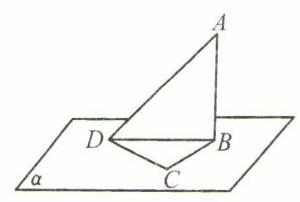
\includegraphics[width=0.2\textwidth]{bodyxb/src/bo_d20aucref24c73anc48g_148_967_661_300_202_0.jpg}
        \end{center}
        \begin{jieda}
            $cos\angle{ADC} = cos\angle{ADB} \cdot cos\angle{CDB}$
        \end{jieda}
        \item 已知斜线 ${AB}$ 与平面 $\alpha$ 所成角为 ${\theta }_{1},A \in  \alpha ,{AC} \subset  \alpha ,{AC}$ 与 ${AB}$ 在 $\alpha$ 上的射影 $A{B}_{1}$ 所成角为 ${\theta }_{2},{AC}$ 与 ${AB}$ 所成角为 $\theta$ ,则 $\cos \theta  =$ \blkda[2]{$\cos {\theta }_{1} \cdot  \cos {\theta }_{2}$}
    \end{enumerate}
    \item 在正方体 ${ABCD} - {A}_{1}{B}_{1}{C}_{1}{D}_{1}$ 中,求证:
    \begin{enumerate}
        \item 正方体对角线 $A{C}_{1} \bot$ 面对角线 ${B}_{1}C$
        \item $A{C}_{1} \bot$ 截面 $C{B}_{1}{D}_{1}$
    \end{enumerate}
    \begin{jieda}
        \begin{enumerate}
            \item 证明: ${AB} \bot$ 平面 $B{B}_{1}{C}_{1}C,\therefore B{C}_{1}$ 是 $A{C}_{1}$ 在 $B{B}_{1}{C}_{1}C$ 上的射影,由三垂线定理, ${B}_{1}C \bot  B{C}_{1} \Longrightarrow  {B}_{1}C \bot  A{C}_{1}$ ,证毕. (同理可证 $A{C}_{1} \bot  {D}_{1}C,A{C}_{1} \bot  {B}_{1}{D}_{1}$ ).
            \item 证明:由(1)可知: $A{C}_{1}$ 垂直于相交直线 ${B}_{1}C$ 和 ${B}_{1}{D}_{1},\therefore A{C}_{1} \bot$ 截面 $C{B}_{1}{D}_{1}$ ,证毕.
        \end{enumerate}
    \end{jieda}
    \item 已知 $H$ 为 $\bigtriangleup {ABC}$ 的垂心, ${PH} \bot$ 平面 ${ABC}$ ,且 $\angle {APB} = {90}^{ \circ  }$ (如图),求证: ${PC}\bot {PB}$
    
    \begin{center}
    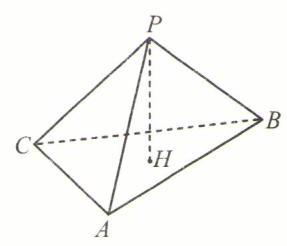
\includegraphics[width=0.2\textwidth]{bodyxb/src/bo_d20aucref24c73anc48g_148_1200_1176_287_246_0.jpg}
    \end{center}

    \begin{jieda}
        因为${PH} \bot$ 平面 ${ABC}$，所以$BP$在面$ABC$内的射影为$BH$，又因为$H$ 为 $\bigtriangleup {ABC}$ 的垂心, 所以$BH \bot AC$，故根据三垂线定理可知$BP \bot AC$，又因为$PB \bot AP$，$AP \cap AC = A$，所以$PB \bot $平面$PAC$，故$PC \bot PB$.
    \end{jieda}
    \item 
    \begin{enumerate}
        \item 在正方体 ${ABCD} - {A}_{1}{B}_{1}{C}_{1}{D}_{1}$ 中,已知 $M$ 为 $A{A}_{1}$ 的中点,点 $N$ 在 ${A}_{1}{B}_{1}$ 上且 ${A}_{1}N = \dfrac{1}{3}N{B}_{1}$ (如图),求证: ${MN}\bot {MC}$
        \begin{center}
        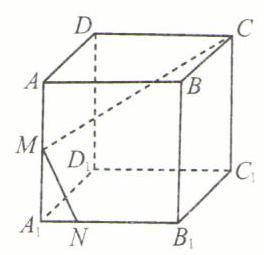
\includegraphics[width=0.2\textwidth]{bodyxb/src/bo_d20aucref24c73anc48g_148_351_1622_264_255_0.jpg}
        \end{center}
        \begin{jieda}
            先证 ${MN}\bot {BM}$ ,于是 ${BM}$ 是 ${MC}$ 在面 $A{A}_{1}{B}_{1}B$ 上的射影, $\therefore {MN}\bot {MC}$ . 注意, ${MN}\bot {BM}$ 是因为 $\bigtriangleup M{A}_{1}N \sim  \bigtriangleup {BAM},\therefore \angle {A}_{1}{MN} + \angle {AMB} = {90}^{ \circ  },\therefore \angle {BMN} = {90}^{ \circ  }$ .
        \end{jieda}
        \item 已知 ${PA}$ 是 $\bigtriangleup {ABC}$ 所在平面 $\alpha$ 的斜线,且 ${PA}\bot {BC},\angle {ACB} = {90}^{ \circ  }$ (如图),求证:点 $P$ 在平面 $\alpha$ 上的射影在直线 ${AC}$ 上
        \begin{center}
        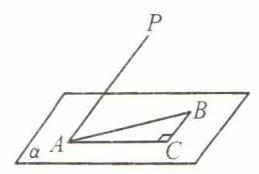
\includegraphics[width=0.2\textwidth]{bodyxb/src/bo_d20aucref24c73anc48g_148_739_1703_259_174_0.jpg}
        \end{center}
        \begin{jieda}
            证明:作 ${PO}\bot \alpha$ 于 $O$ ,则可证得 ${AO}\bot {BC}$ ,又 ${AC}\bot {BC}$ ,又 ${AO},{AC} \subset  \alpha$ , $\therefore O$ 在直线 ${AC}$ 上,证毕.
        \end{jieda}
        \item 在长方体 ${ABCD} - {A}_{1}{B}_{1}{C}_{1}{D}_{1}$ 中,已知 $E$ 在上底面 ${A}_{1}{B}_{1}{C}_{1}{D}_{1}$ 内, $\angle {A}_{1}{B}_{1}E = {60}^{ \circ  }$ , ${A}_{1}{B}_{1} = 2{B}_{1}E$ (如图),求证: ${AE} \bot  {B}_{1}E$
        \begin{center}
        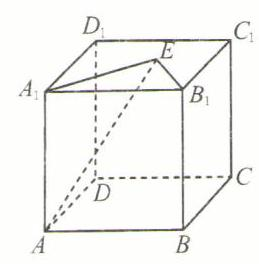
\includegraphics[width=0.2\textwidth]{bodyxb/src/bo_d20aucref24c73anc48g_148_1118_1612_259_264_0.jpg}
        \end{center}
        \begin{jieda}
            证明:先证 ${A}_{1}E\bot {B}_{1}E$ ,于是 ${A}_{1}E$ 是 ${AE}$ 在面 ${A}_{1}{B}_{1}{C}_{1}{D}_{1}$ 上的射影, $\therefore {AE}\bot {B}_{1}E$ . 注: ${A}_{1}E\bot {B}_{1}E$ 的证明如下: 设 ${B}_{1}E = x$ ,则 ${B}_{1}{A}_{1} = {2x}$ ,由余弦定理, $\cos \angle {A}_{1}{B}_{1}E = \dfrac{{x}^{2} + {\left( 2x\right) }^{2} - {A}_{1}{E}^{2}}{2 \cdot  x \cdot  {2x}} = {\cos }^{2}{60},\therefore {A}_{1}E = \sqrt{3}x$ ，$\therefore \angle {A}_{1}E{B}_{1} = {90}^{ \circ  }$ .
        \end{jieda}
    \end{enumerate}
    \item 已知矩形 ${ABCD}$ 的边长 ${AB} = 6{{cm}},{BC} = 4{{cm}}$ ,在 ${CD}$ 上截取 ${CE} =$  $4{{cm}}$ ,以 ${BE}$ 为棱将矩形折起,使 $\bigtriangleup B{C}^{\prime }E$ 的高 ${C}^{\prime }F \bot$ 平面 ${ABED}$ (如图), 求:
    
    \begin{center}
    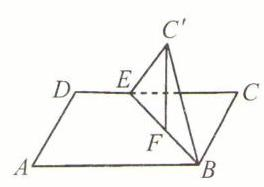
\includegraphics[width=0.2\textwidth]{bodyxb/src/bo_d20aucref24c73anc48g_149_1145_141_264_187_0.jpg}
    \end{center}
    \begin{enumerate}
        \item 点 ${C}^{\prime }$ 到平面 ${ABED}$ 的距离
        \item 点 ${C}^{\prime }$ 到边 ${AB}$ 的距离
        \item 点 ${C}^{\prime }$ 到 ${AD}$ 的距离
    \end{enumerate}
    \begin{jieda}
        \begin{enumerate}
            \item 作 ${FH}\bot {AB}$ 于 $H$ ,作 ${FG}\bot {AD}$ 于 $G$ ,则 ${C}^{\prime }H\bot {AB}$ , ${C}^{\prime }G\bot {AD}$ ,可算得 ${BE} = 4\sqrt{2}{{cm}}$ , ${HB} = 2{{cm}}$，$\therefore {C}^{\prime }$ 到面 ${ABED}$ 的距离为 ${C}^{\prime }F = 2\sqrt{2}{{cm}}$ .
            \item ${C}^{\prime }$ 到 ${AB}$ 的距离为 ${C}^{\prime }H = 2\sqrt{3}{{cm}}$ .
            \item ${C}^{\prime }$ 到 ${AD}$ 的距离为 ${C}^{\prime }G = 2\sqrt{6}{{cm}}$ .
        \end{enumerate}
    \end{jieda}
    \item \begin{enumerate}
        \item 在正方体 ${ABCD} - {A}_{1}{B}_{1}{C}_{1}{D}_{1}$ 中,求面对角线 ${A}_{1}B$ 与对角面 $B{B}_{1}{D}_{1}D$ 所成的角
        \begin{jieda}
            连接 ${A}_{1}{C}_{1}$ 与 ${B}_{1}{D}_{1}$ 交于点 $E$ ,连接 ${BE}.{A}_{1}{C}_{1} \bot  {B}_{1}{D}_{1},{A}_{1}{C}_{1} \bot  {B}_{1}B,\therefore {A}_{1}{C}_{1} \bot$ 平面 $B{B}_{1}{D}_{1}D,\therefore {A}_{1}B$ 与平面 $B{B}_{1}{D}_{1}D$ 所成的角是 $\angle {A}_{1}{BE}.\sin \angle {A}_{1}{BE} = \dfrac{{A}_{1}E}{{A}_{1}B} = \dfrac{\dfrac{\sqrt{2}}{2}{A}_{1}{B}_{1}}{\sqrt{2}{A}_{1}{B}_{1}} = \dfrac{1}{2},\therefore \angle {A}_{1}{BE} = {30}^{ \circ  }$ .
        \end{jieda}
        \item 在正四面体 ${ABCD}$ 中,已知 $M$ 是棱 ${AB}$ 的中点,求 ${CM}$ 与底面 ${BCD}$ 所成角的正弦值
        \begin{jieda}
            取 ${CD}$ 中点 $N$ ,连接 ${AN}$ , ${BN}$ ,则 ${CD} \bot$ 平面 ${ABN}$ . 在平面 ${ABN}$ 中,作 ${MP}\bot {BN}$ 于 $P,\because {MP} \bot  {BN},{MP} \bot  {CD},\therefore {MP} \bot$ 平面 ${BCD}$ ,即 $P$ 是 $M$ 在平面 ${BCD}$ 上的射影. 记 $\bigtriangleup {ABN}$ 中 ${BN}$ 边上的高为 $h$ ,则 ${MP} = \dfrac{1}{2}h = \dfrac{1}{2} \cdot  \dfrac{{AB} \cdot  {MN}}{BN}$ (面积法),得 ${MP} = \dfrac{\sqrt{6}}{6},\therefore \sin \angle {MCP} = \dfrac{MP}{MC} = \dfrac{\sqrt{2}}{3}$ . 
            
            \ps 先找到 ${AB}$ 在平面 ${BCD}$ 上的射影,此时再确定 ${AB}$ 上一点 $M$ 在该平面上的射影就相对容易了.
        \end{jieda}
        \item 从点 $P$ 出发的三条射线 ${PA},{PB},{PC}$ 两两都成 ${60}^{ \circ  }$ 角,求 ${PC}$ 与面 ${PAB}$ 所成角的余弦值
        \begin{jieda}
            在射线 ${PA}$ , ${PB}$ , ${PC}$ 上取 ${A}^{\prime }$ , ${B}^{\prime }$ , ${C}^{\prime }$ ,使 $P{A}^{\prime } = P{B}^{\prime } = P{C}^{\prime } = a$ ,可得正四面体 $P{A}^{\prime }{B}^{\prime }{C}^{\prime }$ ,问题转化为求棱 $P{C}^{\prime }$ 与底面 $P{A}^{\prime }{B}^{\prime }$ 所成角的余弦. ${C}^{\prime }$ 在 $P{A}^{\prime }{B}^{\prime }$ 上的射影是 $\bigtriangleup P{A}^{\prime }{B}^{\prime }$ 的中心,记为 $O$ ,则 $\cos \angle {C}^{\prime }{PO} = \dfrac{PO}{P{C}^{\prime }} = \dfrac{\dfrac{2}{3} \cdot  \dfrac{\sqrt{3}}{2}a}{a}$  $= \dfrac{\sqrt{3}}{3}$ .
        \end{jieda}
    \end{enumerate}
    \item 从平面 $\alpha$ 外一点 $P$ 向平面 $\alpha$ 引垂线 ${PO}$ 和斜线 ${PA},{PB}$ ,垂足为 $O$ ,斜足为 $A,B$ 
    \begin{enumerate}
        \item 若 ${PA}$ , ${PB}$ 和平面 $\alpha$ 所成角的差为 ${45}^{ \circ  }$ ,且在平面 $\alpha$ 上的射影长分别为 2 和 12,求 ${PO}$ 的长
        \begin{jieda}
            根据题意可知$\angle{PAO} = \angle{PBO} + \ang{45}$，$tan\angle{PAO} = \dfrac{PO}{2}, tan\angle{PBO} = \dfrac{PO}{12}$，故根据两角和的正切公式可知$\dfrac{PO}{2} = \dfrac{1+\dfrac{PO}{12}}{1-\dfrac{PO}{12}} = \dfrac{12+PO}{12-PO}$，解得$PO = 4$或$6$.
        \end{jieda}
        \item 若 $\angle {APB} = {60}^{ \circ  },{PA},{PB}$ 分别和 $\alpha$ 成 ${30}^{ \circ  },{45}^{ \circ  }$ 角,求 $\cos \angle {AOB}$ 的值
        \begin{jieda}
            设 ${OB} = a$ ,则 ${OP} = a$ , ${PB} = \sqrt{2}a$ , ${OA} = \sqrt{3}a$ , ${PA} = {2a}$ . 由余弦定理, $A{B}^{2} = P{A}^{2} + P{B}^{2} - 2 \cdot  {PA} \cdot  {PB} \cdot  \cos \angle {APB} = \left( {6 - 2\sqrt{2}}\right) {a}^{2},\cos \angle {AOB} = \dfrac{O{A}^{2} + O{B}^{2} - A{B}^{2}}{2 \cdot  {OA} \cdot  {OB}} = \dfrac{\sqrt{6} - \sqrt{3}}{3}\text{ . }$
        \end{jieda}
        \item 若 ${PA} : {PB} = 2 : 3,{PA},{PB}$ 与 $\alpha$ 所成角之比为 $2 : 1$ ,求 ${PB}$ 与 $\alpha$ 所成角的正弦值
        \begin{jieda}
            记 ${PB}$ 与 $\alpha$ 所成角为 $\theta  \in  \left( {0,\dfrac{\pi }{4}}\right)$ ,由题意, $\sin {2\theta } = \dfrac{PO}{PA}$ , $\sin \theta  = \dfrac{PO}{PB}$ , $\therefore \dfrac{\sin {2\theta }}{\sin \theta } = 2\cos \theta  = \dfrac{PB}{PA} = \dfrac{3}{2}$ , $\therefore \cos \theta  =$  $\dfrac{3}{4},\therefore \sin \theta  = \dfrac{\sqrt{7}}{4}$ .
        \end{jieda}
    \end{enumerate}
    \item 
    \begin{enumerate}
        \item 已知正方体 ${ABCD} - {A}_{1}{B}_{1}{C}_{1}{D}_{1}$ 中, $M$ 为 $A{A}_{1}$ 的中点, $P$ 为下底面 ${ABCD}$ 的中心, 求证: ${MP}\bot {B{C}_{1}}$
        \begin{jieda}
            先证 ${MP}//{A}_{1}C$ ,再证 ${A}_{1}C\bot B{C}_{1}$
        \end{jieda}
        \item 已知 ${{Rt}}\bigtriangleup {ABC}$ 的斜边 ${BC}$ 在平面 $\alpha$ 内,两直角边 ${AB},{AC}$ 与 $\alpha$ 都斜交, $A$ 在 $\alpha$ 上的射影是 ${A}^{\prime }\left( {A}^{\prime }\right.$ 不在 ${BC}$ 上),求证: $\angle B{A}^{\prime }C$ 是钝角
        \begin{jieda}
            $cos\angle{B{A}^{\prime }C} = \dfrac{A'B^2+A'C^2-BC^2}{2A'B \cdot A'C}$
    
            根据勾股定理可知$AB^2+AC^2 = BC^2$，又因为$AC > A'C, BC > B'C$，因此$cos\angle{B{A}^{\prime }C} < 0$
        \end{jieda}
        \item 已知 ${PA},{PB},{PC}$ 与平面 $\alpha$ 所成的角分别为 ${60}^{ \circ  },{45}^{ \circ  },{30}^{ \circ  },{PO}\bot$ 平面 $\alpha ,O$ 为垂足,又斜足 $A,B,C$ 三点在同一直线上,且 ${AB} = {BC} = {10}{{cm}}$ (如图),求 ${PO}$ 的长
        \begin{center}
        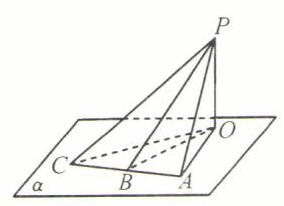
\includegraphics[width=0.2\textwidth]{bodyxb/src/bo_d20aucref24c73anc48g_149_382_1340_284_206_0.jpg}
        \end{center}
        \begin{jieda}
            根据题意可知$AO = \dfrac{\sqrt{3}}{3}PO, BO = PO, CO = \sqrt{3}PO$，根据余弦定理有$\dfrac{BO^2+BA^2-AO^2}{2BA\cdot BO} = -\dfrac{BO^2+BC^2-CO^2}{2BC \cdot BO}$，代入可得$PO = 5\sqrt{6} cm$
        \end{jieda}
        \item 已知 ${OA},{OB},{OC}$ 分别是平面 $\alpha$ 内过点 $O$ 的三条射线,射线 ${PO}$ 交 $\alpha$ 于点 $O$ (如图). \ding{172}若 ${PO}$ 和 $\alpha$ 斜交,且 $\angle {POA} = \angle {POB}$ ,求证: ${PO}$ 在 $\alpha$ 上的射影是 $\angle {AOB}$ 的平分线或它的反向延长线，\ding{173}若 $\angle {POA} = \angle {POB} = \angle {POC}$ ,求证: ${PO}\bot \alpha$ 
        \begin{center}
        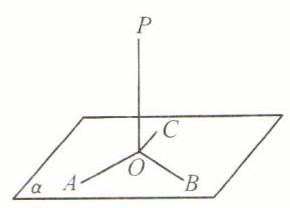
\includegraphics[width=0.2\textwidth]{bodyxb/src/bo_d20aucref24c73anc48g_149_927_1333_290_208_0.jpg}
        \end{center}
        \begin{jieda}
            记点 $P$ 在平面 $\alpha$ 上的射影为 $Q$ ,连接 ${OQ}$ .
            
            \ding{172}由$\cos \angle {POA} = \cos \angle {AOQ} \cdot  \cos \angle {POQ},\cos \angle {POB} = \cos \angle {BOQ} \cdot  \cos \angle {POQ}$ .
            
            $\because {PO}$ 和 $\alpha$ 斜交, $\therefore \angle {POA},\angle {POB},\angle {POQ}$ 均不为 $\dfrac{\pi }{2}$ (余弦值不为 0), $\therefore \cos \angle {AOQ} = \cos \angle {BOQ} \Longrightarrow$  $\angle {AOQ} = \angle {BOQ}$ ,证毕.

            \ding{173}若 ${PO}$ 与 $\alpha$ 斜交,则作 ${PH}\bot \alpha$ 于 $H$ . 由\ding{172}知: ${OH}$ 既是 $\angle {AOB}$ ,也是 $\angle {BOC}$ 的平分线,这要求 ${OC}$ 与 ${OA}$ 或 ${OB}$ 重合,矛盾,故 ${PO}\bot \alpha$ ,证毕.
        \end{jieda}
    \end{enumerate}
    \item $P$ 为 ${{Rt}} \bigtriangleup  {ABC}$ 所在平面 $\alpha$ 外一点, $\angle {ACB} = {90}^{ \circ  }$ (如图).
    
    \begin{center}
    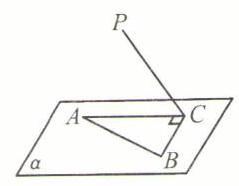
\includegraphics[width=0.2\textwidth]{bodyxb/src/bo_d20aucref24c73anc48g_149_1177_1793_239_186_0.jpg}
    \end{center}

    \begin{enumerate}
        \item 若 ${PC} = a,\angle {PCA} = \angle {PCB} = {60}^{ \circ  }$ ,求 $P$ 到 $\alpha$ 的距离及 ${PC}$ 和 $\alpha$ 所成的角
        \item 若 ${PC} = {24},P$ 到 ${AC},{BC}$ 的距离都是 $6\sqrt{10}$ ,求 $P$ 到 $\alpha$ 的距离及 ${PC}$ 和 $\alpha$ 所成的角
        \item 若 ${PA} = {PB} = {PC},{AC} = {18},P$ 到 $\alpha$ 的距离为 40,求 $P$ 到 ${BC}$ 的距离.
    \end{enumerate}
    \begin{jieda}
        \begin{enumerate}
            \item 记点 $P$ 在平面 $\alpha$ 上的射影是点 $Q$ ,连接 ${CQ}$.
            \begin{enumerate}
                \item $\angle {PCA} = \angle {PCB}$ 且为锐角 $\Longrightarrow  {CQ}$ 是 $\angle {ACB}$ 的角平分线, $\angle {ACQ} = {45}^{ \circ  },\cos \angle {PCA} = \cos \angle {PCQ} \cdot  \cos \angle {ACQ}$ ,解得 $\angle {PCQ} = {45}^{ \circ  }$ ,即为 ${PC}$ 和 $\alpha$ 所成的角. $P$ 到 $\alpha$ 的距离 $= {PC} \cdot  \sin \angle {PCQ} = \dfrac{\sqrt{2}}{2}a$ .
                \item 记 ${PD}\bot {AC}$ 于 $D,{PE}\bot {BC}$ 于 $E$ ,由题意可证 $\bigtriangleup  {PCD} \cong   \bigtriangleup  {PCE},\therefore \angle {PCD} = \angle {PCE} = \theta ,\sin \theta  = \dfrac{6\sqrt{10}}{24} = \dfrac{\sqrt{10}}{4}$ , $\therefore \cos \theta  =  \pm  \dfrac{\sqrt{6}}{4},\cos \theta  = \cos \angle {PCQ} \cdot  \cos \angle {ACQ}$ . 当 $\cos \theta  > 0\left( { < 0}\right)$ 时, ${CQ}$ 是 $\angle {ACB}$ 的角平分线 (反向延长线), $\therefore \cos \angle {PCQ} = \dfrac{\sqrt{3}}{2},P$ 到 $\alpha$ 的距离为 ${PC} \cdot  \sin \angle {PCQ} = {12};{PC}$ 和 $\alpha$ 所成的角为 $\angle {PCQ} = {30}^{ \circ  }$ .
                \item 由题意,点 $Q$ 是 ${{Rt}} \bigtriangleup  {ACB}$ 的外心,也即边 ${AB}$ 的中点. 取边 ${BC}$ 的中点 $R$ ,连接 ${QR}$ 、 ${PR}$ . ${QR} = \dfrac{1}{2}{AC} = 9$ ,由三垂线定理, ${QR} \bot  {BC} \Longrightarrow  {PR} \bot  {BC},{PR} = \sqrt{P{Q}^{2} + Q{R}^{2}} = \sqrt{{40}^{2} + {9}^{2}} = {41}$ ,即为所求.
            \end{enumerate}
        \end{enumerate}
    \end{jieda}
    \item 在正方体 ${ABCD} - {A}_{1}{B}_{1}{C}_{1}{D}_{1}$ 中, $E,F$ 分别是棱 ${BC},{A}_{1}{D}_{1}$ 的中点 (如图),求棱 ${AD}$ 与平面 ${B}_{1}{EDF}$ 所成角的余弦值.
    
    \begin{center}
    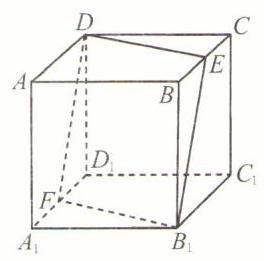
\includegraphics[width=0.2\textwidth]{bodyxb/src/bo_d20aucref24c73anc48g_150_525_257_264_261_0.jpg}
    \end{center}
    \begin{jieda}
        易证 $\bigtriangleup D{D}_{1}F \cong  \bigtriangleup {DCE},\therefore \angle {FD}{D}_{1} = \angle {EDC},\therefore \angle {ADF} = \angle {ADE}$ (且为锐角)，故可知射线 ${DA}$ 在平面 ${B}_{1}{EDF}$ 上的射影为 $\angle {FDE}$ 的角平分线,即射线 $D{B}_{1}$ . 连接 ${B}_{1}D\text{ 、 }{B}_{1}A,\operatorname{Rt} \bigtriangleup  {DA}{B}_{1}$ 中, $\angle {DA}{B}_{1} = {90}^{ \circ  }$ , $\cos \angle {AD}{B}_{1} = \dfrac{DA}{D{B}_{1}} = \dfrac{\sqrt{3}}{3}$ 即为所求. 
    \end{jieda}

    \item 线段 ${AB}$ 两端在平面 $\alpha$ 同侧,斜线 ${AM},{BN}$ 与 $\alpha$ 分别成 ${30}^{ \circ  },{60}^{ \circ  }$ 角 $\left( {M,N\text{ 为斜足 }}\right)$ ,且 ${AM} \bot  {AB},{BN} \bot  {AB},{AM} = 6,{BN} = 2\sqrt{3},{AB} = 6$ (如图).
    \begin{enumerate*}
        \item 求证: ${AB}//\alpha$
        \item 求 ${MN}$ 的长.
    \end{enumerate*}
    \begin{center}
    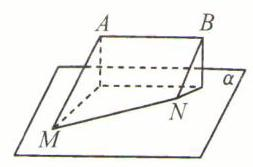
\includegraphics[width=0.2\textwidth]{bodyxb/src/bo_d20aucref24c73anc48g_150_915_350_253_167_0.jpg}
    \end{center}
    \begin{jieda}
        记 $A,B$ 在平面 $\alpha$ 上的射影为 $C,D$ .
        \begin{enumerate}
            \item 证明: $\because {AC}\bot \alpha ,{BD}\bot \alpha$ , $\therefore {AC}//{BD}$ . 又 ${AC} = {AM} \cdot  \sin {30}^{ \circ  } = 3,{BD} = {BN} \cdot  \sin {60}^{ \circ  } = 3,\therefore {AC}\bot {BD}$，$\therefore$ 四边形 ${ABCD}$ 是平行四边形, $\therefore {AB}//{CD},{CD} \subset  \alpha ,\therefore {AB}//\alpha$ ,证毕.
            \item $\because {AB}\bot {AM},{AB}//{CD},\therefore {CD}\bot {AM},{AM}$ 在 $\alpha$ 上的射影是 ${CM}$ ,由三垂线定理, ${CD}\bot {CM}$ . 同理, ${CD}\bot {DN}$ . 当 $M$ , $N$ 在 ${CD}$ 两侧时, ${MN} = \sqrt{C{D}^{2} + {\left( CM + DN\right) }^{2}} = 2\sqrt{21}$ ; 当 $M,N$ 在 ${CD}$ 同侧时, ${MN} = \sqrt{C{D}^{2} + {\left( CM - DN\right) }^{2}} = 4\sqrt{3}$ .
        \end{enumerate}
    \end{jieda}
    \item \begin{enumerate}
        \item 若直角 $\angle {ABC}$ 的一边 ${BC}$ 平行于平面 $\alpha$ ,另一边 ${AB}$ 和平面 $\alpha$ 斜交 (如图),求证: $\angle {ABC}$ 在平面 $\alpha$ 上的射影仍是直角
        \begin{center}
        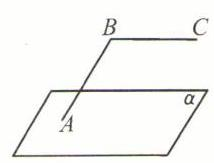
\includegraphics[width=0.2\textwidth]{bodyxb/src/bo_d20aucref24c73anc48g_150_1287_723_214_163_0.jpg}
        \end{center}
        \begin{jieda}
            作 ${BD}\bot \alpha ,{CE}\bot \alpha ,D,E$ 为垂足,连接 ${DE},{DA},{BD}//{CE}$ ,它们确定的平面记为 $\beta$ .
            
            ${BC} \subset  \beta ,\beta  \cap  \alpha  = {DE},{BC}//\alpha ,\therefore {BC}//{DE},{BC}\bot {BA} \Longrightarrow  {DE}\bot {BA}$ ,由三垂线定理, ${DE}\bot {DA}$ ,即 $\angle {ABC}$ 在平面 $\alpha$ 上的射影 $\angle {ADE} = {90}^{ \circ  }$ ,证毕.
        \end{jieda}
        \item 直角 $\angle {ABC}$ 的一条边 ${AB}$ 和平面 $\alpha$ 斜交,另一边 ${BC}$ 不在平面 $\alpha$ 内,若 $\angle {ABC}$ 在 $\alpha$ 上的射影仍是直角,求证: ${BC}//\alpha$ .
        \begin{jieda}
            作 ${BD}\bot \alpha ,{CE}\bot \alpha ,D,E$ 为垂足,连接 ${DE},{DA},{BD}//{CE}$ ,它们确定的平面记为 $\beta$ .
            
            由勾股定理, $A{B}^{2} + B{C}^{2} = A{C}^{2}$ ,代入 $A{B}^{2} = A{D}^{2} + B{D}^{2}$ , $A{C}^{2} = A{E}^{2} + E{C}^{2} = A{D}^{2} + D{E}^{2} + E{C}^{2}$ ,整理得 $B{D}^{2} + B{C}^{2} = E{C}^{2} + D{E}^{2} = C{D}^{2}$ , $\therefore$ 在 $\beta$ 内, ${BC}\bot {BD}$ ,又 ${DE}\bot {BD}$ , $\therefore {BC}//{DE}$ , $\therefore {BC}//\alpha$ ,证毕.
        \end{jieda}
    \end{enumerate}

\end{enumerate}
\section*{四、平面与平面的位置关系}

\subsection*{(一) 两个平面平行}

\subsubsection*{【典型题型和解题技巧】}

1. 两个平面平行的证明.

(1)利用面面平行的定义.

定义 如果两个平面没有公共点, 就称这两个平面平行.

(2)利用面面平行的判定定理.

\textbf{定理} 如果一个平面上有两条相交直线都平行于另一个平面, 那么这两个平面互相平行.

\textbf{例 1} 如果两条异面直线都和两个平面平行, 那么这两个平面互相平行.

已知: $l,m$ 是两条异面直线, $l//$ 平面 $\alpha ,l//$ 平面 $\beta ,m//\alpha ,m//\beta$ ,求证: $\alpha //\beta$ .

\textbf{证明} 

过 $l$ 作平面 $\gamma$ ,使 $\gamma$ 和平面 $\alpha ,\beta$ 分别交于 ${l}_{1},{l}_{2}$ ; 过 $m$ 作平面 $\varphi$ , 使 $\varphi$ 和平面 $\alpha ,\beta$ 分别交于 ${m}_{1},{m}_{2}$ (如图).

\begin{center}
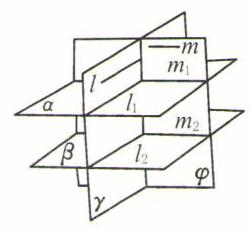
\includegraphics[width=0.2\textwidth]{bodyxb/src/bo_d20aucref24c73anc48g_150_1253_1782_251_229_0.jpg}
\end{center}

$\because l//\alpha ,\therefore l//{l}_{1}$，又 $\because l//\beta ,\therefore l//{l}_{2}.\therefore {l}_{1}//{l}_{2}$，而 ${l}_{1}$ 不在平面 $\beta$ 上, ${l}_{2} \subset  \beta ,\therefore {l}_{1}//\beta$ .

同理 ${m}_{1}//\beta$，显然, ${l}_{1},{m}_{1}$ 相交,故 $\alpha //\beta$ .

2. 利用面面平行的性质解题.

(1)利用面面平行的定义,如果两个平面平行,那么这两个平面没有公共点. 可记为

平面 $\alpha //$ 平面 $\beta  \Longrightarrow  \alpha  \cap  \beta  = \varnothing$ .

(2)利用面面平行的性质定理.

\textbf{定理} 如果两个平行平面同时和第三个平面相交, 那么它们的交线互相平行.

定理可概括为:“若面面平行,则交线平行”,

$\left. \begin{array}{l} \text{ 平面 }\alpha //\text{ 平面 }\beta , \\  \text{ 平面 }\alpha  \cap  \text{ 平面 }\gamma  = \text{ 直线 }a, \\  \text{ 平面 }\beta  \cap  \text{ 平面 }\gamma  = \text{ 直线 }b, \end{array}\right\}   \Longrightarrow  a//b$ .

\textbf{例 2} 已知两条异面线段 ${AB},{CD}$ 的端点 $A,C$ 和 $B,D$ 分别在两个平行平面 $\alpha ,\beta$ 内, $P,Q$ 分别是 ${AB},{CD}$ 的中点 (如图),求证: ${PQ}//\alpha$ , ${PQ}//\beta$ .

\begin{center}
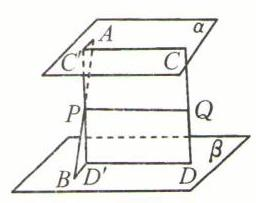
\includegraphics[width=0.2\textwidth]{bodyxb/src/bo_d20aucref24c73anc48g_151_1149_709_256_203_0.jpg}
\end{center}

\textbf{证明} 

在由 ${PQ},{CD}$ 所确定的平面上,过点 $P$ 作 ${CD}$ 的平行线 ${C}^{\prime }{D}^{\prime }$ , 与平面 $\alpha ,\beta$ 分别相交于点 ${C}^{\prime },{D}^{\prime }.C{C}^{\prime }$ 和 $D{D}^{\prime }$ 分别是平面 ${CD}{D}^{\prime }{C}^{\prime }$ 与两个平行平面的交线,故 $C{C}^{\prime }//D{D}^{\prime }$ .

$\therefore$ 四边形 ${CD}{D}^{\prime }{C}^{\prime }$ 是平行四边形.

显然, ${AB}$ , ${C}^{\prime }{D}^{\prime }$ 相交,平面 $A{C}^{\prime }B{D}^{\prime }$ 和 $\alpha$ , $\beta$ 分别交于 $A{C}^{\prime }$ , $B{D}^{\prime }$ ,由 $\alpha //\beta$ 知, $A{C}^{\prime }//B{D}^{\prime }$ . 又 $P$ 是 ${AB}$ 的中点，$\therefore P$ 也是 ${C}^{\prime }{D}^{\prime }$ 的中点,于是 ${C}^{\prime }P\overset{//}{ = }{CQ}$ ,

$\therefore$ 四边形 ${CQP}{C}^{\prime }$ 是平行四边形，由 ${PQ}$ 不在平面 $\alpha$ 上, $C{C}^{\prime } \subset  \alpha ,{PQ}//C{C}^{\prime }$ ,可得 ${PQ}//\alpha$ .

同理可得 ${PQ}//\beta$ .

(3)利用面面平行性质定理的推论.

推论 若一条直线垂直于两个平行平面中的一个平面,则它也垂直于另一个平面.

\subsubsection*{【训练题】}

\begin{center}  \textbf{(A)} \end{center}
\begin{enumerate}
    \item 已知 $a,b$ 是异面直线,且 $a\bot$ 平面 $\alpha ,b\bot$ 平面 $\beta$ ,则 $\alpha ,\beta$ 的位置关系是\dotfill{(\kh{A})}
    \xx{相交}{重合}{平行}{不能确定}
    \begin{jieda}
        两平面的关系仅有相交、重合、平行 3 种,若平面 $\alpha ,\beta$ 重合,则直线 $a$ 与 $b$ 重合或平行; 若平面 $\alpha ,\beta$ 平行,则直线 $a \bot$ 平面 $\alpha  \Longrightarrow$ 直线 $a \bot$ 平面 $\beta$ ,又 $b \bot$ 平面 $\beta$ ,故 $a$ 与 $b$ 重合或平行. 由题意, $a$ 与 $b$ 异面,因此平面 $\alpha ,\beta$ 必相交.
    \end{jieda}
    
    \item 有下列四个命题:\ding{172}分别在两个平行平面上的两条直线都平行；\ding{173}若两个平面平行,则其中一个平面上的直线必平行于另一个平面; \ding{174} 如果一个平面上的两条直线平行于另一个平面, 那么这两个平面平行; \ding{175}如果一个平面上的任何一条直线都平行于另一个平面, 那么这两个平面平行. 其中正确的个数是\dotfill{(\kh{B})}
    \xx{1}{2}{3}{4}
    \begin{jieda}
        \ding{172}错误,未考虑异面的可能性. \ding{173}正确,简证如下: $l \subset  \alpha ,\alpha  \cap  \beta  = \varnothing ,\therefore l \cap  \beta  = \varnothing$ ,即 $l//\beta$ ,证毕. \ding{174}错误,若这两条直线互相平行, 则这两个平面可能相交. \ding{175}正确, 取其中两条相交直线, 根据面面平行的判定定理, 可知这两个平面平行.
    \end{jieda}
    
    \item 下列命题不正确的是\dotfill{(\kh{C})}
    \xx{垂直于同一条直线的两个平面平行}{垂直于同一个平面的两条直线互相平行}{若一个平面上有无数条直线都平行于另一个平面, 则这两个平面互相平行}{若两个平行平面分别和第三个平面相交, 则它们的交线互相平行}
    \begin{jieda}
        选项 (C) 中,需注意 “无数条直线” 与 “任意直线” 的区别,一个反例是: 在正方体 ${ABCD} - {A}^{\prime }{B}^{\prime }{C}^{\prime }{D}^{\prime }$ 中,平面 ${AB}{B}^{\prime }{A}^{\prime }$ 内与 ${AB}$ 平行的直线都与平面 ${ABCD}$ 平行,但平面 ${AB}{B}^{\prime }{A}^{\prime } \cap$ 平面 ${ABCD} = {AB}$ .
    \end{jieda}

    \item 下列命题正确的是\dotfill{(\kh{A})}
    \xx{若平面 $\alpha$ 与平面 $\beta$ 相交但不垂直,则 $\alpha$ 内任意一条直线 $l$ 与 $\beta$ 都不垂直}{过平面 $\alpha$ 的一条斜线的平面 $\beta$ 与 $\alpha$ 一定不垂直}{若 ${l}_{1}$ 与 ${l}_{2}$ 是异面直线,则过 ${l}_{1}$ 一定能作一平面与 ${l}_{2}$ 垂直}{同时垂直于平面 $\alpha$ 的两个平面互相平行}
    \begin{jieda}
        选项 (A) 正确,反证法即可证明. 选项 (B) 错误,反例:在正方体 ${ABCD} - {A}^{\prime }{B}^{\prime }{C}^{\prime }{D}^{\prime }$ 中,取 $\alpha  =$ 平面 ${ABCD}$ 及其斜线 $A{B}^{\prime },\beta  =$ 平面 ${AB}{B}^{\prime }{A}^{\prime }$ . 选项 (C) 错误,参考本章第 68 题. 选项 (D) 错误,反例: 在正方体中,取 $\alpha$ 为底面,两个平面为两个相交侧面.
    \end{jieda}

    \item 有下列四个命题:\ding{172}若直线 $a//$ 直线 $b$ ,则 $a$ 和 $b$ 与平面 $\alpha$ 所成的角相等；\ding{173}若直线 $a$ 和 $b$ 与平面 $\alpha$ 所成的角相等,则 $a//b$ ; \ding{174}若 $\alpha //\beta$ ,则直线 $a$ 与平面 $\alpha$ ,平面 $\beta$ 所成的角相等; \ding{175}若平面 $\alpha$ ,平面 $\beta$ 都与直线 $a$ 平行,则 $\alpha //\beta$ . 其中正确的是\dotfill{(\kh{A})}
    \xx{\ding{172}和\ding{174}}{\ding{173}, \ding{174}和\ding{175}}{\ding{172},\ding{173}和\ding{174}}{都正确}
    \begin{jieda}
        \ding{172}正确,简证如下: 若 $a\bot a$ ,则结论显然成立; 若 $a$ 是 $a$ 的斜线,记直线 $a,b$ 和平面 $a$ 交于点 $A,B$ ,在直线 $a,b$ 上取点 $M,N$ ,使得 ${AM} = {BN}$ ,点 $M,N$ 在 $\alpha$ 上的射影是点 ${M}^{\prime },{N}^{\prime }$ ,易证 ${{Rt}}\bigtriangleup {MA}{M}^{\prime } \cong  {{Rt}}\bigtriangleup {NB}{N}^{\prime }$ ,故直线 $a,b$ 和平面 $\alpha$ 所成的角 $\angle {MA}{M}^{\prime } = \angle {NB}{N}^{\prime }$ ,证毕. \ding{173}错误,也可能相交或异面,例如在正方体 ${ABCD} - {A}^{\prime }{B}^{\prime }{C}^{\prime }{D}^{\prime }$ 中,取 $\alpha  =$ 平面 ${ABCD},a = A{B}^{\prime }$ ,当 $b = {A}^{\prime }B$ 时 $a,b$ 相交; 当 $b = {D}^{\prime }C$ 时 $a,b$ 异面. \ding{174}正确,简证如下: 若 $a\bot \alpha$ ,则结论显然成立; 若 $a$ 是 $\alpha$ 的斜线,记直线 $a$ 和平面 $\alpha ,\beta$ 交于点 $A,B$ ,在直线 $a$ 上取点 $M$ (异于 $A,B$ ),过 $M$ 作 $l \bot$ 平面 $\alpha$ (垂足为 ${A}^{\prime }$ ),则 $l \bot$ 平面 $\beta$ (垂足为 ${B}^{\prime }$ ). 易证 ${{Rt}}\bigtriangleup {MA}{A}^{\prime } \sim  {{Rt}}\bigtriangleup {MB}{B}^{\prime }$ ,故直线 $a$ 和平面 $\alpha ,\beta$ 所成的角 $\angle {MA}{A}^{\prime } = \angle {MB}{B}^{\prime }$ ,证毕. \ding{175}错误,也可能相交,例如在正方体 ${ABCD} - {A}^{\prime }{B}^{\prime }{C}^{\prime }{D}^{\prime }$ 中,取 $\alpha  =$ 平面 ${ABCD},\beta  =$ 平面 ${AB}{B}^{\prime }{A}^{\prime }$ ,直线 $\alpha  = {C}^{\prime }{D}^{\prime }$ .
    \end{jieda}
    \item 在正方体 ${ABCD} - {A}_{1}{B}_{1}{C}_{1}{D}_{1}$ 中,已知 $P,Q$ 分别是棱 $A{A}_{1},C{C}_{1}$ 的中点,则过点 $B,P,Q$ 的截面是\dotfill{(\kh{B})}
    \xx{邻边不等的平行四边形}{菱形但不是正方形}{邻边不等的矩形}{正方形}
    \begin{jieda}
        连接 ${D}_{1}P,{D}_{1}Q$ . 第 1 步: 证 ${D}_{1} \in$ 平面 ${PBQ}$ . 不难证明 $\bigtriangleup P{D}_{1}{A}_{1} \cong  \bigtriangleup {QBC},\therefore \angle P{D}_{1}{A}_{1} = \angle {QBC}$ . 设过点 ${D}_{1},P,B$ 的平面 $\alpha$ 与平面 ${BC}{C}_{1}{B}_{1}$ 的交线是 $B{Q}^{\prime },\because$ 平面 ${AD}{D}_{1}{A}_{1}//$ 平面 ${BC}{C}_{1}{B}_{1},\alpha  \cap  {AD}{D}_{1}{A}_{1} = {D}_{1}P,\alpha  \cap$  ${BC}{C}_{1}{B}_{1} = B{Q}^{\prime },\therefore {D}_{1}P//B{Q}^{\prime }$ ,又 ${D}_{1}{A}_{1}//{BC},\therefore \angle P{D}_{1}{A}_{1} = \angle {Q}^{\prime }{BC},\therefore {BQ}$ 与 $B{Q}^{\prime }$ 重合, $\therefore {D}_{1} \in$ 平面 ${PBQ}$ , $\therefore$ 截面即为四边形 ${D}_{1}{PBQ}$ . 第 2 步,确定四边形 ${D}_{1}{PBQ}$ 的形状. 我们已经证明 ${D}_{1}P//{QB}$ ,同理 ${PB}//{D}_{1}Q$ , 因此四边形 ${D}_{1}{PBQ}$ 是平行四边形. 记正方体棱长为 $a$ ,则 ${BP} = {BQ} = \dfrac{\sqrt{5}}{2}a,{PQ} = {AC} = \sqrt{2}a,\therefore \angle {PBQ} \neq  {90}^{ \circ  }$，$\therefore$ 四边形 ${D}_{1}{PBQ}$ 是菱形但不是正方形.
    \end{jieda}
    \item \begin{enumerate}
        \item 已知两平行平面 $\alpha ,\beta$ 间的距离为 2,点 $A \in  \alpha ,B \in  \beta$ ,且 ${AB}$ 的长为 4
        \begin{dingautolist}{172}
            \item 直线 ${AB}$ 与 $\alpha ,\beta$ 所成的角等于\blkda{${30}^{ \circ  }$}
            \item 若 $A$ 为 $\alpha$ 内的定点, $B$ 为 $\beta$ 内的动点,则 $B$ 点运动所形成的图形是\blkda[8]{以 $A$ 在 $\beta$ 上的射影为圆心,以 $2\sqrt{3}$ 为半径的圆}
        \end{dingautolist}
        \item 已知平面 $\alpha //$ 平面 $\beta$ ,点 $A,B \in  \alpha$ ,点 $C,D \in  \beta$ . 若 ${AC} = {70},{BD} = {37}$ ,且 ${BD}$ 在 $\beta$ 上的射影长为 12 ,则 ${AC}$ 与 $\beta$ 所成角为\blkda{$\ang{30}$}
        \begin{jieda}
            先算出两平面间距离为$\sqrt{37 \times 37-12\times 12} = 35$，故可知${AC}$ 与 $\beta$ 所成角为$\ang{30}$
        \end{jieda}
        \item 已知平面 $\alpha //$ 平面 $\beta ,{AC},{BD}$ 为夹在 $\alpha ,\beta$ 间的两斜线段 $\left( {A,B \in  \alpha ,C,D \in  \beta }\right)$ ,且 ${AC}$  $= {37},{BD} = {125},{AC}$ 在 $\beta$ 上的射影长为 12 ,则 ${BD}$ 在 $\beta$ 上的射影长为\blkda{120}
        \begin{jieda}
            先算出两平面间距离为$\sqrt{37 \times 37-12\times 12} = 35$，故可知${BD}$ 在 $\beta$ 上的射影长为120        
        \end{jieda}
    \end{enumerate}
    \item 在正方体 ${ABCD} - {A}_{1}{B}_{1}{C}_{1}{D}_{1}$ 中,已知 $E,F$ 分别为棱 $B{B}_{1},{B}_{1}{C}_{1}$ 的中点 (如图),则过 $A$ , $E,F$ 的截面的形状是\blkda{等腰梯形}.
    
    \begin{center}
    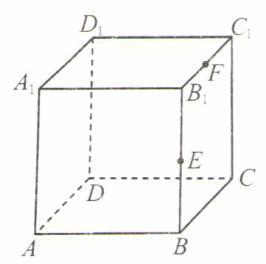
\includegraphics[width=0.15\textwidth]{bodyxb/src/bo_d20aucref24c73anc48g_152_520_1744_266_264_0.jpg}
    \end{center}
    \begin{jieda}
        ${EF}//B{C}_{1},B{C}_{1}//A{D}_{1},\therefore {EF}//A{D}_{1},\therefore A,E,F,{D}_{1}$ 四点共面,四边形 ${AEF}{D}_{1}$ 即为所求截面. 四边形 ${AEF}{D}_{1}$ 中, ${EF}//A{D}_{1},F{D}_{1}$ 与 ${EA}$ 不平行 (否则 $F{D}_{1}//{EA},{C}_{1}{D}_{1}//{AB} \Longrightarrow$ 平面 ${A}_{1}{B}_{1}{C}_{1}{D}_{1}//$ 平面 ${AB}{B}_{1}{A}_{1}$ ,矛盾), $\bigtriangleup F{C}_{1}{D}_{1} \cong  \bigtriangleup {EBA} \Longrightarrow  F{D}_{1} = {EA}$ ,因此截面的形状是等腰梯形 ${AEF}{D}_{1}$ .
    \end{jieda}
    \item \begin{enumerate}
        \item 已知: $a,b$ 是两条异面直线, $\alpha ,\beta$ 是两个不同平面,且 $a//\alpha ,a//\beta ,b//\alpha ,b//\beta$ ,求证: $\alpha // \beta$
        \begin{jieda}
            过$a$上一点$A$作$b$的平行线$b'$，过$a$的平面$\gamma_1$交$\alpha$和$\beta$于$a_1, a_2$，根据线面平行的性质定理可知$a // a_1, a // a_2$，故$a_1 // a_2$，因此$a_1 // \beta$，同理过$b'$的平面$\gamma_2$交$\alpha$和$\beta$于$b_1, b_2$，同理可证$b_1 // \beta$，易知$a_1$与$b_1$相交，所以根据面面平行判定定理可知$\alpha // \beta$
        \end{jieda}
        \item 在正方体 ${ABCD} - {A}_{1}{B}_{1}{C}_{1}{D}_{1}$ 中, $E$ , $F$ , $G$ 分别为 ${B}_{1}{C}_{1}$ , ${A}_{1}{D}_{1}$ , ${A}_{1}{B}_{1}$ 的中点(如图). 求证: 平面 ${EBD}//$ 平面 ${FGA}$
        \begin{center}
        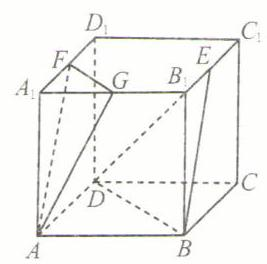
\includegraphics[width=0.2\textwidth]{bodyxb/src/bo_d20aucref24c73anc48g_152_908_1740_267_264_0.jpg}
        \end{center}
        \begin{jieda}
            易知$FG // BD$，因此$FG // $平面 ${EBD}$

            取$BD$中点$O$，连接$EO$，易知$AO$和$GE$平行且相等，因此$AOEG$为平行四边形，因此$AG // EO$，所以$AG //$平面 ${EBD}$

            故根据面面平行判定定理可知平面 ${EBD}//$ 平面 ${FGA}$
        \end{jieda}
    \end{enumerate}
    \item 已知平面 $\alpha //$ 平面 $\beta ,O$ 为 $\alpha ,\beta$ 外一点,三条射线 ${OA},{OB},{OC}$ 分别交 $\alpha$ 于点 ${A}_{1},{B}_{1},{C}_{1}$ ,交 $\beta$ 于点 $A,B,C$ (如图).
    
    \begin{center}
    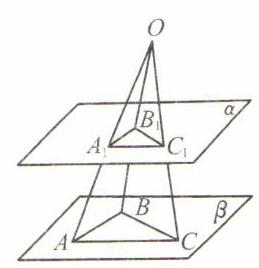
\includegraphics[width=0.2\textwidth]{bodyxb/src/bo_d20aucref24c73anc48g_153_1141_261_259_268_0.jpg}
    \end{center}
    \begin{enumerate}
        \item 求证: $\bigtriangleup  {ABC} \sim   \bigtriangleup  {A}_{1}{B}_{1}{C}_{1}$
        \begin{jieda}
            由 $\alpha //\beta$ 得 ${A}_{1}{B}_{1}//{AB},{B}_{1}{C}_{1}//{BC},{A}_{1}{C}_{1}//{AC}$ ,于是 $\dfrac{{A}_{1}{B}_{1}}{AB} = \dfrac{O{B}_{1}}{OB} = \dfrac{{B}_{1}{C}_{1}}{BC} = \dfrac{{A}_{1}{C}_{1}}{AC},\therefore  \bigtriangleup  {A}_{1}{B}_{1}{C}_{1} \sim   \bigtriangleup  {ABC}$
        \end{jieda}
        \item 若 ${OA} = a,{A{A}_{1}} = b,{B}_{1}{C}_{1} = c$ ,求 ${BC}$ 的长
        \begin{jieda}
            $\dfrac{{B}_{1}{C}_{1}}{BC} = \dfrac{O{B}_{1}}{OB} = \dfrac{O{A}_{1}}{OA} = \dfrac{a - b}{a}$ ,代入 ${B}_{1}{C}_{1} = c$ , $\therefore {BC} = \dfrac{ac}{a - b}$ 
        \end{jieda}
    \end{enumerate}
    \item \twotu{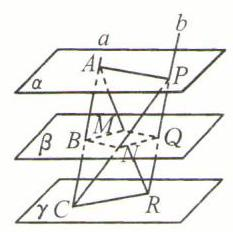
\includegraphics[width=0.4\textwidth]{bodyxb/src/bo_d20aucref24c73anc48g_153_422_714_233_232_0.jpg}}{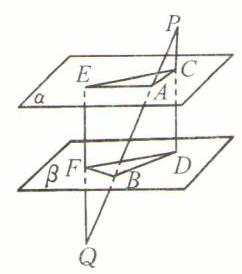
\includegraphics[width=0.4\textwidth]{bodyxb/src/bo_d20aucref24c73anc48g_153_912_666_242_274_0.jpg}}
    \begin{enumerate}
        \item 已知: 两条异面直线 $a,b$ 分别与三个平行平面 $\alpha ,\beta ,\gamma$ 相交于点 $A,B,C$ 和点 $P,Q,R$ ,又 ${AR},{CP}$ 与平面 $\beta$ 相交于点 $M,N$ (如左图),求证: ${MBNQ}$ 为平行四边形
        \begin{jieda}
            设$C,P,R$所确定平面为$\rho$，则$\rho \cap \beta = NQ, \rho \cap \gamma = AR$，根据面面平行的性质定理可知$NQ // CR$，同理可知$BM // CR$，因此$BM // NQ$，同理可知$BN // MQ$，因此${MBNQ}$ 为平行四边形.
        \end{jieda}
        \item 线段 ${PQ}$ 分别和两平行平面 $\alpha ,\beta$ 相交于点 $A,B$ ,两异面直线 ${PD},{QE}$ 分别和 $\alpha ,\beta$ 相交于点 $C,D$ 和点 $E,F$ (如右图). 若 ${AP} = {BQ}$ ,求证: $\bigtriangleup  {ACE}$ 的面积与 $\bigtriangleup  {DBF}$ 的面积相等
        \begin{jieda}
            ${S}_{\bigtriangleup {ACE}} = \dfrac{1}{2}{AE} \cdot  {AC} \cdot  \sin \angle {CAE},{S}_{\bigtriangleup {DBF}} = \dfrac{1}{2}{BF} \cdot  {BD} \cdot  \sin \angle {DBF}.\because \alpha //\beta$ ,在平面 ${PBD}$ 和 ${QAE}$ 中, ${AC}//$  ${BD}$ , ${AE}//{BF}$ , $\therefore \sin \angle {CAE} = \sin \angle {DBF}$ ； $\dfrac{AC}{BD} = \dfrac{PA}{PB} = \dfrac{PA}{{PA} + {AB}} = \dfrac{QB}{{QB} + {AB}} = \dfrac{QB}{QA} = \dfrac{BF}{AE}$ , $\therefore {S}_{\bigtriangleup {ACE}} = {S}_{\bigtriangleup {DBF}}$ , 证毕.
        \end{jieda}
    \end{enumerate}
\end{enumerate}

\begin{center}  \textbf{(B)} \end{center}
\begin{enumerate}
    \item \begin{enumerate}
        \item 已知平面 $\alpha //$ 平面 $\beta$ ,直线 $a,b$ 分别与平面 $\alpha ,\beta$ 所成角相等,则 $a,b$ 的位置关系是\blkda[3]{相交、平行或异面}
        \begin{jieda}
            在正方体 ${ABCD} - {A}^{\prime }{B}^{\prime }{C}^{\prime }{D}^{\prime }$ 中,取 $\alpha  =$ 平面 ${ABCD},\beta  =$ 平面 ${A}^{\prime }{B}^{\prime }{C}^{\prime }{D}^{\prime }$ ,直线 $\alpha  = A{B}^{\prime }$ ,当 $b = A{D}^{\prime }$ 时, $a,b$ 相交; 当 $b = D{C}^{\prime }$ 时, $a,b$ 平行; 当 $b = C{D}^{\prime }$ 时, $a,b$ 异面.
        \end{jieda}
        \item 若夹在两个平面间的三条平行线段相等,那么这两个平面的位置关系是\blkda[2]{平行或相交}
        \begin{jieda}
            显然,两平面平行时,夹在其间的平行线段都相等；两平面相交的例子是:在正方体 ${ABCD}$ - ${A}^{\prime }{B}^{\prime }{C}^{\prime }{D}^{\prime }$ 中,取 ${A}^{\prime }{B}^{\prime }$ 和 ${DC}$ 的中点 $M,N$ ,平行线段 ${A}^{\prime }D,{MN},{B}^{\prime }C$ 夹在平面 ${ABCD},{AB}{B}^{\prime }{A}^{\prime }$ 间,而这两个平面有交线 ${AB}$ . 
            
            \ps 对于本题,若平面 $\alpha ,\beta$ 之间有相等的平行线段 ${PQ},{RS},{TU},P,R,T \in  \alpha ,Q,S,U \in  \beta$ ,当 $P,R,T$ (或 $Q,S,U)$ 三点不共线时,必有 $\alpha //\beta$ .
        \end{jieda}
    \end{enumerate}
    \item 如图,在棱长为 $a$ 的正方体 ${ABCD} - {A}_{1}{B}_{1}{C}_{1}{D}_{1}$ 中
    \begin{center}
    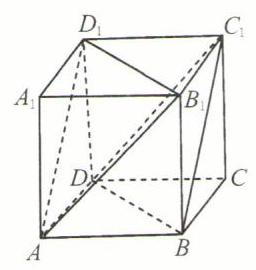
\includegraphics[width=0.2\textwidth]{bodyxb/src/bo_d20aucref24c73anc48g_153_362_1733_256_270_0.jpg}
    \end{center}
    \begin{enumerate}
        \item 求证:截面 ${BD}{C}_{1}//$ 截面 $A{B}_{1}{D}_{1}$
        \item 求截面 ${BD}{C}_{1}$ 与截面 $A{B}_{1}{D}_{1}$ 间的距离
    \end{enumerate}
    \begin{jieda}
        \begin{enumerate}
            \item 由 ${B}_{1}B\bot {D}_{1}D$ ,可知四边形 ${BD}{D}_{1}{B}_{1}$ 是平行四边形, $\therefore {BD}//{D}_{1}{B}_{1},{BD}//$ 平面 $A{B}_{1}{D}_{1}$ . 同理 $D{C}_{1}//$ 平面 $A{B}_{1}{D}_{1}$ ,又 ${BD} \cap  D{C}_{1} = D,\therefore$ 截面 ${BD}{C}_{1}//$ 截面 $A{B}_{1}{D}_{1}$ ,证毕.
            
            \item 连接 ${A}_{1}{C}_{1}$ 交 ${B}_{1}{D}_{1}$ 于 $M$ ,连接 ${AC}$ 交 ${BD}$ 于 $N$ ,连接 ${C}_{1}N$ ,在平面 ${AC}{C}_{1}{A}_{1}$ 中,作 ${MP} \bot  N{C}_{1}$ 于 $P$ . 不难证明, ${BD} \bot$ 平面 ${AC}{C}_{1}{A}_{1},\therefore {MP} \bot  {BD}$ ; 又 ${MP} \bot  N{C}_{1}$ , $\therefore {MP} \bot$ 截面 ${BD}{C}_{1},\therefore {MP}$ 就是两截面之间的距离. 如图,在 ${{Rt}} \bigtriangleup  {NM}{C}_{1}$ 中,由面积法, ${MP} = \dfrac{{MN} \cdot  M{C}_{1}}{N{C}_{1}} = \dfrac{a \cdot  \dfrac{\sqrt{2}}{2}a}{\dfrac{\sqrt{6}}{2}a} = \dfrac{\sqrt{3}}{3}a$ .
            
            \begin{center}
            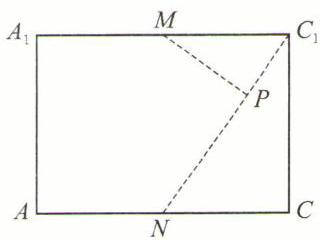
\includegraphics[width=0.2\textwidth]{bodyxb/src/bo_d20cdrf7aajc73bfmvhg_127_1104_754_321_242_0.jpg}
            \end{center}
        \end{enumerate}
    \end{jieda}
    \item 已知: ${AB}$ 与 ${CD}$ 为异面线段, ${CD} \subset$ 平面 $\alpha ,{AB}//\alpha ,M,N$ 分别是线段 ${AC}$ 和 ${BD}$ 的中点 (如图),求证: ${MN}//$ 平面 $\alpha$

    \begin{center}
    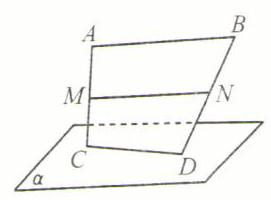
\includegraphics[width=0.2\textwidth]{bodyxb/src/bo_d20aucref24c73anc48g_153_876_1796_271_200_0.jpg}
    \end{center}
    \begin{jieda}
        连接 ${AD}$ 并取其中点 $P$ ,则可证得 ${MP}//{CD},{NP}//{AB}$ ,又 ${AB}//\alpha$ ,于是 ${MP}//\alpha ,{NP}//\alpha$ , 故平面 ${MNP}//\alpha$ ,从而 ${MN}//\alpha$ .
    \end{jieda}
\end{enumerate}


\subsection*{(二)二面角}

\subsubsection*{【典型题型和解题技巧】}

1. 二面角大小的计算.

二面角是立体几何中相当重要的内容, 有比较强的综合性. 计算二面角大小的方法主要有两种:

(1)直接法. 所谓直接法,就是直接作出二面角的平面角,经证明再进行计算.

常用的直接法又有三种:

\ding{172}定义法. 当点 $A$ 在二面角 $\alpha  - l - \beta$ 的棱 $l$ 上时,可过 $A$ 分别在 $\alpha ,\beta$ 内作棱 $l$ 的垂线 (射线) ${AB},{AC}$ ,由二面角平面角的定义,可知 $\angle {BAC}$ 就是二面角 $\alpha  - l - \beta$ 的平面角.

\textbf{例 1} 过 ${60}^{ \circ  }$ 的二面角 $\alpha  - l - \beta$ 的棱上一点 $O$ ,分别在 $\alpha ,\beta$ 内 $O$ 的同侧引两条射线 ${OP},{OQ}$ ,使 ${OP},{OQ}$ 与 $l$ 都成 ${45}^{ \circ  }$ 角,求 $\angle {POQ}$ 的余弦值.

\begin{center}
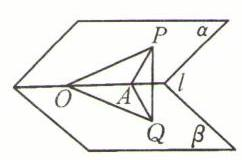
\includegraphics[width=0.2\textwidth]{bodyxb/src/bo_d20aucref24c73anc48g_154_1256_771_242_160_0.jpg}
\end{center}

\textbf{解} 

在 $l$ 上取一点 $A$ ,过 $A$ 分别在 $\alpha ,\beta$ 内作 $l$ 的垂线,与 ${OP},{OQ}$ 交于点 $P,Q$ ,则 $\angle {PAQ}$ 即二面角 $\alpha  - l - \beta$ 的平面角.

不妨设 ${OA} = 1$ ,则 ${AP} = {AQ} = 1$ ,则 ${OP} = {OQ} = \sqrt{2}$ .

又 $\angle {PAQ} = {60}^{ \circ  },\therefore {PQ} = 1$ ,于是利用余弦定理,得 $\cos \angle {POQ} = \dfrac{2 + 2 - 1}{2 \cdot  \sqrt{2} \cdot  \sqrt{2}} = \dfrac{3}{4}$ .

\ding{173}三垂线定理法. 当点 $A$ 在二面角 $\alpha  - l - \beta$ 的一个面 $\alpha$ 内时,可作 ${AO}\bot \beta$ 于点 $O$ ,再作 ${OB} \bot  l$ 于点 $B$ ,连接 ${AB}$ ,则由三垂线定理,得 ${AB} \bot  l$ ,故 $\angle {ABO}$ 就是二面角 $\alpha  - l - \beta$ 的平面角或其补角.

\textbf{例 2} 已知 $P,Q,M$ 分别是 ${45}^{ \circ  }$ 的二面角 $\alpha  - l - \beta$ 的面 $\alpha ,\beta$ 和棱 $l$ 上的点,直线 ${MQ}$ 是直线 ${PQ}$ 在 $\beta$ 上的射影. 若 ${PQ}$ 和 $\beta$ 成 $\varphi$ 角, $l$ 和 ${MQ}$ 成 $\theta$ 角, ${PM} = a$ ,求 ${PQ}$ 的长.

\textbf{解}

\begin{center}
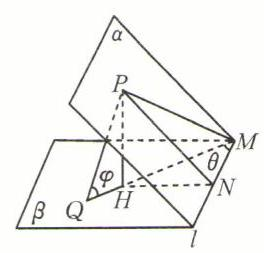
\includegraphics[width=0.2\textwidth]{bodyxb/src/bo_d20aucref24c73anc48g_154_1234_1512_264_253_0.jpg}
\end{center}

作 ${PH} \bot  \beta$ 于点 $H,\because {MQ}$ 是 ${PQ}$ 在 $\beta$ 上的射影，$\therefore H$ 在 ${MQ}$ 上，作 ${HN} \bot  l$ 于点 $N$ ,连接 ${PN}$ ,则由三垂线定理可知 ${PN} \bot  l$，$\therefore \angle {PNH}$ 是二面角 $\alpha  - l - \beta$ 的平面角,即 $\angle {PNH} = {45}^{ \circ  }$ .

设 ${PQ} = x$ ,则 ${NH} = {PH} = x\sin \varphi ,{PN} = \sqrt{2}x\sin \varphi$，${MN} = {NH}\cot \theta  = x\sin \varphi  \cdot  \cot \theta .$

在 ${{Rt}} \bigtriangleup  {PMN}$ 中, $\because P{M}^{2} = P{N}^{2} + M{N}^{2}$，$\therefore {a}^{2} = {x}^{2}{\sin }^{2}\varphi  \cdot  \left( {2 + {\cot }^{2}\theta }\right)$ ,故 ${PQ} = x = \dfrac{a}{\sin \varphi  \cdot  \sqrt{2 + {\cot }^{2}\theta }}$

\ding{174}垂面法.

当点 $A$ 在二面角 $\alpha  - {OP} - \beta$ 内时,可作 ${AB} \bot  \alpha$ 于点 $B$ ,作 ${AC} \bot  \beta$ 于点 $C$. 设过 ${AB},{AC}$ 的平面与 ${OP}$ 交于点 $O$ ,连接 ${OB},{OC}$.

\begin{center}
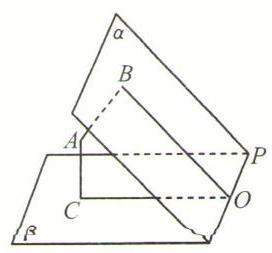
\includegraphics[width=0.2\textwidth]{bodyxb/src/bo_d20aucref24c73anc48g_154_1227_1920_272_253_0.jpg}
\end{center}

$\because {AB} \bot  \alpha ,\therefore {AB} \bot  {OP}$，又 $\because {AC} \bot  \beta ,\therefore {AC} \bot  {OP}$ ,而 ${AB} \cap  {AC} = A$ ,

$\therefore {OP} \bot$ 平面 ${ABOC}$ ,于是, ${OP} \bot  {OB},{OP} \bot  {OC}$，$\therefore \angle {BOC}$ 就是二面角 $\alpha  - {OP} - \beta$ 的平面角.

由于平面 ${ABOC}$ 和棱 ${OP}$ 垂直,故此法称为 “垂面法”.

\textbf{例 3} 已知 $P$ 是角度为 $\theta$ 的锐二面角 $\alpha  - l - \beta$ 内一点，若点 $P$ 到 $\alpha ,\beta$ 的距离分别为 $a,b$ ,求点 $P$ 到棱 $l$ 的距离.

\textbf{解}

作 ${PA} \bot  \alpha$ 于点 $A,{PB} \bot  \beta$ 于点 $B$ ,设过 ${PA},{PB}$ 的平面交 $l$ 于点 $C$，则 $l\bot$ 平面 ${APBC}$

\begin{center}
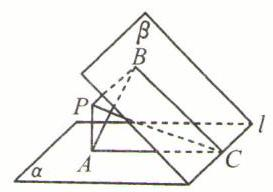
\includegraphics[width=0.2\textwidth]{bodyxb/src/bo_d20aucref24c73anc48g_155_1127_664_273_192_0.jpg}
\end{center}

$\therefore l \bot  {AC},l \bot  {BC}$ ,于是 $\angle {ACB}$ 是二面角 $\alpha  - l - \beta$ 的平面角,即 $\angle {ACB} = \theta$ .

连接 ${PC}$ ,则 $l\bot {PC}$，$\therefore {PC}$ 即为点 $P$ 到 $l$ 的距离,连接 ${AB}$，$\because \angle {APB} = {180}^{ \circ  } - \theta$ ,并结合 ${PA} = a,{PB} = b$ ,便得 ${AB} = \sqrt{{a}^{2} + {b}^{2} + {2ab}\cos \theta }$ .

显然, $P,A,C,B$ 四点共圆,且 ${PC}$ 是圆的直径,根据正弦定理,得 ${PC} = \dfrac{AB}{\sin \theta }$  $= \dfrac{\sqrt{{a}^{2} + {b}^{2} + {2ab}\cos \theta }}{\sin \theta }.$

(2)间接法. 当二面角的平面角不易作出时,可考虑运用间接法.

设 $\alpha$ 内的一个封闭几何图形的面积为 $S$ ,此几何图形在 $\beta$ 上的射影面积为 ${S}^{\prime }$ ,二面角 $\alpha  - l$  $- \beta$ 的大小为 $\theta$ ,可以证明 $\left| {\cos \theta }\right|  = \dfrac{{S}^{\prime }}{S}$ (证明略). 由于运用了射影的手段,因此该方法也称为射影法.

\textbf{例 4} 设 $E$ 为正方体 ${ABCD} - {A}_{1}{B}_{1}{C}_{1}{D}_{1}$ 的棱 $C{C}_{1}$ 的中点，求平面 $A{B}_{1}E$ 和底面 ${A}_{1}{B}_{1}{C}_{1}{D}_{1}$ 所成锐二面角的余弦值.

\begin{center}
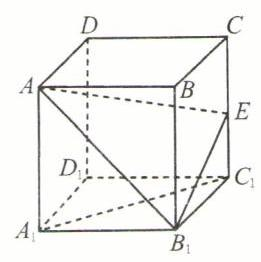
\includegraphics[width=0.2\textwidth]{bodyxb/src/bo_d20aucref24c73anc48g_155_1144_1527_261_262_0.jpg}
\end{center}

\textbf{解} 

连接 ${A}_{1}{C}_{1}$ ,显然, $\bigtriangleup {A}_{1}{B}_{1}{C}_{1}$ 是 $\bigtriangleup A{B}_{1}E$ 的底面上的射影,设正方体的棱长为 2,则 $A{B}_{1} = 2\sqrt{2},{B}_{1}E = \sqrt{5},{AE} = 3$ ,于是 $\cos \angle {B}_{1}{AE} =$  $\dfrac{A{B}_{1}^{2} + A{E}^{2} - {B}_{1}{E}^{2}}{2 \cdot  A{B}_{1} \cdot  {AE}} = \dfrac{8 + 9 - 5}{2 \cdot  2\sqrt{2} \cdot  3} = \dfrac{\sqrt{2}}{2},\therefore \angle {B}_{1}{AE} = {45}^{ \circ  }$ .

故 ${S}_{\bigtriangleup {B}_{1}{AE}} = \dfrac{1}{2} \cdot  2\sqrt{2} \cdot  3 \cdot  \sin {45}^{ \circ  } = 3$，而 ${S}_{\bigtriangleup {A}_{1}{B}_{1}{C}_{1}} = 2$ ,于是,平面 $A{B}_{1}E$ 与底面 ${A}_{1}{B}_{1}{C}_{1}{D}_{1}$ 所成锐二面角 $\theta$ 的余弦值为 $\cos \theta  =$  $\dfrac{{S}_{\bigtriangleup {A}_{1}{B}_{1}{C}_{1}}}{{S}_{\bigtriangleup A{B}_{1}E}} = \dfrac{2}{3}.$

2. 平面图形的 “翻折” 问题.

将平面图形进行翻折,研究折后空间元素的数量或位置关系,这是一类特殊的题型.

在解此类问题时, 通常可以同时画出折前的平面图形和折后的空间图形, 进行对照分析. 凡在折后的图形中添加的辅助线,都应在折前的平面图形中相应画出,这样做,对有关线段、角度的数量关系容易作出正确的判断.

\textbf{例 5} Rt $\bigtriangleup {ABC}$ 和 Rt $\bigtriangleup {BCD}$ 有公共边 ${BC}$ ,其中 ${AB} = {AC},\angle {BAC} = {90}^{ \circ  },\angle {BCD} = {90}^{ \circ  }$ , $\angle {CBD} = {30}^{ \circ  },{BC} = \sqrt{6}$ [如图(1)]. 今以 ${BC}$ 为棱折成大小为 $\theta \left( {0 < \theta  < \dfrac{\pi }{2}}\right)$ 的二面角 [如图(2)].

(1)求翻折后线段 ${AD}$ 的长；

(2)当点 $A$ 在平面 ${BCD}$ 上的射影在 ${BD}$ 上时,求 $\theta$ 的余弦值.

\begin{center}
    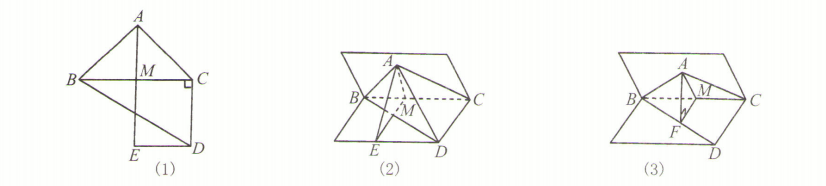
\includegraphics[width=0.75\linewidth]{bodyxb//src/ermianjiao1.png}
\end{center}

\textbf{解}

(1)在面 ${ABC}$ 内,作 ${AM}\bot {BC},M$ 为垂足,在面 ${BCD}$ 内过点 $M$ 作 ${CD}$ 的平行线,过点 $D$ 作 ${BC}$ 的平行线,所作两直线交于点 $E$ ,连接 ${AE}$ .

显然, $\angle {AME}$ 是二面角 $A - {BC} - D$ 的平面角,故 $\angle {AME} = \theta$ .

由 ${BC} \bot  {AM},{BC} \bot  {EM}$ 知, ${BC} \bot$ 平面 ${AME}$ ,而 ${DE}//{BC}$ ,

$\therefore {DE} \bot$ 平面 ${AME}$ ,故 ${DE} \bot  {AE}$. $\because {BC} = \sqrt{6},\therefore {AM} = \dfrac{\sqrt{6}}{2},{EM} = {CD} = \sqrt{2}$ ,

于是 $A{E}^{2} = \dfrac{3}{2} + 2 - 2 \cdot  \dfrac{\sqrt{6}}{2} \cdot  \sqrt{2}\cos \theta  = \dfrac{7}{2} - 2\sqrt{3}\cos \theta$ ,

$A{D}^{2} = A{E}^{2} + D{E}^{2} = \dfrac{7}{2} - 2\sqrt{3}\cos \theta  + \dfrac{3}{2} = 5 - 2\sqrt{3}\cos \theta ,\therefore {AD} = \sqrt{5 - 2\sqrt{3}\cos \theta }$ .

(2)如图(3),作 ${AF} \bot$ 平面 ${BCD},F$ 为垂足,由题设,点 $F$ 在 ${BD}$ 上.

$\because {AM} \bot  {BC},\therefore $ 由三垂线定理,得 ${MF} \bot  {BC}$ ,于是 $\angle {AMF} = \theta$ .

在 ${{Rt}} \bigtriangleup  {AFM}$ 中, $\because {AM} = \dfrac{\sqrt{6}}{2},{FM} = \dfrac{1}{2}{CD} = \dfrac{\sqrt{2}}{2},\therefore \cos \theta  = \dfrac{FM}{AM} = \dfrac{\sqrt{3}}{3}$ .

\subsubsection*{【训练题】}

\begin{center}  \textbf{(A)} \end{center}

\begin{enumerate}
    \item 已知二面角 $\alpha  - a - \beta$ 的大小为 $\theta \left( {\dfrac{\pi }{2} < \theta  < \pi }\right) ,{AB} \subset  \alpha ,{CD} \subset  \beta$ ,且 ${AB} \bot  a,{CD} \bot  a$ . 若 ${AB}$ 与 ${CD}$ 所成的角为 $\varphi$ ,则 \dotfill{(\kh{D})}
    \xx{$\varphi  = \theta$}{$\varphi  = \theta  - \dfrac{\pi }{2}$}{$\varphi  = \theta  + \dfrac{\pi }{2}$}{$\varphi  = \pi  - \theta$}
    \begin{jieda}
        空间内两直线所成的角的取值范围是 $\left\lbrack  {0,\dfrac{\pi }{2}}\right\rbrack$ ,由题意 $\varphi  + \theta  = \pi ,\therefore \varphi  = \pi  - \theta$ 
    \end{jieda}
    
    \item 自二面角内一点分别向它的两个半平面作垂线段,则这两条垂线段所夹的角和二面角的平面角之间的关系是\dotfill{(\kh{C})}
    \xx{相等}{互为余角}{互为补角}{和等于 ${360}^{ \circ  }$}
    \begin{jieda}
        记二面角为 $\alpha  - l - \beta$ ,过其内一点 $P$ 作 ${PA}\bot \alpha ,{PB}\bot \beta$ . 垂足为 $A,B$ . 若 $A,B$ 分别在两个半平面内,在 $\alpha$ 内作 ${AQ}\bot l$ 于 $Q$ ,连接 ${BQ}$ ,易证 $l\bot$ 平面 ${PAQB},\therefore \angle {AQB}$ 就是二面角 $\alpha  - l - \beta$ 的平面角,四边形 ${PAQB}$ 中, $\angle {AQB}$ 和两条垂线所夹的角 $\angle {APB}$ 互为补角. 若 $A,B$ 中恰有一点在其中一个半平面内,可以验证该结论依然成立.
    \end{jieda}
    
    \item 已知直线 $m \subset$ 平面 $\alpha$ ,二面角 $\alpha  - l - \beta$ 的大小为 $\varphi$ ,且 $m$ 与 $\beta$ 所成角为 $\theta$ ,则\dotfill{(\kh{A})}
    \xx{$\varphi  \geq  \theta$}{$\varphi  < \theta$}{当 $\varphi  > \dfrac{\pi }{2}$ 时, $\varphi  > \theta$ ; 当 $\varphi  \leq  \dfrac{\pi }{2}$ 时, $\varphi  \leq  \theta$}{$\varphi$ 与 $\theta$ 的大小关系不能确定}
    \begin{jieda}
        $\theta  \in  \left\lbrack  {0,\dfrac{\pi }{2}}\right\rbrack$ ,故 $\varphi  \geq  \dfrac{\pi }{2}$ 或 $\theta  = 0$ 时,都有 $\varphi  \geq  \theta$ . 当 $\varphi  < \dfrac{\pi }{2}$ 且 $\theta  \neq  0$ 时,记 $m \cap  l = A$ ,再取 $m$ 上异于 $A$ 的一点 $P \in$  $m \subset  \alpha$ ；点 $P$ 在平面 $\beta$ 上的射影是 $Q$ ,则 $\angle {PAQ}$ 就是 $m$ 与 $\beta$ 所成的角；在平面 $\beta$ 内作 ${QB}\bot l$ 于 $B$ ,由三垂线定理, ${PB}\bot l$ 于 $B,\therefore \angle {PBQ}$ 就是二面角 $\alpha  - l - \beta$ 的平面角,而 $\sin \varphi  = \dfrac{PQ}{PB} \geq  \dfrac{PQ}{PA} = \sin \theta ,\therefore \varphi  \geq  \theta$ (等号当且仅当 ${PB} = {PA}$ 即 $m$  $\bot  l$ 时成立). 综上 $\varphi  \geq  \theta$ 总是成立.
    \end{jieda}
    \item 在正方体 ${ABCD} - {A}_{1}{B}_{1}{C}_{1}{D}_{1}$ 中,截面 ${A}_{1}{BD}$ 与底面 ${ABCD}$ 所成二面角 ${A}_{1} - {BD} - A$ 的正切值等于\dotfill{(\kh{C})}
    \xx{$\dfrac{\sqrt{3}}{3}$}{$\dfrac{\sqrt{2}}{2}$}{$\sqrt{2}$}{$\sqrt{3}$}
    \begin{jieda}
        取 ${BD}$ 中点 $M$ ,连接 ${AM}\text{ 、 }{A}_{1}M$ . 等腰三角形 ${ABD}$ 中, ${AM}$ 是底边上的中线, $\therefore {AM}\bot {BD}$ 于 $M$ ,同理可证 ${A}_{1}M\bot {BD}$ 于 $M,\therefore \angle {A}_{1}{MA}$ 就是二面角 ${A}_{1} -$  ${BD} - A$ 的平面角. 又 ${A}_{1}A \bot$ 平面 ${ABCD},\therefore {A}_{1}A \bot  {AM},\therefore \tan \angle {A}_{1}{MA} = \dfrac{{A}_{1}A}{MA} = \dfrac{1}{\dfrac{1}{2}\sqrt{2}} = \sqrt{2}$
    \end{jieda}
    \item 过正方形 ${ABCD}$ 的顶点 $A$ 作线段 ${AP} \bot$ 面 ${ABCD}$ ,且 ${AP} = {AB}$ ,则面 ${ABP}$ 与面 ${CDP}$ 所成锐二面角的度数是\dotfill{(\kh{B})}
    \xx{${30}^{ \circ  }$}{${45}^{ \circ  }$}{${60}^{ \circ  }$}{${90}^{ \circ  }$}
    \begin{jieda}
        在平面 ${PAB}$ 内,过点 $P$ 作直线 $l//{AB},P \in  l$ 和 ${AB}$ 确定的平面, $\therefore l \subset$ 平面 ${PAB}$ . 又 $l//{AB}//{DC}$ ,同理可证 $l \subset$ 平面 ${PDC},\therefore l$ 就是所求二面角的棱. 又 ${BA} \bot  {PA}\text{ 、 }{BA} \bot  {DA},\therefore {BA} \bot$ 平面 ${PAD},\therefore l \bot$ 平面 ${PAD}$ , $\therefore \angle {APD}$ 就足所求二面角的平面角,是等腰直角三角形 ${PAD}$ 的底角,即 ${45}^{ \circ  }$
    \end{jieda}
    \item 已知等边三角形 ${ABC}$ 的边长为 1,沿 ${BC}$ 边上的高将它折成直二面角后,点 $A$ 到 ${BC}$ 的距离为 \dotfill{(\kh{A})}
    \xx{$\dfrac{\sqrt{14}}{4}$}{$\dfrac{\sqrt{2}}{2}$}{1}{$\dfrac{\sqrt{3}}{2}$}
    \begin{jieda}
        记折叠前、后,线段 ${BC}$ 的中点分别为 $D,E$ . 折叠后, ${AD}\bot {BD},{AD}\bot {CD}$ ,
        
        $\therefore {AD} \bot$ 平面 ${BDC}$ , $\therefore$ 二面角 $B - {DA} - C$ 的一个平面角是 $\angle {BDC} = {90}^{ \circ  }, \bigtriangleup  {BDC}$ 是等腰直角三角形. 折叠后,等腰三角形 ${ABC}$ 中, ${AE}$ 是底边 ${BC}$ 上的中线,故 ${AE} \bot  {BC},{AE}$ 即为所求距离. $\operatorname{Rt} \bigtriangleup  {ADE}$ 中, ${AD} = \dfrac{\sqrt{3}}{2},{DE} = \dfrac{DB}{\sqrt{2}} = \dfrac{\sqrt{2}}{4},{AE}$  $= \sqrt{A{D}^{2} + D{E}^{2}} = \dfrac{\sqrt{14}}{4}.$
    \end{jieda}
    
    \item 将锐角 $\angle {QMN} = {60}^{ \circ  }$ ,边长 ${MN} = a$ 的菱形 ${MNPQ}$ 沿对角线 ${NQ}$ 折成 ${60}^{ \circ  }$ 的二面角,则 ${MP}$ 与 ${NQ}$ 间的距离等于\dotfill{(\kh{B})}
    \xx{$\dfrac{\sqrt{3}}{2}a$}{$\dfrac{3}{4}a$}{$\dfrac{\sqrt{6}}{4}a$}{$\dfrac{\sqrt{3}}{4}a$}
    \begin{jieda}
        折叠后,记线段 ${NQ}$ 中点为 $R$ ,连接 $\bigtriangleup {MRP}$ 三边,并作 ${RS}\bot {MP}$ 于 $S$ . 先证 ${RS}$ 即为所求: 由于 ${RM}$ 、 ${RP}$ 相交, 且都与 ${NQ}$ 垂直, $\therefore {NQ} \bot$ 平面 ${MRP},\therefore {NQ} \bot  {RS},$ 又 ${RS} \bot  {MP},\therefore$ 线段 ${RS}$ 是 ${MP}$ 与 ${NQ}$ 的公垂线段. 再求 ${RS}$ 的长度:显然二面角 $M - {NQ} - P$ 的一个平面角是 $\angle {MRP} = {60}^{ \circ  }$ ,又 ${RM} = {RP},\therefore \bigtriangleup {MRP}$ 是等边三角形, ${RS}$ 是它的高, ${RS} = \dfrac{\sqrt{3}}{2}{RM} = \dfrac{\sqrt{3}}{2} \cdot  \dfrac{\sqrt{3}}{2} \cdot  {MN} = \dfrac{3}{4}a$ .
    \end{jieda}
    
    \item 已知 $E,F$ 分别是正方体 ${ABCD} - {A}_{1}{B}_{1}{C}_{1}{D}_{1}$ 的棱 ${BC},C{C}_{1}$ 的中点,则截面 ${AEF}{D}_{1}$ 与底面 ${ABCD}$ 所成二面角的正弦值等于\dotfill{(\kh{C})}.
    \xx{$\dfrac{2\sqrt{2}}{3}$}{$\dfrac{\sqrt{2}}{3}$}{$\dfrac{\sqrt{5}}{3}$}{$\dfrac{2}{3}$}
    \begin{jieda}
        过$D$做$AE$的垂线，垂足为$H$，$\angle{DHD_1}$为二面角的平面角，$DH = \dfrac{2\sqrt{5}}{5}$，$D_1H = \sqrt{1+\dfrac{4}{5}} = \dfrac{3\sqrt{5}}{5}$，故目标正弦值为$\dfrac{\sqrt{5}}{3}$.
    \end{jieda}
    \item 
    \begin{enumerate}
        \item 已知二面角 $\alpha  - l - \beta$ 为 ${60}^{ \circ  },\alpha$ 内一点 $A$ 到棱 $l$ 的距离为 $2\sqrt{3}$ ,则 $A$ 到 $\beta$ 的距离为\blkda{3}
        \begin{jieda}
            记点 $A$ 在平面 $\beta$ 上的射影是 $B$ ,作 ${BC} \bot$ 棱 $l$ 于 $C$ ,连接 ${AC}$ . 由三垂线定理, $l \bot  {AC}$

            $\angle {ACB}$ 就是二面角 $\alpha  - l - \beta$ 的平面角, $A$ 到 $\beta$ 的距离 ${AB} = {AC} \cdot  \sin \angle {ACB} = 2\sqrt{3} \cdot  \sin {60}^{ \circ  } = 3$
        \end{jieda}
        \item 两个等腰三角形 ${ABC}$ 与 ${DBC}$ 的公共底边 ${BC} = {16}{{cm}},{AB} = {17}{{cm}},{DB}\bot {DC}$ ,且二面角 $A - {BC} - D$ 成 ${60}^{ \circ  }$ ,则 $A,D$ 间的距离等于\blkda{13} ${{cm}}$
        \begin{jieda}
            取线段 ${BC}$ 中点为 $E$ ,连接 $\bigtriangleup  {AED}$ 三边. 由于 ${EA}$ , ${ED}$ 都与 ${BC}$ 垂直

            $\angle {AED}$ 就是二面角 $A - {BC} - D$ 的平面角, ${EA} = \sqrt{B{A}^{2} - B{E}^{2}} = {15}{{cm}},{ED} = {EB} = 8{{cm}}$ ,由余弦定理, ${AD} =$  $\sqrt{E{A}^{2} + E{D}^{2} - 2 \cdot  {EA} \cdot  {ED} \cdot  \cos \angle {AED}} = {13}{{cm}}.$
        \end{jieda}
    \end{enumerate}
    \item \begin{enumerate}
        \item 已知 $\bigtriangleup {ABC}$ 为等边三角形, ${PA} \bot$ 面 ${ABC}$ ,且 ${PA} = \dfrac{1}{2}{AC}$ ,则二面角 $P - {BC} - A$ 的度数为\blkda{${30}^{ \circ  }$}
        \begin{jieda}
            不妨设 $\bigtriangleup {ABC}$ 的边长为 2,则 ${PA} = 1$ . 取 ${BC}$ 中点 $D$ ,连接 ${DA},{DP}$ ,则 ${DA} = \sqrt{3}$ . 由三垂线定理, ${BC} \bot$  ${AD} \Longrightarrow  {BC} \bot  {PD}$ ,故 $\angle {PDA}$ 就是二面角 $P - {BC} - A$ 的平面角. $\tan \angle {PDA} = \dfrac{PA}{DA} = \dfrac{\sqrt{3}}{3},\therefore \angle {PDA} = {30}^{ \circ  }$
        \end{jieda}
        \item 已知 $P$ 为二面角内一点,且 $P$ 到其两个半平面的距离都等于 $P$ 到棱的距离的一半, 则这个二面角的度数为\blkda{${60}^{ \circ  }$}
        \begin{jieda}
            记二面角为 $\alpha  - l - \beta$ ,点 $P$ 在 $\alpha$ 、 $\beta$ 上的射影分别为 $A$ 、 $B$ ,平面 ${PAB} \cap  l = C$ .易证: $l \bot$ 平面 ${PACB}$ ,
            
            $\therefore l \bot  {CA},l \bot  {CB},l \bot  {CP}$ ,故 $\angle {ACB}$ 就是二面角 $\alpha  - l - \beta$ 的平面角. 在 ${{Rt}} \bigtriangleup  {PCA}$ 中, $\sin \angle {PCA} = \dfrac{PA}{PC} = \dfrac{1}{2}$ ,
            
            $\therefore \angle {PCA} = {30}^{ \circ  }$ ,同理 $\angle {PCB} = {30}^{ \circ  },\therefore \angle {ACB} = {60}^{ \circ  }$ .
        \end{jieda}
        \item 已知 $P$ 为锐二面角 $\alpha  - l - \beta$ 内一点,且 $P$ 到面 $\alpha ,\beta$ 及棱 $l$ 的距离之比为 $1 : \sqrt{2} : 2$ ,则此二面角的度数为\blkda{${75}^{ \circ  }$}
        \begin{jieda}
            记点 $P$ 在 $\alpha$ 、 $\beta$ 上的射影分别为 $A$ 、 $B$ ,平面 ${PAB} \cap  l = C$ .和第(2)小问类似,易知 $\angle {ACB}$ 就是二面角 $\alpha  - l$  $- \beta$ 的平面角,且 $\sin \angle {PCA} = \dfrac{PA}{PC} = \dfrac{1}{2} \Longrightarrow  \angle {PCA} = {30}^{ \circ  },\sin \angle {PCB} = \dfrac{PB}{PC} = \dfrac{\sqrt{2}}{2} \Longrightarrow  \angle {PCB} = {45}^{ \circ  },\therefore \angle {ACB} = {75}^{ \circ  }$ .
        \end{jieda}
        \item 过二面角 $\alpha  - l - \beta$ 内一点 $P$ 作 ${PA}\bot \alpha$ 于 $A$ ,作 ${PB}\bot \beta$ 于 $B$ ,其中 $A$ , $B$ 分别位于半平面 $\alpha$ 内和半平面 $\beta$ 内. 若 ${PA} = 5,{PB} = 8,{AB} = 7$ ,则二面角 $\alpha  - l - \beta$ 的度数为\blkda{${120}^{ \circ  }$}
        \begin{jieda}
            由余弦定理, $\cos \angle {APB} = \dfrac{P{A}^{2} + P{B}^{2} - A{B}^{2}}{2 \cdot  {PA} \cdot  {PB}} = \dfrac{1}{2},\therefore \cos \angle {APB} = {60}^{ \circ  }$ 
            
            二面角 $\alpha  - l - \beta$ 的平面角与 $\angle {APB}$ 互补,故该二面角为 ${120}^{ \circ  }$
        \end{jieda}
    \end{enumerate}
    \item \begin{enumerate}
        \item 已知正方形 ${ABCD}$ 与正方形 ${ABEF}$ 所成的二面角 $D - {AB} - F$ 的大小为 ${60}^{ \circ  }$ (如图), 则异面直线 ${AD}$ 与 ${BF}$ 所成角的余弦值为\blkda{$\dfrac{\sqrt{2}}{4}$}
        \begin{center}
        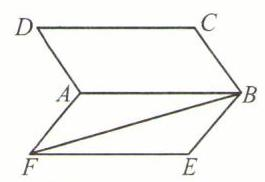
\includegraphics[width=0.2\textwidth]{bodyxb/src/bo_d20aucref24c73anc48g_158_318_603_265_182_0.jpg}
        \end{center}
        \begin{jieda}
            记正方形边长为 1,则 ${BC} = 1,{BF} = \sqrt{2},{AD}//{BC}$ ,故 ${AD}$ 与 ${BF}$ 所成角即 $\angle {CBF}$ 或其补角. ${AB}\bot {AD}$ , ${AB} \bot  {AF}$ ,故 $\angle {DAF}$ 就是二面角 $D - {AB} - F$ 的平面角. 另 ${AB} \bot$ 平面 ${DAF},\therefore {AB} \bot  {DF}$ ,又 ${DC}//{AB},\therefore {DC}\bot {DF}$ . 易知, $\bigtriangleup {DAF}$ 是等边三角形, $\therefore \bigtriangleup {FDC}$ 是等腰直角三角形, ${FC} = \sqrt{2}$ . 在 $\bigtriangleup {CBF}$ 中使用余弦定理, $\cos \angle {CBF} = \dfrac{B{C}^{2} + B{F}^{2} - C{F}^{2}}{2 \cdot  {BC} \cdot  {BF}} = \dfrac{\sqrt{2}}{4}.$
        \end{jieda}
        \item 已知边长为 $a$ 的菱形 ${ABCD}$ 中, $\angle {BAD} = {30}^{ \circ  }$ ,今沿对角线 ${AC}$ 将菱形折成 ${60}^{ \circ  }$ 的二面角 ${B}^{\prime } - {AC} - D$ (如图),则 ${AC}$ 与 $B{B}^{\prime }$ 间的距离等于\blkda{$\dfrac{\sqrt{6} - \sqrt{2}}{8}a$}
        \begin{center}
        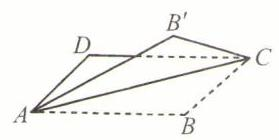
\includegraphics[width=0.2\textwidth]{bodyxb/src/bo_d20aucref24c73anc48g_158_709_643_279_140_0.jpg}
        \end{center}
        \begin{jieda}
            折叠后,记线段 ${AC}$ 中点为 $E$ ,连接 $\bigtriangleup {B}^{\prime }{EB}$ 三边,并作 ${EF}\bot {B}^{\prime }B$ 于 $F$ . 先证 ${EF}$ 即为所求:由于 $E{B}^{\prime },{EB}$ 相交,且都与 ${AC}$ 垂直, $\therefore {AC} \bot$ 平面 ${B}^{\prime }{EB},\therefore {AC} \bot  {EF}$ ,又 ${EF} \bot  B{B}^{\prime },\therefore$ 线段 ${EF}$ 是 ${AC}$ 与 $B{B}^{\prime }$ 的公垂线段. 再求 ${EF}$ 的长度: 显然二面角 ${B}^{\prime } - {AC} - B$ 的一个平面角是 $\angle {B}^{\prime }{EB} = {180}^{ \circ  } - {60}^{ \circ  } = {120}^{ \circ  }$ ,又 $E{B}^{\prime } =$  ${EB},\therefore {EF} = \dfrac{1}{2}{EB} = \dfrac{1}{2}{AB} \cdot  \sin {15}^{ \circ  } = \dfrac{\sqrt{6} - \sqrt{2}}{8}a$
        \end{jieda}
    \end{enumerate}
    \item \begin{enumerate}
        \item 在正方体 ${ABCD} - {A}_{1}{B}_{1}{C}_{1}{D}_{1}$ 中,求二面角 $A - D{B}_{1} - C$ 的大小
        \begin{jieda}
            平面$ACB_1$垂直于平面$ADB_1$和平面$CDB_1$，直线$BD_1$过平面$ACB_1$的中心$O$，故$\angle{AOC}$即为二面角$A - D{B}_{1} - C$的平面角，为$120^{\circ}$
        \end{jieda}
        \item 已知 $P$ 是二面角 $\alpha  - {AB} - \beta$ 棱上一点,过 $P$ 分别在 $\alpha ,\beta$ 内引射线 ${PM},{PN}$ ,且 $\angle {BPM} = \angle {BPN} = {45}^{ \circ  },\angle {MPN} = {60}^{ \circ  }$ (如图),求此二面角的度数
        \begin{center}
        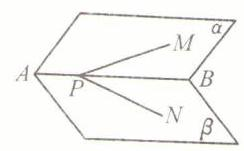
\includegraphics[width=0.2\textwidth]{bodyxb/src/bo_d20aucref24c73anc48g_158_1113_629_244_151_0.jpg}
        \end{center}
        \begin{jieda}
            根据三余弦定理可知$\angle{BPM} = 45^{\circ}$，取$PM = PN = 1$，做$MO \bot AB$，则$NO \bot AB$，$\angle{MON}$即为二面角的平面角，$MO = NO = \dfrac{\sqrt{2}}{2}$，$MN = 1$，故$\angle{MON}$为直角.
        \end{jieda}
        \item 已知 ${{Rt}} \bigtriangleup  {ABC}$ 的斜边 ${AB}$ 在平面 $\alpha$ 内, ${AC}$ , ${BC}$ 分别和 $\alpha$ 成 ${30}^{ \circ  }$ , ${45}^{ \circ  }$ 角,求平面 ${ABC}$ 与平面 $\alpha$ 所成的锐二面角
        \begin{jieda}
            记点 $C$ 在平面 $\alpha$ 上的射影是点 $D$ ,连接 ${DA}$ , ${DB}$ . 记 ${CD} = h$ ,则 ${AD} = \sqrt{3}h,{AC} = {2h};{BD} = h,{BC} = \sqrt{2}h,\therefore {AB}$  $= \sqrt{6}h$ . 
            
            在 $\bigtriangleup {ACB}$ 中作 ${CE}\bot {AB}$ 于 $E$ ,连接 ${DE}$ ,由三垂线定理: ${CE}\bot {AB} \Longrightarrow  {DE}\bot {AB},\therefore \angle {CED}$ 就是二面角 $C - {AB} - D$ 的平面角. ${CE} = \dfrac{{CB} \cdot  {CA}}{AB} = \dfrac{2}{3}\sqrt{3}h$ (面积法), $\sin \angle {CED} = \dfrac{CD}{CE} = \dfrac{\sqrt{3}}{2}$ ,故 $\angle {CED} = {60}^{ \circ  }$ . 
        \end{jieda}
    \end{enumerate}
    \item 
    \begin{enumerate}
        \item 已知 ${{Rt}}\bigtriangleup {ABC}$ 在平面 $\alpha$ 内,斜边 ${AB}$ 在 ${30}^{ \circ  }$ 的二面角 $\alpha  - {AB} - \beta$ 的棱上 (如图). 若 ${AC} = 5,{BC} = {12}$ ,求点 $C$ 到平面 $\beta$ 的距离

        \begin{center}
        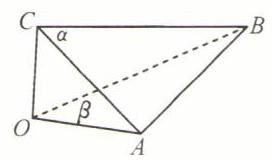
\includegraphics[width=0.2\textwidth]{bodyxb/src/bo_d20aucref24c73anc48g_158_477_1301_272_160_0.jpg}
        \end{center}

        \begin{jieda}
            设点 $C$ 在平面 $\beta$ 内的射影是点 $O$ ,在平面 ${ABC}$ 中,作 ${CD} \bot  {AB}$ 于 $D$ ,连接 ${OD}$ . 由三垂线定理: ${CD} \bot  {AB} \Longrightarrow  {OD} \bot$  ${AB},\therefore \angle {CDO}$ 就是二面角 $\alpha  - {AB} - \beta$ 的平面角. ${AB} = \sqrt{A{C}^{2} + B{C}^{2}} = {13},{CD} = \dfrac{{CA} \cdot  {CB}}{AB} = \dfrac{60}{13},\therefore {CO} = {CD} \cdot  \sin \angle {CDO} = \dfrac{30}{13}.$
        \end{jieda}
        \item 已知 $A,B$ 是 ${120}^{ \circ  }$ 的二面角 $\alpha  - l - \beta$ 棱 $l$ 上的两点,线段 ${AC},{BD}$ 分别在面 $\alpha ,\beta$ 内,且 ${AC} \bot  l,{BD} \bot  l$ (如图). 已知 ${AC} = 2,{BD} = 1,{AB} = 3$ ,求线段 ${CD}$ 之长
        \begin{center}
        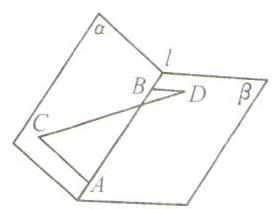
\includegraphics[width=0.2\textwidth]{bodyxb/src/bo_d20aucref24c73anc48g_158_1009_1247_272_209_0.jpg}
        \end{center}
        \begin{jieda}
            在平面 $\alpha$ 内,作 ${EB}\bot l$ 于 $B$ ,并取 ${EB} = {CA}$ ,连接 ${EC},{ED}$ ,则四边形 ${ACEB}$ 为矩形,且 $l \bot$ 平面 ${EBD},\angle {EBD}$ 就是二面角 $\alpha  - l - \beta$ 的平面角. $l \bot  {ED},l//{EC},\therefore {EC} \bot  {ED}$ . 在 $\bigtriangleup {EBD}$ 中使用余弦定理: $E{D}^{2} = B{E}^{2} + B{D}^{2} - 2 \cdot  {BE} \cdot  {BD} \cdot  \cos \angle {EBD}$ ; 在 Rt $\bigtriangleup {CED}$ 中,由勾股定理: ${CD} = \sqrt{E{C}^{2} + E{D}^{2}} =$  $\sqrt{A{B}^{2} + A{C}^{2} + B{D}^{2} - 2 \cdot  {AC} \cdot  {BD} \cdot  \cos \angle {EBD}} = 4$ . 
            
            \ps 一般地,若异面直线 ${AC}\text{ 、 }{BD}$ 的公垂线段为 ${AB} = d$ ,夹角为 $\theta$ ,线段 ${AC} = a$ ,线段 ${BD} = b$ ,则 ${CD} = \sqrt{{d}^{2} + {a}^{2} + {b}^{2} \pm  {2ab}\cos \theta }$ ,向量 $\vv{AC},\vv{BD}$ 夹角为 $\theta \left( {\pi  - \theta }\right)$ 时取负 (正) 号.
        \end{jieda}

    \end{enumerate}
\end{enumerate}

\begin{center}  \textbf{(B)} \end{center}
\begin{enumerate}
    \item 在四面体 ${ABCD}$ 中,已知棱 ${AC}$ 的长为 $\sqrt{2}$ ,其余各棱长都为 1,则二面角 $A - {CD} - B$ 的余弦值为\dotfill{(\kh{C})}
    \xx{$\dfrac{1}{3}$}{$\dfrac{\sqrt{2}}{3}$}{$\dfrac{\sqrt{3}}{3}$}{$\dfrac{1}{2}$}
    \begin{jieda}
        \begin{enumerate}
            \item 方法1

            根据三面角余弦定理可知$cos\angle{ADB} = cos\angle{ADC} \cdot cos\angle{CDB} + sin\angle{ADC} \cdot sin\angle{CDB} \cdot cos\theta$，带入$\angle{ADC} = \ang{90}, \angle{ADB} = \ang{60}, \angle{CDB} = \ang{60}$可知$cos\theta = \dfrac{\sqrt{3}}{3}$
            \item 方法2 

            取 ${CD},{CA}$ 的中点 $E,F$ ,连接 $\bigtriangleup {EFB}$ 三边. 由题意, $\bigtriangleup {CDA},\bigtriangleup {CBA}$ 是等腰直角三角形,公共斜边为 ${AC}$ ; $\bigtriangleup {ABD},\bigtriangleup {CBD}$ 是等边三角形. ${AD} \bot  {DC},{FE}//{AD},\therefore {FE} \bot  {DC}$ ,又 ${BE} \bot  {DC},\therefore \angle {FEB}$ 就是二面角 $A - {CD} -$  $B$ 的平面角. ${FE} = \dfrac{1}{2}{AD} = \dfrac{1}{2},{BE} = \dfrac{\sqrt{3}}{2},{BF} = \dfrac{\sqrt{2}}{2}$ ,在 $\bigtriangleup  {FEB}$ 中使用余弦定理,得: $\cos \angle {FEB} = \dfrac{F{E}^{2} + B{E}^{2} - F{B}^{2}}{2 \cdot  {FE} \cdot  {BE}} = \dfrac{\sqrt{3}}{3}$ .
        \end{enumerate}
        
    \end{jieda}
    
    \item 已知 $P$ 为锐二面角 $\alpha  - l - \beta$ 棱上的点, ${PQ} \subset  \alpha ,{PQ}$ 与 $l$ 成 ${45}^{ \circ  }$ 角,与 $\beta$ 成 ${30}^{ \circ  }$ 角 (如图),则二面角 $\alpha  - l - \beta$ 的平面角的度数是 \dotfill{(\kh{B})}
    
    \begin{center}
    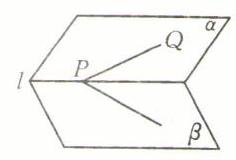
\includegraphics[width=0.2\textwidth]{bodyxb/src/bo_d20aucref24c73anc48g_158_1258_1979_236_160_0.jpg}
    \end{center}

    \xx{${30}^{ \circ  }$}{${45}^{ \circ  }$}{${60}^{ \circ  }$}{${75}^{ \circ  }$}
    \begin{jieda}
        记所求平面角为 $\theta  \in  \left( {0,\dfrac{\pi }{2}}\right)$ . 根据三正弦定理可知 $\sin \theta  \cdot  \sin {45}^{ \circ  } = \sin {30}^{ \circ  }$，$\therefore \theta  = {45}^{ \circ  }$
    \end{jieda}
    
    \item 如图,已知锐二面角 $\alpha  - l - \beta$ 的平面角为 $\theta ,m$ 是 $\alpha$ 内异于 $l$ 的一条直线,则 $m$ 与 $\beta$ 所成角的范围是\dotfill{(\kh{A})}   
    \begin{center}
    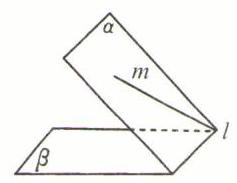
\includegraphics[width=0.2\textwidth]{bodyxb/src/bo_d20aucref24c73anc48g_159_422_363_237_183_0.jpg}
    \end{center}
    \xx{$\left\lbrack  {0,\theta }\right\rbrack$}{$\left\lbrack  {\theta ,\dfrac{\pi }{2}}\right\rbrack$}{$\left\lbrack  {\theta ,\pi  - \theta }\right\rbrack$}{$\left( {0,\dfrac{\pi }{2}}\right\rbrack$}
    \begin{jieda}
        记 $m$ 与 $\beta$ 所成角为 $\gamma .m$ 异于 $l$ 有两种情况: \ding{172} $m//l$ . 又 $l \subset  \beta ,\therefore m//\beta$ ,此时 $\gamma  = 0;\text{ \ding{173} }m$ 与 $l$ 相交,此时 $\gamma  \in$  $\left( {0,\dfrac{\pi }{2}}\right\rbrack$ ,记 $m$ 与 $l$ 所成锐角或直角为 $\delta  \in  \left( {0,\dfrac{\pi }{2}}\right\rbrack$ 
        
        根据三正弦定理, $\sin \theta \sin \delta  = \sin \gamma$ ,且 $\theta  \in  \left( {0,\dfrac{\pi }{2}}\right)$ ,故 $\sin \theta  \geq  \sin \gamma ,\therefore \gamma  \in  (0,\theta \rbrack$ (可以取遍这个区间内的任意值). 综上 $\gamma  \in  \left\lbrack  {0,\theta }\right\rbrack$ 
    \end{jieda}

    \item 如图,已知二面角 $\alpha  - l - \beta$ 的平面角为 $\theta$ ,在面 $\alpha$ 内有一条射线 ${AB}$ 与棱 $l$ 成锐角 $\delta$ ,与面 $\beta$ 成角 $\gamma$ ,则必有 \dotfill{(\kh{A})}
    
    \begin{center}
    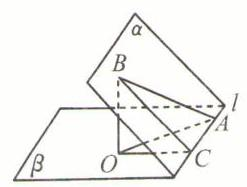
\includegraphics[width=0.2\textwidth]{bodyxb/src/bo_d20aucref24c73anc48g_159_819_355_247_187_0.jpg}
    \end{center}
    \xx{$\sin \theta \sin \delta  = \sin \gamma$}{$\sin \theta \sin \delta  = \cos \gamma$}{$\cos \theta \cos \delta  = \sin \gamma$}{$\cos \theta \cos \delta  = \cos \gamma$} 
    \begin{jieda}
        需分类讨论: $\text{ \ding{172} }\theta  \in  \left( {0,\dfrac{\pi }{2}}\right)$ . 记点 $B$ 在平面 $\beta$ 上的射影是点 $O$ ,作 ${OC}\bot l$ 于 $C$ ,连接 ${BC},{BO},{OA}.{BA}$ 在平面 $\beta$ 上的射影是 ${OA},\therefore \angle {BAO}$ 就是 ${AB}$ 与平面 $\beta$ 所成的角, $\sin \gamma  = \dfrac{BO}{BA}$ . 由三垂线定理, ${OC} \bot  l \Longrightarrow  {BC} \bot  l,\therefore \angle {BCO}$ 就是二面角 $\alpha  - l - \beta$ 的平面角, $\sin \theta  = \dfrac{BO}{BC},\sin \delta  = \dfrac{BC}{BA}$ . 此时, $\sin \theta \sin \delta  = \sin \gamma$ . \ding{173} $\theta  = \dfrac{\pi }{2}$ . 此时作 ${BC}\bot l$ 于 $C$ ,则有 ${BC}\bot$ 平面 $\beta$ ,即 $\angle {BAC}$ 就是 ${AB}$ 与平面 $\beta$ 所成的角, $\delta  = \gamma ,\sin \theta \sin \delta  = \sin \gamma$ 仍成立. \ding{174} $\theta  \in  \left( {\dfrac{\pi }{2},\pi }\right)$ . 和\ding{172}类似,记点 $B$ 在平面 $\beta$ 上的射影是点 $O$ (在半平面 $\beta$ 之外),作 ${OC} \bot  l$ 于 $C$ ,连接 ${BC}\text{ 、 }{BO}\text{ 、 }{OA}$ . 此时仍有 $\sin \gamma  = \sin \angle {BAO} = \dfrac{BO}{BA}$ 和 $\sin \delta  = \sin \angle {BAC} = \dfrac{BC}{BA}$ ,但 $\angle {BCO}$ 的补角才是二面角 $\alpha  - l - \beta$ 的平面角, $\sin \left( {\pi  - \theta }\right)  = \dfrac{BO}{BC} = \sin \theta ,\therefore \sin \theta \sin \delta  = \sin \gamma$ 仍成立. \ding{175}若允许 $\theta  =$ 0 或 $\theta  = \pi$ ,则平面 $\alpha \text{ 、 }\beta$ 共面,不论 $\delta  \in  \left( {0,\dfrac{\pi }{2}}\right)$ 取值为何,必有 $\gamma  = 0\left( {{AB}\text{ 在 }\beta \text{ 上 }}\right) ,\sin \theta \sin \delta  = \sin \gamma$ 仍成立. 综上, $\sin \theta \sin \delta  =$  $\sin \gamma$ 对任意 $\theta  \in  \left\lbrack  {0,\pi }\right\rbrack$ 和 $\delta  \in  \left( {0,\dfrac{\pi }{2}}\right)$ 均成立. 
        
        \ps $\delta$ 的范围可以拓展至 $\delta  \in  \left\lbrack  {0,\dfrac{\pi }{2}}\right\rbrack$ ,结论仍然成立.
    \end{jieda}
    \item 
    \begin{enumerate}
        \item 在正方体 ${ABCD} - {A}_{1}{B}_{1}{C}_{1}{D}_{1}$ 中,求二面角 $B - C{B}_{1} - A$ 的正弦值
        \begin{jieda}
            设正方体的边长为 1,所成二面角为 $\theta  \in  \left( {0,\dfrac{\pi }{2}}\right\rbrack$ . 取 $C{B}_{1}$ 的中点 $O$ ,连接 ${OB},{OA}$ . 在等腰直角三角形 $B{B}_{1}C$ 和等边三角形 $A{B}_{1}C$ 中, ${OB},{OA}$ 是底边上的中线,故 ${OB} \bot  C{B}_{1},{OA} \bot  C{B}_{1},\therefore \angle {BOA}$ 就是二面角 $B - C{B}_{1} -$  $A$ 的平面角. 又 ${AB} \bot$ 平面 ${BC}{C}_{1}{B}_{1},\therefore {AB} \bot  {BO},\tan \theta  = \dfrac{AB}{OB} = \sqrt{2},\therefore \sin \theta  = \dfrac{\sqrt{6}}{3}$
        \end{jieda}
        \item 已知 $E$ 是正方体 ${ABCD} - {A}_{1}{B}_{1}{C}_{1}{D}_{1}$ 的棱 ${BC}$ 的中点,求平面 ${B}_{1}{D}_{1}E$ 与面 $B{B}_{1}{C}_{1}C$ 所成锐二面角的正切值 (如图)
        \begin{center}
        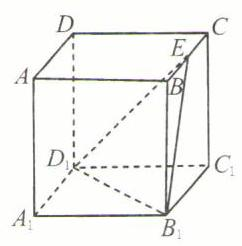
\includegraphics[width=0.2\textwidth]{bodyxb/src/bo_d20aucref24c73anc48g_159_409_1036_242_246_0.jpg}
        \end{center}
        \begin{jieda}
            设正方体的边长为 1,所成二面角为 $\theta  \in  \left( {0,\dfrac{\pi }{2}}\right\rbrack$ . 作 ${C}_{1}F \bot  E{B}_{1}$ 于点 $F$ ,则由 ${D}_{1}{C}_{1} \bot$ 面 $B{B}_{1}{C}_{1}C$ 知 ${D}_{1}F \bot$  $E{B}_{1}$ ,可算得所求角的正切值为 $\dfrac{\sqrt{5}}{2}$ . 注意: $\tan \theta  = \dfrac{{C}_{1}{D}_{1}}{{C}_{1}F}$ , ${C}_{1}F = \dfrac{{B}_{1}{C}_{1} \cdot  C{C}_{1}}{{B}_{1}E}$ (面积法).
        \end{jieda}
        \item 在棱长为 1 的正方体 ${ABCD} - {A}_{1}{B}_{1}{C}_{1}{D}_{1}$ 的棱 ${AB}$ 上求一点 $M$ ,使二面角 ${A}_{1} - M{B}_{1}$  $- C$ 的大小为 ${120}^{ \circ  }$ (如图)
        \begin{center}
        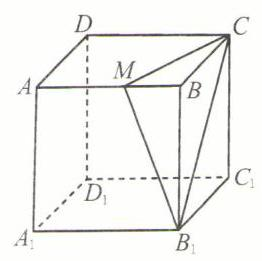
\includegraphics[width=0.2\textwidth]{bodyxb/src/bo_d20aucref24c73anc48g_159_910_1016_262_261_0.jpg}
        \end{center}
        \begin{jieda}
            作 ${BH}\bot M{B}_{1}$ 于点 $H$ ,则由 ${CB}\bot$ 面 ${A}_{1}{B}_{1}{BA}$ ,得 ${CH}\bot M{B}_{1}$，$\therefore \angle {CHB}$ 为二面角 $C - M{B}_{1} - B$ 的平面角,且 $\angle {CHB} = {60}^{ \circ  }$ . 令 ${MB} = x$ ,则可得 $x = \dfrac{\sqrt{2}}{2}$ ,即在棱 ${AB}$ 上取一点 $M$ , 使 ${MB} = \dfrac{\sqrt{2}}{2}$ . 注意: 由 $\bigtriangleup {BHM} \sim  \bigtriangleup {B}_{1}{BM}$ ,可得: $\dfrac{BH}{{B}_{1}B} = \dfrac{BM}{{B}_{1}M} \Longrightarrow  \dfrac{{BC} \cdot  \cot {60}^{ \circ  }}{{B}_{1}B} = \dfrac{x}{\sqrt{1 + {x}^{2}}},\therefore x = \dfrac{\sqrt{2}}{2}$ .
        \end{jieda}
    \end{enumerate}
    \item 在 ${60}^{ \circ  }$ 的二面角 $\alpha  - a  - \beta$ 内有一点 $P$ ,已知 ${PA} \bot  \alpha ,{PB} \bot  \beta ,A,B$ 为垂足,且 ${PA} = 3{{cm}}$ , ${PB} = 5{{cm}}$ ,求:
    \begin{enumerate*}
        \item $A,B$ 间的距离
        \item $P$ 到棱 $a$ 的距离
    \end{enumerate*}
    \begin{jieda}
        记平面 ${PAB}$ 与直线 $a$ 交于点 $C$ ,则 $a\bot$ 平面 ${PAB},\therefore a\bot {CA},a\bot {CB}$ .
        \begin{enumerate}
            \item $\angle {APB} = {180}^{ \circ  } - {60}^{ \circ  } = {120}^{ \circ  }$ ,在 $\bigtriangleup  {PAB}$ 中使用余弦定理，${AB} = \sqrt{P{A}^{2} + P{B}^{2} - 2 \cdot  {PA} \cdot  {PB} \cdot  \cos \angle {APB}} = 7{{cm}}.$
            \item $a \bot  {PC}$ ,故 ${PC}$ 即为所求. 四边形 ${PABC}$ 中, $\angle {PAC} = \angle {PBC} = {90}^{ \circ  }$ ,故四边形 ${PABC}$ 四点共圆,且 ${PC}$ 为直径. 在 $\bigtriangleup {PAB}$ 中使用正弦定理, ${PC} = \dfrac{AB}{\sin \angle {APB}} = \dfrac{14}{3}\sqrt{3}{{cm}}$ .
        \end{enumerate}
    \end{jieda}
    \item 在 ${120}^{ \circ  }$ 的二面角 $\alpha  - l - \beta$ 的面 $\alpha ,\beta$ 内分别有 $A,B$ 两点,且 $A,B$ 到棱 $l$ 的距离 ${AC},{BD}$ 分别是 $2,4,{AB} = {10}$ (如图),求:
    \begin{enumerate*}
        \item 直线 ${AB}$ 与棱 $l$ 所成角的正弦值
        \item 直线 ${AB}$ 与平面 $\beta$ 所成角的正弦值
    \end{enumerate*}
    \begin{center}
    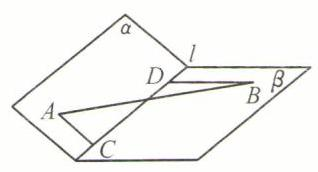
\includegraphics[width=0.2\textwidth]{bodyxb/src/bo_d20aucref24c73anc48g_159_337_1831_318_172_0.jpg}
    \end{center}
    \begin{jieda}
        \begin{enumerate}
            \item 在平面 $\beta$ 内,作 ${EC}\bot l$ 于 $C$ ,并取 ${EC} = {BD}$ ,连接 ${EA},{EB}$ ,则四边形 ${CEBD}$ 为矩形,且 $l\bot$ 平面 ${ACE},\angle {ACE}$ 就是二面角 $\alpha  - l - \beta$ 的平面角. 在 $\bigtriangleup {ACE}$ 中使用余弦定理: ${AE} = \sqrt{C{A}^{2} + C{E}^{2} - 2 \cdot  {CA} \cdot  {CE} \cdot  \cos \angle {ACE}} = 2\sqrt{7} \cdot  l \bot$  ${AE},l//{BE},\therefore {BE}\bot {AE}$ ,且直线 ${AB}$ 与棱 $l$ 所成角即 $\angle {ABE}.\sin \angle {ABE} = \dfrac{AE}{AB} = \dfrac{\sqrt{7}}{5}$ 
            \item 延长 ${EC}$ 至点 $F$ ,使得 ${CF} = {AC} \cdot  \sin {30}^{ \circ  } = 1$ ,连接 ${FA},{FB}$ . 此时 $l\bot {CA},l\bot {CF},\therefore l\bot$ 平面 ${CFA},\therefore l\bot$  ${FA}$ ；又由余弦定理, ${FA} = \sqrt{3},\therefore {FA}\bot {FC},\therefore {FA}\bot \beta ,\therefore \angle {ABF}$ 即为直线 ${AB}$ 与平面 $\beta$ 所成的角, $\sin \angle {ABF} = \dfrac{FA}{AB} = \dfrac{\sqrt{3}}{10}.$
        \end{enumerate}
    \end{jieda}
    \item 已知二面角 $\alpha  - {BC} - \beta$ 的大小为 ${120}^{ \circ  },A \in  \alpha ,D \in  \beta$ ,且 ${AB} \bot  {BC},{BC} \bot  {CD},{AB} = {BC} =$  ${CD} = 1$ (如图),求二面角 $A - {BD} - C$ 的平面角的正切值
    \begin{center}
    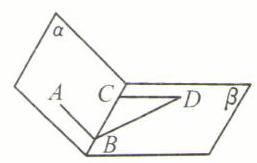
\includegraphics[width=0.2\textwidth]{bodyxb/src/bo_d20aucref24c73anc48g_159_915_1830_257_163_0.jpg}
    \end{center}
    \begin{jieda}
        过 $A$ 作 ${AH}\bot \beta$ 于 $H$ ,过 $H$ 作 ${DB}$ 的延长线的垂线, $E$ 为垂足,则 $\angle {AEH}$ 即为二面角 $A - {BD} - C$ 的平面角. 可算得 ${AH}$  $= \dfrac{\sqrt{3}}{2},{HE} = \dfrac{\sqrt{2}}{4},\tan \angle {AEH} = \sqrt{6}.$
    \end{jieda}
    \item 已知 ${PA},{PB},{PC}$ 是空间三条射线.
    \begin{enumerate}
        \item 若 $\angle {APB} = \angle {BPC} = \angle {CPA} = {60}^{ \circ  }$ ,求二面角 $B - {PA} - C$ 的平面角的正弦值
        \begin{jieda}
            根据三面角的余弦定理可知$cos\ang{60} = cos\ang{60} \cdot cos\ang{60} + sin\ang{60} \cdot sin\ang{60} \cdot cos\theta$，故$cos\theta = \dfrac{1}{3}$，即$sin\theta = \dfrac{2\sqrt{2}}{3}$
        \end{jieda}
        \item 若 $\angle {APC} = \angle {CPB} = {45}^{ \circ  },\angle {APB} = {60}^{ \circ  }$ ,求平面 ${APC}$ 与平面 ${BPC}$ 所成二面角的大小
        \begin{jieda}
            根据三面角的余弦定理可知$cos\ang{60} = cos\ang{45} \cdot cos\ang{45} + sin\ang{45} \cdot sin\ang{45} \cdot cos\theta$，故$cos\theta = 0$，即$\theta = \ang{90}$
        \end{jieda}
    \end{enumerate}
    \item 已知 $A,B$ 分别为二面角 $\alpha  - l - \beta$ 的面 $\alpha ,\beta$ 上的点,直线 ${AB}$ 与面 $\alpha ,\beta$ 分别成 ${\theta }_{1},{\theta }_{2}$ 角, $A$ , $B$ 在 $l$ 上的射影分别为点 $E,F$ (如图),求证: $\dfrac{BF}{AE} = \dfrac{\sin {\theta }_{1}}{\sin {\theta }_{2}}$ .
    
    \begin{center}
    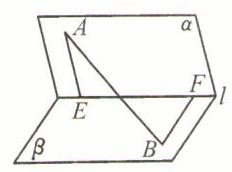
\includegraphics[width=0.2\textwidth]{bodyxb/src/bo_d20aucref24c73anc48g_160_275_575_232_172_0.jpg}
    \end{center}
    \begin{jieda}
        过 $A$ 作 ${AP}\bot \beta$ 于 $P$ ,过 $B$ 作 ${BQ}\bot \alpha$ 于 $Q$ ,则 $\sin {\theta }_{1} = \dfrac{BQ}{AB}$ , $\sin {\theta }_{2} = \dfrac{AP}{AB}$， $\angle{AEP} = \angle{BFQ} \Longrightarrow {{Rt}} \bigtriangleup  {APE}\sim {{Rt}} \bigtriangleup  {BQF} \Longrightarrow \dfrac{BQ}{AP} = \dfrac{BF}{AE}$ ,故 $\dfrac{BF}{AE} = \dfrac{\sin {\theta }_{1}}{\sin {\theta }_{2}}$
    \end{jieda}
    \item 已知二面角 $\alpha  - {MN} - \beta$ 的大小为 ${60}^{ \circ  },A \in  \alpha ,B \in  \beta ,{BC}$ 为 ${AB}$ 在 $\beta$ 上的射影,且 $C$ 在棱 ${MN}$ 上, ${AB}$ 与 $\beta$ 所成角为 ${60}^{ \circ  }$ ,且 ${AC} = \sqrt{5},\angle {MCB} = {45}^{ \circ  }$ (如图),求线段 ${AB}$ 的长
    
    \begin{center}
    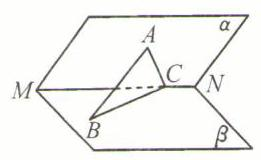
\includegraphics[width=0.2\textwidth]{bodyxb/src/bo_d20aucref24c73anc48g_160_635_586_261_160_0.jpg}
    \end{center}
    \begin{jieda}
        作 ${AO} \bot  \beta$ 交 ${BC}$ 于 $O$ ,再作 ${AD} \bot  {MN}$ 于 $D$ ,则 $\angle {ADO} = {60}^{ \circ  }$ ,记 ${AB} = a$ ,则 ${AD} = a$ , $\therefore {DC} = {OD} = \dfrac{a}{2}$ . 由 $A{D}^{2} + D{C}^{2} = A{C}^{2}$ ,可求得 ${AB} = a = 2$
    \end{jieda}

    \item 已知二面角 $\alpha  - {DC} - \beta$ 的度数为 $\theta ,A \in  \alpha ,B \in  \beta ,\bigtriangleup {ADC}$ 的面积为 $S$ ,且 ${DC} = m,{AB} \bot$  ${DC},{AB}$ 与平面 $\beta$ 成 ${30}^{ \circ  }$ 角 (如图),当 $\theta$ 变化时,求 $\bigtriangleup {DBC}$ 面积的最大值.
        
    \begin{center}
    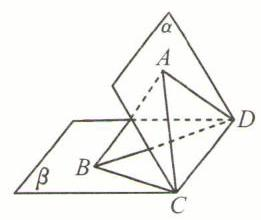
\includegraphics[width=0.2\textwidth]{bodyxb/src/bo_d20aucref24c73anc48g_160_1040_525_261_220_0.jpg}
    \end{center}
    \begin{jieda}
        过 $A$ 作 ${AH} \bot$ 面 $\beta$ 于 $H$ ,则 ${BH} \bot  {DC}$ ,垂足记为 $E$ . 于是在 $\bigtriangleup {ABE}$ 中,由 $\dfrac{BE}{\sin \left( {\theta  + {30}^{ \circ  }}\right) } = \dfrac{AE}{\sin {30}^{ \circ  }}$ ,得 ${BE} = {2AE} \cdot \sin \left( {\theta  + {30}^{ \circ  }}\right)  = \dfrac{4S}{m}\sin \left( {\theta  + {30}^{ \circ  }}\right)$ ,故当 $\theta  = {60}^{ \circ  }$ 时, $\bigtriangleup  {DBC}$ 面积的最大值为 ${2S}$ .

        \ps 确定了$\angle{ABE}$和$AE$这一组对边和对角，则外接圆半径是确定的，当且仅当$BE$为外接圆直径时取得最大值.$BE$取得最大值即$\bigtriangleup  {DBC}$ 面积取得最大值.
    \end{jieda}
    
    \item 已知二面角 $\alpha  - l - \beta$ 的大小为 ${30}^{ \circ  },l$ 上有两点 $A,B$ ,在半平面 $\alpha$ 内,过 $A,B$ 各作一条射线相交于点 $C$ ,使 $\angle {CAB} = {45}^{ \circ  }$ , $\angle {CBA} = {60}^{ \circ  }$ (如图).
    \begin{center}
    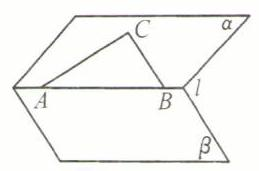
\includegraphics[width=0.2\textwidth]{bodyxb/src/bo_d20aucref24c73anc48g_160_452_1395_259_171_0.jpg}
    \end{center}
    \begin{enumerate}
        \item 求直线 ${AC},{BC}$ 与平面 $\beta$ 所成角的正弦值
        \begin{jieda}
            根据三正弦定理可知$sin\theta_1 = sin\ang{45} \cdot sin\ang{30} = \dfrac{\sqrt{2}}{4}$，$sin\theta_2 = sin\ang{60} \cdot sin\ang{30} = \dfrac{\sqrt{3}}{4}$
        \end{jieda}
        \item 若 ${AB} = 4$ ,求点 $C$ 到平面 $\beta$ 的距离
        \begin{jieda}
            做$CH \bot AB$，垂足为$H$，则$CH = \dfrac{4\sqrt{3}}{1+\sqrt{3}}$，做$CO \bot \beta$，垂足为$O$，则$CO = \dfrac{CH}{2} = \dfrac{2\sqrt{3}}{1+\sqrt{3}} = 3-\sqrt{3}$
        \end{jieda}
    \end{enumerate}
    \item 已知 $C$ 是以 ${AB}$ 为直径的圆周上一点, $\angle {ABC} = {30}^{ \circ  },{PA} \bot$ 平面 ${ABC},\angle {PBA} = {45}^{ \circ  }$ (如图),求二面角 $A - {PB} - C$ 的平面角的正弦值

    \begin{center}
    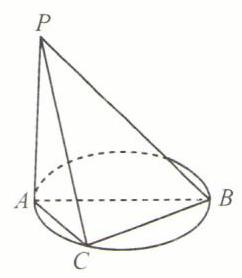
\includegraphics[width=0.2\textwidth]{bodyxb/src/bo_d20aucref24c73anc48g_160_905_1290_242_278_0.jpg}
    \end{center}
    \begin{jieda}
        过 $C$ 作 ${CE}\bot {AB}$ 于 $E$，因为${PA} \bot$ 平面 ${ABC}$，所以$CE \bot PA$，故${CE} \bot$ 平面 ${PAB}$
        
        过 $C$ 作 ${CD}\bot {PB}$ 于 $D$，连接$DE$，则$DE$是$CD$在平面$PAB$内射影，根据三垂线定理可知$PB \bot DE$，故$\angle {CDE}$ 是二面角 $A - {PB} - C$ 的平面角
        
        设 ${AB} = 2$，算得 ${CE} = \dfrac{\sqrt{3}}{2},{CD} = \dfrac{\sqrt{30}}{4},\therefore \sin \angle {CDE} = \dfrac{\sqrt{10}}{5}$
    \end{jieda}
    
    \item 二面角 $\alpha  - {PQ} - \beta$ 的大小为 ${60}^{ \circ  },A \in  \alpha ,B \in  \beta ,C \in  {PQ},\angle {ACP} = \angle {BCP} = {30}^{ \circ  },{CA} = {CB} = a$ (如图).
    
    \begin{center}
    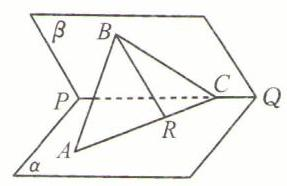
\includegraphics[width=0.2\textwidth]{bodyxb/src/bo_d20aucref24c73anc48g_160_1186_1873_287_186_0.jpg}
    \end{center}
    \begin{enumerate}
        \item 求证: ${AB}\bot {PQ}$
        \item 求点 $B$ 到平面 $\alpha$ 的距离
        \item 设 $R$ 是线段 ${CA}$ 上的点,直线 ${BR}$ 与平面 $\alpha$ 成 ${45}^{ \circ  }$ 角,求 ${CR}$ 的长
    \end{enumerate}
    \begin{jieda}
        \begin{enumerate}
            \item 做$AH \bot PQ$，交$PQ$于$H$，连接$BH$，因为$\left\{\begin{array}{l}
                 CA = CB \\
                 \angle {ACP} = \angle {BCP} \\
                 CH = CH
            \end{array}\right.$，所以$\triangle ACH \cong \triangle ABH$，故$BH \bot PQ$，故$PQ \bot $平面$ABH$，故$AB \bot PQ$
            \item 做$BO \bot \alpha$，交$\alpha$于$O$，计算可知$BH = \dfrac{a}{2}$，$BO = \dfrac{\sqrt{3}a}{4}$，即为点 $B$ 到平面 $\alpha$ 的距离.
            \item 因为直线 ${BR}$ 与平面 $\alpha$ 成 ${45}^{ \circ  }$ 角，所以$OR = BO$，计算可知$\dfrac{OR}{CH} = \dfrac{AO}{AH}$，故$R$为$AC$中点，$CR = \dfrac{a}{2}$
        \end{enumerate}
    \end{jieda}
    \item 已知二面角 $\alpha  - {MN} - \beta$ 的大小为 ${60}^{ \circ  },A \in  \alpha ,B \in  \beta ,C \in  {MN}$ ,且 $\angle {ACM} = \angle {BCN} = {45}^{ \circ  },{AC} = 1$ (如图),求:
    
    \begin{center}
    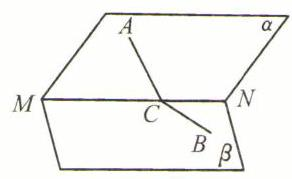
\includegraphics[width=0.2\textwidth]{bodyxb/src/bo_d20aucref24c73anc48g_161_1127_138_292_179_0.jpg}
    \end{center}

    \begin{enumerate}
        \item 点 $A$ 到平面 $\beta$ 的距离
        \item 二面角 $A - {BC} - M$ 的平面角的正切值
    \end{enumerate}
    \begin{jieda}
        \begin{enumerate}
            \item 作 ${AD} \bot$ 平面 $\beta$ 于 $D,{DE} \bot  {MN}$ 于 $E$ ,由三垂线定理, ${AE} \bot  {MN},\angle {AED}$ 即为二面角 $\alpha  - {MN} - \beta$ 的平面角. ${AD} = {AE} \cdot  \sin {60}^{ \circ  } = {AC} \cdot  \sin {45}^{ \circ  } \cdot  \sin {60}^{ \circ  } = \dfrac{\sqrt{6}}{4}$ ,即为所求.
            \item 做$AF \bot BC$，交$BC$于$F$，则$\angle{AFD}$即为二面角 $A - {BC} - M$ 的平面角. 

            \begin{center}
            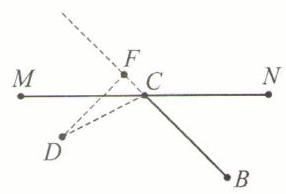
\includegraphics[width=0.2\textwidth]{bodyxb/src/bo_d20cdrf7aajc73bfmvhg_132_1227_247_286_194_0.jpg}
            \end{center}
            
            计算可得$DF = \dfrac{\sqrt{2}}{2}CE + \dfrac{\sqrt{2}}{2}DE = \dfrac{3}{4}$，故$tan\angle{AFD} = \dfrac{AD}{DF} = \dfrac{\sqrt{6}}{3}$
        \end{enumerate}
    \end{jieda}
    \item 在边长为$2$的正方体 ${ABCD} - {A}_{1}{B}_{1}{C}_{1}{D}_{1}$ 中,利用 $\cos \theta  = \dfrac{{S}_{\text{ 射影 }}}{S}$ 解下列各题:
    \begin{enumerate}
        \item $P,Q$ 分别为 ${A}_{1}A,{AB}$ 的中点,求平面 ${C}_{1}{PQ}$ 和底面 ${ABCD}$ 所成锐二面角的余弦值 (如图)
        \begin{center}
        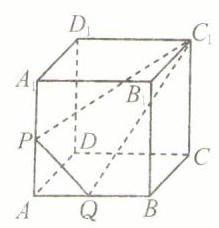
\includegraphics[width=0.2\textwidth]{bodyxb/src/bo_d20aucref24c73anc48g_161_282_709_219_228_0.jpg}
        \end{center}
        \begin{jieda}
            $\theta  \in  \left( {0,{90}^{ \circ  }}\right\rbrack  .\bigtriangleup {PQ}{C}_{1}$ 在平面 ${ABCD}$ 上的射影是 $\bigtriangleup {AQC}.{S}_{\bigtriangleup {AQC}} = \dfrac{1}{2} \cdot  {QA} \cdot  {CB} = 1;\bigtriangleup {PQ}{C}_{1}$ 中, ${C}_{1}Q = {C}_{1}P = 3$ , ${PQ} = \sqrt{2}$ ,底边 ${PQ}$ 上的高为 $h = \sqrt{{C}_{1}{Q}^{2} - {\left( \dfrac{PQ}{2}\right) }^{2}} = \dfrac{\sqrt{34}}{2},\therefore {S}_{\bigtriangleup {PQ}{C}_{1}} = \dfrac{1}{2} \cdot  {PQ} \cdot  h = \dfrac{\sqrt{17}}{2},\therefore \cos \theta  =$  $\dfrac{{S}_{\bigtriangleup {AQC}}}{{S}_{\bigtriangleup {PQ}{C}_{1}}} = \dfrac{2\sqrt{17}}{17}.$
        \end{jieda}
        \item 求二面角 ${C}_{1} - B{D}_{1} - C$ 的大小(如图)
        \begin{center}
        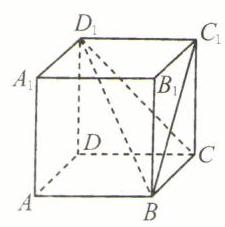
\includegraphics[width=0.2\textwidth]{bodyxb/src/bo_d20aucref24c73anc48g_161_629_707_225_227_0.jpg}
        \end{center}
        \begin{jieda}
            $\theta  \in  \left( {0,{90}^{ \circ  }}\right\rbrack$ . 连接 ${B}_{1}C$ 与 $B{C}_{1}$ 交于点 $E$ ,连接 $E{D}_{1}.{CE} \bot  B{C}_{1}\text{ 、 }{CE} \bot  {D}_{1}{C}_{1}$，$\therefore {CE} \bot$ 平面 $B{D}_{1}{C}_{1},\therefore \bigtriangleup {CB}{D}_{1}$ 在平面 ${C}_{1}B{D}_{1}$ 上的射影是 $\bigtriangleup {EB}{D}_{1},{S}_{\bigtriangleup {CB}{D}_{1}} = \dfrac{1}{2} \cdot  {CB} \cdot  C{D}_{1} = 2\sqrt{2}$ , ${S}_{\bigtriangleup {EB}{D}_{1}} = \dfrac{1}{2} \cdot  {EB} \cdot  {D}_{1}{C}_{1} = \sqrt{2},\therefore \cos \theta  = \dfrac{{S}_{\bigtriangleup {EB}{D}_{1}}}{{S}_{\bigtriangleup {CB}{D}_{1}}} = \dfrac{1}{2},\theta  = {60}^{ \circ  }$ .
        \end{jieda}
        \item $M$ 是棱 ${BC}$ 的中点(如图),求二面角 ${D}_{1} - {B}_{1}M - {C}_{1}$ 的平面角的余弦值
        \begin{center}
        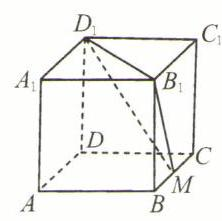
\includegraphics[width=0.2\textwidth]{bodyxb/src/bo_d20aucref24c73anc48g_161_982_712_222_221_0.jpg}
        \end{center}
        \begin{jieda}
            $\theta  \in  \left( {0,{90}^{ \circ  }}\right\rbrack  .\bigtriangleup {D}_{1}{B}_{1}M$ 在平面 ${B}_{1}M{C}_{1}$ 上的射影是 $\bigtriangleup {C}_{1}{B}_{1}M.\bigtriangleup {D}_{1}{B}_{1}M$ 中, ${B}_{1}{D}_{1} = 2\sqrt{2},{B}_{1}M = \sqrt{5},{D}_{1}M = 3$ ,

            $\therefore \cos \angle {D}_{1}{B}_{1}M = \dfrac{{B}_{1}{D}_{1}^{2} + {B}_{1}{M}^{2} - {D}_{1}{M}^{2}}{2 \cdot  {B}_{1}{D}_{1} \cdot  {B}_{1}M} = \dfrac{\sqrt{10}}{10}$ ,
            
            $\therefore {S}_{\bigtriangleup {D}_{1}{B}_{1}M} = \dfrac{1}{2} \cdot  {B}_{1}{D}_{1} \cdot  {B}_{1}M \cdot  \sin \angle {D}_{1}{B}_{1}M = 3;{S}_{\bigtriangleup {C}_{1}{B}_{1}M} = \dfrac{1}{2} \cdot  {C}_{1}{B}_{1} \cdot  {C}_{1}C = 2,\therefore \cos \theta  = \dfrac{{S}_{\bigtriangleup {C}_{1}{B}_{1}M}}{{S}_{\bigtriangleup {D}_{1}{B}_{1}M}}$  $= \dfrac{2}{3}$ .
        \end{jieda}
    \end{enumerate}
    \item 已知 $D,E$ 分别是边长为 $a$ 的等边三角形 ${ABC}$ 边 ${AB},{AC}$ 上的点, ${DE}//{BC}$ . 现沿 ${DE}$ 将 $\bigtriangleup {ADE}$ 折起,使二面角 $A - {DE} - B$ 成 ${60}^{ \circ  }$ 角 (如图). 当 ${DE}$ 在什么位置时,使折起后的顶点 $A$ 到 ${BC}$ 边的距离最短? 最短距离是多少?
    
    \begin{center}
    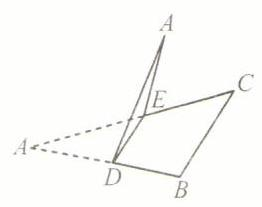
\includegraphics[width=0.2\textwidth]{bodyxb/src/bo_d20aucref24c73anc48g_161_289_1245_262_207_0.jpg}
    \end{center}
    \begin{jieda}
        取$DE$中点$F$，$BC$中点$G$，设$AF = x$，则$FG = \dfrac{\sqrt{3}a}{2} - x$，易知$AG$在平面$DECB$内的射影为$FG$根据三垂线定理可知$BC \bot AG$，故$AG$即为$A$ 到 ${BC}$ 边的距离.
        在$\triangle AFG$中根据余弦定理有$AG^2 = x^2 + \left(\dfrac{\sqrt{3}a}{2} - x\right)^2 - x \cdot \left(\dfrac{\sqrt{3}a}{2} - x\right)$，当且仅当$x = \dfrac{\sqrt{3}a}{4}$时取得最小值，此时有$AG = \dfrac{\sqrt{3}}{4}a$.
    \end{jieda}
    
    \item 等腰直角三角形 ${ABC}$ 和 ${{Rt}} \bigtriangleup  {DBC}$ 有公共边 ${BC},\angle {BAC} = \angle {BCD} = {90}^{ \circ  },\angle {BDC} = {60}^{ \circ  }$ (如图甲). 以 ${BC}$ 为棱折成多少度的二面角时 (如图乙),有 ${AD} = {CD}$ ?
    \begin{center}
    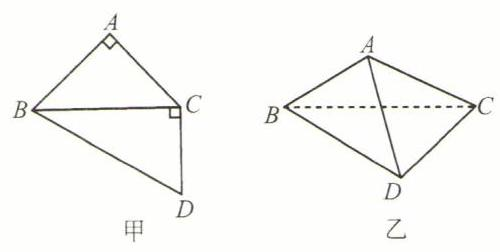
\includegraphics[width=0.4\textwidth]{bodyxb/src/bo_d20aucref24c73anc48g_161_711_1197_500_252_0.jpg}
    \end{center}
    \begin{jieda}
        设$CD = 2\sqrt{6}$，则$AC = 6$，$AD = \sqrt{24 + 18 - 2 \times 2\sqrt{6} \times 3\sqrt{2} \times cos\theta} = 2\sqrt{6}$，故$cos\theta = \dfrac{\sqrt{3}}{2}$，即$\theta = \ang{30}$
    \end{jieda}
    
    \item $E,F$ 分别是正方形 ${ABCD}$ 的边 ${AB},{CD}$ 的中点 (如图甲). 以 ${EF}$ 为棱,将正方形所在平面折成 ${120}^{ \circ  }$ 的二面角 (如图乙), $G$ 是棱 ${EF}$ 上一点,且满足 $\angle {AGF} = \angle {AGB}$ ,求:
    
    \begin{center}
    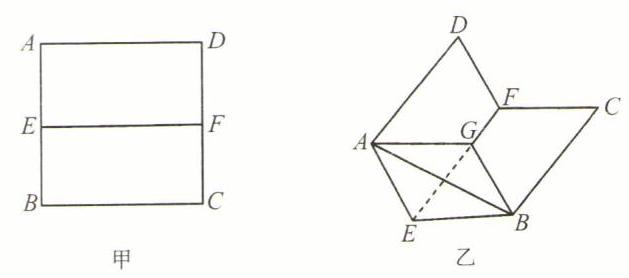
\includegraphics[width=0.5\textwidth]{bodyxb/src/bo_d20aucref24c73anc48g_161_780_1647_629_278_0.jpg}
    \end{center}
    \begin{enumerate}
        \item ${AG}$ 和平面 ${BCFE}$ 所成角的正弦值
        \item 二面角 $A - {BG} - E$ 的大小
    \end{enumerate}
    \begin{jieda}
        \begin{enumerate}
            \item 根据三面角的余弦定理可知$cos\angle{AGB} = cos\angle{AGE} \cdot cos\angle{BGE} + sin\angle{AGE} \cdot sin\angle{BGE} \cdot cos\angle{AEB}$

            根据$\angle {AGF} = \angle {AGB}$可知$cos\angle{AGB} = -cos\angle{AGE}$，正方形的对称性可知$\angle{AGE} = \angle{BGE}$

            设$c = cos\angle{AGE}$，则有$-c = c^2+(1-c^2)\cdot\left(-\dfrac{1}{2}\right)$，解得$c = \dfrac{1}{3}$或$-1$（舍）

            做$AH \bot EB$于$H$，连接$GH$，易知$\angle{AGH}$即为${AG}$ 和平面 ${BCFE}$ 所成角.根据三正弦定理可知$sin\angle{AGH} = sin\angle{AEB} \times sin\angle{AGE} = \dfrac{\sqrt{3}}{2} \times \dfrac{2\sqrt{2}}{3} = \dfrac{\sqrt{6}}{3}$
            \item 做$HM \bot BG$于$M$，则$\angle{AMH}$即为所求，根据三正弦定理$sin \angle{AMH} \times sin\angle{ABG} = sin \angle{ABH}$，$cos2\angle{ABG} = -cos\angle{AGB} = \dfrac{1}{3}$，故$sin\angle{ABG} = \dfrac{\sqrt{3}}{3}$，又因为$\angle{ABH} = \ang{30}$，所以$sin \angle{AMH} = \dfrac{\sqrt{3}}{2}$，根据题意可知二面角 $A - {BG} - E$ 的大小为$\ang{60}$
        \end{enumerate}
    \end{jieda}
\end{enumerate}

\subsection*{(三)两个平面垂直}

\subsubsection*{【典型题型和解题技巧】}

1. 两个平面垂直的证明

(1)利用两个平面互相垂直的定义.

如果两个平面相交,它们所成的二面角是直二面角,就说这两个平面互相垂直.

\textbf{例 1} 已知菱形 ${ABCD}$ 的边长为 ${2a},\angle {BAD} = {60}^{ \circ  },{AE},{CF}$ 都垂直于平面 ${ABCD}$ ,且 ${AE}$  $= {3a},{CF} = a,E,F$ 在平面 ${ABCD}$ 的同侧 (如图),求证: 平面 ${EBD} \bot$ 平面 ${FBD}$ .

\begin{center}
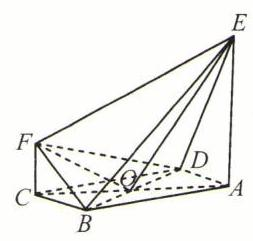
\includegraphics[width=0.2\textwidth]{bodyxb/src/bo_d20aucref24c73anc48g_162_1236_661_253_241_0.jpg}
\end{center}

\textbf{证明} 

连接 ${AC}$ ,交 ${BD}$ 于点 $O$ ,则 $O$ 为 ${AC},{BD}$ 的中点. 显然, ${EB} = {ED},{FB} = {FD}$ ,于是 ${EO}\bot {BD},{FO}\bot {BD}$，$\therefore \angle {EOF}$ 是二面角 $E - {BD} - F$ 的平面角.

$\because {AB} = {2a},\angle {BAD} = {60}^{ \circ  }$，$\therefore {AO} = {CO} = \sqrt{3}a$ ,而 ${AE} = {3a},{CF} = a$ ,则 $E{O}^{2} = A{O}^{2} + A{E}^{2} =$

${12}{a}^{2},F{O}^{2} = C{O}^{2} + C{F}^{2} = 4{a}^{2},E{O}^{2} + F{O}^{2} = {16}{a}^{2}.$

又 $\because E{F}^{2} = {\left( AE - CF\right) }^{2} + A{C}^{2} = 4{a}^{2} + {12}{a}^{2} = {16}{a}^{2}$ ,

$\therefore \angle {EOF} = {90}^{ \circ  }$ ,即二面角 $E - {BD} - F$ 是直二面角,故平面 ${EBD} \bot$ 平面 ${FBD}$ .

(2)利用两个平面垂直的判定定理:如果一个平面经过另一个平面的一条垂线,那么这两个平面互相垂直. 可记为

$\left. \begin{array}{l} \text{ 直线 }l \bot  \text{ 平面 }\alpha , \\  \text{ 直线 }l \subset  \text{ 平面 }\beta , \end{array}\right\}   \Longrightarrow  \alpha  \bot  \beta .$

\textbf{例 2} 已知 ${PA} \bot$ 圆 $O$ 所在平面, ${AB}$ 是圆 $O$ 的直径, $C$ 为圆周上一点 (如图),在四面体 ${PABC}$ 中:
\begin{center}
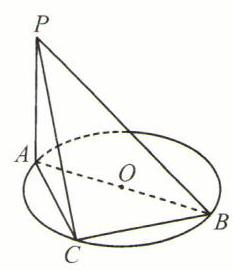
\includegraphics[width=0.2\textwidth]{bodyxb/src/bo_d20aucref24c73anc48g_162_1276_1458_233_270_0.jpg}
\end{center}

(1)有几个直角三角形？证明你的结论；

(2)有几对平面互相垂直？证明你的结论.

\textbf{解}

(1)有四个直角三角形: ${{Rt}} \bigtriangleup  {PAB},{{Rt}} \bigtriangleup  {PAC},{{Rt}} \bigtriangleup  {ACB}$ 和 ${{Rt}} \bigtriangleup  {PCB}$ .

$\because {PA} \bot$ 平面 ${ABC}$ ,

$\therefore {PA} \bot  {AB},{PA} \bot  {AC},\bigtriangleup {PAB}$ 和 $\bigtriangleup {PAC}$ 是直角三角形.

又 $\because {AB}$ 是圆 $O$ 直径,

$\therefore {BC} \bot  {AC}$ ,而 ${AC}$ 是 ${PC}$ 在面 ${ABC}$ 上的射影,

$\therefore {BC} \bot  {PC}$ ,故 $\bigtriangleup {ACB}$ 和 $\bigtriangleup {PCB}$ 也是直角三角形.

(2)有三对互相垂直的平面:平面 ${PAB} \bot$ 平面 ${ABC}$ ,平面 ${PAC} \bot$ 平面 ${ABC}$ ,平面 ${PBC} \bot$ 平面 ${PAC}$.

$\because {PA} \bot$ 平面 ${ABC},{PA} \subset$ 平面 ${PAB},\therefore$ 平面 ${PAB} \bot$ 平面 ${ABC}$ .

同理,平面 ${PAC} \bot$ 平面 ${ABC}$ .

又 $\because {PA} \bot$ 平面 ${ABC},\therefore {PA} \bot  {BC}$ ,而 ${AC} \bot  {BC},{PA} \cap  {AC} = A$ ,

$\therefore {BC} \bot$ 平面 ${PAC}.\because {BC} \subset$ 平面 ${PBC},\therefore$ 平面 ${PBC} \bot$ 平面 ${PAC}$ .

2. 两个平面垂直的性质.

(1)利用两个平面垂直的定义, 如果两个平面互相垂直, 那么它们的平面角是直角.

(2)利用两个平面垂直的性质定理,如果两个平面互相垂直,那么在一个平面上垂直于交线的直线垂直于另一个平面. 可记为

$\left. \begin{array}{l} \text{ 平面 }\alpha  \bot  \text{ 平面 }\beta , \\  \text{ 平面 }\alpha  \cap  \text{ 平面 }\beta  = l, \\  \text{ 直线 }a \subset  \alpha , \\  a \bot  l, \end{array}\right\}   \Longrightarrow  a \bot  \beta .$

\textbf{例 3} 已知 ${AB}$ 是夹在直二面角 $\alpha  - l - \beta$ 之间的一条线段,且 ${AB}$ 与 $\alpha ,\beta$ 分别成 ${45}^{ \circ  }$ 和 ${30}^{ \circ  }$ 的角, ${AB} = a$，求 ${AB}$ 在 $l$ 上的射影长及 ${AB}$ 和 $l$ 所成角的大小.

\begin{center}
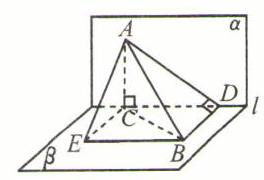
\includegraphics[width=0.2\textwidth]{bodyxb/src/bo_d20aucref24c73anc48g_163_1179_794_264_180_0.jpg}
\end{center}

\textbf{解} 

在 $\alpha$ 内作 ${AC} \bot  l$ 于点 $C$ ,在 $\beta$ 内 ${BD} \bot  l$ 于点 $D$. $\because \alpha  \bot  \beta ,\therefore {AC} \bot  \beta ,{BD} \bot  \alpha$ .

连接 ${BC},{AD}$ ,则 $\angle {ABC} = {30}^{ \circ  },\angle {BAD} = {45}^{ \circ  }.\because {AB} = a$ ,

$\therefore {AC} = \dfrac{a}{2},{AD} = \dfrac{\sqrt{2}}{2}a$ ,于是, ${CD} = \sqrt{A{D}^{2} - A{C}^{2}} = \dfrac{a}{2}$ ,即 ${AB}$ 在 $l$ 上的射影长等于 $\dfrac{a}{2}$ .

在 $\beta$ 内过点 $B$ 作 $l$ 的平行线,过点 $C$ 作 ${DB}$ 的平行线,两线交于点 $E$ ,则 $\angle {ABE}$ 就是 ${AB}$ 与 $l$ 所成的角或其补角. 连接 ${AE}$ ,由 ${BE} \bot  {CE}$ 知, ${BE} \bot  {AE}$ (三垂线定理).

在 ${{Rt}} \bigtriangleup  {AEB}$ 中, $\cos \angle {ABE} = \dfrac{BE}{AB} = \dfrac{\dfrac{a}{2}}{a} = \dfrac{1}{2},\therefore \angle {ABE} = {60}^{ \circ  }$ ,即 ${AB}$ 与 $l$ 成 ${60}^{ \circ  }$ 角.

(3)利用两个平面垂直性质定理的推论,如果两个平面互相垂直,那么经过第一个平面上一点且垂直于第二个平面的直线必在第一个平面上. 可记为

$\left. \begin{array}{l} \text{ 平面 }\alpha  \bot  \text{ 平面 }\beta , \\  \text{ 点 }P \in  \alpha , \\  P \in  \text{ 直线 }l, \\  l \bot  \beta , \end{array}\right\}   \Longrightarrow  l \subset  \alpha .$

\textbf{例 4} 如果两个相交平面都和第三个平面垂直, 那么它们的交线也和第三个平面垂直.

已知: 平面 $\alpha  \cap$ 平面 $\beta  = l,\alpha  \bot$ 平面 $\gamma ,\beta  \bot  \gamma$ ,求证: $l \bot  \gamma$ .

\threetu{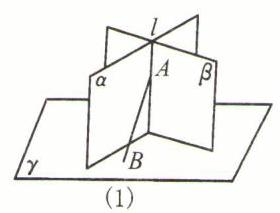
\includegraphics[width=0.6\textwidth]{bodyxb/src/bo_d20aucref24c73anc48g_164_295_151_280_213_0.jpg}}{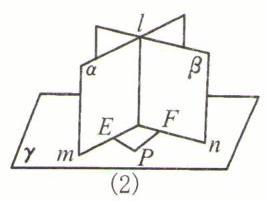
\includegraphics[width=0.6\textwidth]{bodyxb/src/bo_d20aucref24c73anc48g_164_704_167_267_201_0.jpg}}{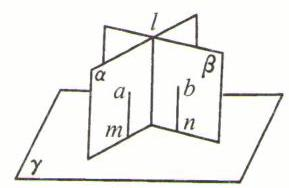
\includegraphics[width=0.6\textwidth]{bodyxb/src/bo_d20aucref24c73anc48g_164_1096_150_289_188_0.jpg}}

\textbf{证法一} 

在 $l$ 上任取一点 $A$ ,作 ${AB} \bot  \gamma$ [如图(1)].

$\because \alpha  \bot  \gamma ,\therefore {AB} \subset  \alpha$ (两个平面垂直性质定理的推论). 同理, ${AB} \subset  \beta$ ,故 ${AB} = \alpha  \cap  \beta$ .

而 $\alpha  \cap  \beta  = l,\therefore {AB}$ 与 $l$ 重合, $\therefore l \bot  \gamma$ .


\textbf{证法二} 

设 $\alpha  \cap  \gamma  = m,\beta  \cap  \gamma  = n$ ,在 $\gamma$ 内取一点 $P$ ,并在 $\gamma$ 内作 ${PE} \bot  m,{PF} \bot  n\lbrack E,F$ 为垂足, [如图(2)].

$\because \gamma  \bot  \alpha ,\therefore {PE} \bot  \alpha$ (两个平面垂直的性质定理),于是 ${PE} \bot  l$ .

同理 ${PF} \bot  l$ ,而 ${PE} \cap  {PF} = P,\therefore l \bot  \gamma$ .

\textbf{证法三} 

记 $\alpha  \cap  \gamma  = m,\beta  \cap  \gamma  = n$ ,分别在 $\alpha ,\beta$ 内作 $a \bot  m,b \bot  n$ [如图(3)].

$\because \alpha  \bot  \gamma ,\beta  \bot  \gamma ,\therefore a \bot  \gamma ,b \bot  \gamma$ (两个平面垂直的性质定理),于是 $a//b$ .

又 $\because a \not \subset \beta ,b \subset  \beta ,\therefore a//\beta$ . 而 $a \subset  \alpha ,\alpha  \cap  \beta  = l,\therefore a//l$ . 于是由 $a\bot \gamma$ ,得 $l\bot \gamma$ .

\subsubsection*{【训练题】}

\begin{center}  \textbf{(A)} \end{center}
\begin{enumerate}
    \item 已知平面 $\alpha  \bot$ 平面 $\beta ,\alpha  \cap  \beta  = l$ ,点 $P \in  l$ ,给出以下四个结论: \ding{172}过点 $P$ 和 $l$ 垂直的直线在 $\alpha$ 内；\ding{173}过点 $P$ 和 $\beta$ 垂直的直线在 $\alpha$ 内；\ding{174}过点 $P$ 和 $l$ 垂直的直线也和 $\beta$ 垂直；\ding{175}过点 $P$ 和 $\beta$ 垂直的平面也和 $l$ 垂直. 其中正确的个数是 \dotfill{(\kh{A})}
    \xx{1}{2}{3}{4}
    \begin{jieda}
        根据两个平面垂直性质定理的推论,\ding{173}正确. 其余结论的反例如下: 在正方体 ${ABCD} - {A}_{1}{B}_{1}{C}_{1}{D}_{1}$ 中,取 $\alpha  =$ 平面 ${AD}{D}_{1}{A}_{1},\beta  =$ 平面 ${ADCB},l = {AD}$ ,点 $P =$ 点 $A$ ,对于\ding{172}\ding{174},取直线为 $A{B}_{1}$ ; 对于\ding{175},取平面为 ${AC}{C}_{1}{A}_{1}$
    \end{jieda}
    \item 下列命题正确的是\dotfill{(\kh{C})}
    \xx{过平面外一点作与这个平面垂直的平面是唯一的}{过直线外一点作这条直线的垂线是唯一的}{过平面的一条斜线作与这个平面垂直的平面是唯一的}{过直线外一点作与这条直线平行的平面是唯一的}
    \begin{jieda}
        对于选项 A,这样的平面有无数个,其作法为:过该点作已知平面的垂线 $l$ ,则任意过直线 $l$ 的平面均符合要求 (两个平面垂直的判定定理),而符合要求的平面也一定过直线 $l$ (两个平面垂直性质定理的推论); 对于选项 $B$ ,在平面几何中,该命题为真,但在立体几何中则有无数条; 对于选项 $C$ ,记平面 $\alpha$ 的一条斜线为 $l,l$ 在 $\alpha$ 上的射影是 ${l}^{\prime }$ ,则由相交直线 $l,{l}^{\prime }$ 确定的平面即为所求,其唯一性证明如下: (反证法),若平面 $\beta ,\gamma$ 都经过 $l$ ,又与平面 $\alpha$ 垂直, $\because l = \beta  \cap  \gamma ,\therefore$  $l\bot \alpha$ (见本节例 4),矛盾; 对于选项 $D$ ,这样的平面有无数个,其作法为:过该点作已知直线的平行线 $l$ ,则任意过 $l$ (但不过该点)的平面均符合要求,而符合要求的平面也一定过 $l$
    \end{jieda}
    \item 已知 $a,b$ 是平面 $\alpha$ 外的两条平行直线,则下列说法正确的是\dotfill{(\kh{A})}
    \xx{若 $a\bot \alpha ,b \subset$ 平面 $\beta$ ,则 $\alpha \bot \beta$}{若 $a$ 与 $c$ 是一对异面直线,且 $c \subset  \alpha$ ,则 $b$ 与 $\alpha$ 一定不平行}{若 ${b}^{\prime }$ 是 $b$ 在 $\alpha$ 上的射影,则 $a//{b}^{\prime }$}{若 ${a}^{\prime },{b}^{\prime }$ 分别是 $a,b$ 在 $\alpha$ 上的射影,则 ${a}^{\prime }//{b}^{\prime }$}
    \begin{jieda}
    选项 (A) 正确,证明如下: $a//b,a\bot \alpha ,\therefore b\bot \alpha$ ,又 $b \subset  \beta$ ,由两个平面垂直的判定定理, $\alpha \bot \beta$ ; 选项 (B) 错误, 反例: 在正方体 ${ABCD} - {A}_{1}{B}_{1}{C}_{1}{D}_{1}$ 中,取 $\alpha  =$ 平面 ${ABCD},a = {A}_{1}{B}_{1},b = {C}_{1}{D}_{1},c = {AD}$ ,则 $b//\alpha$ ; 选项 (C) 错误; 选项 (D) 错误,遗漏了 ${a}^{\prime }$ 与 ${b}^{\prime }$ 重合的可能性.
    \end{jieda}
    \item 若三个不同平面 $\alpha ,\beta ,\gamma$ 满足 $\alpha  \bot  \gamma ,\beta  \bot  \gamma$ ,则 $\alpha$ 与 $\beta$ 间的位置关系是 \dotfill{(\kh{D})}
    \xx{$\alpha //\beta$}{$\alpha  \bot  \beta$}{$\alpha //\beta$ 或 $\alpha \bot \beta$}{$\alpha //\beta$ 或 $\alpha$ 与 $\beta$ 相交}
    \begin{jieda}
        在正方体 ${ABCD} - {A}_{1}{B}_{1}{C}_{1}{D}_{1}$ 中,取 $\gamma  =$ 平面 ${ABCD},\alpha  =$ 平面 ${AD}{D}_{1}{A}_{1}$ ,当 $\beta  =$ 平面 ${BC}{C}_{1}{B}_{1}$ 时, $\alpha //\beta$ ;当 $\beta  =$ 平面 ${AC}{C}_{1}{A}_{1}$ 时, $\alpha$ 与 $\beta$ 相交但不互相垂直; 当 $\beta  =$ 平面 ${AB}{B}_{1}{A}_{1}$ 时, $\alpha  \bot  \beta$ . 故 $\alpha //\beta$ 或 $\alpha$ 与 $\beta$ 相交均有可能.
    \end{jieda}
    
    \item 沿对角线 ${AC}$ 将正方形 ${ABCD}$ 折成直二面角后, ${AB}$ 与 ${CD}$ 所在直线所成的角为\dotfill{(\kh{B})}
    \xx{${90}^{ \circ  }$}{${60}^{ \circ  }$}{${45}^{ \circ  }$}{${30}^{ \circ  }$}
    \begin{jieda}
        设折叠前$B$的位置为$B'$，$\angle{BAB'}$即为异面直线所成角，计算可知$AB = AB' = BB'$，故$\angle{BAB'} = \ang{60}$
    \end{jieda}
    \item 
    \begin{enumerate}
        \item 已知 ${PA} \bot$ 菱形 ${ABCD}$ 所在的平面 (如图),求证: 平面 ${PAC} \bot$ 平面 ${PBD}$
        \begin{center}
        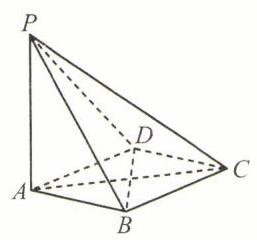
\includegraphics[width=0.2\textwidth]{bodyxb/src/bo_d20aucref24c73anc48g_165_454_329_257_240_0.jpg}
        \end{center}
        \begin{jieda}
            ${BD} \bot  {AC}$ , ${BD} \bot  {AP}$ ,又 ${AC} \cap  {AP} = A,\therefore {BD} \bot$ 平面 ${PAC}$ . 又 ${BD} \subset$ 平面 ${PBD}$ ,由两个平面垂直的判定定理, $\therefore$ 平面 ${PAC} \bot$ 平面 ${PBD}$ ,证毕.
        \end{jieda}
        \item 已知 $P$ 是菱形 ${ABCD}$ 所在平面外一点,且 ${PD} = {PB}$ (如图),求证: 平面 ${PAC} \bot$ 平面 ${PBD}$ 
        \begin{center}
        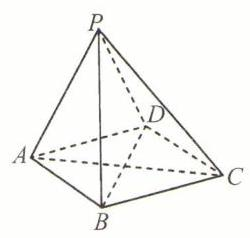
\includegraphics[width=0.2\textwidth]{bodyxb/src/bo_d20aucref24c73anc48g_165_839_329_250_238_0.jpg}
        \end{center}
        \begin{jieda}
            记 ${AC} \cap  {BD} = O$ ,连接 ${PO}.O$ 是等腰三角形 ${PBD}$ 底边 ${BD}$ 的中点, $\therefore {BD}\bot {PO}$ ,又 ${BD}\bot {AC}$ , ${AC} \cap  {PO} = O$ , $\therefore {BD} \bot$ 平面 ${PAC}$ . 又 ${BD} \subset$ 平面 ${PBD}$ ,由两个平面垂直的判定定理, $\therefore$ 平面 ${PAC} \bot$ 平面 ${PBD}$ ,证毕.
        \end{jieda}
    \end{enumerate}
    \item 已知 $P$ 是 $\bigtriangleup {ABC}$ 所在平面外一点, ${PA} = {PB} = {PC},\angle {BAC} = {90}^{ \circ  }$ (如图). 求证: 平面 ${PBC} \bot$ 平面 ${ABC}$ .
    
    \begin{center}
    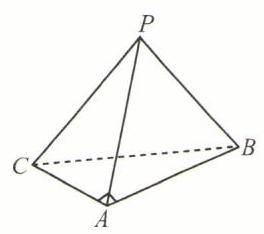
\includegraphics[width=0.2\textwidth]{bodyxb/src/bo_d20aucref24c73anc48g_165_261_778_264_234_0.jpg}
    \end{center}
    \begin{jieda}
        取 ${BC}$ 中点 $O$ ,则 ${AO} = {BO} = {CO},{PO}\bot {BC}$ . 再由 $P{O}^{2} + O{A}^{2} = P{O}^{2} + O{C}^{2} = P{C}^{2} = P{A}^{2}$ 得 ${PO}\bot {OA}$ , $\therefore {PO}\bot$ 平面 ${ABC}$ ,又 ${PO} \subset$ 平面 ${PBC},\therefore$ 平面 ${PBC} \bot$ 平面 ${ABC}$
    \end{jieda}

    \item \begin{enumerate}
        \item 已知 ${AB}\bot$ 平面 $\alpha$ 于 $B,{DC} \subset  \alpha$ ,且 ${DC}\bot {AC}$ 于点 $C$ (如图),求证: 平面 ${ACD}\bot$ 平面 ${ABC}$
        \begin{center}
        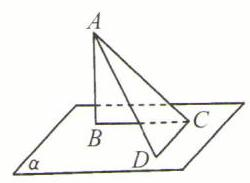
\includegraphics[width=0.2\textwidth]{bodyxb/src/bo_d20aucref24c73anc48g_165_652_826_250_183_0.jpg}
        \end{center}
        \begin{jieda}
            ${AB}\bot \alpha  \Longrightarrow  {DC}\bot {AB}$ ,又 ${DC}\bot {AC},{AB} \cap  {AC} = A$ , $\therefore {DC}\bot$ 平面 ${ABC}$ ,而 ${DC} \subset$ 平面 ${ACD}$ , $\therefore$ 平面 ${ACD}\bot$ 平面 ${ABC}$ ,证毕.
        \end{jieda}
        \item 已知平面 ${ABC} \bot$ 平面 ${ACD},{AB} \bot$ 平面 ${BCD}$ (如图),求证: ${CD}\bot {BC}$
        \begin{center}
        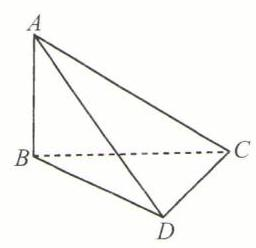
\includegraphics[width=0.2\textwidth]{bodyxb/src/bo_d20aucref24c73anc48g_165_1030_757_256_248_0.jpg}
        \end{center} 
        \begin{jieda}
            利用如下结论:若两个相交平面同时垂直于第三个平面,则这两个相交平面的交线与第三个平面垂直(见本节例 4). $\because {AB} \bot$ 平面 ${BCD}\text{ 、 }{AB} \subset$ 平面 ${ABC}$ ,
            
            $\therefore$ 平面 ${BCD} \bot$ 平面 ${ABC}$ . 又,平面 ${ACD} \bot$ 平面 ${ABC}$ ,而平面 ${BCD} \cap$ 平面 ${ACD} = {CD},\therefore {CD} \bot$ 平面 ${ABC}$，$\therefore {CD} \bot  {BC}$ ,证毕.
        \end{jieda}
    \end{enumerate}
    \item 等腰三角形 ${ABC}$ 的底 ${BC} = 4\sqrt{2}$ ,高 ${AD} = 1$ ,现沿 ${AD}$ 将 $\bigtriangleup {ABD}$ 折起,使二面角 $B - {AD} - C$ 为 ${60}^{ \circ  }$ (如图),求此时 ${AB}$ 与面 ${ACD}$ 所成角的正弦值
    
    \begin{center}
    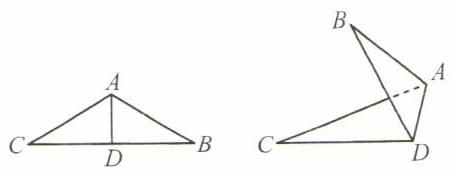
\includegraphics[width=0.3\textwidth]{bodyxb/src/bo_d20aucref24c73anc48g_165_980_1145_456_174_0.jpg}
    \end{center}
    \begin{jieda}
        折叠后,作 ${BE} \bot  {CD}$ 于 $E$ ,连接 ${AE}.\because {DB} \bot  {AD}\text{ 、 }{DC} \bot  {AD},\therefore {AD} \bot$ 平面 ${BDC}$ ,且 $\angle {BDC}$ 就是二面角 $B - {AD}$  $- C$ 的平面角, $\therefore  \bigtriangleup  {BDC}$ 是等边三角形, ${BE} = \dfrac{\sqrt{3}}{2} \cdot  {BD} = \sqrt{6}$ . 又, ${AD} \bot$ 平面 ${BDC},{AD} \subset$ 平面 ${ADC},\therefore$ 平面 ${BDC} \bot$ 平面 ${ADC}.{BE} \bot  {CD},\therefore {BE} \bot$ 平面 ${ADC},\therefore \angle {BAE}$ 就是 ${AB}$ 与平面 ${ACD}$ 所成的角, $\sin \angle {BAE} = \dfrac{BE}{AB}$  $= \dfrac{\sqrt{6}}{3}$ .
    \end{jieda}
\end{enumerate}

\begin{center}  \textbf{(B)} \end{center}
\begin{enumerate}
    \item 已知矩形 ${ADEF}$ 所在平面$\bot$矩形 ${BCEF}$ 所在平面,记 $\angle {DBE} = \alpha$ , $\angle {DCE} = \beta ,\angle {BDC} = \theta$ (如图),则下列各式成立的是\dotfill{(\kh{A})}
    
    \begin{center}
    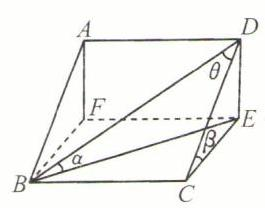
\includegraphics[width=0.2\textwidth]{bodyxb/src/bo_d20aucref24c73anc48g_165_1170_1551_265_208_0.jpg}
    \end{center}

    \xx{$\sin \alpha  = \sin \beta  \cdot  \cos \theta$}{$\sin \beta  = \sin \alpha  \cdot  \cos \theta$}{$\cos \alpha  = \cos \beta  \cdot  \cos \theta$}{$\cos \beta  = \cos \alpha  \cdot  \cos \theta$}
    \begin{jieda}
        三正弦定理.
    \end{jieda}
    
    \item 在直二面角 $\alpha  - l - \beta$ 的棱 $l$ 上取一点 $A$ ,过点 $A$ 分别在 $\alpha ,\beta$ 内点 $A$ 的同侧作与 $l$ 成 ${45}^{ \circ  }$ 角的射线,则这两射线所夹的角为\dotfill{(\kh{B})}
    \xx{${45}^{ \circ  }$}{${60}^{ \circ  }$}{${90}^{ \circ  }$}{${120}^{ \circ  }$}
    \begin{jieda}
        三余弦定理.
    \end{jieda}
    \item $a,b$ 为两条互不垂直的异面直线,过 $a,b$ 分别作平面 $\alpha ,\beta$ ,那么给出以下四个结论: $\text{ \ding{172} }b//$  $\alpha$ ；\ding{173} $b\bot \alpha$ ；\ding{174} $\alpha //\beta$ ；\ding{175} $\alpha \bot \beta$ . 其中不可能出现的结论个数是\dotfill{(\kh{A})}
    \xx{1}{2}{3}{4}
    \begin{jieda}
        结论\ding{173}中,若 $b\bot \alpha$ ,又 $a \subset  \alpha \therefore b\bot a$ ,与题设矛盾,故\ding{173}不可能成立. 其他 3 个结论均有可能,举例如下:在正方体 ${ABCD} - {A}^{\prime }{B}^{\prime }{C}^{\prime }{D}^{\prime }$ 中,取 $a = {AB},b = C{D}^{\prime }$ ,结论\ding{172}可取 $\alpha  = {AB}{B}^{\prime }{A}^{\prime }$ ; 结论\ding{174}可取 $\alpha  = {AB}{B}^{\prime }{A}^{\prime }$ 及 $\beta  = {CD}{D}^{\prime }{C}^{\prime }$ ; 结论 \ding{175} 可取 $\alpha  = {ABCD}$ 及 $\beta  = {CD}{D}^{\prime }{C}^{\prime }$ 
    \end{jieda}
    \item 一条线段的两个端点分别在一个直二面角的两个面内, 则这条线段与这两平面所成角的和一定\dotfill{(\kh{C})}
    \xx{等于 ${90}^{ \circ  }$}{大于 ${90}^{ \circ  }$}{不大于 ${90}^{ \circ  }$}{不小于 ${90}^{ \circ  }$}
    \begin{jieda}
        如图,线段 ${AB}$ 的端点 $A,B$ 分别在直二面角 $\alpha  - l - \beta$ 的半平面 $\alpha ,\beta$ 上. 作 ${AC} \bot  l$ 交 $l$ 于点 $C,{BD} \bot  l$ 交 $l$ 于点 $D$ ,连接 ${AD},{BC}$ ,则 ${AC} \bot  \beta ,{BD} \bot  \alpha ,{AB}$ 与平面 $\alpha ,\beta$ 所成的角分别为 $\angle {BAD},\angle {ABC}.\angle {BAD} + \angle {ABC} = \left( {\angle {ABC} - \angle {DBA}}\right)  + {90}^{ \circ  }.\sin \angle {ABC} =$  $\dfrac{AC}{AB} \leq  \dfrac{AD}{AB} = \sin \angle {DBA} \Longrightarrow  \angle {ABC} \leq  \angle {DBA} \Longrightarrow  \angle {BAD} + \angle {ABC} \leq  {90}^{ \circ  }$ (当且仅当 ${AC} = {AD}$ , 即 ${AB} \bot  l$ 时等号成立).
        
        \begin{center}
        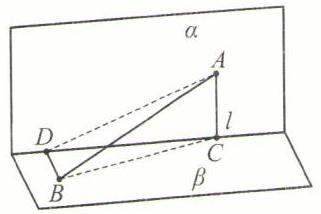
\includegraphics[width=0.2\textwidth]{bodyxb/src/bo_d20cdrf7aajc73bfmvhg_134_1211_1069_321_214_0.jpg}
        \end{center}
    \end{jieda}
    \item 在空间四边形 ${ABCD}$ 中,已知 ${AB} = {BC} = {CD} = {DA},M,N,P,Q,K$ 分别是 ${DC},{CB}$ , ${AB},{AD},{BD}$ 的中点 (如图),求证: 平面 ${KAC} \bot$ 平面 ${PQMN}$ .
    
    \begin{center}
    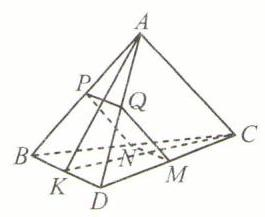
\includegraphics[width=0.2\textwidth]{bodyxb/src/bo_d20aucref24c73anc48g_166_316_511_265_217_0.jpg}
    \end{center}
    \begin{jieda}
        由 ${AK} \bot  {BD},{CK} \bot  {BD},{PQ}//{BD}//{MN}$ ,得 ${MN} \bot$ 平面 ${KAC}$ . 且 ${MN} \subset$ 平面 ${PQMN}$，$\therefore$ 平面 ${KAC} \bot$ 平面 ${PQMN}$
    \end{jieda}
    \item 在矩形 ${ABCD}$ 中,已知 ${AB} = {2AD},E$ 为 ${AB}$ 的中点 (如图甲). 将 $\bigtriangleup {ADE}$ 沿 ${DE}$ 折起,使折后 ${A}^{\prime }B = {A}^{\prime }C$ (如图乙),求证: 平面 ${A}^{\prime }{DE} \bot$ 平面 ${BCDE}$ 
    \begin{center}
    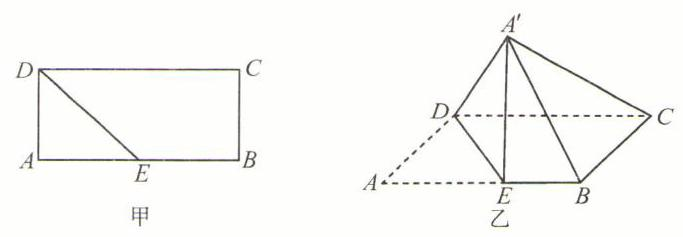
\includegraphics[width=0.5\textwidth]{bodyxb/src/bo_d20aucref24c73anc48g_166_683_494_683_237_0.jpg}
    \end{center}
    \begin{jieda}
        取$DE$中点$M$和$BC$中点$N$，因为${A}^{\prime }B = {A}^{\prime }C$，所以$AN \bot BC$，又因为$MN // AB$，所以$MN \bot BC$，因此$BC \bot $平面$A'MN$，故$BC \bot AM$，又有$AM \bot DE$，显然$BC \cap DE \neq \varnothing$，所以$AM \bot $平面 ${BCDE}$，因为$AM \subset $平面 ${A}^{\prime }{DE}$，所以平面 ${A}^{\prime }{DE} \bot$ 平面 ${BCDE}$ 
    \end{jieda}
    \item 在正方体 ${ABCD} - {A}_{1}{B}_{1}{C}_{1}{D}_{1}$ 中,已知 $P,Q,R,S$ 分别为棱 ${A}_{1}{D}_{1},{A}_{1}{B}_{1},{AB},B{B}_{1}$ 的中点 (如图),求证: 平面 ${PQS} \bot$ 平面 ${B}_{1}{RC}$ .
    
    \begin{center}
    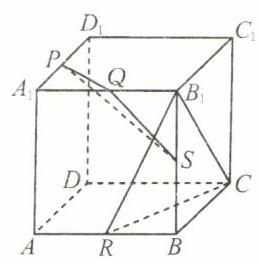
\includegraphics[width=0.2\textwidth]{bodyxb/src/bo_d20aucref24c73anc48g_166_309_1047_260_264_0.jpg}
    \end{center}
    \begin{jieda}
        取$AD$中点$P'$，则$BP'$是$PS$在面$ABCD$的射影，又因为$BP' \bot CR$，根据三垂线定理可知$CR \bot PS$

        取$B_1C_1$中点$P''$，则$P''S$是$PS$在面$BCC_1B_1$的射影，又因为$P''S \bot CB_1$，根据三垂线定理可知$CB_1 \bot PS$

        因此$PS \bot$平面$CRB_1$，故平面 ${PQS} \bot$ 平面 ${B}_{1}{RC}$
    \end{jieda}
    \item 已知 ${PA} \bot$ 矩形 ${ABCD}$ 所在的平面, $M,N$ 分别为 ${AB},{PC}$ 的中点 (如图).
    \begin{center}
    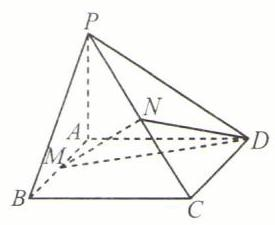
\includegraphics[width=0.2\textwidth]{bodyxb/src/bo_d20aucref24c73anc48g_166_700_1085_275_225_0.jpg}
    \end{center}
    \begin{enumerate}
        \item 求证: ${MN}\bot {AB}$
        \item 若平面 ${PDC}$ 与平面 ${ABCD}$ 成 ${45}^{ \circ  }$ 角,求证:平面 ${MND} \bot$ 平面 ${PDC}$ 
    \end{enumerate}
    \begin{jieda}
        \begin{enumerate}
            \item 取$AC$中点$Q$，则$NQ // PA$，因此$NQ \bot $平面$ABCD$，即$Q$为$N$在平面$ABCD$内的射影，因为$M,Q$分别为$AB, AC$的中点，所以$MQ // AD$，所以$MQ \bot AB$，故根据三垂线定理可知$AB \bot $平面$MNQ$，故$AB \bot MN$
            \item 因为$MN \bot AB$，所以$MN \bot CD$

            $\angle{PDA}$即为二面角$P-CD-A$的平面角，故$\angle{PDA} = \ang{45}$，设$PA = 2$，计算可得$MC = \sqrt{5}, NC = \sqrt{3}, MN = \sqrt{2}$，因此$MN \bot NC$

            所以$MN \bot $平面 ${PDC}$，故平面 ${MND} \bot$ 平面 ${PDC}$.
        \end{enumerate}
    \end{jieda}
    \item 在边长为 $a$ 的菱形 ${ABCD}$ 中, $\angle {ABC} = {120}^{ \circ  }$ ,线段 ${PC} \bot$ 面 ${ABCD}$ ,且 ${PC} = a,E$ 为 ${PA}$ 的中点 (如图)
    \begin{center}
    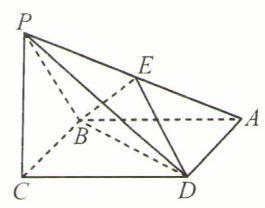
\includegraphics[width=0.2\textwidth]{bodyxb/src/bo_d20aucref24c73anc48g_166_1104_1103_265_208_0.jpg}
    \end{center}
    \begin{enumerate}
        \item 求证:平面 ${EBD}\bot$ 平面 ${ABCD}$
        \item 求二面角 $A - {BE} - D$ 的正切值
    \end{enumerate}
    \begin{jieda}
        \begin{enumerate}
            \item 记 ${AC} \cap  {BD} = O$ ,可证 ${OE} \bot$ 面 ${ABCD}$ ,从而平面 ${EBD} \bot$ 平面 ${ABCD}$
            \item 由$(1)$可知平面 ${EBD}\bot$ 平面 ${ABCD}$，又因为$AO \bot BD$，因此$AO \bot $面$EBD$，故$A$在面$EBD$内的射影为$O$，做$OF \bot BE$于$F$，则$\angle{AFO}$为二面角 $A - {BE} - D$的平面角

            计算可知$OE = \dfrac{a}{2}, BO = \dfrac{a}{2}$，因此$\triangle BOE$为等腰直角三角形，故$F$为$BE$中点，$OF = \dfrac{\sqrt{2}a}{4}$，$AO = \dfrac{\sqrt{3}a}{2}$，故$tan\angle{AFO} = \dfrac{AO}{OF} = \sqrt{6}$.
        \end{enumerate}
    \end{jieda}
    \item 
    \begin{enumerate}
        \item 线段 ${AB}$ 的两端在直二面角 $\alpha  - {CD} - \beta$ 的两个面内,并且与这两个面都成 ${30}^{ \circ  }$ 角 (如图),求异面直线 ${AB}$ 与 ${CD}$ 所成的角
        \begin{center}
        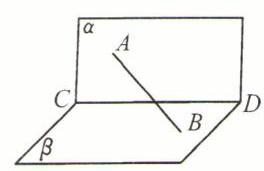
\includegraphics[width=0.2\textwidth]{bodyxb/src/bo_d20aucref24c73anc48g_166_1248_1907_264_171_0.jpg}
        \end{center}
        \begin{jieda}
            过$B$做直线$BP // CD$，使得$AP \bot CD$，故$\angle{ABP}$即为异面直线所成角.过$A$做$AQ \bot CD$，交$CD$于$Q$，故$\angle{ABQ} = \ang{30}$
            
            设$AQ = a$，则$AB = 2a, BQ = \sqrt{3}a$，过$B$做$BQ' \bot CD$交$CD$于$Q'$，则$\angle{BAQ'} = \ang{30}$，$BQ' = a$，故$BP = QQ' = \sqrt{2}a$，$PQ = BQ' = a$，故$AP = \sqrt{2}a$，因此$\angle{ABP} = \ang{45}$
        \end{jieda}
        \item 夹在直二面角两个半平面之间的一条线段与这两个半平面所成的角分别为 ${30}^{ \circ  },{45}^{ \circ  }$ ,若这条线段的长为 $a$ ,求它在二面角棱上的射影长
        \begin{jieda}
            借用$(1)$的图，则$AQ = \dfrac{a}{2}, BQ' = \dfrac{\sqrt{2}a}{2}$，$QQ' = \sqrt{a^2 - \left(\dfrac{a}{2}\right)^2-\left(\dfrac{\sqrt{2}a}{2}\right)^2} = \dfrac{a}{2}$
        \end{jieda}
        \item 夹在直二面角 $\alpha  - l - \beta$ 间的线段 ${AB}$ 和两个半平面 $\alpha ,\beta$ 分别成 ${30}^{ \circ  }$ 和 ${45}^{ \circ  }$ 角,若 $A,B$ 在 $l$ 上的射影间的距离为 1,求 ${AB}$ 的长
        \begin{jieda}
            由$(2)$可知答案为2.
        \end{jieda}
    \end{enumerate}
    \item 已知等腰直角三角形 ${ABD}$ 和等腰直角三角形 ${CBD}$ 所在平面互相垂直,且 $\angle {ADB} =$  $\angle {DBC} = {90}^{ \circ  }$ (如图),在 ${AB}$ 上取一点 $P$ ,当 $P$ 在什么位置时,二面角 $P - {CD} - B$ 的大小为 ${60}^{ \circ  }$ ?
    \begin{center}
    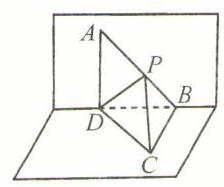
\includegraphics[width=0.2\textwidth]{bodyxb/src/bo_d20aucref24c73anc48g_167_461_431_224_187_0.jpg}
    \end{center}
    \begin{jieda}
        过$P$做$PQ \bot BD$，交$DB$于$Q$，则$Q$为$P$在面$BDC$内的射影，过$Q$做$QR \bot CD$，交$CD$于$R$，则$\angle{PRQ}$即为二面角 $P - {CD} - B$ 的平面角.

        设$BQ = k \cdot BD$，则$PQ = k \cdot BD$，$QR = \dfrac{1-k}{\sqrt{2}} \cdot BD$，若$\angle{PRQ} = \ang{60}$，则$PQ = \sqrt{3}QR$，即$k = \sqrt{3}\times \dfrac{1-k}{\sqrt{2}}$，因此$k = 3-\sqrt{6}$，故$BP = (3-\sqrt{6})AB$时满足要求.
    \end{jieda}
    \item 已知两个全等的正方形 ${ABCD}$ 和 ${CDEF}$ 所在平面互相垂直 (如图).

    \begin{center}
    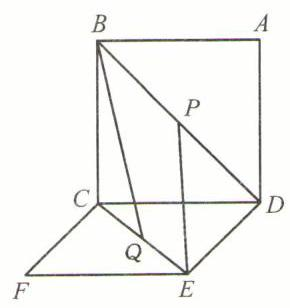
\includegraphics[width=0.2\textwidth]{bodyxb/src/bo_d20aucref24c73anc48g_167_792_310_290_308_0.jpg}
    \end{center}
    \begin{enumerate}
        \item 求 ${BD}$ 与 ${EC}$ 所成的角
        \item 若 $P,Q$ 分别为两个正方形的中心,求 ${BQ}$ 与 ${EP}$ 所成角的余弦值
    \end{enumerate}
    \begin{jieda}
        不妨设正方形边长为 1 .
        \begin{enumerate}
            \item 延长 ${FE}$ 至 $G$ ,使得 ${EG} = {FE}$ ,连接 ${GD},{GB}$ . 不难证明,四边形 ${CEGD}$ 是平行四边形, $\therefore {EC}//{GD},\angle {BDG}$ (或其补角) 就是 ${BD}$ 与 ${EC}$ 所成的角. ${DB} = {DG} = \sqrt{2},{BG} = \sqrt{B{C}^{2} + C{G}^{2}} = \sqrt{B{C}^{2} + C{F}^{2} + F{G}^{2}} = \sqrt{6}$ ,由余弦定理,得 $\cos \angle {BDG} = \dfrac{D{B}^{2} + D{G}^{2} - B{G}^{2}}{2 \cdot  {DB} \cdot  {DG}} =  - \dfrac{1}{2},\therefore \angle {BDG} = {120}^{ \circ  },\therefore {BD}$ 与 ${EC}$ 所成的角为 ${60}^{ \circ  }$ 
            \item 连接 ${BE}$ ,并取 ${BP}$ , ${BE}$ , ${QE}$ 三边中点 $K$ , $J$ , $Y$ ,连接 $\bigtriangleup {YJK}$ 的三边. 由三角形的中位线定理, $\angle {YJK}$ (或其补角)就是 ${BQ}$ 与 ${EP}$ 所成的角. ${JY} = \dfrac{1}{2}{BQ} = \dfrac{1}{2}\sqrt{B{C}^{2} + C{Q}^{2}} = \dfrac{\sqrt{6}}{4} = {JK}$ . 为求 ${YK}$ ,可由点 $K$ , $Y$ 向 ${CD}$ 引垂线,记垂足为 $M,N$ ,则 $Y{K}^{2} = K{M}^{2} + M{Y}^{2} = K{M}^{2} + M{N}^{2} + N{Y}^{2} = {\left( \dfrac{3}{4}\right) }^{2} + {\left( \dfrac{1}{2}\right) }^{2} + {\left( \dfrac{3}{4}\right) }^{2} = \dfrac{11}{8}$ . 由余弦定理,得 $\cos \angle {YJK} =$  $\dfrac{J{Y}^{2} + J{K}^{2} - Y{K}^{2}}{2 \cdot  {JY} \cdot  {JK}} =  - \dfrac{5}{6}$ ,故 ${BQ}$ 与 ${EP}$ 所成的角为 $\pi  - \angle {YJK}$ ,其余弦值为 $\cos \left( {\pi  - \angle {YJK}}\right)  =  - \cos \angle {YJK} = \dfrac{5}{6}$
        \end{enumerate}
    \end{jieda}
    \item 在平面四边形 ${ABCD}$ 中,已知 ${AB} = {BC} = {CD} = a,\angle {ABC} = {90}^{ \circ  },\angle {BCD} = {135}^{ \circ  }$ (如图甲). 沿 ${AC}$ 将四边形折成直二面角 $B - {AC} - D$ (如图乙).
    \begin{center}
    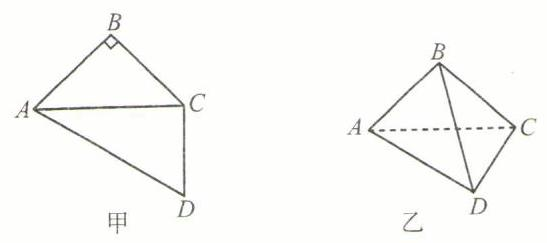
\includegraphics[width=0.4\textwidth]{bodyxb/src/bo_d20aucref24c73anc48g_167_254_1097_547_243_0.jpg}
    \end{center}
    \begin{enumerate}
        \item 求证: ${AB}\bot$ 平面 ${BCD}$
        \item 求二面角 $B - {AD} - C$ 的大小
    \end{enumerate}
    \begin{jieda}
        \begin{enumerate}
            \item 由题意, $\angle {BAC} = \angle {BCA} = {45}^{ \circ  },\therefore \angle {ACD} = {90}^{ \circ  }$ 
    
            $\because$ 平面 ${ACD} \bot$ 平面 ${ACB},{DC} \bot  {AC},\therefore {DC} \bot$ 平面 ${ACB},\therefore {DC} \bot  {AB}$ . 又 ${AB} \bot  {BC},{BC} \cap  {DC} = C$ , $\therefore {AB} \bot$ 平面 ${BCD}$ ,证毕.
            \item 折叠后,作 ${BE}\bot {AC}$ 于点 $E$ ,作 ${EF}\bot {AD}$ 于点 $F$ ,连接 ${BF}$ . 易证: ${BE}\bot$ 平面 ${ACD}$ ,故 ${BF}$ 在平面 ${ACD}$ 上的射影是 ${EF}$ ,又 ${EF} \bot  {AD}$ ,由三垂线定理得 ${BF} \bot  {AD},\therefore \angle {BFE}$ 就是所求二面角的平面角. ${BE} = \dfrac{\sqrt{2}}{2}{AB} = \dfrac{\sqrt{2}}{2}a, \bigtriangleup  {EAF} \sim   \bigtriangleup  {DAC},\therefore \dfrac{EF}{DC} = \dfrac{EA}{DA}$ ,即 $\dfrac{EF}{a} = \dfrac{\dfrac{\sqrt{2}}{2}}{\sqrt{3}a}$ ,得 ${EF} = \dfrac{\sqrt{6}}{6}a.\therefore \tan \angle {BFE} = \dfrac{BE}{EF} = \sqrt{3}$ , $\therefore \angle {BFE} = {60}^{ \circ  }$ .
        \end{enumerate}
    \end{jieda}
    \item 正方形 ${ABCD}$ 的边长为 7,点 $M,N$ 分别在 ${AD},{BC}$ 上,且 ${MN}//{AB},{DM} = 3$ ,现将正方形沿 ${MN}$ 折成直二面角 (如图)
    \begin{center}
    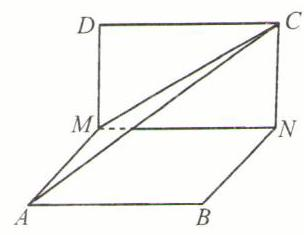
\includegraphics[width=0.2\textwidth]{bodyxb/src/bo_d20aucref24c73anc48g_167_963_1100_304_235_0.jpg}
    \end{center}
    \begin{enumerate}
        \item 求${AC}$ 与 ${MN}$ 所成角的正切值
        \item 求${AC}$ 与平面 ${MNCD}$ 所成角的正切值
    \end{enumerate}
    \begin{jieda}
        \begin{enumerate}
            \item 连接 ${CB}$ ,由题意, ${CN} \bot$ 平面 ${ABNM},\therefore {CN} \bot  {AB}$ ,又 ${BN} \bot  {AB},\therefore {AB} \bot$ 平面 ${CNB}$ . 由于 ${MN}//{AB},\therefore$  ${AC}$ 与 ${MN}$ 所成角即为 $\angle {CAB}$ 或其补角. 在 ${{Rt}} \bigtriangleup  {CAB}$ 中, $\angle {ABC} = {90}^{ \circ  },\tan \angle {CAB} = \dfrac{CB}{AB} = \dfrac{\sqrt{C{N}^{2} + N{B}^{2}}}{AB} = \dfrac{5}{7}$ .
            \item 由题意, ${AM} \bot$ 平面 ${MNCD}$ , $\therefore {AC}$ 在平面 ${MNCD}$ 上的射影是 ${MC}$ , $\therefore {AC}$ 与平面 ${MNCD}$ 所成角为 $\angle {ACM}.\tan \angle {ACM} = \dfrac{AM}{MC} = \dfrac{AM}{\sqrt{M{N}^{2} + M{D}^{2}}} = \dfrac{4}{\sqrt{{7}^{2} + {3}^{2}}} = \dfrac{2}{29}\sqrt{58}.$
        \end{enumerate}
    \end{jieda}
    \item 已知 $A,B$ 分别为直二面角 $\alpha  - l - \beta$ 的面 $\alpha ,\beta$ 内的点,且 ${AB}$ 的长为 $2,{AB}$ 与 $\alpha$ 成 ${45}^{ \circ  }$ 角, 与 $\beta$ 成 ${30}^{ \circ  }$ 角,作 ${AC} \bot  l$ 于点 $C,{BD} \bot  l$ 于点 $D$ (如图),求二面角 $C - {AB} - D$ 的余弦值.
    
    \begin{center}
    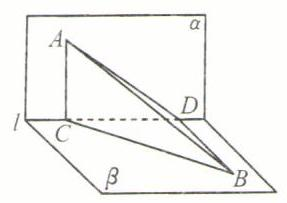
\includegraphics[width=0.2\textwidth]{bodyxb/src/bo_d20aucref24c73anc48g_167_628_1759_287_203_0.jpg}
    \end{center}
    \begin{jieda}
        由题意, ${AC} \bot  \beta ,{BD} \bot  \alpha$ , ${AB}$ 在平面 $\alpha ,\beta$ 内的射影分别为 ${AD},{CB}.\because {AB}$ 与平面 $\alpha ,\beta$ 所成的角分别为 $\angle {DAB} = {45}^{ \circ  }$ , $\angle {ABC} = {30}^{ \circ  },\therefore {AC} = 1,{BC} = \sqrt{3},{DA} = {DB} = \sqrt{2},{CD} = \sqrt{A{D}^{2} - A{C}^{2}} = 1$ . 作 ${DE} \bot  {BC}$ 于 $E,{EF} \bot  {AB}$ 于 $F$ ,连接 ${DF}.\because {DE} \bot  {BC},{DE} \bot  {AC},\therefore {DE} \bot$ 平面 ${ABC}$ ,又 ${EF} \bot  {AB}$ ,由三垂线定理, ${DF} \bot  {AB},\therefore \angle {EFD}$ 就是二面角 $C - {AB} - D$ 的平面角. ${DE} = \dfrac{{CD} \cdot  {DB}}{BC} = \dfrac{\sqrt{6}}{3},{DF} = \dfrac{{DA} \cdot  {DB}}{AB} = 1$，$\therefore \sin \angle {EFD} = \dfrac{DE}{DF} = \dfrac{\sqrt{6}}{3},\therefore \cos \angle {EFD} = \dfrac{\sqrt{3}}{3}$ .
    \end{jieda}
    \item 
    \begin{enumerate}
        \item 在 Rt $\bigtriangleup {ABC}$ 中,已知 $\angle {ACB} = {90}^{ \circ  },{AC} = 1,\angle A = {60}^{ \circ  },D$ 为 ${AB}$ 的中点 (如图甲),将 $\bigtriangleup {ABC}$ 沿中线 ${CD}$ 折成直二面角 $B - {CD} - A$ (如图乙),求:\ding{172}直线 ${AB}$ 与平面 ${ACD}$ 所成角的正切值,\ding{173}二面角 $B - {AC} - D$ 的正切值
        \begin{center}
        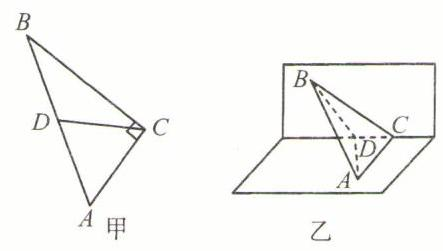
\includegraphics[width=0.3\textwidth]{bodyxb/src/bo_d20aucref24c73anc48g_168_385_249_443_251_0.jpg}
        \end{center}
        \begin{jieda}
            \begin{dingautolist}{172}
                \item 作 ${BE} \bot$ 直线 ${CD}$ 于点 $E$ , ${AF} \bot$ 直线 ${CD}$ 于点 $F$ ,连接 ${AE}$ . 由题意, ${BE} \bot$ 平面 ${ACD}$，$\therefore {AB}$ 在平面 ${ACD}$ 上的射影是 ${AE}$ ,直线 ${AB}$ 与平面 ${ACD}$ 所成的角是 $\angle {BAE}.{DA} = {DC} = {DB} = {AC} = 1,{BC} =$  $\sqrt{3},{BE} = {BC} \cdot  \sin \angle {BCE} = \dfrac{\sqrt{3}}{2},{AE} = \sqrt{A{F}^{2} + F{E}^{2}} = \sqrt{{\left( \dfrac{\sqrt{3}}{2}\right) }^{2} + {1}^{2}} = \dfrac{\sqrt{7}}{2},\therefore \tan \angle {BAE} = \dfrac{BE}{AE} = \dfrac{\sqrt{21}}{7}$ . 
                \item 作 ${EG} \bot  {AC}$ 于点 $G$ ,连接 ${BG}.{EG}$ 是 ${BG}$ 在平面 ${DCA}$ 上的射影,由三垂线定理, ${BG} \bot  {AC}$. $\therefore \angle {BGE}$ 就是二面角 $B - {AC} - D$ 的平面角. ${EG} = {EC} \cdot  \sin \angle {DCA} = \dfrac{3\sqrt{3}}{4},\therefore \tan \angle {BGE} = \dfrac{BE}{EG} = \dfrac{2}{3}$ .
            \end{dingautolist}
        \end{jieda}
        \item 已知 ${{Rt}} \bigtriangleup  {ABC}$ 的两直角边 ${AC} = 2,{BC} = 3,P$ 是斜边 ${AB}$ 上的点(如图甲),以 ${CP}$ 棱折成直二面角 $A - {CP} - B$ (如图乙),若折后 ${AB} = \sqrt{7}$ ,试求二面角 $P - {AC} - B$ 的余弦值
        \begin{center}
        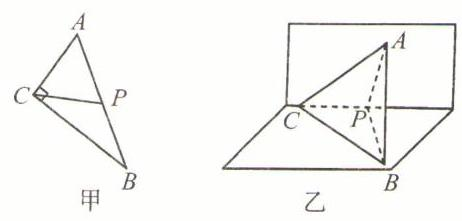
\includegraphics[width=0.3\textwidth]{bodyxb/src/bo_d20aucref24c73anc48g_168_988_279_462_221_0.jpg}
        \end{center}
        \begin{jieda}
            计算可知$cos\angle{ACB} = \dfrac{4+9-7}{2\times2\times3} = \dfrac{1}{2}$，根据三余弦定理可知$cos\angle{ACB} = cos\angle{ACP} \cdot cos\angle{BCP}$，又因为$\angle{BCP} + \angle{ACP} = \ang{90}$，故$\angle{ACP} = \angle{BCP} = \ang{45}$

            做$PQ \bot AC$于$Q$，做$QR \bot AC$交$BC$于$R$，故$\angle{PQR}$即为二面角 $P - {AC} - B$ 的平面角，计算可得$CR = 2, QR = \sqrt{3}, PQ = 1, PR = \sqrt{2}$，因此$cos\angle{PQR} = \dfrac{\sqrt{3}}{3}$.
        \end{jieda}
    \end{enumerate}
    \item \begin{enumerate}
        \item 已知平面 $\alpha  \bot$ 平面 $\beta ,l \subset  \alpha ,m \subset  \beta$ ,且 $l \bot  m$ (如图),求证: $l \bot  \beta$ 或 $m \bot  \alpha$
        \begin{center}
        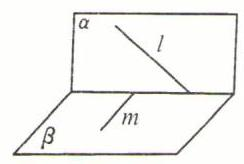
\includegraphics[width=0.2\textwidth]{bodyxb/src/bo_d20aucref24c73anc48g_168_332_1031_244_164_0.jpg}
        \end{center}
        \begin{jieda}
            设 $\alpha  \cap  \beta  = c$ ,若 $l\bot c$ ,则 $l\bot \beta$ ; 若 $l$ 与 $c$ 不垂直,则可过 $l$ 上一点 $P$ 作直线 $a$ ,使得 $a\bot c$ 交 $c$ 于点 $Q$ ,由 $\alpha \bot \beta$ ,可得 $a\bot \beta ,\therefore m\bot a$ ,再由 $m\bot l$ ,得 $m\bot \alpha$ .
        \end{jieda}
        \item 已知 $\alpha  \bot  \beta ,\alpha  \cap  \beta  = {AB},a \subset  \alpha ,b \subset  \beta ,a,b$ 与 ${AB}$ 都不垂直 (如图),求证: $a$ 与 $b$ 不垂直
        \begin{center}
        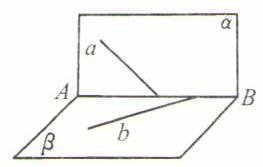
\includegraphics[width=0.2\textwidth]{bodyxb/src/bo_d20aucref24c73anc48g_168_704_1026_263_167_0.jpg}
        \end{center}
        \begin{jieda}
            若 $a\bot b$ ,由(1)知,有 $a\bot \beta$ 或 $b\bot \alpha$ ,从而 $a\bot {AB}$ 或 $b\bot {AB}$ ,和题设矛盾,故 $a$ 与 $b$ 不垂直,证毕.
        \end{jieda}
    \end{enumerate} 
    \item 已知定线段 ${AB} \bot$ 平面 $\alpha ,l$ 是平面 $\alpha$ 内不过点 $B$ 的一条定直线,过 ${AB}$ 的两个平面 $\beta ,\gamma$ 互相垂直,且分别与 $l$ 交于点 $M,N$ (如图),求证:
    \begin{enumerate}
        \item $\bigtriangleup {AMN}$ 的垂心是定点
        \item $A{M}^{2} + A{N}^{2} - M{N}^{2}$ 是定值
    \end{enumerate}
    \begin{center}
    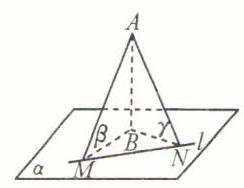
\includegraphics[width=0.2\textwidth]{bodyxb/src/bo_d20aucref24c73anc48g_168_1092_1009_244_188_0.jpg}
    \end{center}
    \begin{jieda}
        \begin{enumerate}
            \item 证明:作 ${BC}\bot {MN}$ 于点 $C$ ,连接 ${AC}$ . 作 ${BH}\bot {AC}$ 于点 $H$ ,连接 ${MH}$ . ${AB}\bot \alpha$. $\therefore {AB}\bot {MN}$ ,又 ${BC}\bot {MN},\therefore {MN}\bot$ 平面 ${ABC},\therefore {MN}\bot {AC},{MN}\bot {BH}$ . 又 ${BH}\bot {AC},\therefore {BH}\bot$ 平面 ${AMN},\therefore {BH} \bot  {AN}.\beta  \bot  \gamma ,\beta  \cap  \gamma  = {AB},{MB} \bot  {AB},\therefore {MB} \bot$ 平面 ${ABN},\therefore {MB} \bot  {AN}$ . 又 ${BH} \cap  {MB}$  $= B,\therefore {AN} \bot$ 平面 ${MBH},\therefore {AN} \bot  {MH}$ ,即定点 $H$ 为 $\bigtriangleup {AMN}$ 的垂心,证毕.
            \item $\bigtriangleup  {ABM}, \bigtriangleup  {ABN}, \bigtriangleup  {MBN}$ 是直角三角形. 由勾股定理, $A{M}^{2} + A{N}^{2} - M{N}^{2} = \left( {A{B}^{2} + B{M}^{2}}\right)  + \left( {A{B}^{2} + B{N}^{2}}\right)  -$  $\left( {B{M}^{2} + B{N}^{2}}\right)  = 2 \cdot  A{B}^{2}$ 为定值,证毕.
        \end{enumerate}
    \end{jieda}
\end{enumerate}
\begin{center}  \textbf{(C)} \end{center}
\begin{enumerate}
    \item 在正方体 ${ABCD} - {A}_{1}{B}_{1}{C}_{1}{D}_{1}$ 中,根据给出的条件,分别画出截面图形:
    \begin{enumerate}
        \item 过 $A,C$ 和 $D{D}_{1}$ 延长线上一点 $P$ (如图)

        \begin{center}
            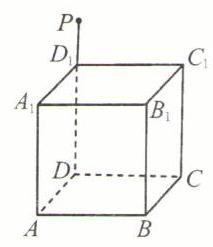
\includegraphics[width=0.2\textwidth]{bodyxb/src/bo_d20aucref24c73anc48g_168_347_1841_213_247_0.jpg}
        \end{center}

        \item 过 ${AB}$ , $C{C}_{1}$ 的中点 $P$ , $Q$ 及 ${D}_{1}$ (如图)

        \begin{center}
        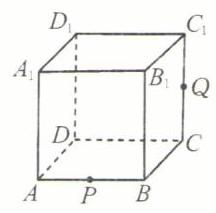
\includegraphics[width=0.2\textwidth]{bodyxb/src/bo_d20aucref24c73anc48g_168_722_1875_216_213_0.jpg}
        \end{center}

        \item 过 ${AB},C{C}_{1}$ 和 ${C}_{1}{D}_{1}$ 的中点 $P,Q,R$ (如图)

        \begin{center}
        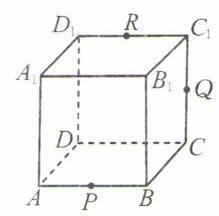
\includegraphics[width=0.2\textwidth]{bodyxb/src/bo_d20aucref24c73anc48g_168_1096_1869_219_216_0.jpg}
        \end{center}
    \end{enumerate}
    \begin{jieda}
        \threetu{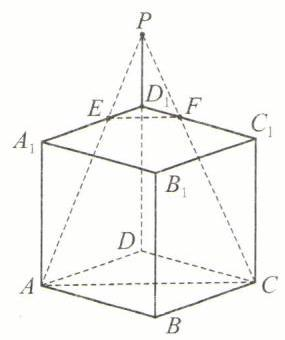
\includegraphics[width=0.6\textwidth]{bodyxb/src/bo_d20cdrf7aajc73bfmvhg_137_216_929_285_340_0.jpg}}{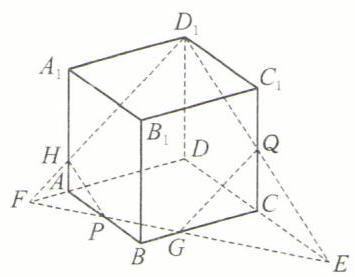
\includegraphics[width=0.7\textwidth]{bodyxb/src/bo_d20cdrf7aajc73bfmvhg_137_534_992_355_277_0.jpg}}{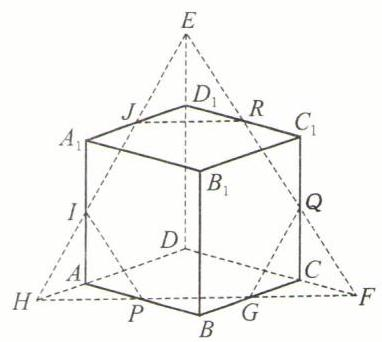
\includegraphics[width=0.7\textwidth]{bodyxb/src/bo_d20cdrf7aajc73bfmvhg_137_922_927_382_342_0.jpg}}
    \end{jieda}
    \item 在正方体 ${ABCD} - {A}_{1}{B}_{1}{C}_{1}{D}_{1}$ 中, $M,N,P,Q,R,S$ 分别是棱 ${AB},{BC},C{C}_{1},{C}_{1}{D}_{1}$ , ${A}_{1}{D}_{1},A{A}_{1}$ 的中点 (如图),试证明: ${MNPQRS}$ 是一个平面图形.

    \begin{center}
    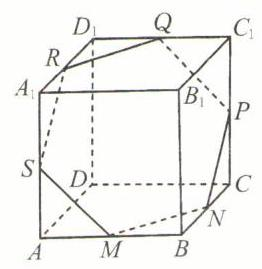
\includegraphics[width=0.2\textwidth]{bodyxb/src/bo_d20aucref24c73anc48g_169_633_269_262_269_0.jpg}
    \end{center}
    \begin{jieda}
        ${MN}$ 是 $\bigtriangleup {ABC}$ 中 ${AC}$ 边对应的中位线, $\therefore {MN}//{AC}, {SA} //{PC}$ ,四边形 ${SACP}$ 是平行四边形, ${MN}//{AC}//{SP}$ ; 同理, ${RQ}//{A}_{1}{C}_{1}//{SP},{RQ}//{SP}//{MN}$ . 类似地,有 ${RS}//{QM}//{PN}$ 和 ${PQ}//{NR}//{MS}$ .
        
        记 $S,R,Q$ 三点确定的平面为 $\alpha$ ,由 ${RQ}//{SP}$ 及公理 2 的推论 3 (经过两条平行直线,有且只有一个平面) 可知 $P$  ${ \in  } {\alpha }$ . 同理, $\because {RS}//{PN},\therefore N{ \in  } {\alpha }.\because {RQ}//{MN},\therefore M{ \in  } {\alpha },\therefore M,N,P,Q,R,S$ 六点共面,证毕.
    \end{jieda}

    \item 已知点 $O$ 不在空间四边形 ${ABCD}$ 四边所在的直线上,且 ${CD}$ 交面 ${OAB}$ 于 $E,{DA}$ 交面 ${OBC}$ 于 $F,{AB}$ 交面 ${OCD}$ 于 $G,{BC}$ 交面 ${OAD}$ 于 $H$ (如图),求证 $E,F,G,H$ 四点共面.

    \begin{center}
    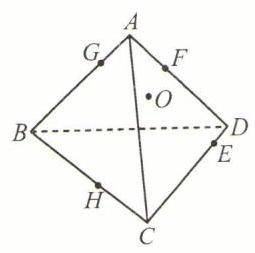
\includegraphics[width=0.2\textwidth]{bodyxb/src/bo_d20aucref24c73anc48g_169_215_761_255_253_0.jpg}
    \end{center}
    \begin{jieda}
        证明:点 $H \in$ 平面 ${OAD}$ ,点 $F \in  {AD} \subset$ 平面 ${OAD}$ ,由公理 $1,{HF} \subset$ 平面 ${OAD}$ ,同理 ${HF} \subset$ 平面 ${OBC}$ . 又点 $O \in$ 平面 ${OAD}$ ,点 $O \in$ 平面 ${OBC}$ ,由公理 3,点 $O \in$ 平面 ${OAD} \cap$ 平面 ${OBC} =$ 直线 ${HF}$ ；同理,点 $O \in$ 直线 ${GE}$ ；由公理 2 的推论 2, $E,F,G,H$ 四点共面,证毕.
    \end{jieda}
    \item \begin{enumerate}
        \item 在四面体 ${DABC}$ 中, $M,N,P,R,Q,S$ 分别是 ${DC},{AB},{DA},{DB},{BC},{CA}$ 的中点, 求证: ${PQ},{RS},{MN}$ 共点 (如图)

        \begin{center}
        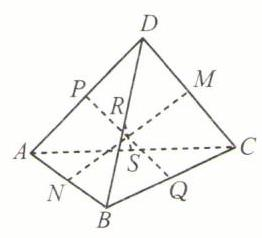
\includegraphics[width=0.2\textwidth]{bodyxb/src/bo_d20aucref24c73anc48g_169_631_774_262_238_0.jpg}
        \end{center}
        \begin{jieda}
            证明: ${PN} \overset{//}{=} \dfrac{1}{2}{DB},{MQ} \overset{//}{=} \dfrac{1}{2}{DB},\therefore {PN} \overset{//}{=} {MQ},\therefore$ 四边形 ${PNQM}$ 是平行四边形,
            
            $\therefore {PQ},{MN}$ 共面,交点为线段 ${MN}\left( {PQ}\right)$ 的中点,记为 $O$ . 类似地,可以证明四边形 ${RNSM}$ 是平行四边形. $\therefore {RS},{MN}$ 共面,且 ${RS}$ 也过线段 ${MN}$ 的中点,即: ${PQ},{RS},{MN}$ 共点 $O$ ,证毕.
        \end{jieda}
        \item 在四面体 ${ABCD}$ 中, ${O}_{1},{O}_{2},{O}_{3},{O}_{4}$ 分别是 $\bigtriangleup {ACD},\bigtriangleup {BCD},\bigtriangleup {ABC},\bigtriangleup {ABD}$ 的重心 (如图),求证: $B{O}_{1},A{O}_{2},D{O}_{3},C{O}_{4}$ 交于一点.

        \begin{center}
        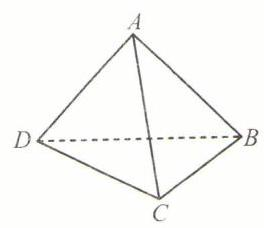
\includegraphics[width=0.2\textwidth]{bodyxb/src/bo_d20aucref24c73anc48g_169_1055_775_264_228_0.jpg}
        \end{center}
        \begin{jieda}
            证明:先确定 $B{O}_{1}$ 和 $A{O}_{2}$ 的交点位置. 取 ${CD}$ 边的中点 $E$ ,连接 ${AE}$ , ${BE}$ ,由题意 ${O}_{1} \in  {AE} \subset$ 平面 ${AEB}$ , ${O}_{2} \in  {BE} \subset$ 平面 ${AEB}$ ,由公理 $1,B{O}_{1}$ 和 $A{O}_{2}$ 都在平面 ${AEB}$ 内. 记 $B{O}_{1} \cap  A{O}_{2} =$ 点 $O$ ,由重心的性质,有 $\dfrac{E{O}_{1}}{{O}_{1}A} = \dfrac{E{O}_{2}}{{O}_{2}B} = \dfrac{1}{2}$ , $\therefore {O}_{1}{O}_{2}//{AB}$ ,且 $\vv{{O}_{2}O} = \dfrac{1}{4} \cdot  \vv{{O}_{2}A}$ . 再由 $A{O}_{2}$ 为媒介,证明四线共点. 取 ${CB}$ 边的中点 $F$ ,连接 ${DF},{AF}$ ,同理可证 $D{O}_{3}$ 和 $A{O}_{2}$ 都在平面 ${ADF}$ 内,记 $D{O}_{3} \cap  A{O}_{2} =$ 点 ${O}^{\prime }$ ,则由 $\vv{{O}_{2}{O}^{\prime }} = \dfrac{1}{4} \cdot  \vv{{O}_{2}A}$ ,可知 ${O}^{\prime }$ 与 $O$ 是同一点,同理 $C{O}_{4}$ 和 $A{O}_{2}$ 也共面,且交点为 $O$ . 综上, $B{O}_{1},A{O}_{2},D{O}_{3},C{O}_{4}$ 交于同一点 $O$ ,证毕.
        \end{jieda}
    \end{enumerate}
    \item 平行四边形${ABCD}$ 的顶点 $A$ 在锐二面角 $\alpha  - {MN} - \beta$ 的棱上, $B,C,D$ 都在 $\alpha$ 内,且 ${AB} = {2AD},\angle {DAN} = {45}^{ \circ  },\angle {BAD} = {60}^{ \circ  }$ (如图),求二面角 $\theta$ 的余弦值,使 $平行四边形{ABCD}$ 在半平面 $\beta$ 上的射影是\begin{enumerate*}
        \item 菱形
        \item 矩形
    \end{enumerate*}
    \begin{center}
    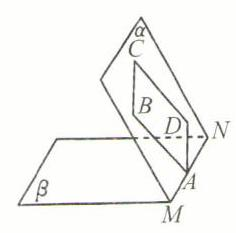
\includegraphics[width=0.2\textwidth]{bodyxb/src/bo_d20aucref24c73anc48g_169_1190_1318_236_233_0.jpg}
    \end{center}
    \begin{jieda}
        $\angle {BAM} = {75}^{ \circ  }$ . 作 $B{B}^{\prime }\bot \beta$ 于点 ${B}^{\prime },C{C}^{\prime }\bot \beta$ 于点 ${C}^{\prime },D{D}^{\prime }\bot \beta$ 于点 ${D}^{\prime }$ . 在线段 $C{C}^{\prime }$ 上取点 $E$ ,使得 ${CE} = B{B}^{\prime }$ . 下证四边形$A{B}^{\prime }{C}^{\prime }{D}^{\prime }$ 是平行四边形. 
        
        ${CE}\overset{//}{=} {BB}^{\prime },\therefore$ 四边形 ${CE}{B}^{\prime }B$ 是平行四边形, $\therefore {BC}\overset{//}{=} B^{\prime }E$ ,又 ${BC}\overset{//}{=} {AD}^{\prime },\therefore$ 四边形 ${ADE}{B}^{\prime }$ 是平行四边形, ${AD} \overset{//}{=}  {B}^{\prime }E,{ED} \overset{//}{=} {B}^{\prime }A$ . 在 Rt $\bigtriangleup  E{C}^{\prime }{B}^{\prime }$ 和 Rt $\bigtriangleup  D{D}^{\prime }A$ 中,由 $E{B}^{\prime }//{DA},E{C}^{\prime }//D{D}^{\prime }$ ,得 $\angle {B}^{\prime }E{C}^{\prime } =$  $\angle {AD}{D}^{\prime }$ ,又 $\because \angle E{C}^{\prime }{B}^{\prime } = \angle D{D}^{\prime }A = {90}^{ \circ  },E{B}^{\prime } = {DA}\therefore \bigtriangleup E{C}^{\prime }{B}^{\prime } \cong  \bigtriangleup D{D}^{\prime }A$ , $\therefore E{C}^{\prime } \overset{//}{=} D{D}^{\prime }$ . $\therefore$ 四边形 ${ED}{D}^{\prime }{C}^{\prime }$ 是平行四边形, ${ED}\overset{//}{ = }{C}^{\prime }{D}^{\prime }$ . 又 ${ED}\overset{//}{ = }{B}^{\prime }A,\therefore$ 四边形 $A{B}^{\prime }{C}^{\prime }{D}^{\prime }$ 是平行四边形,证毕.
        
        在平面 $\alpha$ 中作 ${BH} \bot  {MN}$ 于 $H,{DF} \bot  {MN}$ 于 $F$ ,连接 $H{B}^{\prime },F{D}^{\prime }$ ,则 $H{B}^{\prime } \bot  {MN},F{D}^{\prime } \bot  {MN}$，因此$\angle {BH}{B}^{\prime }$ 和 $\angle {DF}{D}^{\prime }$ 都是二面角 $\alpha  - {MN} - \beta$ 的平面角. 
        
        设 ${AD} = 1$ ,则 ${AB} = 2;{BH} = 2 \cdot  \sin {75}^{ \circ  },{DF} = \dfrac{\sqrt{2}}{2};B{B}^{\prime } = {BH} \cdot  \sin \theta  = 2 \cdot  \sin {75}^{ \circ  } \cdot  \sin \theta ,D{D}^{\prime } = {DF} \cdot$  $\sin \theta  = \dfrac{\sqrt{2}}{2}\sin \theta .$
        \begin{enumerate}
            \item 平行四边形 $A{B}^{\prime }{C}^{\prime }{D}^{\prime }$ 是菱形的充要条件是 $A{B}^{\prime } = A{D}^{\prime }.A{B}^{\prime 2} = A{B}^{2} - B{B}^{\prime 2} = 4 - 4 \cdot  {\sin }^{2}{75}^{ \circ  } \cdot  {\sin }^{2}\theta ,A{D}^{\prime 2} = A{D}^{2} -$  $D{D}^{\prime 2} = 1 - \dfrac{1}{2} \cdot  {\sin }^{2}\theta$ . 由 $A{B}^{\prime 2} = A{D}^{\prime 2}$ ,解得 ${\sin }^{2}\theta  = 4\sqrt{3} - 6,\therefore {\cos }^{2}\theta  = 7 - 4\sqrt{3},\therefore \cos \theta  = 2 - \sqrt{3}$ .
            
            \item 平行四边形 $A{B}^{\prime }{C}^{\prime }{D}^{\prime }$ 是矩形的充要条件是 $A{B}^{\prime } \bot  A{D}^{\prime }$ . 考察四边形 ${D}^{\prime }{FE}{B}^{\prime },E{B}^{\prime } \bot  {MN},F{D}^{\prime } \bot  {MN}$ ,又 ${BE} \neq  {DF}$. $\therefore$ 四边形 ${D}^{\prime }{FE}{B}^{\prime }$ 是直角梯形. $A{B}^{\prime }\bot A{D}^{\prime }$ 时,易证: $\bigtriangleup {D}^{\prime }{FA}\infty \bigtriangleup {AE}{B}^{\prime },\therefore \dfrac{{D}^{\prime }F}{FA} = \dfrac{AE}{E{B}^{\prime }}$ ,得 $\dfrac{{DF} \cdot  \cos \theta }{FA} = \dfrac{AE}{{EB} \cdot  \cos \theta }$ , 即 ${\cos }^{2}\theta  = \dfrac{1}{\tan {45}^{ \circ  } \cdot  \tan {75}^{ \circ  }},\therefore \cos \theta  = \dfrac{\sqrt{6} - \sqrt{2}}{2}$ .
        \end{enumerate}
    \end{jieda}
    \item \begin{enumerate}
        \item 在棱长为 1 的正方体 ${ABCD} - {A}_{1}{B}_{1}{C}_{1}{D}_{1}$ 中,点 $P$ 在面对角线 ${AC}$ 上,记二面角 $P - {A}_{1}{B}_{1} - {C}_{1}$ 为 $\alpha$ ,二面角 $P - {B}_{1}{C}_{1} - {A}_{1}$ 为 $\beta$ (如图). \ding{172}记线段 ${AP},{CP}$ 的长度分别为 $s,t$ ,试用 $s,t$ 表示 $\tan \left( {\alpha  + \beta }\right)$ , \ding{173} 求 $\tan \left( {\alpha  + \beta }\right)$ 最小时点 $P$ 的位置
        \begin{center}
        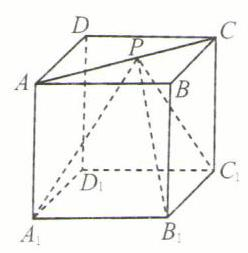
\includegraphics[width=0.2\textwidth]{bodyxb/src/bo_d20aucref24c73anc48g_169_695_1842_248_253_0.jpg}
        \end{center}
        \begin{jieda}
            连接 ${A}_{1}{C}_{1}$ ,在线段 ${A}_{1}{C}_{1}$ 上取 ${A}_{1}Q = {AP}$ ,连接 ${PQ}$ ,并作 ${QE}\bot {A}_{1}{B}_{1}$ 于点 $E$ , ${QF}\bot {B}_{1}{C}_{1}$ 于点 $F$ ,连接 ${PE}$ , ${PF}$ .$\because {AP} \overset{//}{=} {A}_{1}Q,\therefore$ 四边形 ${APQ}{A}_{1}$ 是平行四边形, $\therefore {PQ} \bot$ 平面 ${A}_{1}{B}_{1}{C}_{1}{D}_{1}$ . 由三垂线定理,得 ${PE} \bot  {A}_{1}{B}_{1}$ , ${PF} \bot  {B}_{1}{C}_{1},\therefore \angle {PEQ} = \alpha ,\angle {PFQ} = \beta$ . 
            
            \ding{172} $\tan \alpha  = \dfrac{PQ}{EQ} = \dfrac{1}{\dfrac{\sqrt{2}}{2}s} = \dfrac{\sqrt{2}}{s},\tan \beta  = \dfrac{PQ}{FQ} = \dfrac{1}{\dfrac{\sqrt{2}}{2}t} = \dfrac{\sqrt{2}}{t},\therefore \tan \left( {\alpha  + \beta }\right)  =$  $\dfrac{\tan \alpha  + \tan \beta }{1 - \tan \alpha  \cdot  \tan \beta } = \dfrac{2}{{st} - 2}\left( {s,t \neq  0}\right)$ . 当 $s = 0$ 或 $t = 0$ 时, $\tan \left( {\alpha  + \beta }\right)  = \tan {135}^{ \circ  } =  - 1$ ,也符合. 综上, $\tan \left( {\alpha  + \beta }\right)  = \dfrac{2}{{st} - 2}$ .

            \ding{173} $\because \tan \left( {\alpha  + \beta }\right)  = \dfrac{2}{s\left( {\sqrt{2} - s}\right)  - 2} = \dfrac{2}{-{\left( s - \dfrac{\sqrt{2}}{2}\right) }^{2} - \dfrac{3}{2}},s \in  \left\lbrack  {0,\sqrt{2}}\right\rbrack  ,\therefore \tan \left( {\alpha  + \beta }\right)$ 的值域为 $\left\lbrack  {-\dfrac{4}{3}, - 1}\right\rbrack$. $\therefore$ 当 $s = \dfrac{\sqrt{2}}{2} = t$ ,即 $P$ 取 ${AC}$ 中点时, $\tan \left( {\alpha  + \beta }\right)$ 有最小值 $- \dfrac{4}{3}$ .
        \end{jieda}
        \item 已知 $P$ 是棱长为 $a$ 的正方体 ${A}_{1}{B}_{1}{C}_{1}{D}_{1} - {ABCD}$ 的棱 ${AD}$ 上的动点(如图)
        
        \ding{172}画出过点 $B,P,{D}_{1}$ 的截面,判断截面的形状,并证明你的结论, \ding{173}求截面面积的最小值,并证明你的结论.
        \begin{center}
        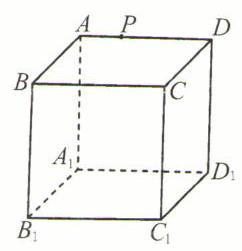
\includegraphics[width=0.2\textwidth]{bodyxb/src/bo_d20aucref24c73anc48g_170_784_204_242_251_0.jpg}
        \end{center}
        \begin{jieda}
            \ding{172} 在线段 ${B}_{1}{C}_{1}$ 上取 ${C}_{1}Q = {PA}$ ,下证:连接 $B,P,{D}_{1},Q$ 所得的图形即为所求截面. 在线段 ${A}_{1}{D}_{1}$ 上取 ${A}_{1}{P}^{\prime } = {AP}$ ,则 $P{P}^{\prime }\overset{//}{ = }A{A}_{1}\overset{//}{ = }B{B}_{1},\therefore$ 四边形 ${BP}{P}^{\prime }{B}_{1}$ 是平行四边形, $\therefore {BP}\overset{//}{ = }{B}_{1}{P}^{\prime }$ . 再由 $\bigtriangleup {B}_{1}{A}_{1}{P}^{\prime } \cong  \bigtriangleup {D}_{1}{C}_{1}Q$ ,可证 ${D}_{1}Q\overset{//}{ = }$  ${B}_{1}{P}^{\prime },\therefore {D}_{1}Q \overset{//}{=} {BP},\therefore$ 四边形 ${BP}{D}_{1}Q$ 是封闭的平面图形,且为平行四边形,证毕.

            \ding{173} $\because S = 2{S}_{\bigtriangleup {BQ}{D}_{1}} = \left( {\dfrac{1}{2} \times  B{D}_{1} \cdot  {QH}}\right)  \times  2 = \sqrt{3}a \cdot  {QH}\left( Q\right.$ 为截面与 ${B}_{1}{C}_{1}$ 的交点, $\left. {{QH}\bot B{D}_{1}\text{ 于点 }H}\right)$ , $\therefore$ 只需求 ${QH}$ 的最小值,即 ${B}_{1}{C}_{1}$ 到面 ${BC}{D}_{1}{A}_{1}$ 的距离,为 $\dfrac{\sqrt{2}}{2}a,\therefore {S}_{\min } = \dfrac{\sqrt{6}}{2}{a}^{2}$ . 此时 $Q$ 为 ${B}_{1}{C}_{1}$ 的中点,而 $P$ 为 ${AD}$ 的中点.
        \end{jieda}
    \end{enumerate}

    \item $A,B$ 分别是 ${60}^{ \circ  }$ 的二面角 $\alpha  - l - \beta$ 的面 $\alpha ,\beta$ 上的点, $A{A}_{1} \bot  \beta$ 于点 ${A}_{1}$ , $B{B}_{1} \bot  \alpha$ 于点 ${B}_{1}$ ,点 ${A}_{1},{B}_{1}$ 到 $l$ 的距离分别为 $a,b$ ,点 $A,B$ 在棱 $l$ 上的射影间的距离为 $c$ (如图),求 ${AB}$ 的长.

    \begin{center}
    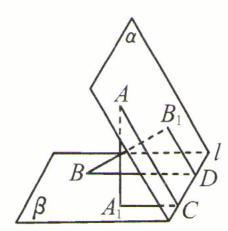
\includegraphics[width=0.2\textwidth]{bodyxb/src/bo_d20aucref24c73anc48g_170_1256_672_228_231_0.jpg}
    \end{center}
    \begin{jieda}
        作 ${A}_{1}C \bot  l$ 于点 $C,{B}_{1}D \bot  l$ 于点 $D$ ,连接 ${AC},{BD},A{A}_{1} \bot  \beta$ ,又 ${A}_{1}C \bot  l$ ,由三垂线定理得 ${AC} \bot  l,\therefore \angle {AC}{A}_{1}$ 是二面角 $\alpha  - l - \beta$ 的平面角. 同理 ${BD} \bot  l,\angle {BD}{B}_{1}$ 也是二面角 $\alpha  - l - \beta$ 的平面角. 在直角梯形 (或矩形) ${A}_{1}{CDB}$ 中, ${A}_{1}{B}^{2} =$  $C{D}^{2} + {\left( BD - {A}_{1}C\right) }^{2} = {c}^{2} + {\left( 2b - a\right) }^{2},\therefore A{B}^{2} = A{A}_{1}^{2} + {A}_{1}{B}^{2} = {\left( \sqrt{3}a\right) }^{2} + {c}^{2} + {\left( 2b - a\right) }^{2},\therefore {AB}$  $= \sqrt{4\left( {{a}^{2} - {ab} + {b}^{2}}\right)  + {c}^{2}}$ .
    \end{jieda}
\end{enumerate}
    



\section*{* 五、异面直线间的距离}

\subsubsection*{【典型题型与解题技巧】}

求异面直线间的距离

定理 对于任意给定的两条异面直线, 存在唯一的一条直线与这两条直线都垂直并且相交. 这条直线称为这两条异面直线的公垂线, 公垂线的两个垂足之间的线段称为异面直线的公垂线段,两条异面直线的公垂线段的长度就叫做两条异面直线间的距离.

\textbf{例 1} 如图，已知正方体 ${ABCD} - {A}_{1}{B}_{1}{C}_{1}{D}_{1}$ 的棱长为 1 .

\begin{center}
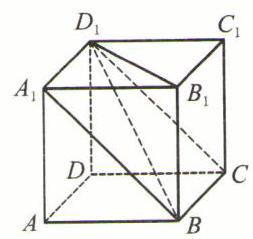
\includegraphics[width=0.2\textwidth]{bodyxb/src/bo_d20aucref24c73anc48g_171_1183_588_253_239_0.jpg}
\end{center}

(1)求异面直线 $A{A}_{1}$ 与 ${D}_{1}{B}_{1}$ 的距离；

(2)求异面直线 ${AD}$ 与 $B{D}_{1}$ 的距离.

\textbf{解}

(1)连接 ${A}_{1}{C}_{1}$ 交 ${B}_{1}{D}_{1}$ 于点 $O$ ,则 ${A}_{1}O \bot  {A}_{1}A$ , ${A}_{1}O \bot  {B}_{1}{D}_{1}$ ,所以 ${A}_{1}{O}_{1}$ 为 ${A}_{1}A$ 与 ${D}_{1}{B}_{1}$ 的公垂线段,异面直线 $A{A}_{1}$ 与 ${D}_{1}{B}_{1}$ 的距离为 ${A}_{1}{O}_{1} = \dfrac{\sqrt{2}}{2}$ .

(2)因为 ${AD}//{BC}$ ,而 ${BC}$ 在平面 ${A}_{1}{BC}{D}_{1}$ 上,所以 ${AD}//$ 平面 ${A}_{1}{BC}{D}_{1}$ . 又因为 $B{D}_{1}$ 在平面 ${A}_{1}{BC}{D}_{1}$ 上,所以异面直线直线 ${AD}$ 与 $B{D}_{1}$ 的距离即等于点 $A$ 到平面 ${A}_{1}{BC}{D}_{1}$ 的距离,其值为 $\dfrac{\sqrt{2}}{2}$ .

\subsubsection*{【训练题】}

\begin{center}  \textbf{(A)} \end{center}
\begin{enumerate}
    \item 已知 ${EF}$ 是异面直线 $a,b$ 的公垂线,直线 $l//{EF}$ ,则 $l$ 与 $a,b$ 交点的个数是 \dotfill{(\kh{C})}
    \xx{0}{1}{0 或 1}{0,1或 2}
    \begin{jieda}
        $l$ 与 $a,b$ 不可能有两个交点,否则异面直线 $a,b$ 将同在由 ${EF}$ 与 $l$ 确定的平面内,矛盾. 以正方体 ${ABCD}$  ${A}^{\prime }{B}^{\prime }{C}^{\prime }{D}^{\prime }$ 为例,取 $a = {AB},b = {A}^{\prime }{D}^{\prime },{EF} = A{A}^{\prime }$ ,若取 $l = C{C}^{\prime }$ 则交点个数为 0 : 若取 $l = D{D}^{\prime }$ 则交点个数为 1 .
    \end{jieda}
    \item 已知正方体 ${ABCD} - {A}_{1}{B}_{1}{C}_{1}{D}_{1}$ 的棱长为 $a$ ,则棱 ${A}_{1}{B}_{1}$ 所在直线与面对角线 $B{C}_{1}$ 所在直线间的距离是\dotfill{(\kh{A})}
    \xx{$\dfrac{\sqrt{2}}{2}a$}{$a$}{$\sqrt{2}a$}{$\dfrac{a}{2}$}
    \begin{jieda}
        连接 ${B}_{1}C$ ,与 $B{C}_{1}$ 交于点 $E$ ,不难得到 ${B}_{1}C \bot  B{C}_{1}$ . 又 ${A}_{1}{B}_{1} \bot$ 平面 ${BC}{C}_{1}{B}_{1}$ ,故 ${A}_{1}{B}_{1} \bot  {B}_{1}C,\therefore {A}_{1}{B}_{1}$ 与 $B{C}_{1}$ 的公垂线段为 ${B}_{1}E,{B}_{1}E = \dfrac{\sqrt{2}}{2}a$ .
    \end{jieda}
    \item 已知直线 $a,b,c$ 中任何两条都是相互垂直的异面直线, $d$ 是 $b,c$ 的公垂线,则\dotfill{(\kh{C})}
    \xx{$d$ 与 $a$ 是互相垂直的异面直线}{$d$ 与 $a$ 是相交直线}{$d$ 与 $a$ 是平行直线}{$d$ 与 $a$ 可能平行也可能相交}
    \begin{jieda}
        $a//d$ 必然成立,证明如下: 在直线 $b$ 上任取一点 $P$ ,在点 $P$ 和直线 $c$ 确定的平面中,过点 $P$ 作直线 $c$ 的平行线 ${c}^{\prime }$ (即平移直线 $c$ ,使之经过点 $P$ ). 由相交直线 $b$ 和 ${c}^{\prime }$ 确定的平面记作 $\alpha$ . 易证: $a\bot \alpha ,d\bot \alpha$ ,又由公垂线的定义, $a,d$ 不可能重合,故 $a//d$ . 证毕. 
        
        \ps 本题的关键是构造出辅助平面 $\alpha$ .
    \end{jieda}
    \item 若平面 $\alpha //$ 平面 $\beta$ ,直线 $l \subset  \alpha$ ,且 $\alpha$ , $\beta$ 间的距离为 $d$ ,有下列四个命题:\ding{172} $\beta$ 内有且只有一条直线与 $l$ 的距离等于 $d$ ；\ding{173} $\beta$ 内所有直线与 $l$ 的距离都等于 $d$ ；\ding{174} $\beta$ 内有无数条直线与 $l$ 的距离等于 $d$ ；\ding{175} $\beta$ 内所有直线与 $\alpha$ 的距离都等于 $d$ . 其中正确的是 \dotfill{(\kh{D})}
    \xx{\ding{172}}{\ding{173}}{\ding{172}和\ding{175}}{\ding{174}和\ding{175}}
    \begin{jieda}
        记 $l$ 在平面 $\beta$ 内的射影是 ${l}^{\prime },m$ 是平面 $\beta$ 内的任意一条直线,直线 $l,m$ 的距离为 $x$ . 当 $m$ 与 ${l}^{\prime }$ 重合时,显然 $x = d$ ; 当 $m/{l}^{\prime }$ 时,显然 $x > d$ ；当 $m$ 与 ${l}^{\prime }$ 相交时,两直线的公垂线(段)同时也是平面 $\alpha ,\beta$ 的公垂线(段),因此 $x = d$ . (具体作法:记 $m \cap  {l}^{\prime } = A$ ,在点 $A$ 和直线 $l$ 确定的平面中,作 ${AB}\bot l$ 于点 $B$ ,线段 ${AB}$ 即为公垂线段). 因此\ding{172}\ding{173}错误,\ding{174}正确,\ding{175}正确,因为 $\alpha //\beta ,\therefore \beta$ 内任意直线 $n$ 都与 $\alpha$ 平行,因此直线 $n$ 到平面 $\alpha$ 的距离转化为 $n$ 上任意一点到 $\alpha$ 的距离,即为 $d$ .
    \end{jieda}
    \item 直线 $a,b$ 异面,与 $a,b$ 都垂直的直线有\blkda{无数}条； $a,b$ 的公垂线有\blkda{1}条.
    
    \item 如图,正方体 ${ABCD} - {A}_{1}{B}_{1}{C}_{1}{D}_{1}$ 的棱长是 1,则
    
    \begin{center}
    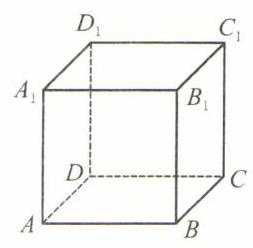
\includegraphics[width=0.2\textwidth]{bodyxb/src/bo_d20aucref24c73anc48g_172_1242_182_253_248_0.jpg}
    \end{center}
    \begin{enumerate}
        \item 异面直线 ${A}_{1}B$ 与 ${CD}$ 之间的距离为\blkda{1}
        \item 异面直线 ${A}_{1}B$ 与 ${C}_{1}D$ 之间的距离为\blkda{1}
        \item 异面直线 ${A}_{1}B$ 与 ${B}_{1}{C}_{1}$ 之间的距离为\blkda{$\dfrac{\sqrt{2}}{2}$}
        \item 与 ${AB}$ 异面,且距离为 1 的棱有\blkda{4}条
        \item 与 ${AB}$ 异面,且距离为 1 的面对角线有\blkda{4}条.
    \end{enumerate}
    \item 若正四面体 ${ABCD}$ 的棱长为 1,则对棱所在直线之间的距离为\blkda{$\dfrac{\sqrt{2}}{2}$}
    \begin{jieda}
        分别取 ${BC},{AD}$ 中点 $E,F$ ,连接 ${EF}$ . 易知 ${EF}$ 为 ${BC}$ 与 ${AD}$ 公垂线段,可得 ${EF} = \dfrac{\sqrt{2}}{2}$. 
    \end{jieda}
    \item 已知 $a,b$ 是成 ${60}^{ \circ  }$ 角的一对异面直线,其公垂线段 ${AB} = {10}{{cm}},A \in  a$ . 又 $M \in  a$ ,且 ${AM} =$  $5{{cm}}$ ,则点 $M$ 到 $b$ 的距离等于\blkda{$\dfrac{5\sqrt{19}}{2}$} ${{cm}}$ .
    \begin{jieda}
        过点 $B$ 作直线 $c//a$ ,在 $c$ 上取一点 $C$ ,使得 $\vv{BC} = \vv{AM}$ ,连接 ${AB},{CM}$ ,则四边形 ${AB}$ - ${CM}$ 是平行四边形. 在直线 $b\left( {b}_{1}\right.$ 或 ${b}_{2}$ ,但求解是一致的), $c$ 确定的平面 $\alpha$ 内,作 ${CN} \bot  b$ 于 $N$ ,连接 ${MN}.{MC} \bot$ 平面 $\alpha$ ,故 ${MN}$ 在平面 $\alpha$ 上的射影是 ${CN}$ ,由三垂线定理, ${MN} \bot  b$ ,故 ${MN}$ 即为所求. 不难得到 ${NC} = \dfrac{5\sqrt{3}}{2}{{cm}}$ ,又 ${MC} = {10}{{cm}}$ ,故 ${MN} = \sqrt{N{C}^{2} + M{C}^{2}} = \dfrac{5}{2}\sqrt{19}{{cm}}$ .
        
        \begin{center}
        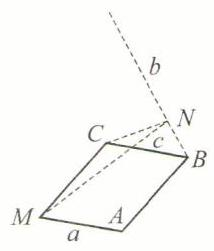
\includegraphics[width=0.2\textwidth]{bodyxb/src/bo_d20cdrf7aajc73bfmvhg_139_1222_1014_214_251_0.jpg}
        \end{center}
    \end{jieda}
    \item 空间四边形 ${ABCD}$ 中, ${AB} = {BD} = {AD} = 2,{BC} = {CD} = 3$ ,延长 ${BC}$ 到 $E$ ,使得 ${BC} = {CE}$ , $F$ 为 ${BD}$ 中点,则异面直线 ${AF}$ 和 ${DE}$ 的距离为\blkda{1}.
    \begin{jieda}
        ${DF}$ 为 ${AF}$ 与 ${DE}$ 的公垂线段且 ${DF} = 1$
    \end{jieda}
    
    \item 菱形 ${ABCD}$ 的边长为 $1,\angle B = \dfrac{\pi }{3}$ ,将此菱形沿对角线 ${AC}$ 折成二面角 $B - {AC} - D$ ,其大小 $\theta  \in  \left\lbrack  {\dfrac{\pi }{3},\dfrac{2\pi }{3}}\right\rbrack$ ,则折后两条对角线 ${AC}$ 与 ${BD}$ 之间的距离 $d$ 的取值范围是\blkda{$\left\lbrack  {\dfrac{\sqrt{3}}{4},\dfrac{3}{4}}\right\rbrack$}.
    \begin{jieda}
        记 ${AC}$ 的中点为 $O$ ,过点 $O$ 作 ${OG} \bot  {BD}$ 于点 $G$ ,易知 ${OG}$ 为 ${AC}$ 与 ${BD}$ 的公垂线段, $\therefore d = {OG} = \dfrac{\sqrt{3}}{2}\cos \dfrac{\theta }{2} \in  \left\lbrack  {\dfrac{\sqrt{3}}{4},\dfrac{3}{4}}\right\rbrack$ .
    \end{jieda}
    
    \item 在棱长为 2 的正方体 ${ABCD} - {A}_{1}{B}_{1}{C}_{1}{D}_{1}$ 中, $E,F$ 分别是 ${A}_{1}{D}_{1}$ 和 $C{C}_{1}$ 的中点. 则异面直线 ${EF}$ 与 ${AB}$ 之间的距离为\blkda{$\dfrac{3\sqrt{2}}{2}$}.
    \begin{jieda}
        取 ${B}_{1}{C}_{1}$ 的中点 $G$ ,连接 ${EG}$ , ${FG}$ ,连接 $B{C}_{1}$ 交 ${FG}$ 于点 $M$ ,易知 ${BM}$ 为公垂线段,且 ${BM} = \dfrac{3\sqrt{2}}{2}$ .
    \end{jieda}
    
    \item 四面体 ${SABC}$ 中, ${SA} = {BC} = {13},{SB} = {AC} = {14},{SC} = {AB} = {15}$ ,则异面直线 ${AS}$ 与 ${BC}$ 的距离为\blkda{$3\sqrt{14}$}.
    \begin{jieda}
        考虑长方体 ${SDCE} - {GBHA}$ ,令 ${SD} = a,{SE} = b,{SG} = c$ ,则 $\left\{  \begin{array}{l} {a}^{2} + {b}^{2} = {225}, \\  {b}^{2} + {c}^{2} = {169},\text{ 得 }a = 3\sqrt{14}\text{ ,即为所求. } \\  {a}^{2} + {c}^{2} = {196}, \end{array}\right.$ 

        \ps 取$AS$中点$P$，$BC$中点$Q$，则$PQ$即为所求，解三角形亦可求得.
    \end{jieda}
    
    \item 在棱长为 1 的正方体 ${ABCD} - {A}_{1}{B}_{1}{C}_{1}{D}_{1}$ 中, $E$ 为 ${D}_{1}{B}_{1}$ 的中点, $M$ 为 ${AC}$ 上一点, $N$ 为 ${DE}$ 上一点, ${MN}$ 的最小值为\blkda{$\dfrac{\sqrt{3}}{3}$}.
    \begin{jieda}
        令 ${AC}$ 交 ${BD}$ 于点 $O$ ,过点 $O$ 作 ${OF}\bot {DE}$ 于点 $F$ ,则 ${OF} = \dfrac{\sqrt{3}}{3}$ 为 ${AC}$ 与 ${DE}$ 的公垂线段.
    \end{jieda}

    \clearpage
    \item 如图,正方体 ${ABCD} - {A}_{1}{B}_{1}{C}_{1}{D}_{1}$ 的棱长是 1,点 $P$ 在线段 $A{D}_{1}$ 上运动,给出以下命题: 
    
    \ding{172} 异面直线 ${A}_{1}P$ 与 $B{C}_{1}$ 间的距离为定值;
    
    \ding{173} 异面直线 ${C}_{1}P$ 与 $C{B}_{1}$ 所成的角为定值；
    
    \ding{174}二面角 $P - B{C}_{1} - D$ 的大小为定值;
    
    \ding{175}点 $P$ 到平面 $B{C}_{1}D$ 的距离为定值.
    
    其中,所有正确命题的序号为\blkda{\ding{172}\ding{173}\ding{174}\ding{175}}.
    
    \begin{center}
    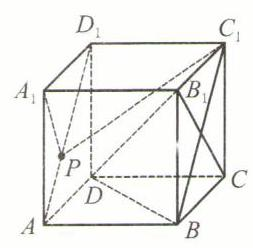
\includegraphics[width=0.2\textwidth]{bodyxb/src/bo_d20aucref24c73anc48g_172_1238_1395_253_248_0.jpg}
    \end{center}
    
    \item 已知 ${EF}$ 是异面直线 $a,b$ 的公垂线段,平面 $\alpha$ 过 ${EF}$ 的中点 $O$ ,且 $a//$  $\alpha ,b//\alpha$ (如图),若 $P,Q$ 分别是 $a,b$ 上任意一点,求证: 线段 ${PQ}$ 被平面 $\alpha$ 平分.
    
    \begin{center}
    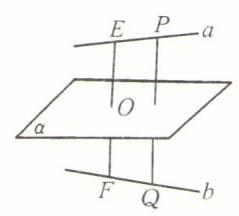
\includegraphics[width=0.2\textwidth]{bodyxb/src/bo_d20aucref24c73anc48g_172_692_1809_239_216_0.jpg}
    \end{center}
    \begin{jieda}
        记线段 ${PQ}$ 与 $\alpha$ 交于点 $R,{PF}$ 与 $\alpha$ 交于点 $S$ ,则 $\dfrac{PR}{RQ} = \dfrac{PS}{SF} = \dfrac{EO}{OF} = 1,\therefore {PR} = {RQ}$ ,证毕.
    \end{jieda}
    
    \item 如图,正四面体 ${ABCD}$ 的棱长为 $a,M,N$ 分别为棱 ${AB},{CD}$ 的中点.
    \begin{enumerate}
        \item 求证: ${MN}$ 是 ${AB},{CD}$ 的公垂线段
        \item 求 ${MN}$ 的长
    \end{enumerate}
    
    \begin{center}
    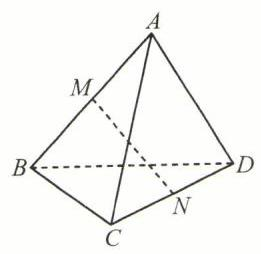
\includegraphics[width=0.2\textwidth]{bodyxb/src/bo_d20aucref24c73anc48g_173_248_318_261_254_0.jpg}
    \end{center}
    \begin{jieda}
        \begin{enumerate}
            \item 证明: 连接 ${MC},{MD},{NA},{NB}$ . 正四面体的四个面是四个全等的正三角形, ${MC},{MD}$ 是中线,故 ${MC} = {MD}$ . 在等腰三角形 ${MCD}$ 中, ${MC} = {MD},{MN}$ 是 ${CD}$ 边上的中线,故 ${MN} \bot  {CD}$ . 同理, ${MN} \bot  {AB}$ . 根据定义, ${MN}$ 是异面直线 ${AB},{CD}$ 的公垂线段. 证毕.
            \item 在 $\bigtriangleup  {MCD}$ 中(也可分析 $\bigtriangleup  {NAB}$ ,过程类似), ${MC} = \dfrac{\sqrt{3}}{2}a$ , ${NC} = \dfrac{1}{2}a$ , ${MN}\bot {CD}$ , $\therefore {MN} = \sqrt{M{C}^{2} - C{N}^{2}} = \dfrac{\sqrt{2}}{2}a$ .
        \end{enumerate}
    \end{jieda}

    \item 如图,已知 ${AB} \bot$ 平面 $\alpha ,B$ 为垂足, ${BC} \subset  \alpha ,{CD} \bot  {BC},{CD}$ 与平面 $\alpha$ 所成角为 ${30}^{ \circ  },{AB} =$  ${BC} = {CD} = 2$ ,且 $A,B,C,D$ 在平面 $\alpha$ 同侧. 求.
    \begin{enumerate}
        \item 异面直线 ${AB}$ 与 ${CD}$ 间的距离
        \item 线段 ${AD}$ 的长
    \end{enumerate}
    \begin{center}
    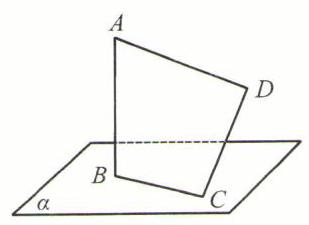
\includegraphics[width=0.2\textwidth]{bodyxb/src/bo_d20aucref24c73anc48g_173_614_346_309_225_0.jpg}
    \end{center}
    \begin{jieda}
        \begin{enumerate}
            \item  ${BC} = 2$ 即为所求.
            \item 作 ${DH} \bot  \alpha$ 于点 $H,\angle {DCH} = {30}^{ \circ  },{DH} = 1,{CH} = \sqrt{3},{BC} \bot  {DC},{BC} \bot  {CH}$ (三垂线), ${BH} = \sqrt{7}$ , ${AD} =$  $\sqrt{{\left( AB - DH\right) }^{2} + B{H}^{2}} = 2\sqrt{2}.$
        \end{enumerate}
    \end{jieda}

    \item $M,N$ 分别是正方体 ${ABCD} - {A}_{1}{B}_{1}{C}_{1}{D}_{1}$ 面对角线 ${A}_{1}B,{B}_{1}{D}_{1}$ 上的点,且 ${A}_{1}M =$  $\dfrac{1}{3}{A}_{1}B,{B}_{1}N = \dfrac{1}{3}{B}_{1}{D}_{1}$ (如图),求证: ${MN}$ 是异面直线 ${A}_{1}B$ 与 ${B}_{1}{D}_{1}$ 的公垂线段.
    
    \begin{center}
    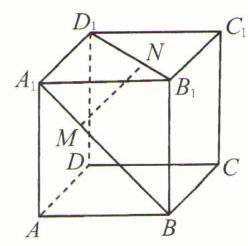
\includegraphics[width=0.2\textwidth]{bodyxb/src/bo_d20aucref24c73anc48g_173_1024_321_248_246_0.jpg}
    \end{center}
    \begin{jieda}
        作 ${MP}\bot {A}_{1}{B}_{1}$ 于点 $P$ ,连接 ${PN}.\because \dfrac{{B}_{1}N}{{B}_{1}{A}_{1}} = \dfrac{\dfrac{\sqrt{2}}{3}}{a} = \dfrac{\sqrt{2}}{3} = \dfrac{{B}_{1}P}{{B}_{1}{D}_{1}} = \dfrac{\dfrac{2}{3}a}{\sqrt{2}a}$ ( $a$ 为正方体边长),又 $\angle N{B}_{1}P =$  $\angle {A}_{1}{B}_{1}{D}_{1},\therefore \bigtriangleup N{B}_{1}P \sim  \bigtriangleup {A}_{1}{B}_{1}{D}_{1},\therefore \angle {PN}{B}_{1} = \angle {D}_{1}{A}_{1}{B}_{1} = {90}^{ \circ  }$ ,即 ${PN} \bot  {B}_{1}{D}_{1}$ ,于是由三垂线定理得 ${MN} \bot  {B}_{1}{D}_{1}$ ,同理可证 ${MN} \bot  {A}_{1}B$ .
    \end{jieda}
    
    \item 已知 ${ABCD}$ 为矩形, $E$ 为半圆 ${CED}$ 上一点,且平面 ${ABCD} \bot$ 平面 ${CDE}$ (如图).
    \begin{enumerate}
        \item 求证: ${DE}$ 是 ${AD}$ 与 ${BE}$ 的公垂线
        \item 若 ${AD} = {DE} = \dfrac{1}{2}{AB}$ ,求 ${AD}$ 和 ${BE}$ 所成角的大小
    \end{enumerate}
        
    \begin{center}
    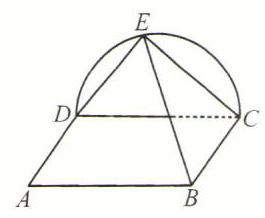
\includegraphics[width=0.2\textwidth]{bodyxb/src/bo_d20aucref24c73anc48g_173_444_1286_265_218_0.jpg}
    \end{center}
    \begin{jieda}
        \begin{enumerate}
            \item $\because {BC} \bot$ 面 ${DEC},{CE}$ 是 ${BE}$ 在面 ${DEC}$ 上的射影,而 ${CE} \bot  {DE}$ , $\therefore {BE} \bot  {DE}$ . 又 $\because {AD} \bot$ 面 ${DEC}$ , $\therefore {AD}$  $\bot  {DE}$ ,故 ${DE}$ 是 ${AD}$ 与 ${BE}$ 的公垂线.
            \item $\because {AD}//{BC}$ , $\therefore$ 锐角 $\angle {EBC}$ 即为所求. 在 Rt $\bigtriangleup {ECB}$ 中, $\angle {ECB} = {90}^{ \circ  },\tan \angle {EBC} = \dfrac{EC}{BC} = \tan \angle {EDC}$ ,易知 $\angle {EBC} = \angle {EDC} = {60}^{ \circ  }$
        \end{enumerate}
    \end{jieda}
    
    \item 已知正方体 ${ABCD} - {A}_{1}{B}_{1}{C}_{1}{D}_{1}$ 的棱长为 $a$ ,求棱 ${B}_{1}{C}_{1}$ 和正方体对角线 $B{D}_{1}$ 间的距离.
        
    \begin{center}
    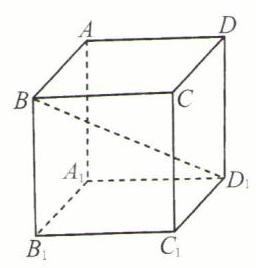
\includegraphics[width=0.2\textwidth]{bodyxb/src/bo_d20aucref24c73anc48g_173_837_1229_256_268_0.jpg}
    \end{center}
    \begin{jieda}
        ${B}_{1}{C}_{1}//$ 平面 ${BC}{D}_{1}{A}_{1}$ ,又 $B{D}_{1} \subset$ 平面 ${BC}{D}_{1}{A}_{1}$ ,设过 ${B}_{1}{C}_{1}$ 且与平面 ${BC}{D}_{1}{A}_{1}$ 平行的平面为 $\alpha$ ,异面直线 ${B}_{1}{C}_{1}$ 和 $B{D}_{1}$ 之间的距离 $= \alpha$ 与平面 ${BC}{D}_{1}{A}_{1}$ 之间的距离 $=$ 点 ${C}_{1}\left( {\alpha \text{ 上任取一点) 与平面 }{BC}{D}_{1}{A}_{1}}\right.$ 之间的距离. 记 ${C}_{1}D \cap$  $C{D}_{1} = O$ ,则 ${C}_{1}O \bot$ 平面 ${BC}{D}_{1}{A}_{1},{C}_{1}O = \dfrac{\sqrt{2}}{2}a$ 即为所求.
    \end{jieda}
    
    \item 在直角梯形 ${ABCD}$ (如图甲)中, ${BC}//{AD},{AD} \bot  {CD},{BC} = 2,{AD} = 3,{CD} = \sqrt{3},{AD}$ 上有一点 $E$ 满足 ${DE} = 1$ . 现将 $\bigtriangleup {ABE}$ 沿 ${BE}$ 所在直线折起到 $\bigtriangleup {A}_{1}{BE}$ 的位置,使平面 ${A}_{1}{BE} \bot $ 平面 ${BCDE}$ ,如图乙所示.
    
    \begin{center}
    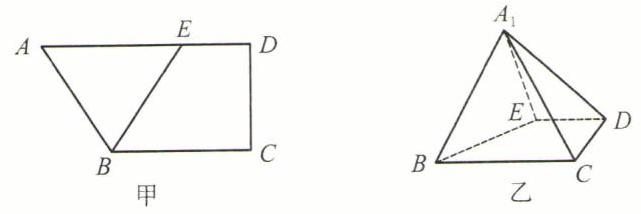
\includegraphics[width=0.5\textwidth]{bodyxb/src/bo_d20aucref24c73anc48g_173_455_1855_641_214_0.jpg}
    \end{center}
    
    \begin{enumerate}
        \item 求证: ${A}_{1}C \bot  {BE}$
        \item 求异面直线 ${A}_{1}C$ 与 ${BE}$ 的距离.
    \end{enumerate} 
    \begin{jieda}
        \begin{enumerate}
            \item ${AE} = {AB} = {BC} = {EC} = 2$ ,菱形 ${AECB}$ 的中心为 $H$ ,折叠前的对角线 ${AHC}\bot {BE}$ ,折叠后, ${A}_{1}H\bot {BE},{CH}\bot {BE}$ ,所以 ${BE} \bot$ 平面 ${A}_{1}{CH},{A}_{1}C \bot  {BE}$ .
            \item ${A}_{1}H = {CH}$ ,作 ${A}_{1}C$ 中点 $M$ ,易知 ${HM}\bot {BE}$ , ${HM}\bot {A}_{1}C$ , ${HM}$ 即为所求. ${A}_{1}H = {CH} = \sqrt{3}$ , ${A}_{1}H\bot {CH}$ (面面垂直性质), ${HM} = \dfrac{\sqrt{6}}{2}$ .
        \end{enumerate}
    \end{jieda}
    
    \item 已知 ${AB}$ 是异面直线 $a,b$ 的公垂线段, $a \subset$ 平面 $\alpha ,b \subset$ 平面 $\beta$ ,且 $\alpha //\beta$ (如图). 求证: ${AB}$ 即平面 $\alpha$ 与平面 $\beta$ 间的距离 (利用此题的结论,可将求两异面直线的距离转化为求两平行平面的距离).
    
    \begin{center}
    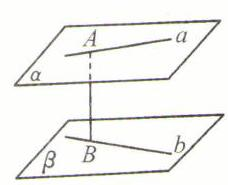
\includegraphics[width=0.2\textwidth]{bodyxb/src/bo_d20aucref24c73anc48g_174_1229_134_228_185_0.jpg}
    \end{center}
    \begin{jieda}
        证明: 记直线 $a$ 和公垂线 ${AB}$ 确定的平面为 $\gamma ,\beta  \cap  \gamma  = {a}^{\prime }.\because \alpha //\beta ,\therefore a//{a}^{\prime }$ 
        
        $\therefore {AB}$ 垂直于平面 $\beta$ 内的两条相交直线 ${a}^{\prime },b,\therefore {AB} \bot$ 平面 $\beta$ . 又 $\alpha //\beta$ ,
        
        $\therefore {AB} \bot$ 平面 $\alpha$ ,可见公垂线段 ${AB}$ 也是平面 $\alpha$ 与平面 $\beta$ 间的距离,证毕.
    \end{jieda}

\end{enumerate}

\begin{center}  \textbf{(B)} \end{center}
\begin{enumerate}
    \item 已知异面直线 $a,b$ 互相垂直,它们的公垂线段 ${PQ} = h$ ,一条长为定值 $m\left( {m > h}\right)$ 的线段 ${AB}$ 两端分别在 $a,b$ 上滑动,求 ${AB}$ 中点 $M$ 的轨迹.
    \begin{jieda}
        如图,不妨将异面直线及其公垂线放在一个正方体 ${QRSP} - {Q}_{1}{R}_{1}{S}_{1}{P}_{1}$ 中,其中 $a$ 即 $Q{Q}_{1},b$ 即 ${PS}$ .
        
        \begin{center}
        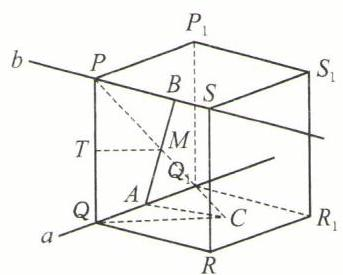
\includegraphics[width=0.2\textwidth]{bodyxb/src/bo_d20cdrf7aajc73bfmvhg_140_1186_1577_343_275_0.jpg}
        \end{center}
        
        \ding{172}当点 $A$ 异于点 $Q$ 且点 $B$ 异于点 $P$ 时,过点 $A$ 作 ${AC}\bot a$ 于点 $A$ ,并使得 $\vv{AC}$  $= \vv{PB}$ ,连接 ${CP},{CQ}$ ,则四边形 ${PBCA}$ 是矩形,其对角线 ${PC},{AB}$ 共面,且交点就是 ${AB}$ 的中点 $M,{PC} = {AB}$ . 取 ${PQ}$ 的中点 $T$ ,连接 ${MT}$ . 在 $\bigtriangleup {PQC}$ 中, ${MT}$ 是 ${CQ}$ 对应的中位线, $\therefore {MT}//{CQ},{MT}//$ 面 ${QR}{R}_{1}{Q}_{1}$ ,即点 $M$ 始终在 ${PQ}$ 的垂直平分面上. 又 $A{B}^{2} =$  $P{C}^{2} = P{Q}^{2} + Q{C}^{2} = {h}^{2} + Q{C}^{2},\therefore {QC} = \sqrt{{m}^{2} - {h}^{2}},\therefore {MT} = \dfrac{1}{2} \cdot  \sqrt{{m}^{2} - {h}^{2}}.$ 
        
        \ding{173} 当点 $A$ 即点 $Q$ 或点 $B$ 即点 $P$ 时,不难证明此时 ${MT}//$ 面 ${QR}{R}_{1}{Q}_{1}$ 和 ${MT} = \dfrac{1}{2} \cdot  \sqrt{{m}^{2} - {h}^{2}}$ 仍然成立. 
        
        \ding{174}下面说明轨迹上的每一点都能取到. 在平面 ${QR}{R}_{1}{Q}_{1}$ 中,以 $Q$ 为圆心, ${QC} = \sqrt{{m}^{2} - {h}^{2}}$ 为半径的圆周上的每一点 $C$ ,作 ${CA} \bot  a$ 于点 $A$ ,并取 $\vv{PB} = \vv{AC}$ ,则 ${AB} = {PC} = \sqrt{P{Q}^{2} + Q{C}^{2}} = \sqrt{{h}^{2} + \left( {{m}^{2} - {h}^{2}}\right) } = m$ . $\bigtriangleup {PQC}$ 中, ${MT}$ 仍是 ${CQ}$ 对应的中位线,即每一点 $C$ 对应一个 $\vv{TM} = \dfrac{1}{2} \cdot  \vv{QC}$ . 综上,点 $M$ 的轨迹是以 ${PQ}$ 的中点 $T$ 为圆心、半径为 $\dfrac{1}{2} \cdot  \sqrt{{m}^{2} - {h}^{2}}$ ,并位于 ${PQ}$ 的垂直平分面上的圆.
    \end{jieda}
    \item 已知 $a,b$ 是异面直线,过 $b$ 作一平面 $\alpha$ ,使 $a//\alpha$ .
    \begin{enumerate}
        \item 写出具体作法
        \item 用反证法证明: $a,b$ 的公垂线只有一条. 并由此证明,四个角都是直角的四边形是矩形.
    \end{enumerate}
    \begin{jieda}
        \begin{enumerate}
            \item 在直线 $b$ 上任取一点 $P$ ,在点 $P$ 和直线 $a$ 确定的平面内,过点 $P$ 作直线 $a$ 的平行线 ${a}^{\prime }$ (可由尺规作图,构造平行四边形得到). 此时,相交直线 ${a}^{\prime }$ 和 $b$ 确定的平面即为平面 $\alpha$ .
            \item 证明:假设 $m,n$ 均为异面直线 $a,b$ 的公垂线,由第 (1) 题的结论,过 $b$ 作一辅助平面 $\alpha$ ,使得 $a//\alpha$ . 由线面垂直的判定定理,有 $m\bot \alpha ,n\bot \alpha$ ; 再由线面垂直的性质定理,有 $m//n$ ,故直线 $m,n$ 可以确定一个平面,结合公垂线的定义及公理 1,可知直线 $a,b$ 也在该平面内,矛盾,故异面直线 $a,b$ 的公垂线唯一. 证毕.

            由此,四个角都是直角的四边形, 任取一组对边, 则另一组对边可以视作它们的公垂线段. 如前所述, 该四边形只能是四个顶点共面的平面图形, 再结合矩形的判定定理, 可知四个角都是直角的四边形一定是矩形. 证毕.
        \end{enumerate}
    \end{jieda}
\end{enumerate}